\documentclass[a4paper,11pt]{article}
\usepackage{jheppub}
\usepackage{graphicx}
\usepackage{amsmath}
\usepackage{amsfonts}
\usepackage{xspace}
\usepackage{hyperref}
\usepackage{placeins}
\usepackage{tikz}
\usepackage{tabularx}
\usepackage{defs}
\usetikzlibrary{arrows.meta,positioning}
\setcounter{topnumber}{1}
\setcounter{bottomnumber}{1}
\setcounter{totalnumber}{2}
\renewcommand{\topfraction}{0.92}
\renewcommand{\bottomfraction}{0.45}
\renewcommand{\textfraction}{0.08}
\renewcommand{\floatpagefraction}{0.85}

\title{Analysis note: precision QCD as a testing ground for precision AI, an agentic measurement of thrust on ALEPH archived data}

\author[a]{ALEPH Reanalysis Team}
\affiliation[a]{Institution list to be finalized}
\emailAdd{to-be-finalized@cern.ch}

\abstract{
High-precision experimental measurements provide an essential testing ground for precision artificial intelligence. As large language models and AI-assisted workflows are increasingly applied to physics calculations and autonomous research, the experimental precision frontier---percent-level measurements with rigorous uncertainty control and full covariance quantification---offers both a validation benchmark and an accountability framework where AI predictions must be quantitative, reproducible, and physically interpretable. Archived LEP1 $e^{+}e^{-}$ data exemplify this regime: the clean initial state, multiple hadronization models, and well-understood detector structure create an ideal sandbox for developing and testing AI-assisted measurement without sacrificing scientific rigor.

This note presents a thrust reanalysis using archived ALEPH data with detector corrections based on Iterative Bayesian Unfolding (RooUnfold), validated through closure tests, refolding checks, iteration-regularization scans, and systematic stability studies. In addition to the unfolded spectrum, complete covariance and correlation matrices are produced for downstream phenomenology use. The workflow itself is framed as an experimental proof-of-concept: we demonstrate that an agentic AI system can execute a full data-driven analysis loop (simulation, reconstruction, unfolding, systematic propagation, documentation) under explicit physicist control and validation checkpoints, with 100\% workflow success and zero required corrections to result-level outputs. The resulting covariance-aware baseline is designed to enable new precision theory--experiment loops in which AI-assisted QCD calculations, tune variants, or novel observables can be directly confronted with high-precision data and held accountable to quantitative constraints. We argue that precision measurements should be understood not only as physics results but as infrastructure for validating the reliability of AI in science.
}

\keywords{QCD, event shapes, electron-positron collisions, unfolding}

\begin{document}
\maketitle
\tableofcontents

\section{Introduction}
\label{sec:introduction}

Machine learning has been central to high-energy physics for decades, enabling
reconstruction algorithms, event classification, and detector optimization across
collider experiments. A new frontier has emerged with large language models (LLMs)
developed by major AI laboratories---including
Anthropic~\cite{Anthropic:2025accelerating}, OpenAI~\cite{OpenAI:2025gpt5science},
Google DeepMind~\cite{GoogleDeepMind:2025geminiscience}, and others---that can now
assist directly with scientific reasoning, mathematical proof, and code generation.
A striking asymmetry persists in fundamental physics: nearly all current
AI-assisted scientific workflows operate on the theoretical or computational side.
Recent examples include AI-assisted derivations of new results in
theoretical particle physics~\cite{OpenAI:2025newresult}, design of novel protein
structures for biology and health research~\cite{GoogleDeepMind:2025alphaproteo},
and assistance with complex mathematical simplifications in high-energy physics
calculations. The experimental side of the AI-assisted scientific loop remains
largely absent. To realize a future where AI rapidly accelerates the discovery of
new physics, AI-assisted scientific workflows must be developed and validated
across \textit{both} precision theory \textit{and} precision experiment.

A logical first step toward closing this gap is an agentic analysis of real
experimental data with expert physicist oversight. This is precisely the approach
pursued here: the physicist opened Anthropic Claude Code, brainstormed the
analysis goals, then iteratively prompted the AI agent to execute the full
analysis workflow. No analysis code was written by hand; the physicist's role is
analogous to advising a graduate student, providing expert direction, reviewing
results, and iterating. The agent was supplied with prior ALEPH analysis code,
analysis notes, and the published paper as context. The rationale follows from
the established understanding in the AI literature that few-shot examples and
supplied context improve AI-assisted outputs~\cite{Brown:2020fewshot,Wei:2022cot}.
Pursuing this theory--experimental interface for physics will inevitably deepen
understanding of AI capabilities and their potential to improve AI systems for
science domains where precision matters.

This vision parallels the evolution of AI in neighboring scientific domains. In
materials science and structural biology, AI work has progressed from computational
prediction with post-hoc human validation toward AI-designed experiments executed
by autonomous robotic systems, creating closed feedback loops where AI proposes,
executes, measures, and learns. High-energy physics faces a parallel opportunity.
While we cannot deploy robotic particle detectors (yet), the emergence of open,
curated data, partially enabled by the e+e$^-$ alliance~\cite{EEAlliance:website},
from past experiments---particularly the precision LEP dataset---can serve as a
``pseudo-laboratory'' for developing and validating AI-assisted scientific workflows
that operate across the precision theory--experiment
interface~\cite{Badea:2019vey,Chen:2021uws}. This requires experimental infrastructure
on both sides: precision theoretical predictions and precision experimental measurements
with rigorous covariance quantification, where AI-assisted reasoning is tested and held
accountable to measurable constraints~\cite{Wang:2023aai,Messeri:2024aiu,Woodruff:2026practicalsi}.

Precision QCD provides an excellent domain for this program, precisely because of the
combination of high-precision $e^{+}e^{-}$ data and sophisticated high-precision theory
calculations. Achieving Standard Model predictions at the precision required for future
collider programs, including the High-Luminosity LHC, demands QCD calculations with
uncertainty control matched to percent-level experimental precision. In this regime,
precision experimental measurement becomes validation infrastructure for AI models.
When percent-level uncertainties are coupled to rigorous covariance quantification and
end-to-end reproducibility, high-precision measurements define the testing ground where
AI predictions are made quantitative, falsifiable, and subject to rigorous scientific
accountability. Although there is currently no active high-energy lepton collider,
archived LEP data now provide an unprecedented open-data opportunity for precision
event-shape studies with explicit uncertainty control~\cite{EEAlliance:website,Badea:2019vey,Chen:2021uws}.
Relative to hadron- and nuclear-collision open-data settings, the LEP $e^{+}e^{-}$
environment provides substantially tighter control of soft-event complexity and
initial-state structure, making it a uniquely clean benchmark for both precision QCD
and precision AI model development.

Among event-shape observables, thrust is an ideal first variable for this program.
Thrust $T$ probes both perturbative radiation and non-perturbative dynamics in a
single distribution, is computable at high perturbative order, and has well-established
connections to resummed calculations, making comparison to theory controlled and
interpretable~\cite{PhysRevLett.39.1587,Abbate:2010xh,Heister:2003aj}. It is defined as
$T = \max_{\hat{n}} \left(\sum_i |\vec{p}_i \cdot \hat{n}| / \sum_i |\vec{p}_i|\right)$,
where the sum runs over all selected particles and the thrust axis $\hat{n}$ maximizes
the quantity.

Event-shape observables measured at LEP continue to anchor comparisons between
perturbative calculations, generator modeling, and non-perturbative hadronization
constraints. Recent thrust-based $\alpha_s$ extractions report
$\alpha_s(m_Z)\simeq 0.1136\pm 0.0012$, below the 2023 world-average value
$\alpha_s(m_Z)=0.1180\pm 0.0009$~\cite{Benitez:2024nav,ParticleDataGroup:2022pth}.
This persistent tension, often referred to as the $e^{+}e^{-}$ $\alpha_s$ puzzle,
sharpens the need for renewed measurements with explicit uncertainty control and
publishable covariance information. The thrust peak and logarithmic moments are also
increasingly important for constraining non-perturbative shape-function
effects~\cite{Abbate:2010xh,Assi:2025ibi}.

The immediate objective of this note is to establish a robust detector-corrected
thrust baseline using Iterative Bayesian Unfolding (IBU) implemented in RooUnfold,
with complete validation and systematic propagation. The agent was asked to execute
the full analysis loop: data and simulation processing, unfolding orchestration,
systematic propagation, figure production, and note maintenance with traceable links
to code and outputs. This analysis is also part of a broader program of
AI-assisted scientific workflows in high-energy physics, where agent-oriented
frameworks are developing rapidly alongside AI-assisted theoretical
calculations~\cite{Abolhasani:2023sdl,MacLeod:2020sdl,Chen:2024scienceagentbench,Lu:2024aiscientist,Woodruff:2026practicalsi,Bubeck:2025coscientist,OpenAITheory:2026singleminus,Schwartz:2026cparameterllm}.
In addition to the unfolded spectrum, complete covariance and correlation matrices
are produced for downstream phenomenology use. In the next stage, the same framework
will be extended to additional event-shape observables (C-parameter and heavy-jet
mass), and the approach of using AI-assisted scientific workflows for both theoretical
and experimental analysis will be pursued in a loop between them. Since thrust is
computed from selected charged and neutral particles, the note also includes detailed
\texttt{pwflag}-resolved kinematic comparisons between data and simulation before the
unfolding stage.

The remainder of the document is structured as follows: Sec.~\ref{sec:ai_agent}
defines the AI-agent operating model used in this internal analysis cycle;
Sec.~\ref{sec:aleph} summarizes detector elements most relevant for event-shape
reconstruction; Sec.~\ref{sec:datasets} describes data and simulation samples;
Sec.~\ref{sec:event_selection} details reconstruction and selections, including
particle-category and event-level validation; Sec.~\ref{sec:method} presents
thrust construction and the executable unfolding workflow;
Sec.~\ref{sec:systematics} and Sec.~\ref{sec:results} document uncertainty
propagation and the final thrust baseline outputs; Sec.~\ref{sec:challenges}
closes the note with practical collaboration protocol, persistent analysis
challenges, and mitigation tracking.

\section{AI-agent usage in this analysis program}
\label{sec:ai_agent}

This internal note includes an explicit evaluation of AI-agent support for an
experimental QCD analysis workflow. The central question is not only whether an
agent can generate text or isolated scripts, but whether it can execute a full
analysis loop under physicist supervision: data and MC processing, unfolding
orchestration, systematic propagation, figure production, and note maintenance
with traceable links to code and outputs.

\subsection{Scope and operating model}

The agent used in this analysis is interfaced through Anthropic Claude Code and OpenAI Codex, depending on the preference of the physicist.
The operating model is human-in-the-loop: the physicist formulates goals and
provides expert direction through iterative prompts; the agent executes the
corresponding implementation steps; the physicist reviews the outputs and
provides feedback; the process is then repeated. Physics decisions remain
analyst-owned, while the agent provides implementation speed, consistency
checks, and documentation rigor. In practical terms, the agent is used to:
\begin{itemize}
\item execute and monitor multi-step workflows;
\item enforce consistent plotting and note formatting conventions;
\item connect analysis statements in the note to concrete script paths,
      configuration keys, and produced artifacts;
\item iterate quickly on uncertainty-view and validation presentation.
\end{itemize}

This model is intentionally conservative: the agent is treated as an
accelerator for engineering and documentation tasks, not as an autonomous scientific decision-maker at this stage. The interaction is analogous to advising a graduate student, where the physicist supplies expert judgment and direction while the student (agent) carries out the technical execution.

\subsection{Boundaries, controls, and reproducibility}

To keep scientific accountability explicit, each high-impact step has a
control point where analyst sign-off is required before results are treated
as baseline:
\begin{itemize}
\item event and object selection definition;
\item nominal unfolding regularization choice;
\item systematic-combination policy;
\item final figure and uncertainty-presentation choices;
\item interpretation language in the note.
\end{itemize}

Reproducibility is ensured through multiple complementary mechanisms. All
analysis steps are version-controlled, with code and configuration managed
in a git repository so that any result can be traced to a specific commit
and set of inputs. Workflow runs produce structured output artifacts,
including summary files that capture the configuration used, the software
versions, and checksums of key outputs. Physicist oversight at each review
stage provides an additional layer of validation: discrepancies between
expected and observed outputs are flagged before any result is promoted to
the baseline. These controls together ensure that results are reproducible
independently of the AI agent's involvement and that the physicist retains
full accountability for all scientific claims.

\subsection{Why this matters for the broader physics program}

The broader objective of this work is to extend modern AI, including large
language models (LLMs), beyond purely theoretical calculations in
fundamental physics. To fully close the theory--experiment loop, the
experimental side must produce reliable, uncertainty-aware observables and
covariance products that can be directly consumed by precision QCD fits.
In this vision, AI is applied not only to theoretical calculations but also
to experimental analysis workflows.

The goal is to accelerate progress in fundamental physics by leveraging AI
agents, LLMs, and other advanced models across both domains, ideally within
a feedback loop between theory and experiment. In this loop, illustrated in
Fig.~\ref{fig:ai_loop}, theory predictions inform experimental analyses,
whose results in turn constrain and guide further theoretical proposals.
Throughout this process, the physicist provides expert oversight and
validation at each stage.

Recent case studies in AI-assisted scientific discovery and HEP theory
support this direction, while also emphasizing verification,
reproducibility, and expert oversight as essential constraints
for reliable deployment of such systems
\cite{Woodruff:2026practicalsi,Bubeck:2025coscientist,OpenAITheory:2026singleminus,Schwartz:2026cparameterllm}.
In the present work, the experimental--theory bridge is represented by
release-grade covariance and correlation outputs for thrust, with the next
step being an expansion to additional event-shape observables such as the
C-parameter and heavy-jet mass, and ultimately to multidimensional
constraints.

This section therefore serves both as a methodological statement and as a proof of concept. In particular, it shows that an AI agent can
assist with end-to-end execution of experimental workflows when constrained
by explicit controls, validation checks, and human review. The operational
details of this collaboration model, including the interaction protocol and
persistent bottlenecks observed from the agent perspective, are documented
in Sec.~\ref{sec:challenges}.
\section{ALEPH detector}
\label{sec:aleph}

ALEPH was a general-purpose LEP detector with near $4\pi$ coverage and high-precision charged-particle tracking in a 1.5~T solenoidal magnetic field~\cite{Decamp:1990jra,ALEPH:1994ayc}. The detector subsystems most relevant for this event-shape analysis are the central tracker, electromagnetic and hadronic calorimeters, and outer muon chambers.

The central tracking system combined a silicon vertex detector, an inner tracking chamber, and a large time projection chamber (TPC). Together these detectors provided precise track parameters and momentum measurements, and they define the object-quality observables used in this analysis (for example $d_0$, $z_0$, and $N_{\mathrm{TPC}}$). The charged-track momentum resolution is one of the key ingredients controlling event-shape resolution at detector level.

The calorimeter system comprised two main subsystems. These are the electromagnetic calorimeter (ECAL) and the hadronic calorimeter (HCAL). ECAL information dominates the response to photons and electromagnetic showers. HCAL is essential for neutral-hadron energy flow and global event-energy reconstruction. The muon system outside HCAL supports lepton categorization in the archived ALEPH object definitions.

In this analysis, we use the archived ALEPH reconstructed object representation directly, including per-particle category labels (\texttt{pwflag}) and kinematic variables. Event-shape observables are built from selected charged and neutral particles, so detector performance in each reconstructed particle category is a direct input to thrust migration and unfolding stability.

\section{Data and simulated event samples}
\label{sec:datasets}

The nominal measurement uses archived ALEPH LEP1 data from 1994 at $\sqrt{s}\simeq 91.2$~GeV. This period is used as baseline because matched detector-level and generator-level archived MC inputs required for unfolding are available in this configuration. The 1994 sample corresponds to approximately 40~pb$^{-1}$ after quality requirements, yielding approximately 1.33 million selected hadronic events, and provides the largest fully synchronized archived data/MC configuration for this workflow.

Detector corrections are derived from archived ALEPH MC processed through the same analysis chain. The archived MC was produced with the standard ALEPH detector simulation software chain (JETSET~7.4 parton shower and hadronization with the ALEPH tune, GEANT~3 detector simulation), consistent with the simulation used in the published ALEPH event-shape analyses of the same dataset~\cite{Heister:2003aj}. In the preserved sample, the detector-level and generator-level event records are connected through a common event identifier, enabling event-matched response construction and post-unfolding hadronic-selection corrections.

The unfolded result is corrected to stable-hadron level, defined as all final-state particles with laboratory lifetime $c\tau > 10$~mm (the JETSET~7.4 stable-particle definition), inclusive over the full hadronic Z phase space. The hadronic event-selection correction $C_{\mathrm{had}}(j) = N_{\mathrm{genBefore}}(j)/N_{\mathrm{gen}}(j)$ accounts for the efficiency of the hadronic event selection at the generator level: multiplying the unfolded spectrum by $C_{\mathrm{had}}$ restores events lost to the hadronic selection, yielding a result that is not conditioned on generator-level hadronic event selection criteria.

The unfolding step consumes four synchronized inputs:
\begin{itemize}
\item detector-level data tree (\texttt{t}),
\item detector-level MC tree (\texttt{t}),
\item generator-level MC tree used for response matching (\texttt{tgen}),
\item generator-level MC tree before hadronic event selection (\texttt{tgenBefore}).
\end{itemize}

The ratio \texttt{tgenBefore/tgen} is used to derive the hadronic event-selection correction applied after unfolding. Event matching between reco and gen levels is performed with the unique event identifier. For response filling, generator entries are conditioned on the reconstructed selected-event identifier set, consistent with the matched-response construction described in Sec.~\ref{sec:method}.

In addition to the archived baseline MC, alternative modern generator predictions — PYTHIA~8.3, Herwig~7.3, and Sherpa~2.2 — are used in this note through event-level reweighting variations to estimate theory-model dependence. These variations are propagated as dedicated systematic components in the final uncertainty model while preserving the same detector-response baseline.

Table~\ref{tab:sample_bookkeeping} summarizes the event counts in the nominal thrust workflow. The archived MC reco sample contains approximately 772k selected events compared to 1.33M in data, giving a data-to-MC ratio of roughly 1.8. This imbalance means that MC statistical fluctuations contribute at a non-negligible level to the response matrix and that response-bin precision is limited by MC statistics in high-thrust bins where both data and MC counts are low. The experimental systematic program accounts for part of this sensitivity through the neutral efficiency and energy-scale variations.

\begin{table}[t!]
\centering
\begin{tabular}{l c c}
\hline
Sample & Total entries & Selected entries \\
\hline
1994 data reco & 1,365,440 & 1,326,312 \\
1994 MC reco & 771,597 & 751,861 \\
1994 MC gen (\texttt{tgen}) & 771,597 & 771,597 \\
1994 MC gen-before (\texttt{tgenBefore}) & 973,769 & 973,769 \\
\hline
\end{tabular}
\caption{Nominal sample bookkeeping for the thrust unfolding chain. Selected entries correspond to \texttt{passEventSelection}=1. For generator-level trees, all entries are retained by construction.}
\label{tab:sample_bookkeeping}
\end{table}

\section{Event reconstruction and selection}
\label{sec:event_selection}

This section documents how particles are selected, how hadronic-event candidates are defined, and how data/MC agreement is validated at the particle-category level before unfolding. This validation is essential because the selected particles are the direct inputs to the thrust algorithm.

\subsection{Particle categories and \texttt{pwflag} mapping}

ALEPH reconstructed particles are categorized with an integer label \texttt{pwflag}. Table~\ref{tab:pwflag_definition} summarizes the categories used in this analysis.

\begin{table}[t!]
\centering
\begin{tabular}{c l}
\hline
\texttt{pwflag} & Category \\
\hline
0 & charged tracks \\
1 & charged leptons (tracker + ECAL category) \\
2 & charged leptons (tracker + muon category) \\
3 & $V^{0}$ candidates \\
4 & photons \\
5 & neutral hadrons \\
\hline
\end{tabular}
\caption{Particle-category labels used in archived ALEPH reconstructed events.}
\label{tab:pwflag_definition}
\end{table}

The archived reconstruction stores these objects as energy-flow candidates built from combined
tracking and calorimetric information. Charged categories are anchored by high-quality tracking
measurements, while neutral categories are anchored by calorimeter response. This object
representation is the direct input to thrust, so any category-dependent detector mismatch appears
as a potential migration effect in the unfolding response.

All selected charged and neutral categories contribute to the thrust numerator and denominator through their momentum vectors. Therefore, mismodeling in any category can bias the detector-level event-shape response and the unfolded result.

\subsection{Object-level and event-level selections}

Table~\ref{tab:particle_selection_summary} lists the object-level nominal selection with one requirement per row. These criteria define which reconstructed particles are propagated into thrust and therefore which detector effects enter the response model.

\begin{table}[t!]
\centering
\begin{tabular}{@{}p{0.37\textwidth}p{0.57\textwidth}@{}}
\hline
Selection item & Requirement \\
\hline
Charged category & \texttt{pwflag}\,$\in[0,2]$ \\
Charged acceptance & $|\cos\theta|\le 0.94$ \\
Charged transverse momentum & $p_{\mathrm{T}}\ge 0.2$ GeV \\
Charged impact parameter & $|d_0|\le 2$ cm \\
Charged longitudinal impact & $|z_0|\le 10$ cm \\
Charged hit quality & $N_{\mathrm{TPC}}\ge 4$ \\
Neutral category & \texttt{pwflag}\,$\in[3,5]$ \\
Neutral energy & $E\ge 0.4$ GeV \\
Neutral acceptance & $|\cos\theta|\le 0.98$ \\
Neutral hadron cleaning & reject \texttt{pwflag}=5 for $-0.19\le\cos\theta<-0.18$ \\
Use charged objects & \texttt{keepChargedTracks} = \texttt{True} (nominal) \\
Use neutral objects & \texttt{keepNeutralTracks} = \texttt{True} (nominal) \\
\hline
\end{tabular}
\caption{Object-level selections used to build the nominal thrust input particle set, with one line per requirement.}
\label{tab:particle_selection_summary}
\end{table}

The nominal hadronic event selection is summarized in Table~\ref{tab:event_selection_summary}, also with one line per requirement.

\begin{table}[t!]
\centering
\begin{tabular}{@{}p{0.37\textwidth}p{0.57\textwidth}@{}}
\hline
Selection item & Requirement \\
\hline
Ntuple preselection & \texttt{passesNTupleAfterCut} = 1 \\
Total charged energy & $E_{\mathrm{trk}}^{\mathrm{tot}}\ge 15$ GeV \\
Sphericity-axis acceptance & $|\cos\theta_{\mathrm{Sph}}|\le 0.82$ \\
Charged multiplicity & $N_{\mathrm{trk}}\ge 5$ \\
Total multiplicity & $N_{\mathrm{trk}}+N_{\mathrm{neu}}\ge 13$ \\
Visible energy guard & $E_{\mathrm{vis}}\ge 0$ GeV (nominally inactive) \\
Missing-momentum guard & $|\vec{p}_{\mathrm{miss}}|<9999$ GeV (nominally inactive) \\
\hline
\end{tabular}
\caption{Nominal event-level hadronic selection requirements, including guards present in code but inactive in the nominal configuration.}
\label{tab:event_selection_summary}
\end{table}

In practice, these selections enforce a phase space with high tracking quality, controlled forward
acceptance, and stable visible-energy topology before entering event-shape reconstruction. They are
chosen to follow ALEPH-standard hadronic selections while retaining explicit control over the
regions that dominate event-shape sensitivity.

The neutral hadron cleaning requirement (reject \texttt{pwflag}=5 for $-0.19\le\cos\theta<-0.18$) removes a localized region where the ALEPH hadronic calorimeter response is known to produce spurious neutral-hadron candidates. This narrow angular window corresponds to a structural gap in the detector and was identified from the data/MC neutral-hadron $\cos\theta$ distribution.

$V^0$ candidates (\texttt{pwflag}=3) include $K_S$ and $\Lambda$ from displaced-vertex reconstruction. These objects enter the thrust sum with their measured momentum vector rather than individual decay products, which is consistent with treating them as single hadronic objects for event-shape purposes. Their contribution to the thrust numerator and denominator is captured by the neutral-response systematic variations.

\subsection{Particle-category kinematic validation}

Before constructing thrust-family observables, we validate the reconstructed particle-level
ingredients that enter the event-shape sums and axis determination. Any mismodeling in particle
acceptance, momentum scale, or category composition can propagate into migration in the detector
response matrix and into unfolded distributions. To assess detector modeling of these inputs, we
compare data and MC reco distributions for each \texttt{pwflag} category using Data/MC ratio
panels, with generator-level references from \texttt{tgen} and \texttt{tgenBefore}. These
validation plots are taken from the dedicated validation snapshot with the same nominal selection
configuration used for the current thrust workflow.

\noindent
Figures~\ref{fig:pwflag0_full}--\ref{fig:pwflag5_full} provide the full variable-by-variable
checks for each reconstructed particle category that contributes to thrust. In each case, the
same observable set is shown to keep the detector-level validation uniform across categories:
angular acceptance, momentum scale, and quality-related variables are all checked before
constructing event-shape observables.

\begin{figure}[t!]
\centering
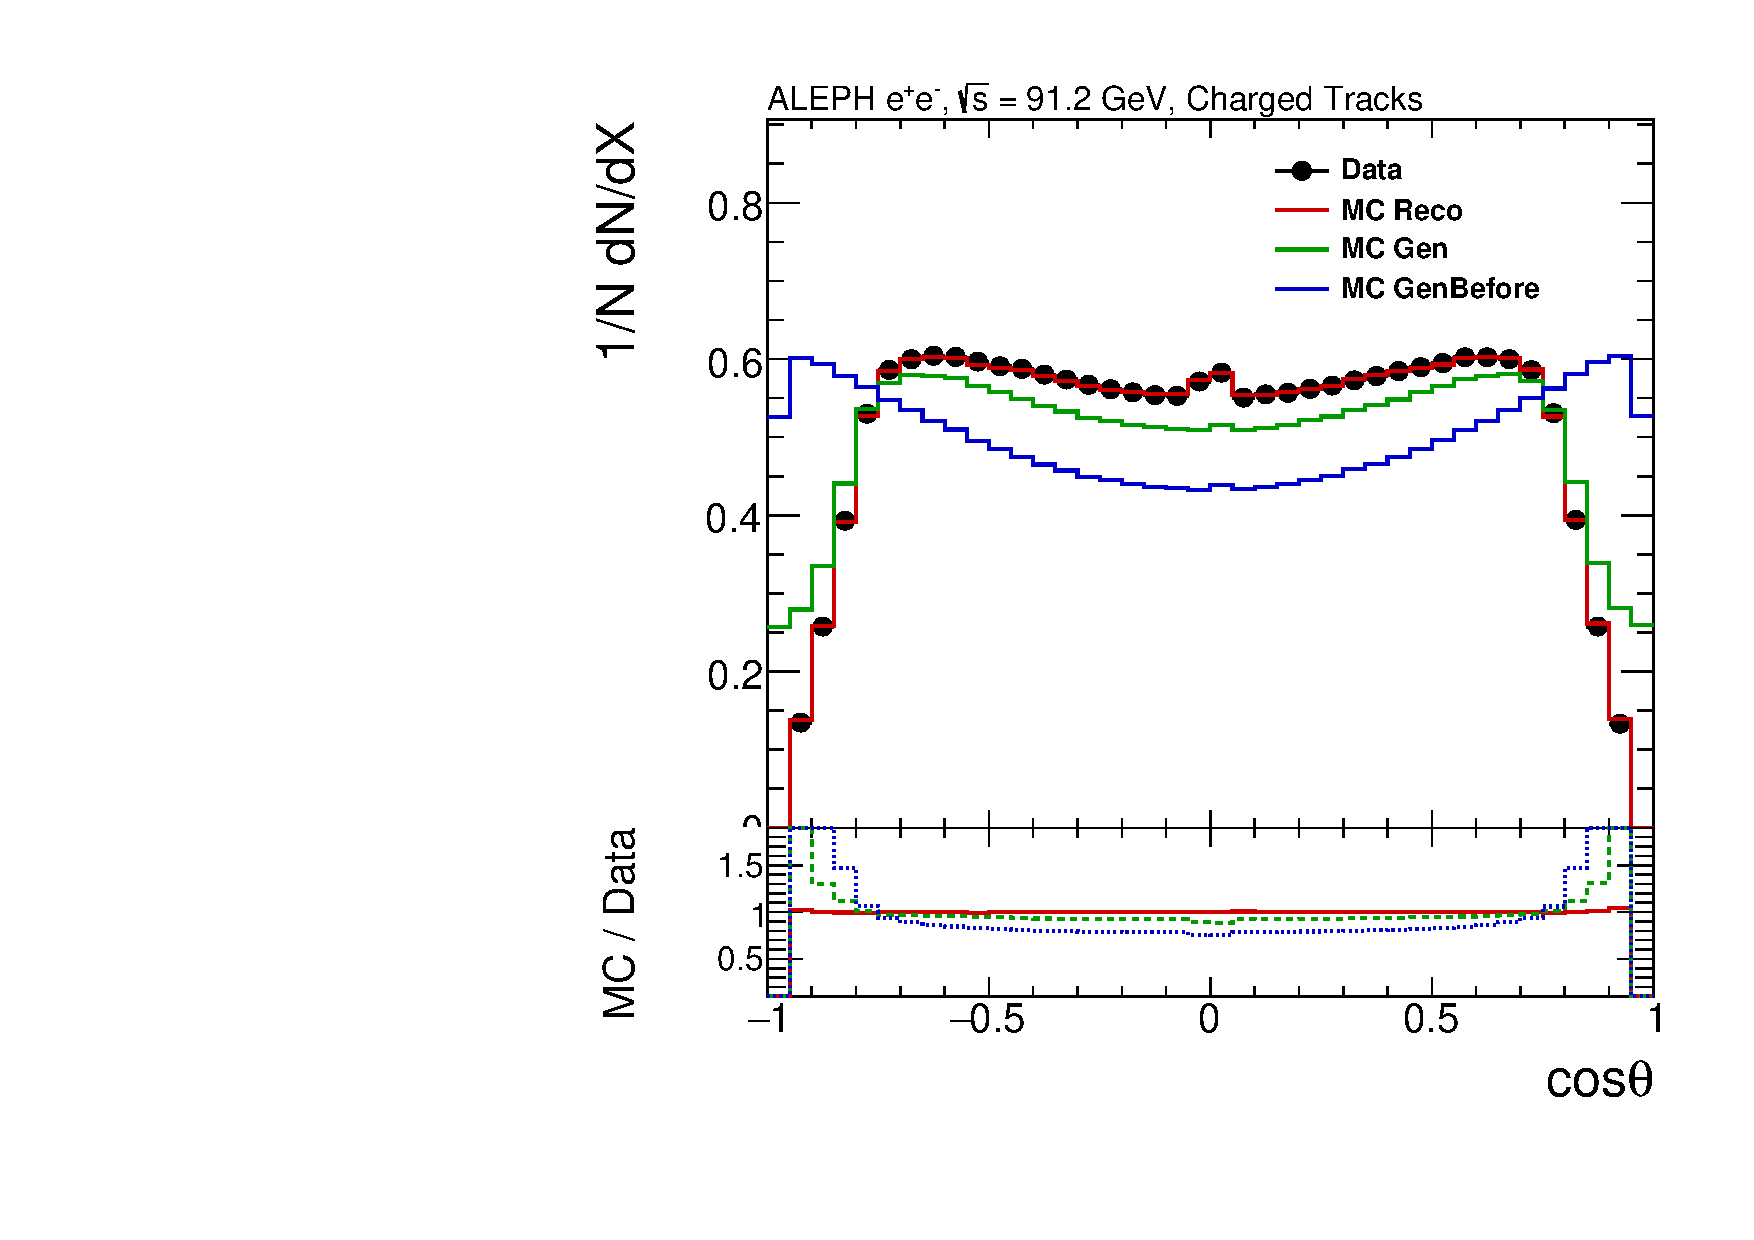
\includegraphics[width=0.325\textwidth]{../Studies/PreliminaryResult/2026-02-17_thrust_iter5/pwflag_kinematics/pwflag0_cosTheta.pdf}
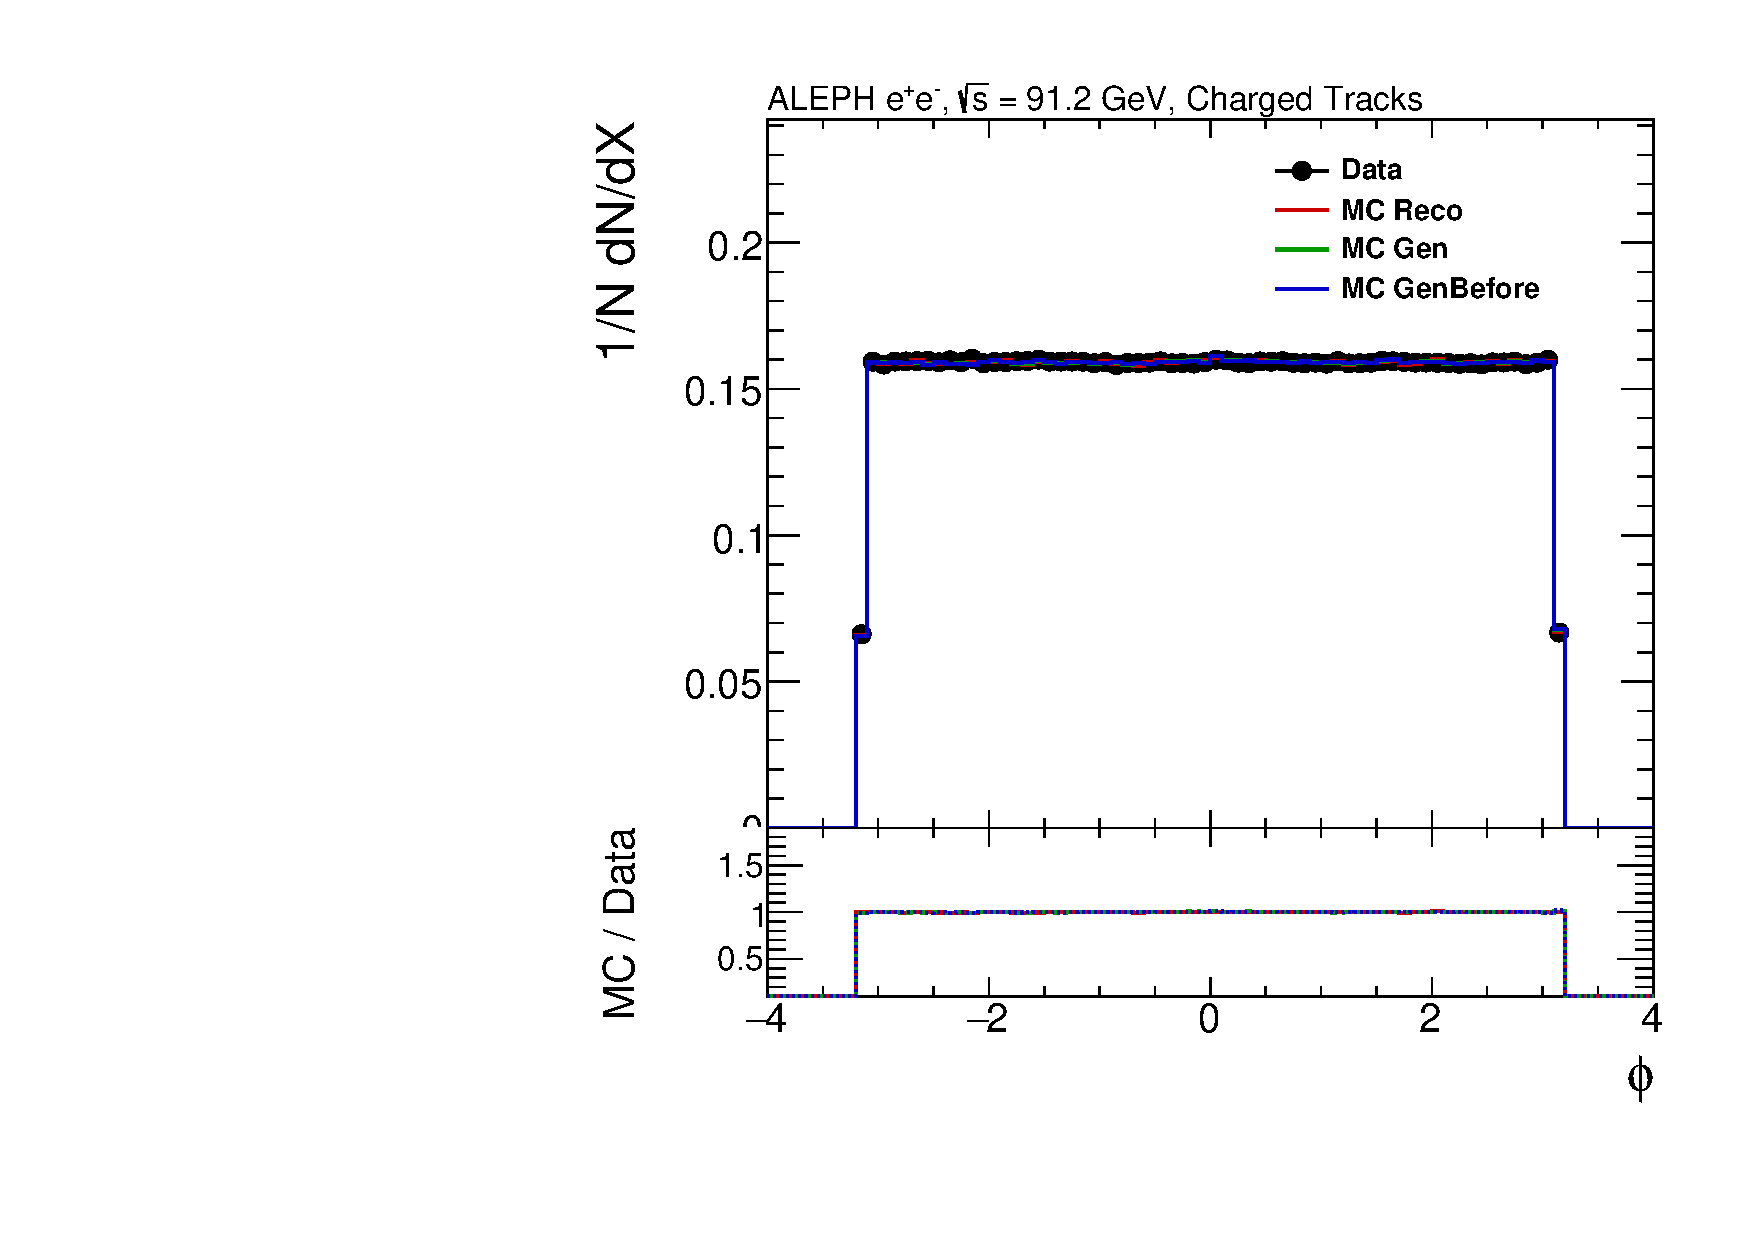
\includegraphics[width=0.325\textwidth]{../Studies/PreliminaryResult/2026-02-17_thrust_iter5/pwflag_kinematics/pwflag0_phi.pdf}
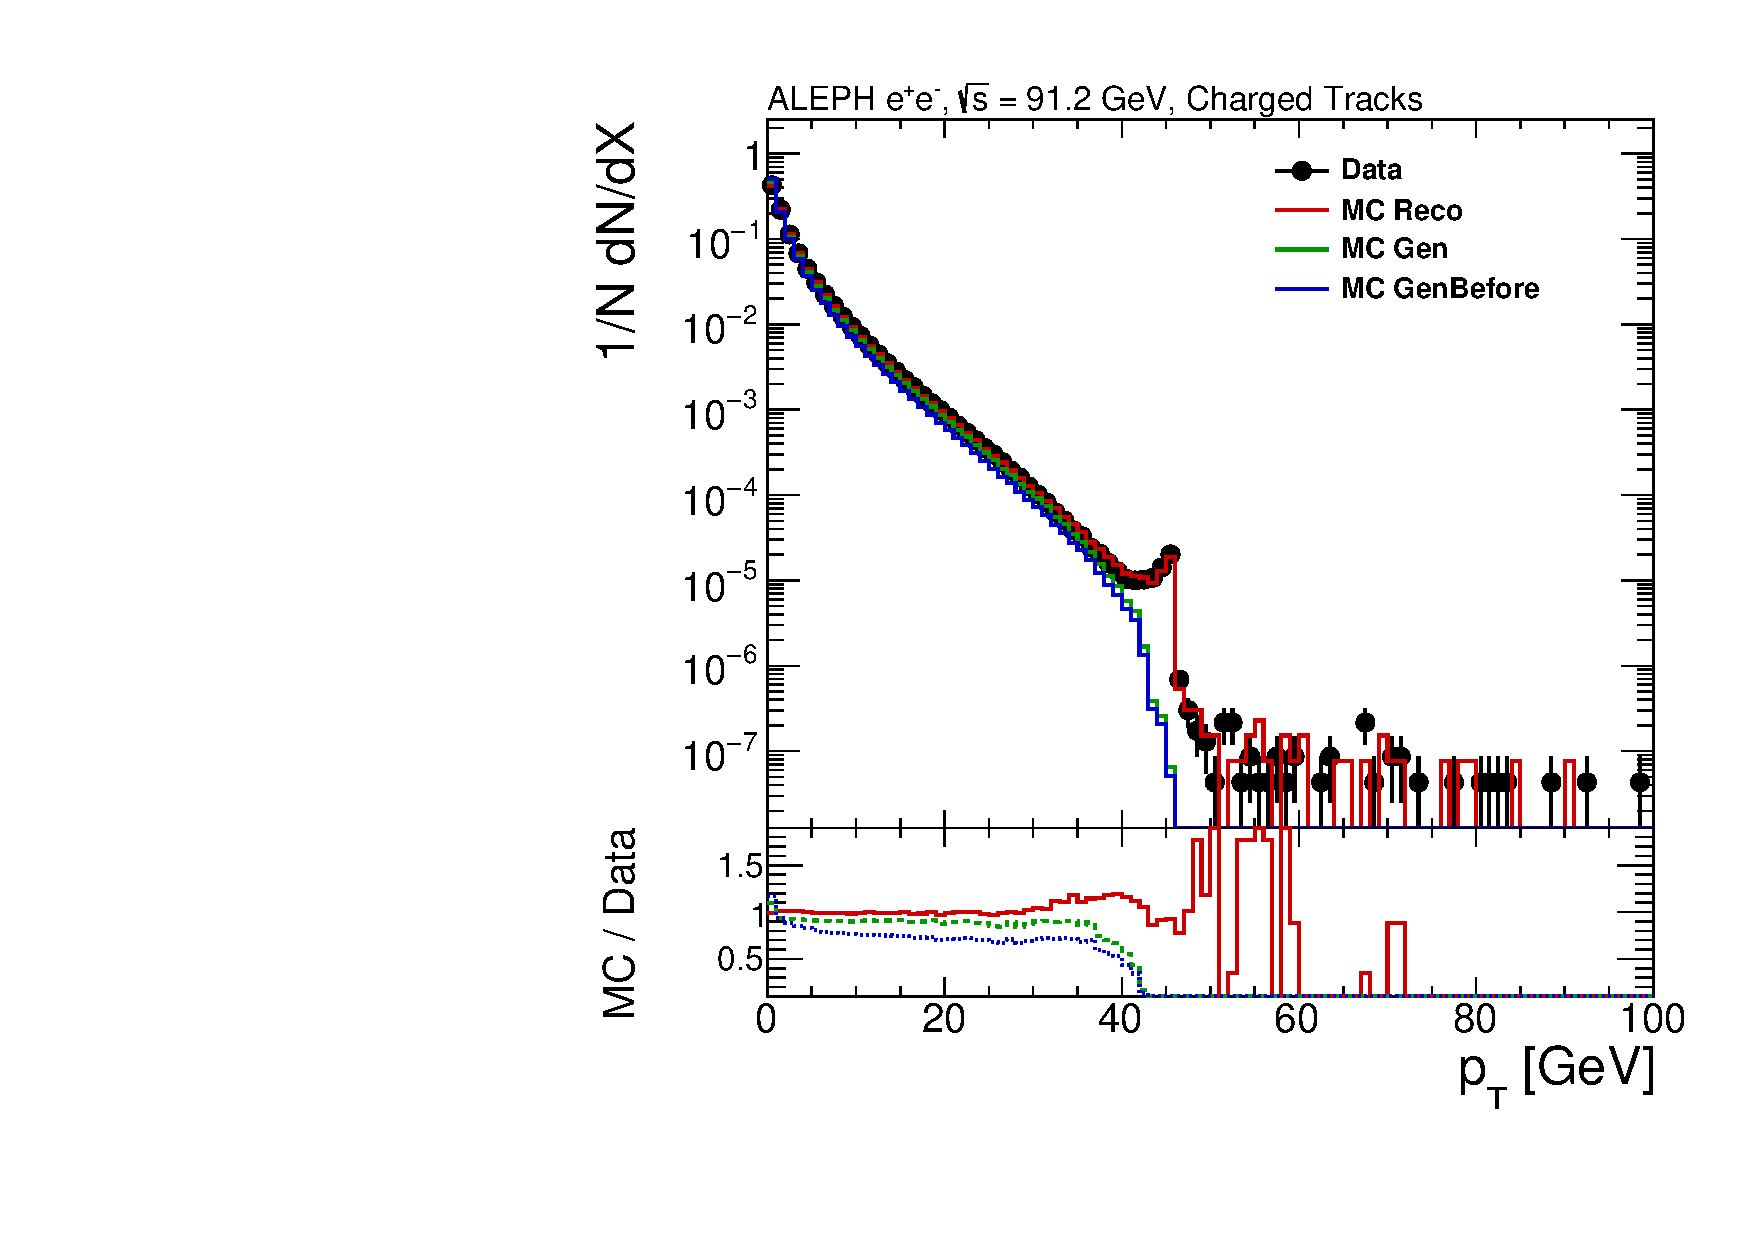
\includegraphics[width=0.325\textwidth]{../Studies/PreliminaryResult/2026-02-17_thrust_iter5/pwflag_kinematics/pwflag0_pt.pdf}
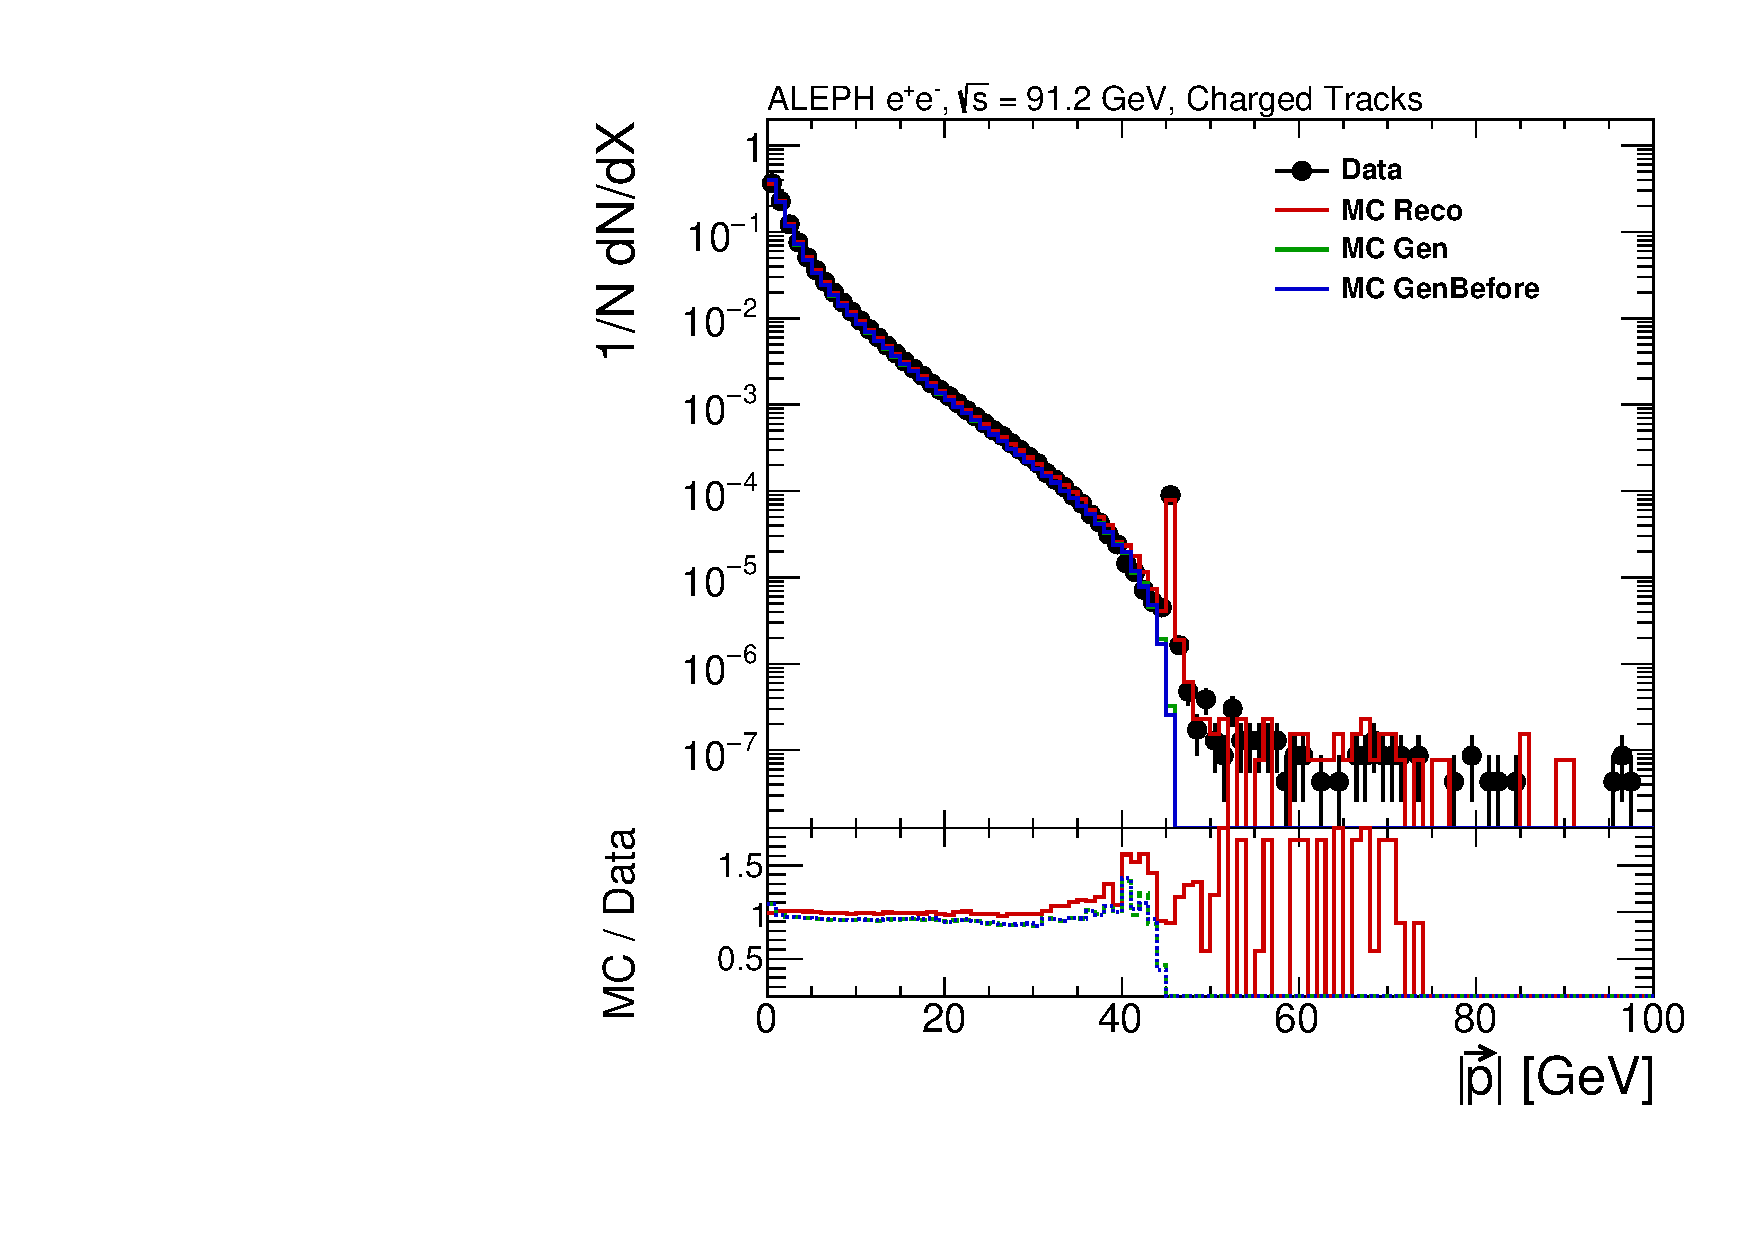
\includegraphics[width=0.325\textwidth]{../Studies/PreliminaryResult/2026-02-17_thrust_iter5/pwflag_kinematics/pwflag0_pmag.pdf}
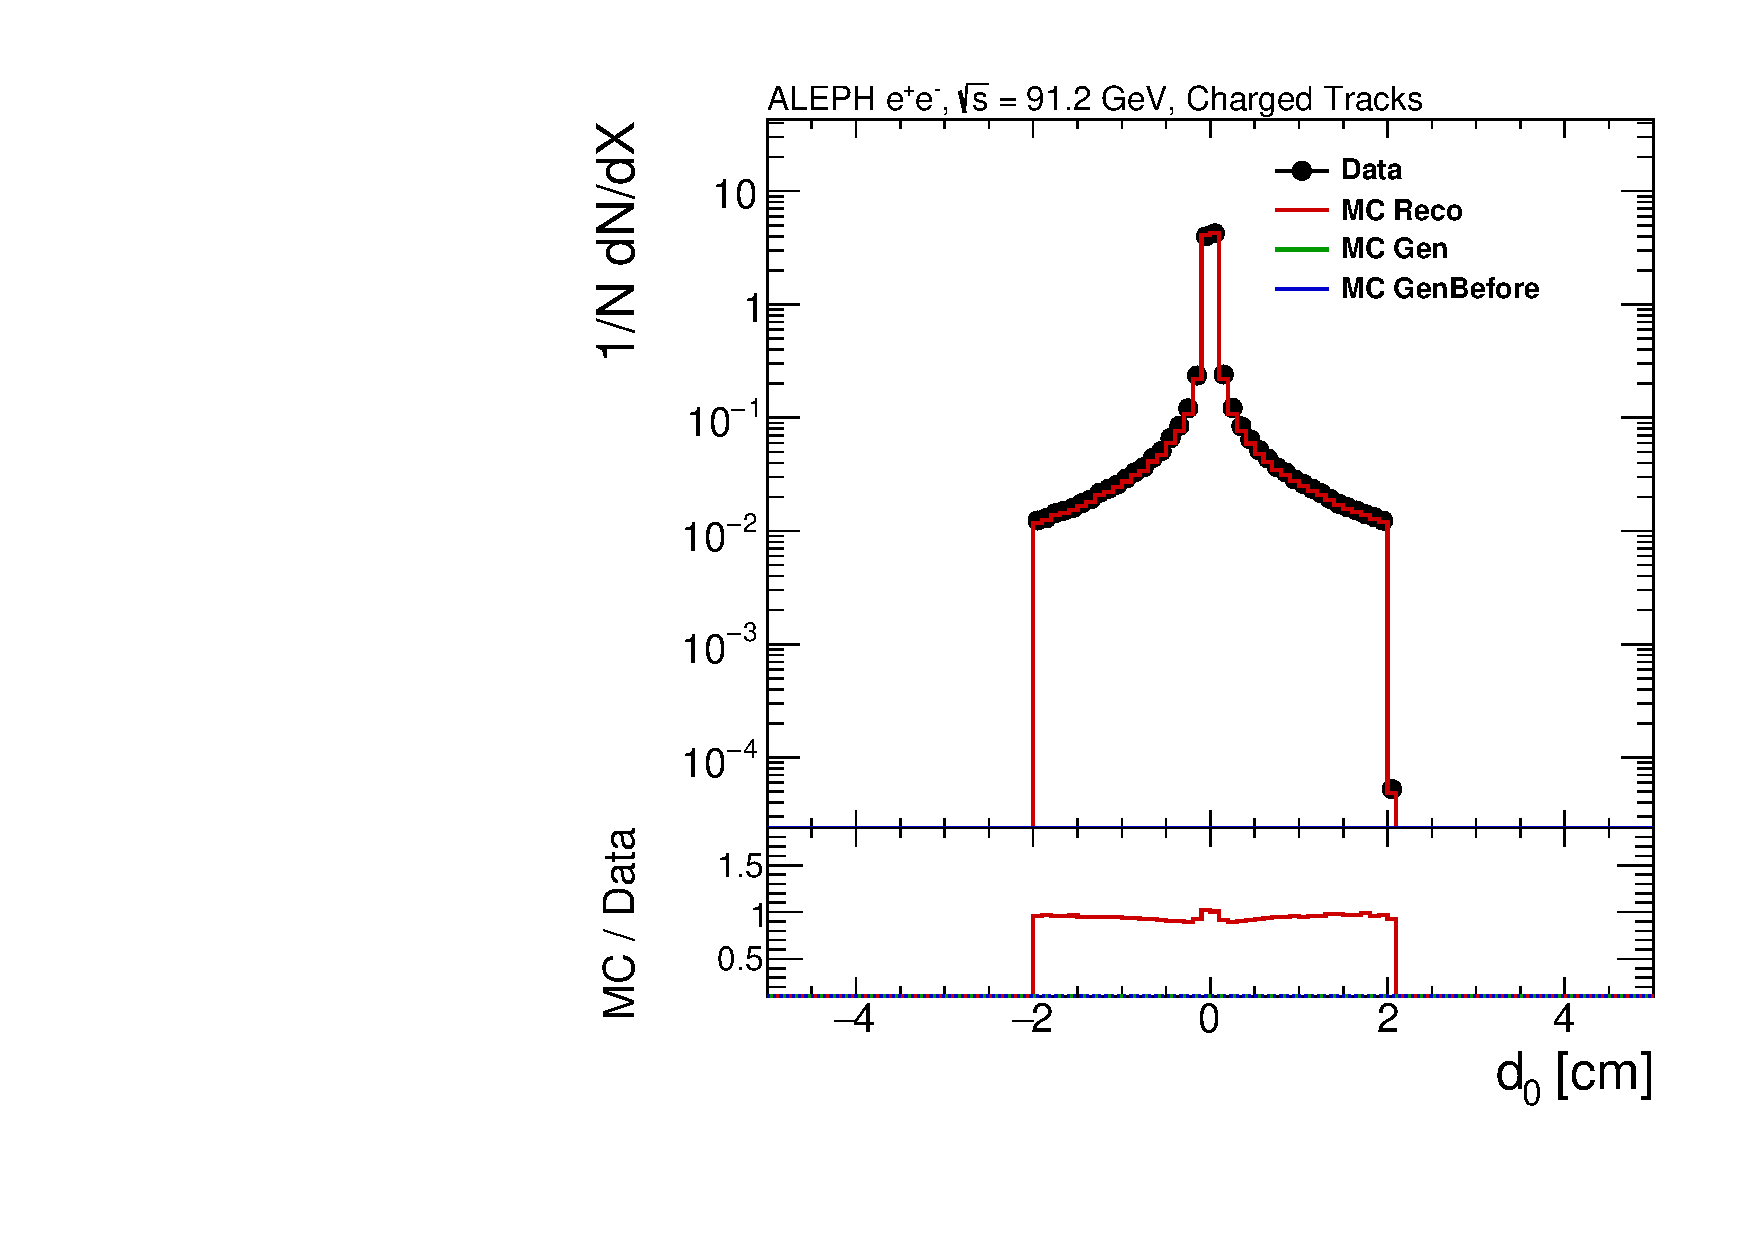
\includegraphics[width=0.325\textwidth]{../Studies/PreliminaryResult/2026-02-17_thrust_iter5/pwflag_kinematics/pwflag0_d0.pdf}
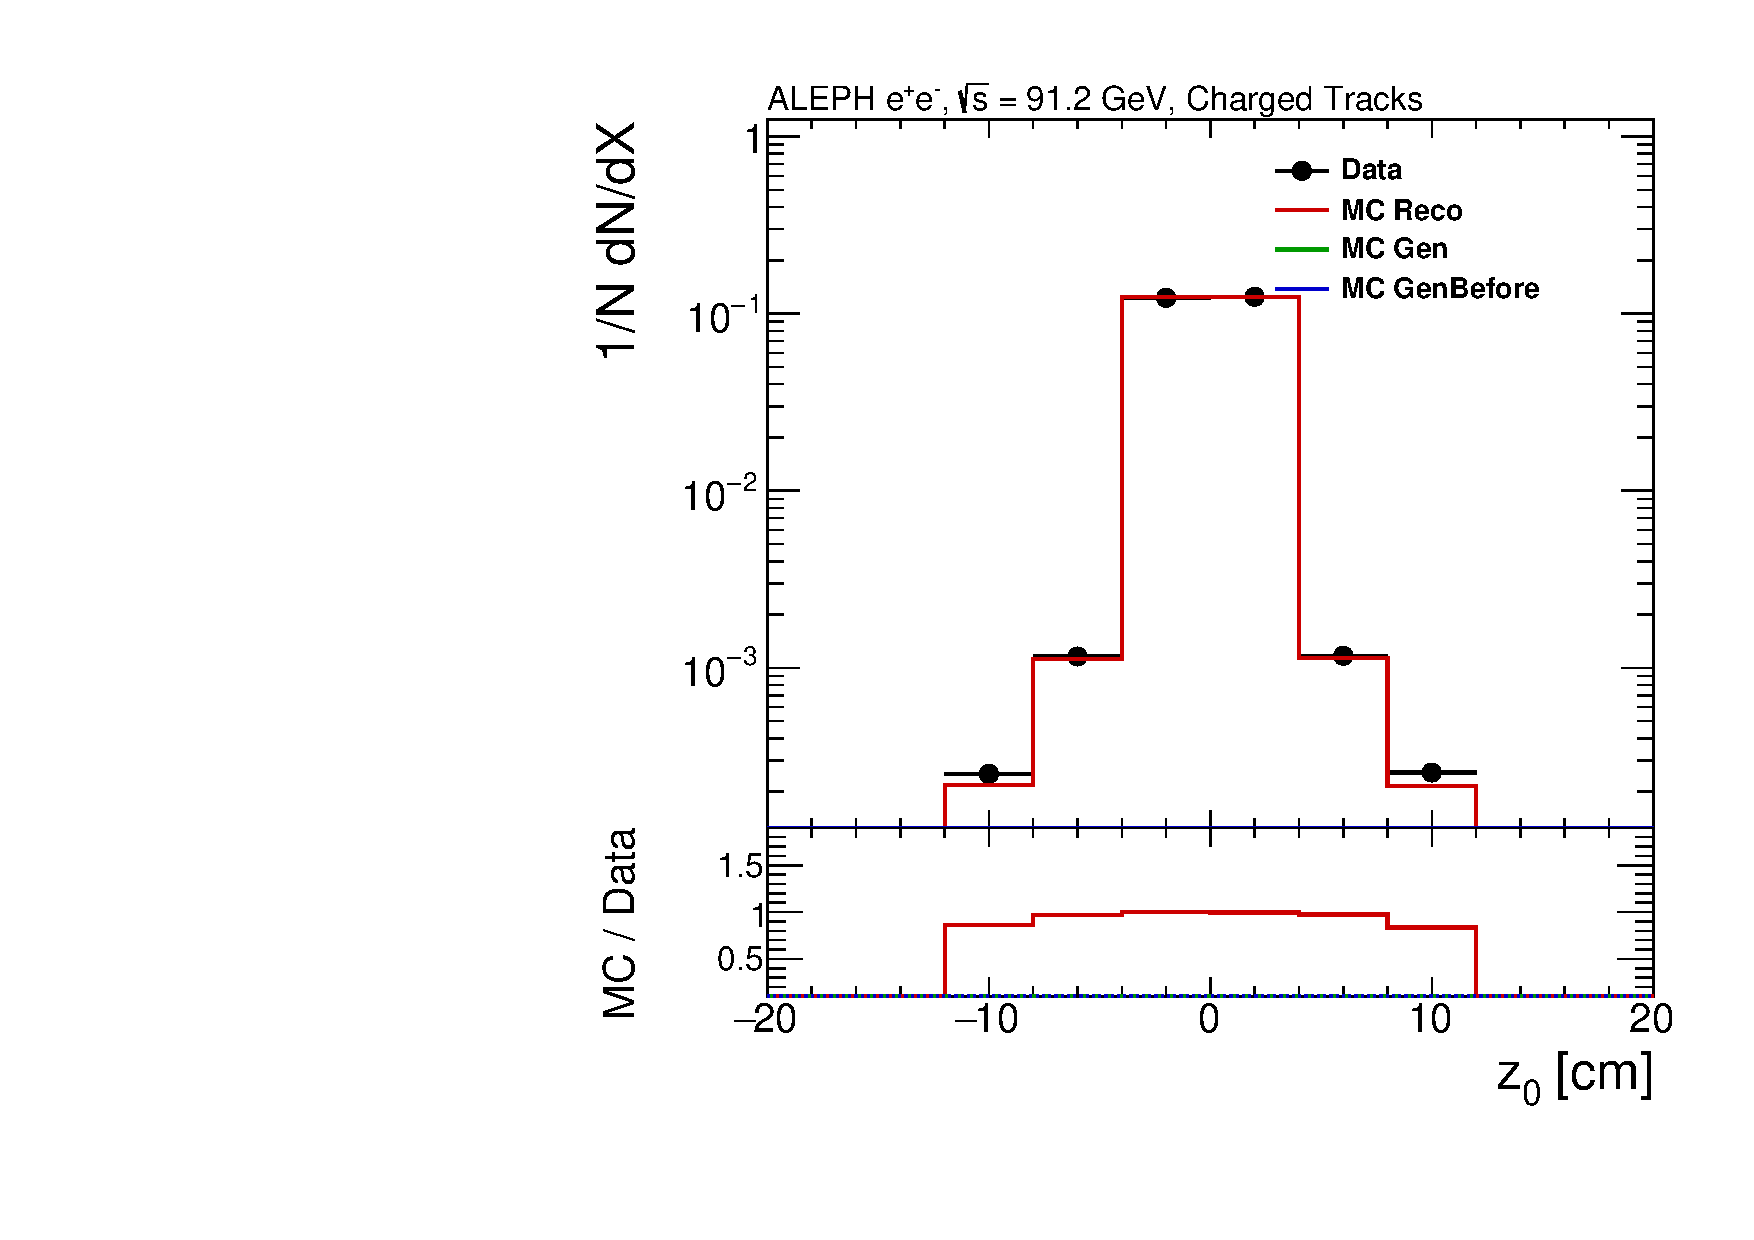
\includegraphics[width=0.325\textwidth]{../Studies/PreliminaryResult/2026-02-17_thrust_iter5/pwflag_kinematics/pwflag0_z0.pdf}
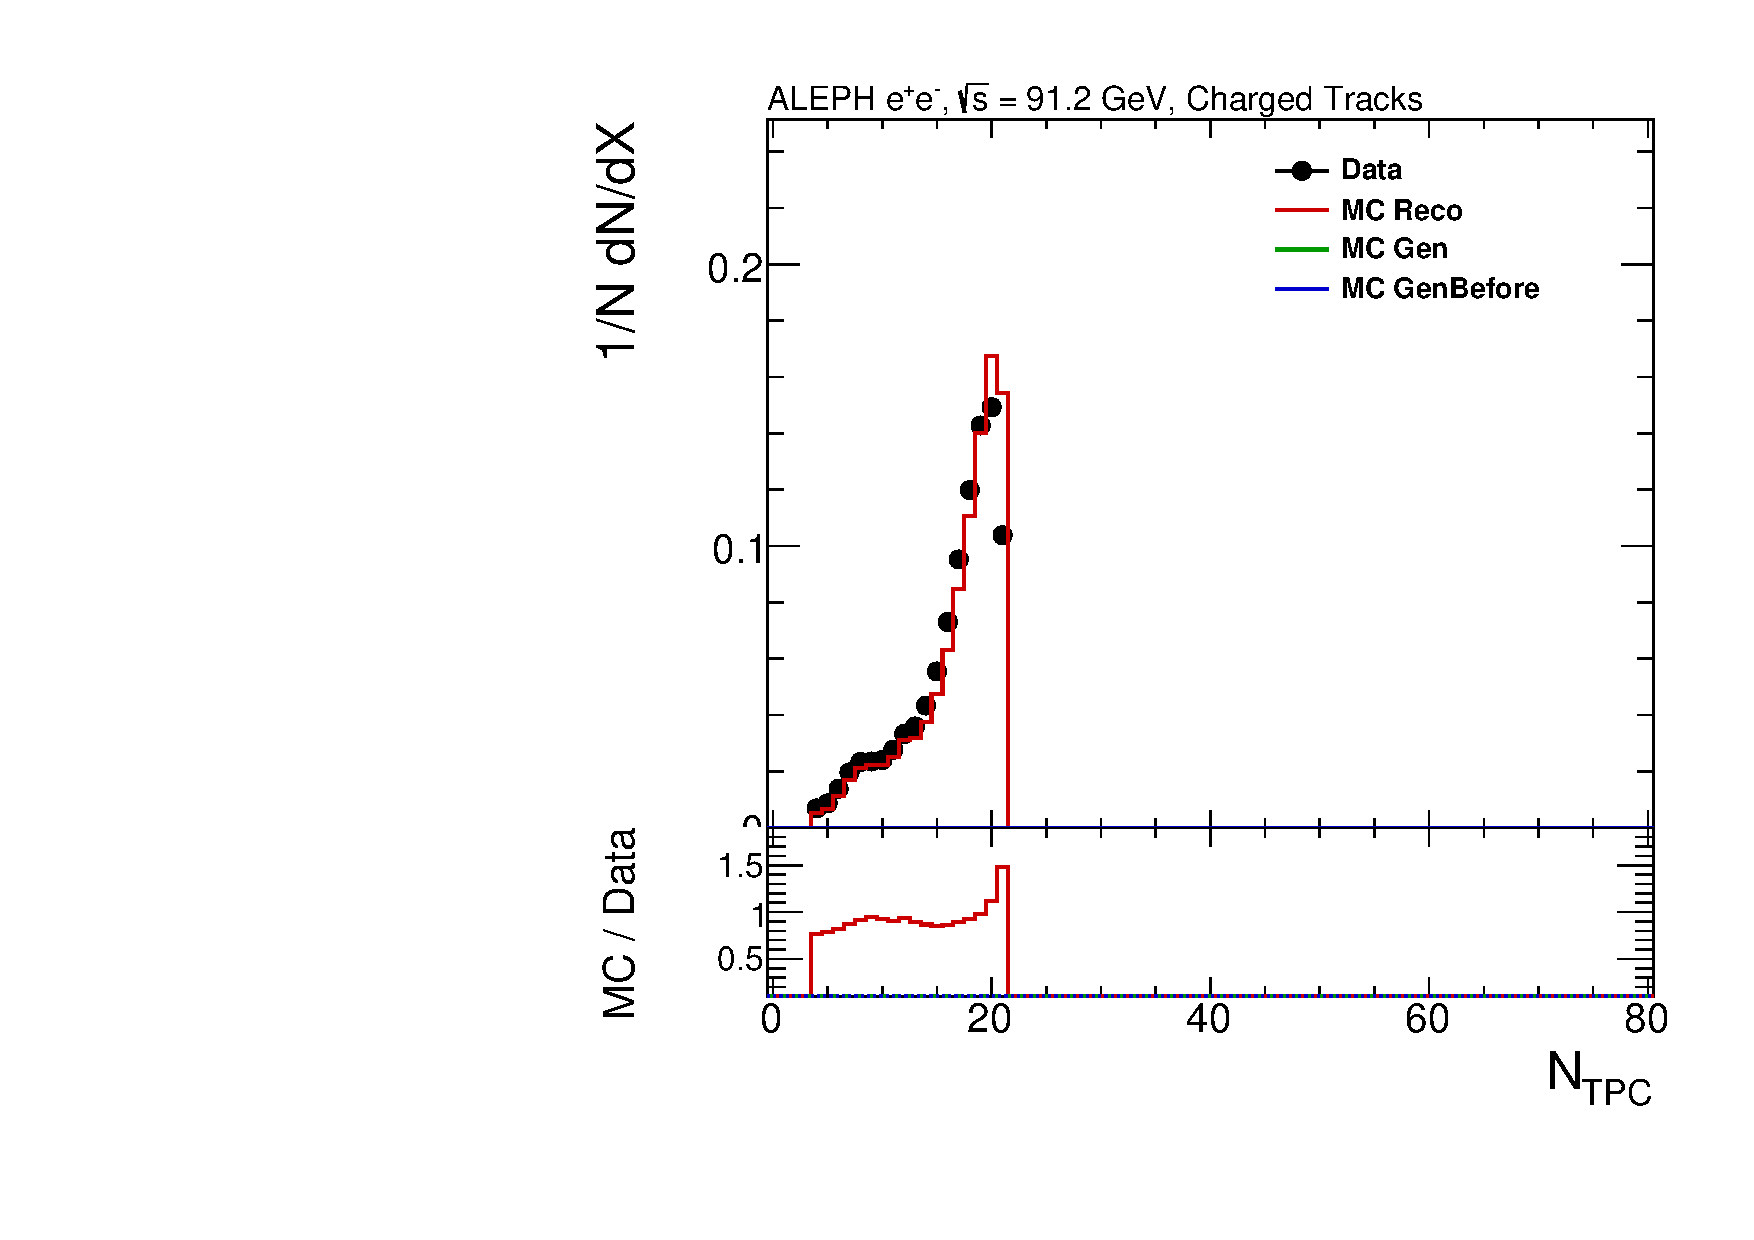
\includegraphics[width=0.325\textwidth]{../Studies/PreliminaryResult/2026-02-17_thrust_iter5/pwflag_kinematics/pwflag0_ntpc.pdf}
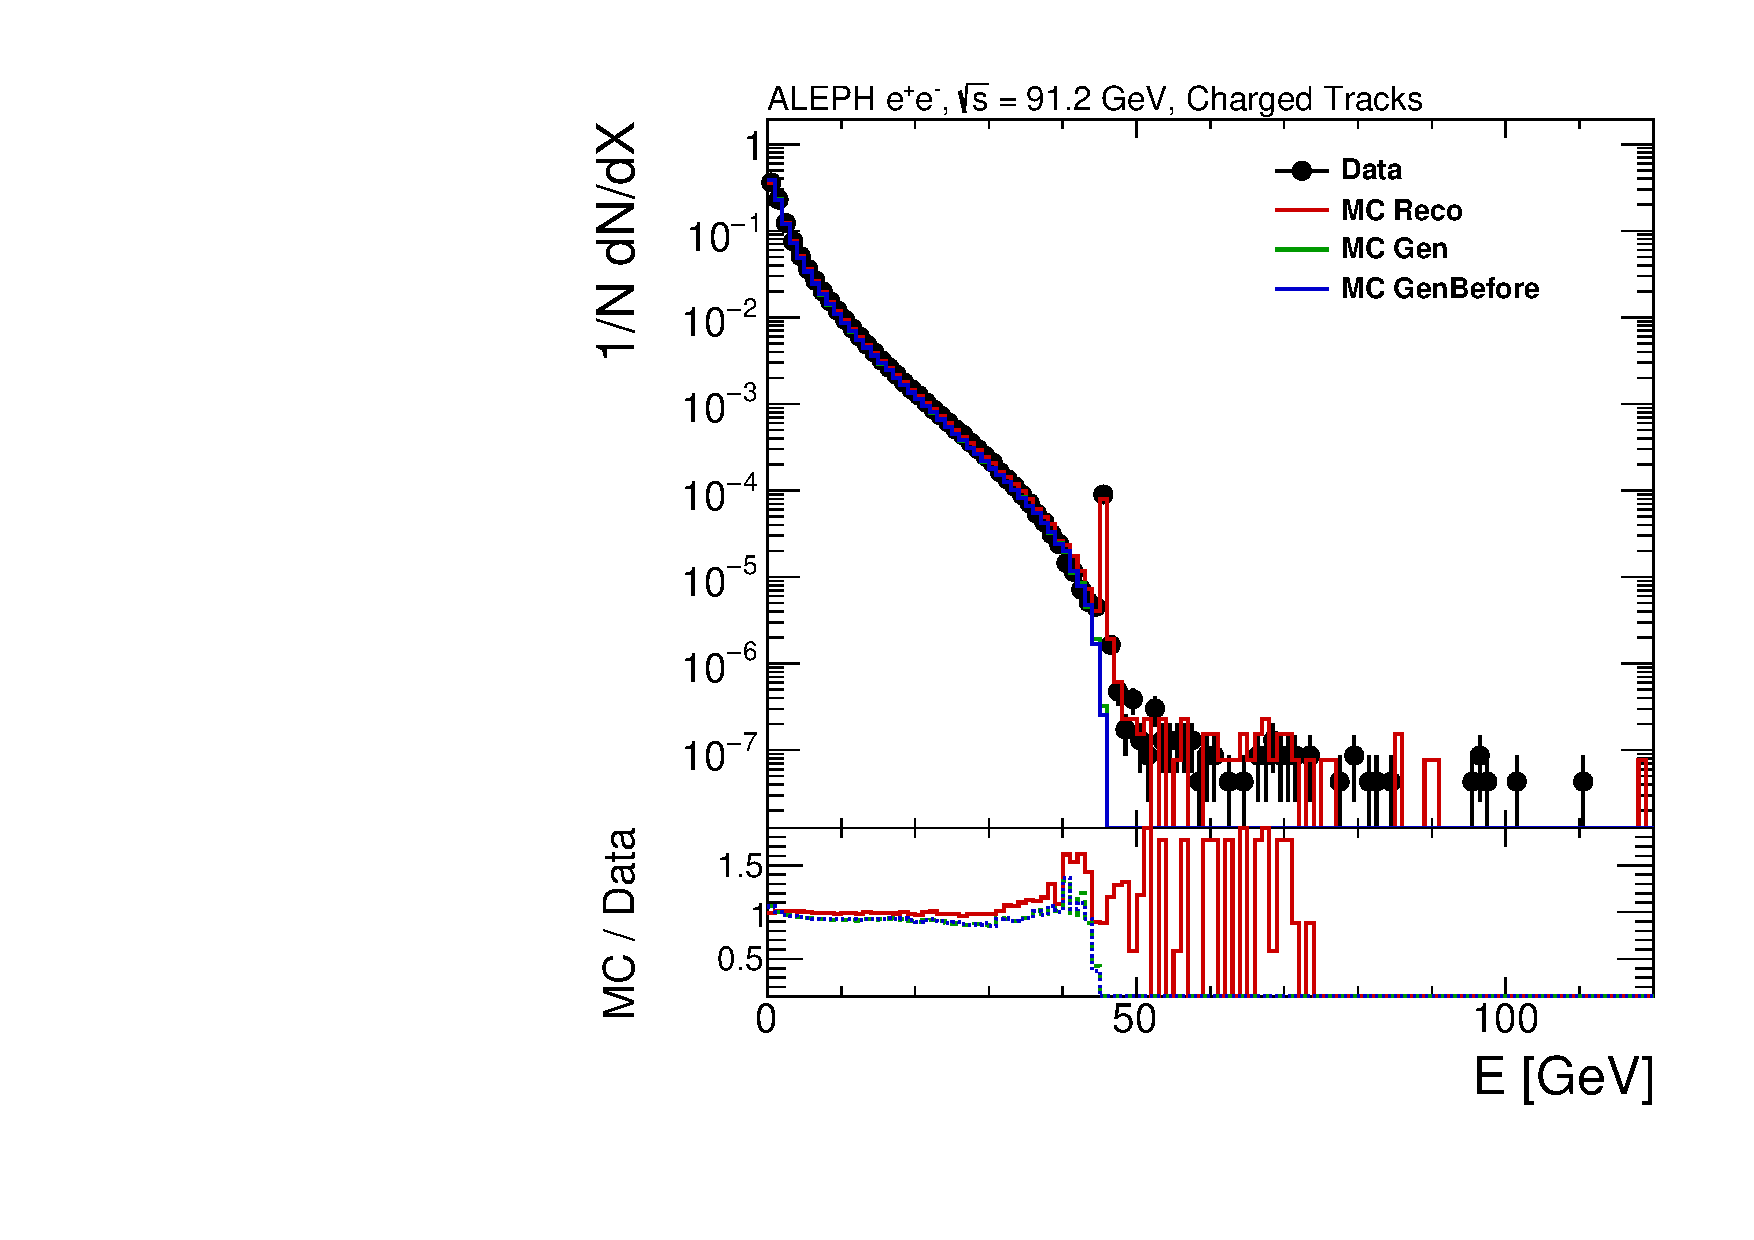
\includegraphics[width=0.325\textwidth]{../Studies/PreliminaryResult/2026-02-17_thrust_iter5/pwflag_kinematics/pwflag0_energy.pdf}
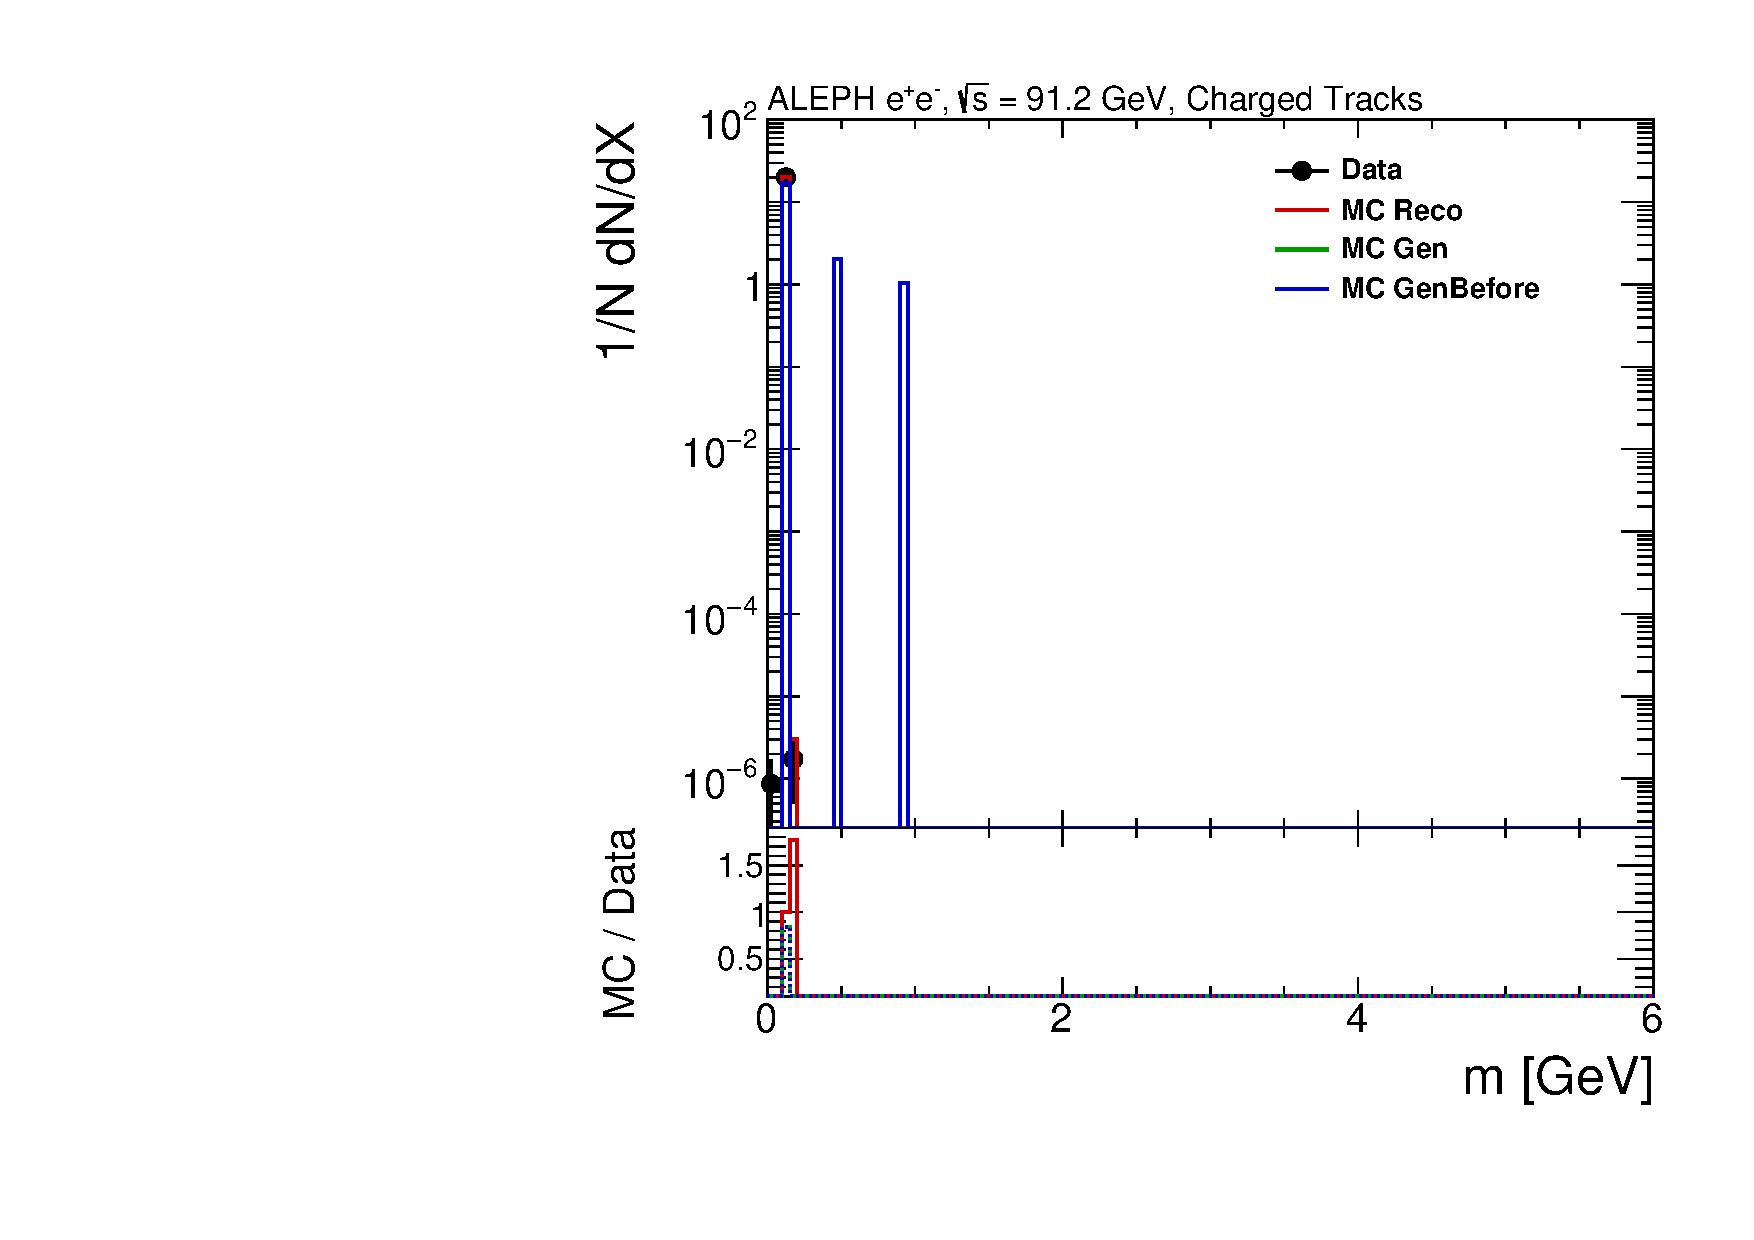
\includegraphics[width=0.325\textwidth]{../Studies/PreliminaryResult/2026-02-17_thrust_iter5/pwflag_kinematics/pwflag0_mass.pdf}
\caption{Complete \texttt{pwflag}=0 kinematic set.}
\label{fig:pwflag0_full}
\end{figure}

\noindent
In Fig.~\ref{fig:pwflag0_full}, the charged-track category drives the event-shape denominator
and axis finding, so agreement here anchors the full detector response modeling. The
$\cos\theta$ distribution shows the expected enhancement away from the acceptance edges and a
falloff near the fiducial boundary, while the $d_0$ and $z_0$ spectra are concentrated in the
high-quality track region selected for the nominal sample. The $N_{\mathrm{TPC}}$, $p_T$, and
energy panels provide direct checks that tracking-quality and hard-track tails are described with
the precision required for stable thrust unfolding.

\begin{figure}[t!]
\centering
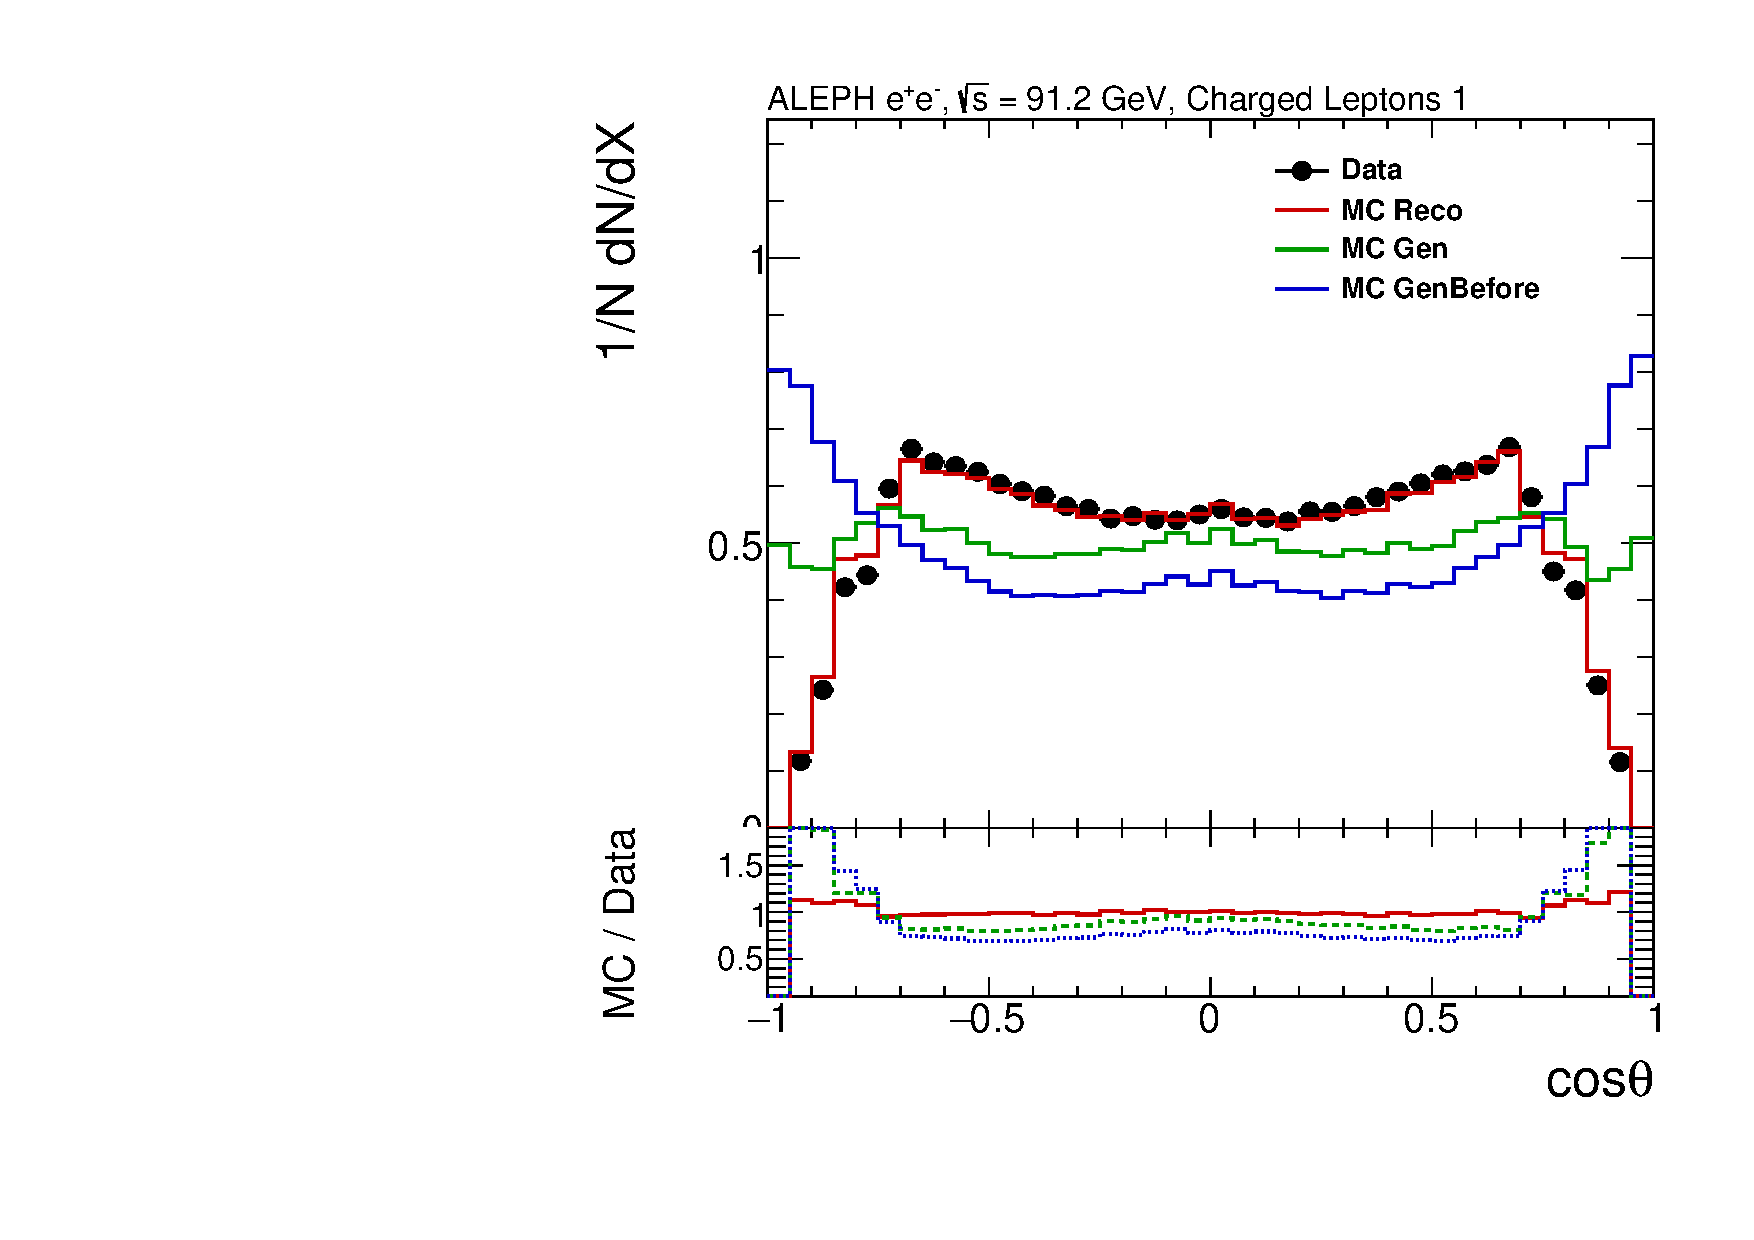
\includegraphics[width=0.325\textwidth]{../Studies/PreliminaryResult/2026-02-17_thrust_iter5/pwflag_kinematics/pwflag1_cosTheta.pdf}
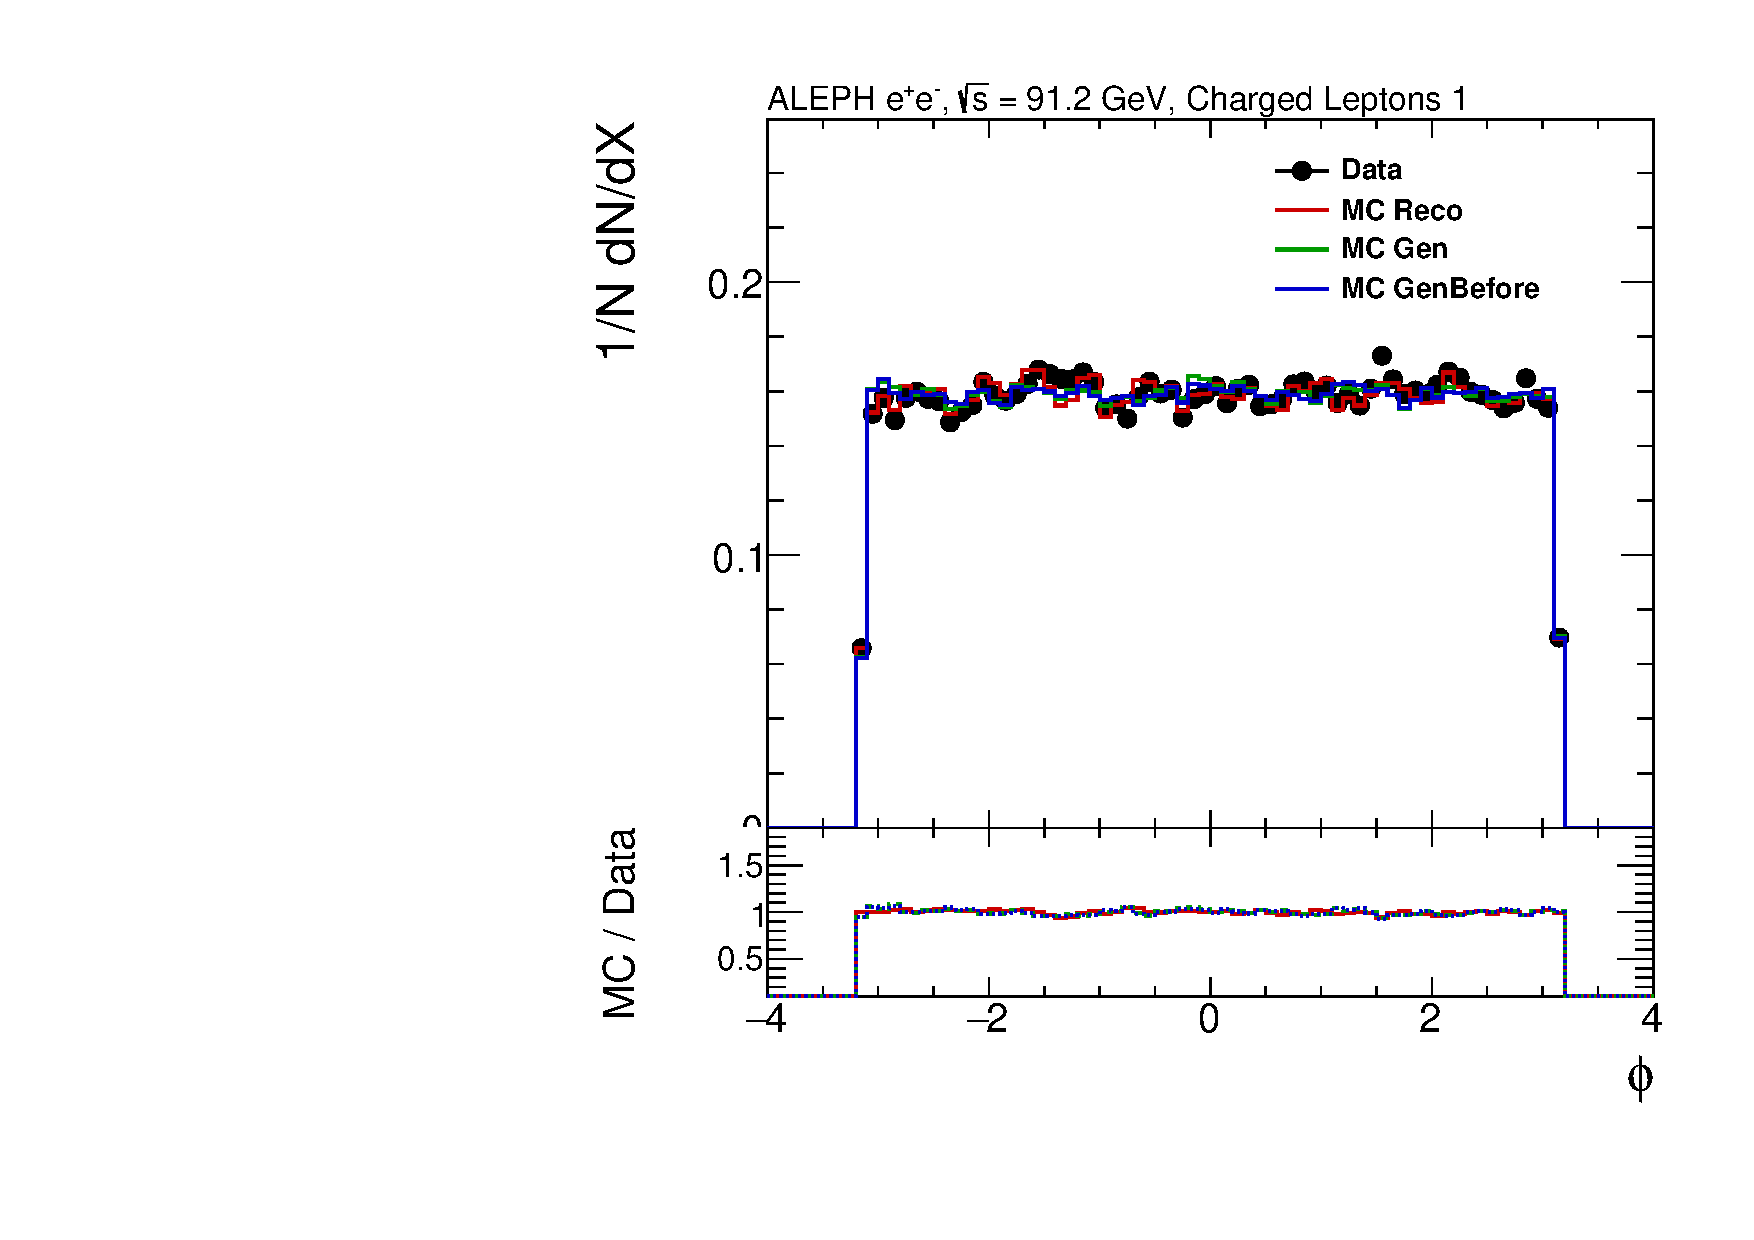
\includegraphics[width=0.325\textwidth]{../Studies/PreliminaryResult/2026-02-17_thrust_iter5/pwflag_kinematics/pwflag1_phi.pdf}
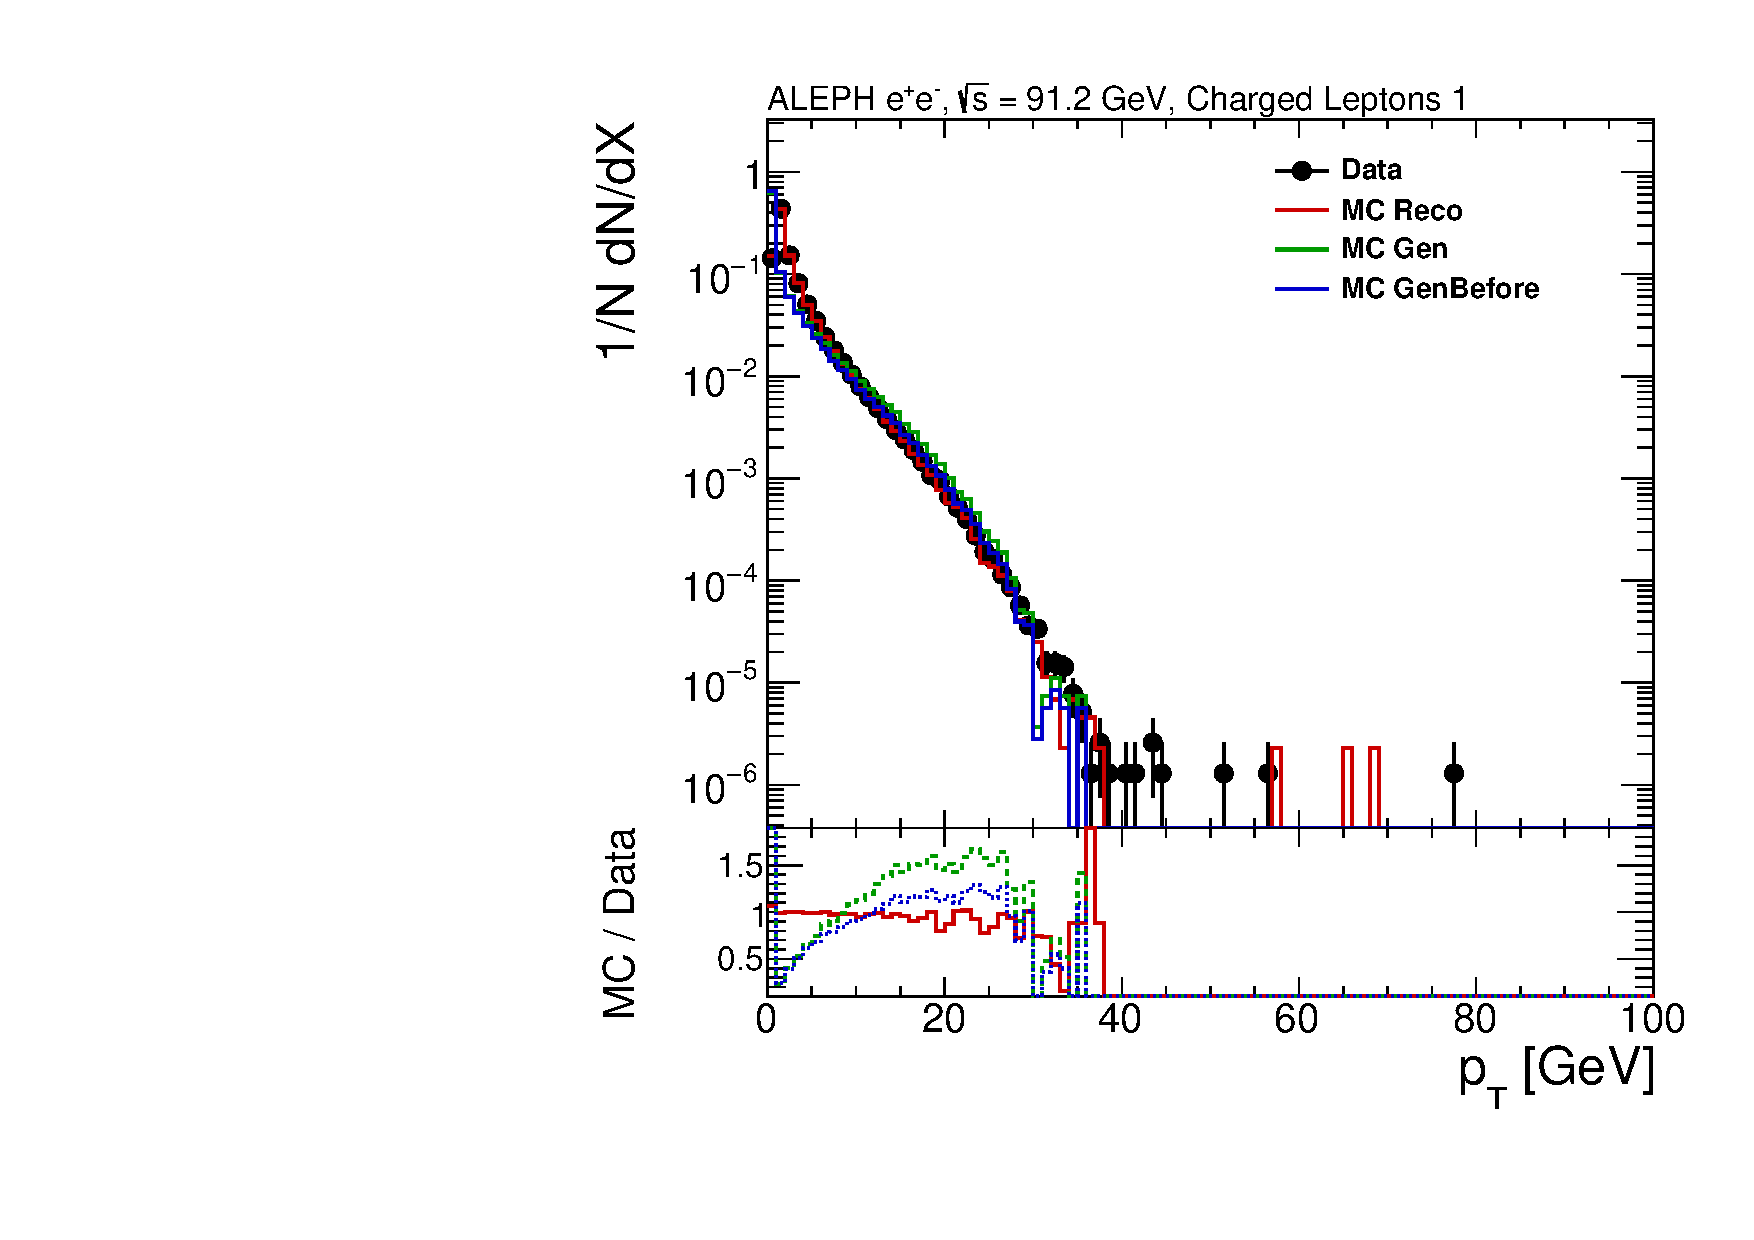
\includegraphics[width=0.325\textwidth]{../Studies/PreliminaryResult/2026-02-17_thrust_iter5/pwflag_kinematics/pwflag1_pt.pdf}
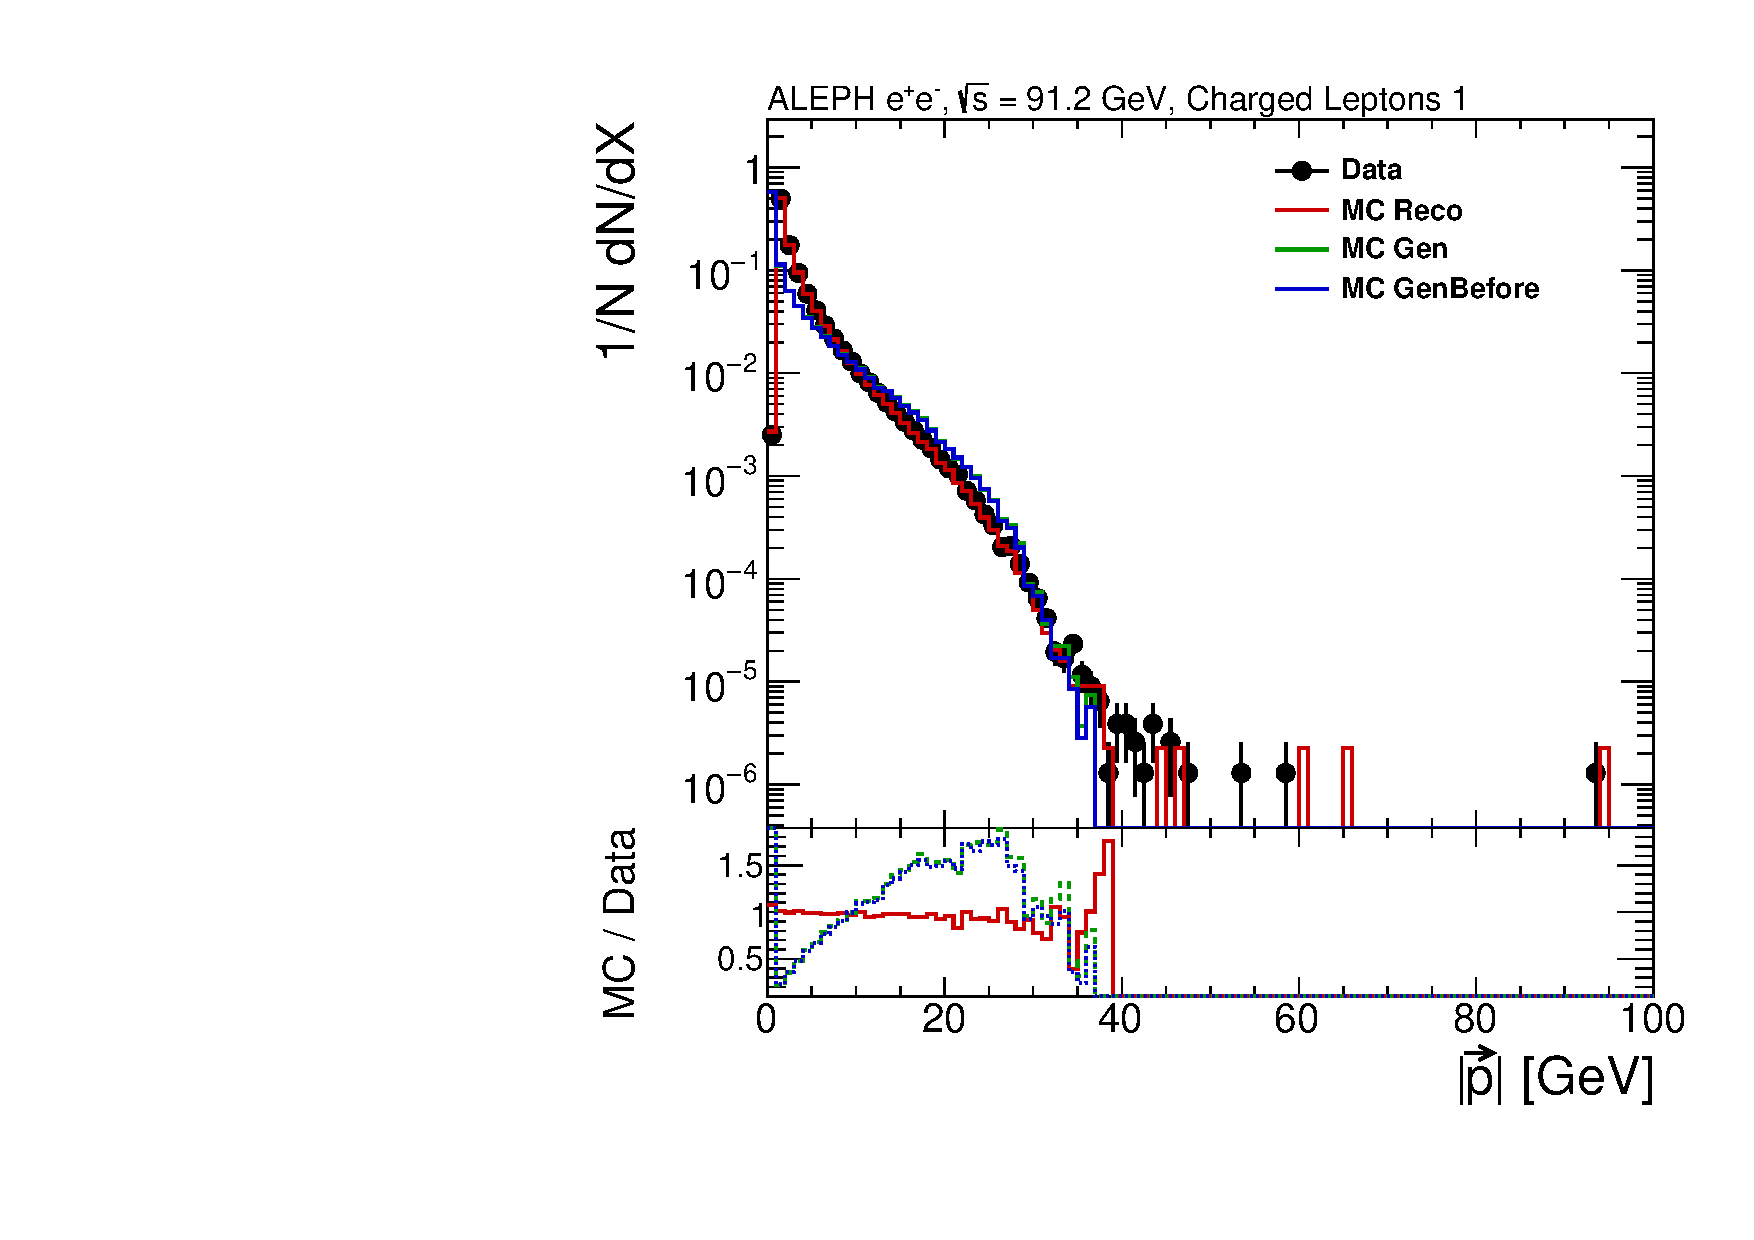
\includegraphics[width=0.325\textwidth]{../Studies/PreliminaryResult/2026-02-17_thrust_iter5/pwflag_kinematics/pwflag1_pmag.pdf}
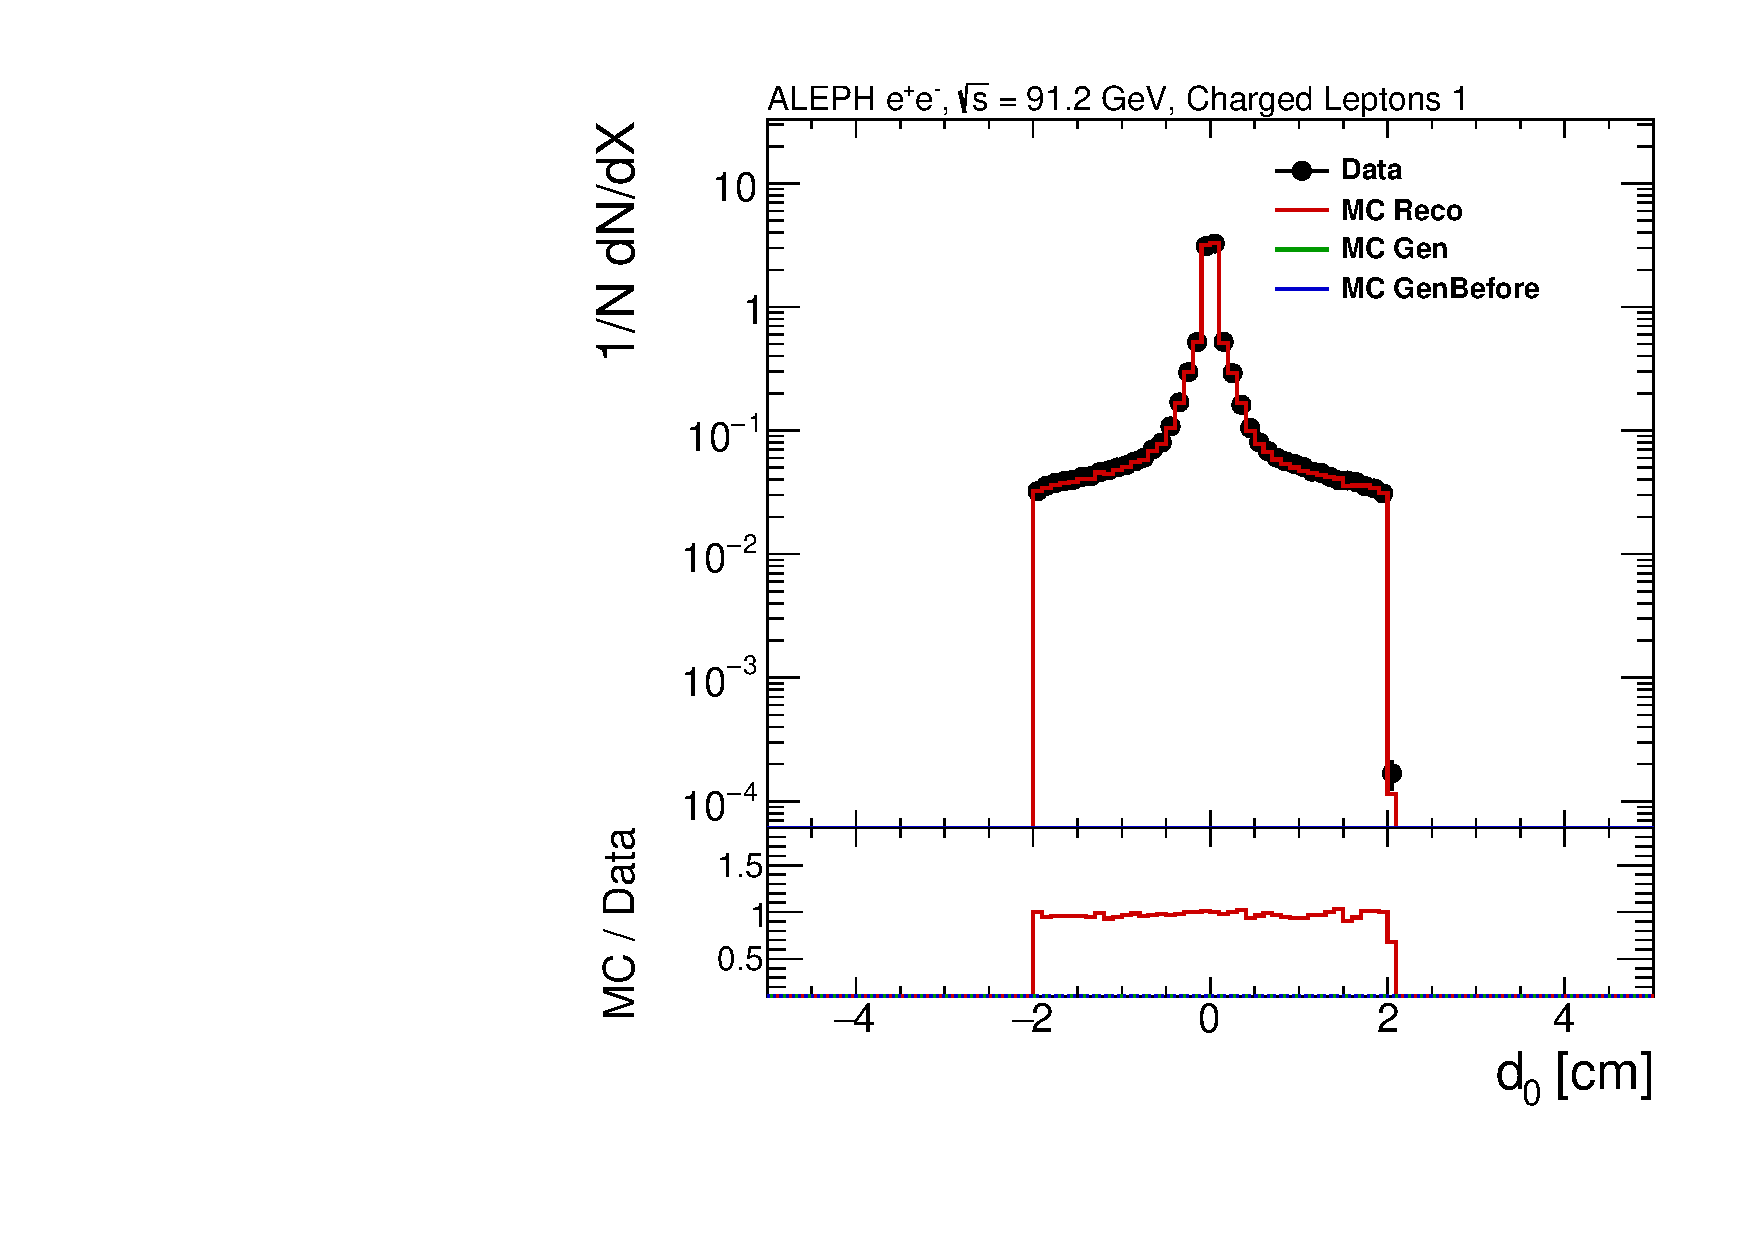
\includegraphics[width=0.325\textwidth]{../Studies/PreliminaryResult/2026-02-17_thrust_iter5/pwflag_kinematics/pwflag1_d0.pdf}
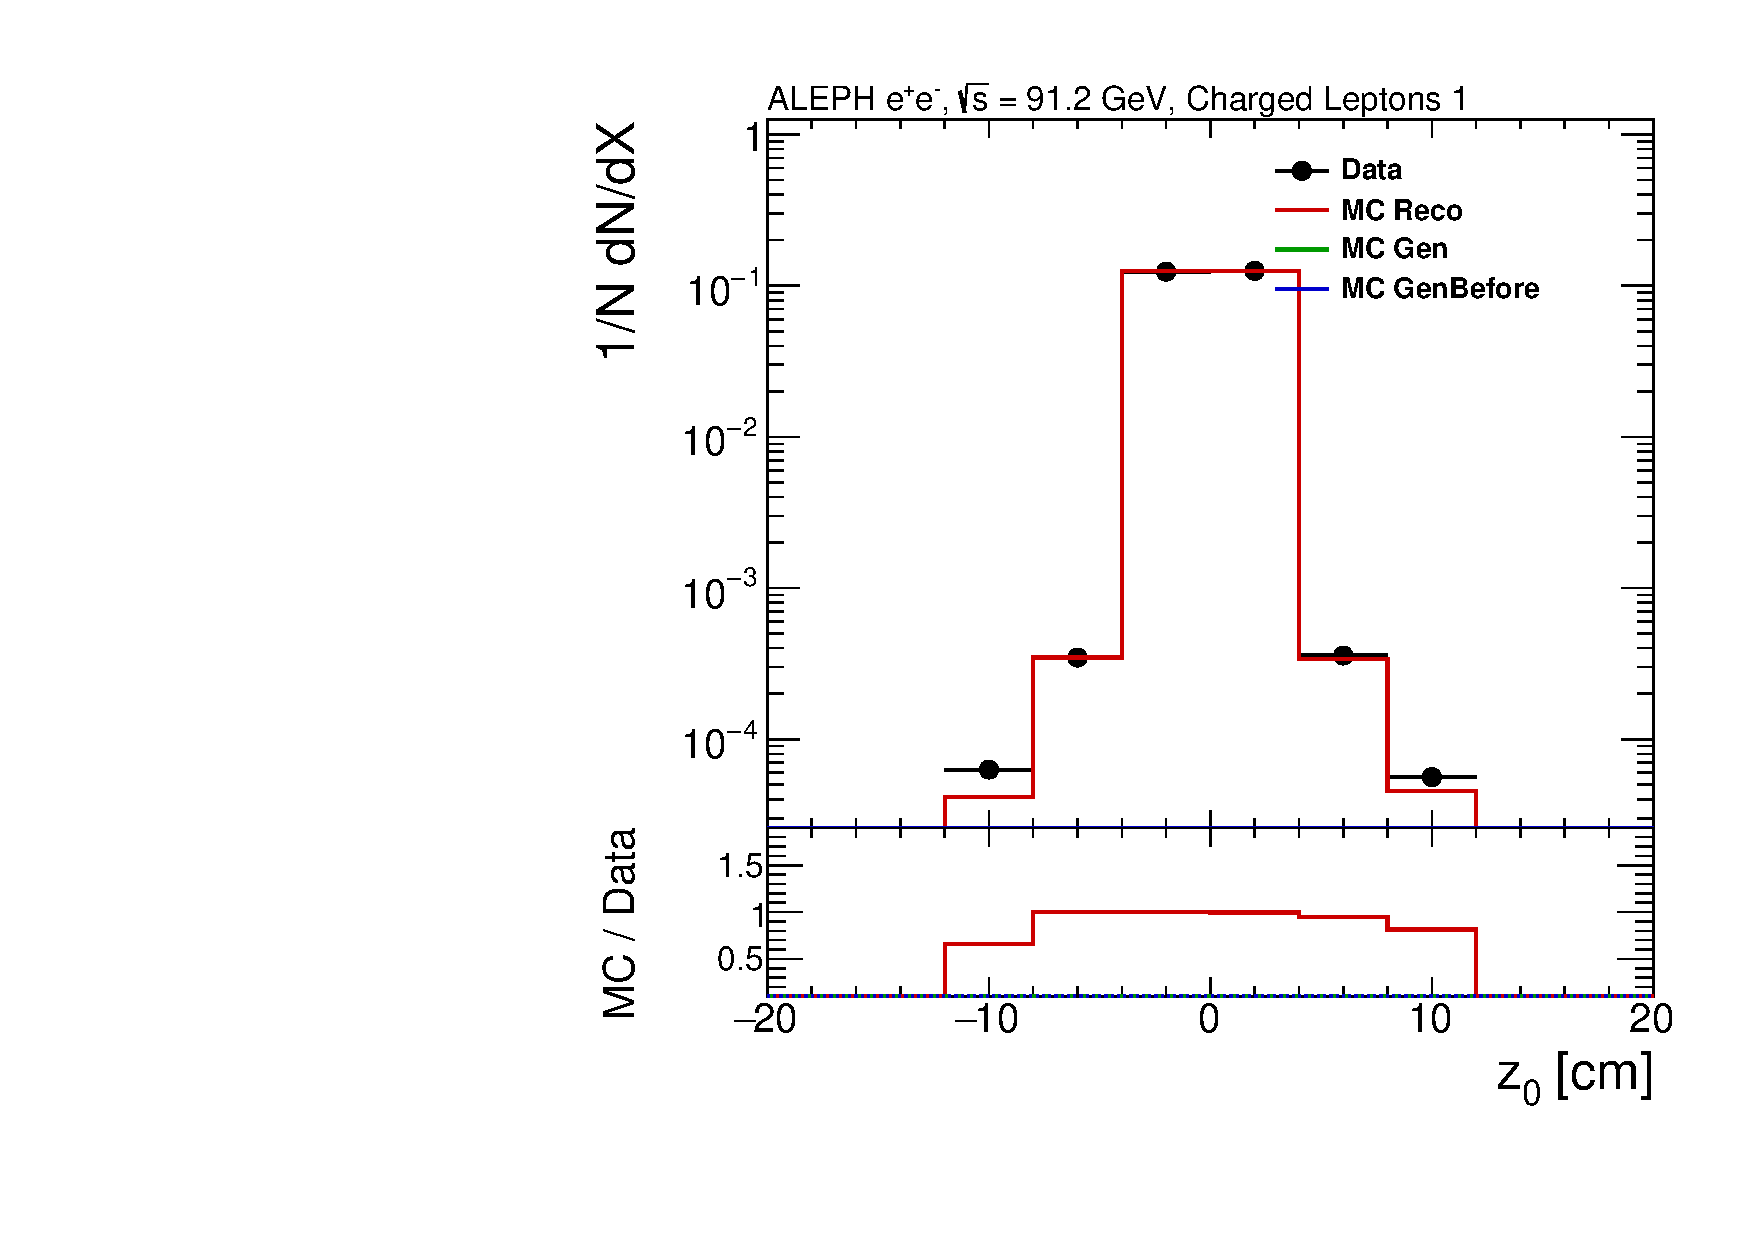
\includegraphics[width=0.325\textwidth]{../Studies/PreliminaryResult/2026-02-17_thrust_iter5/pwflag_kinematics/pwflag1_z0.pdf}
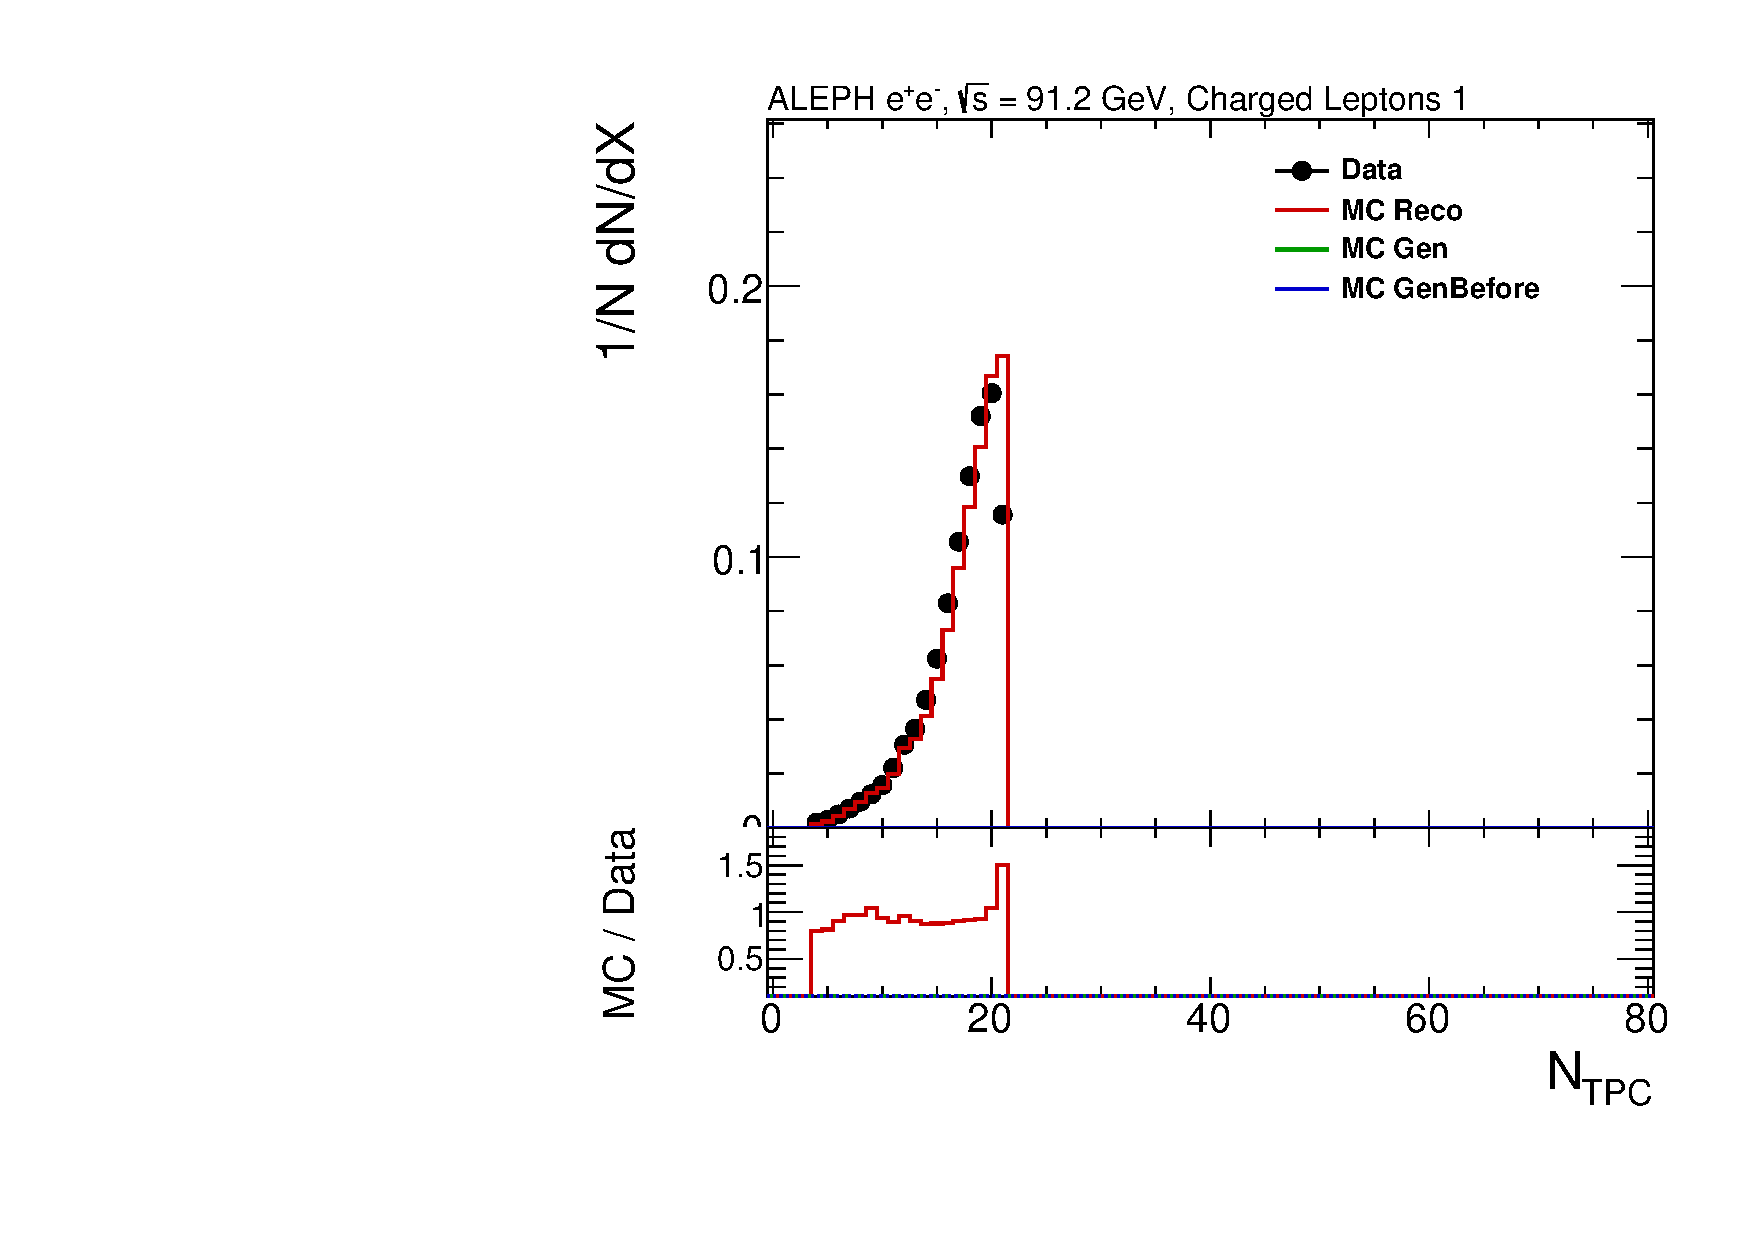
\includegraphics[width=0.325\textwidth]{../Studies/PreliminaryResult/2026-02-17_thrust_iter5/pwflag_kinematics/pwflag1_ntpc.pdf}
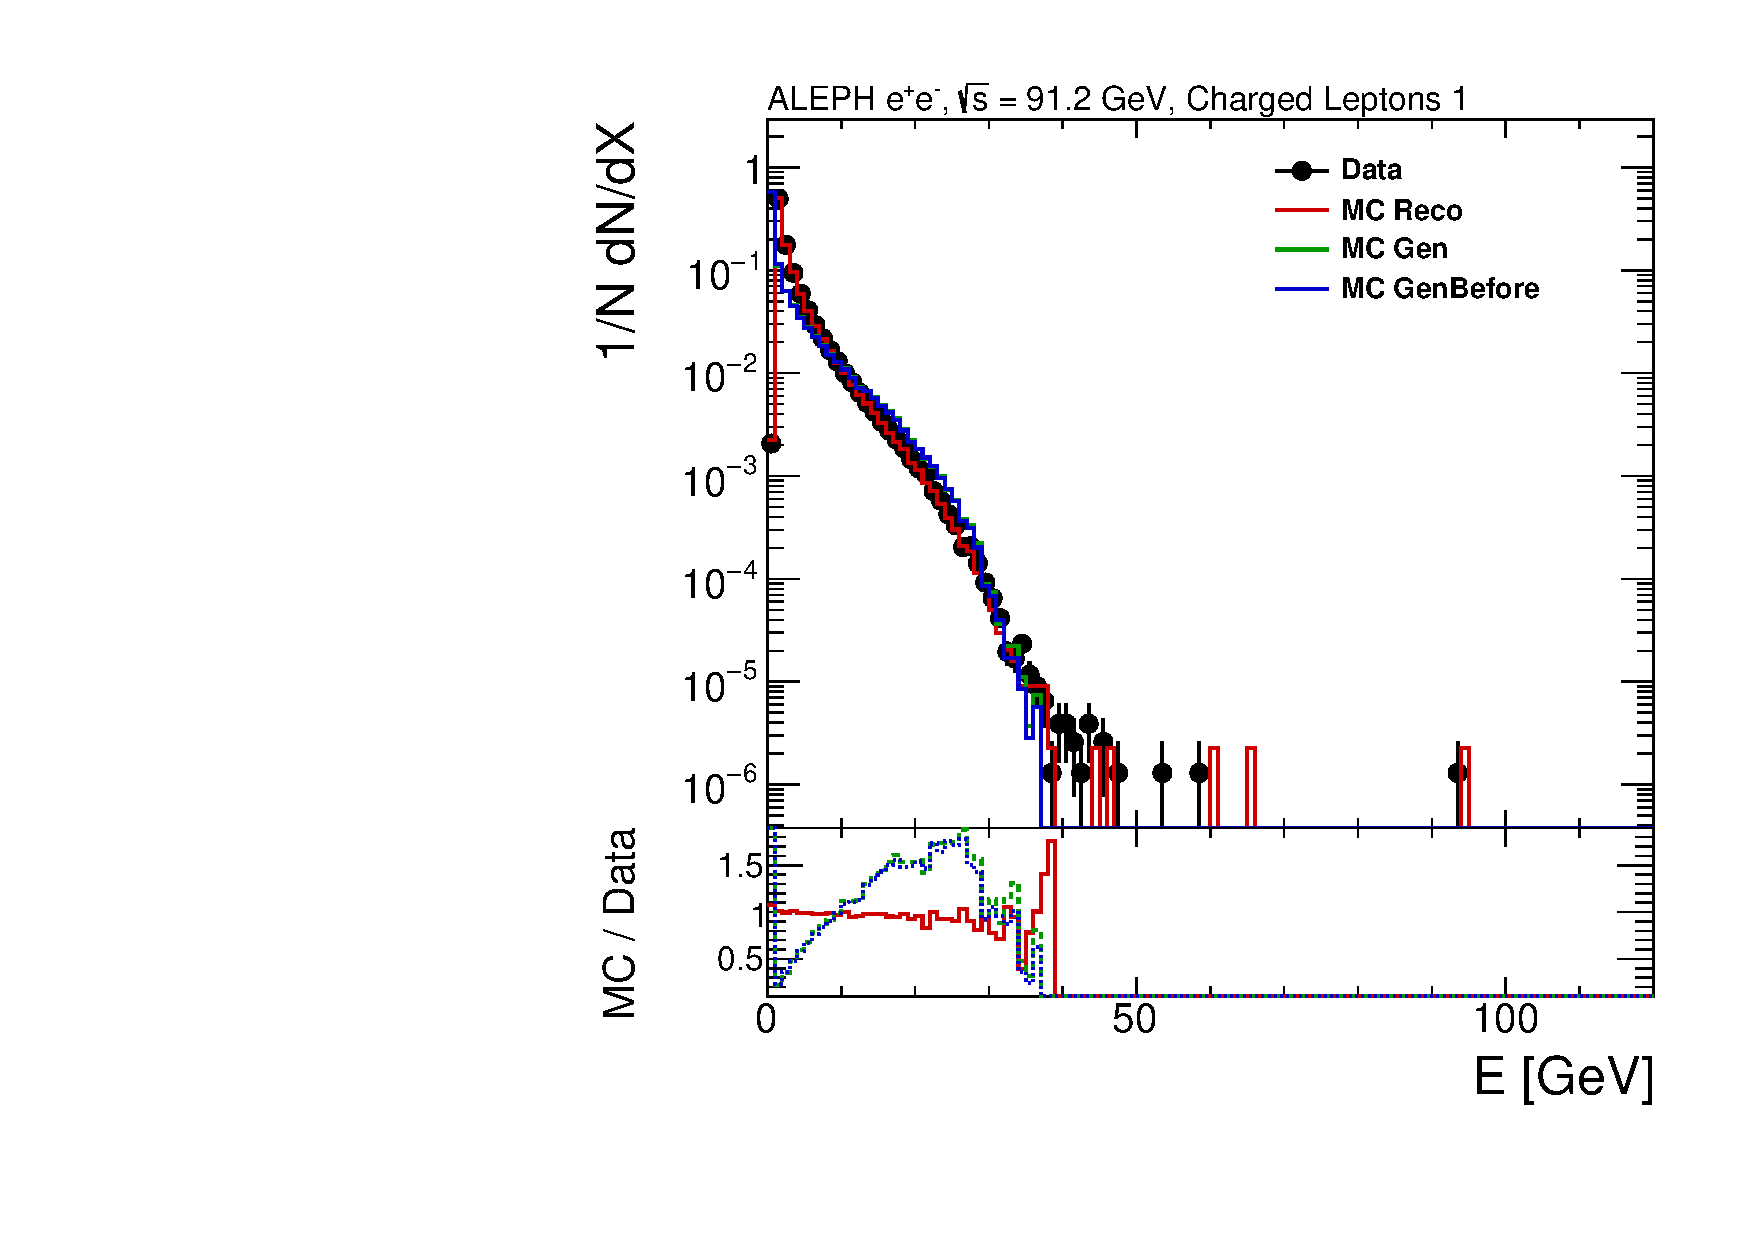
\includegraphics[width=0.325\textwidth]{../Studies/PreliminaryResult/2026-02-17_thrust_iter5/pwflag_kinematics/pwflag1_energy.pdf}
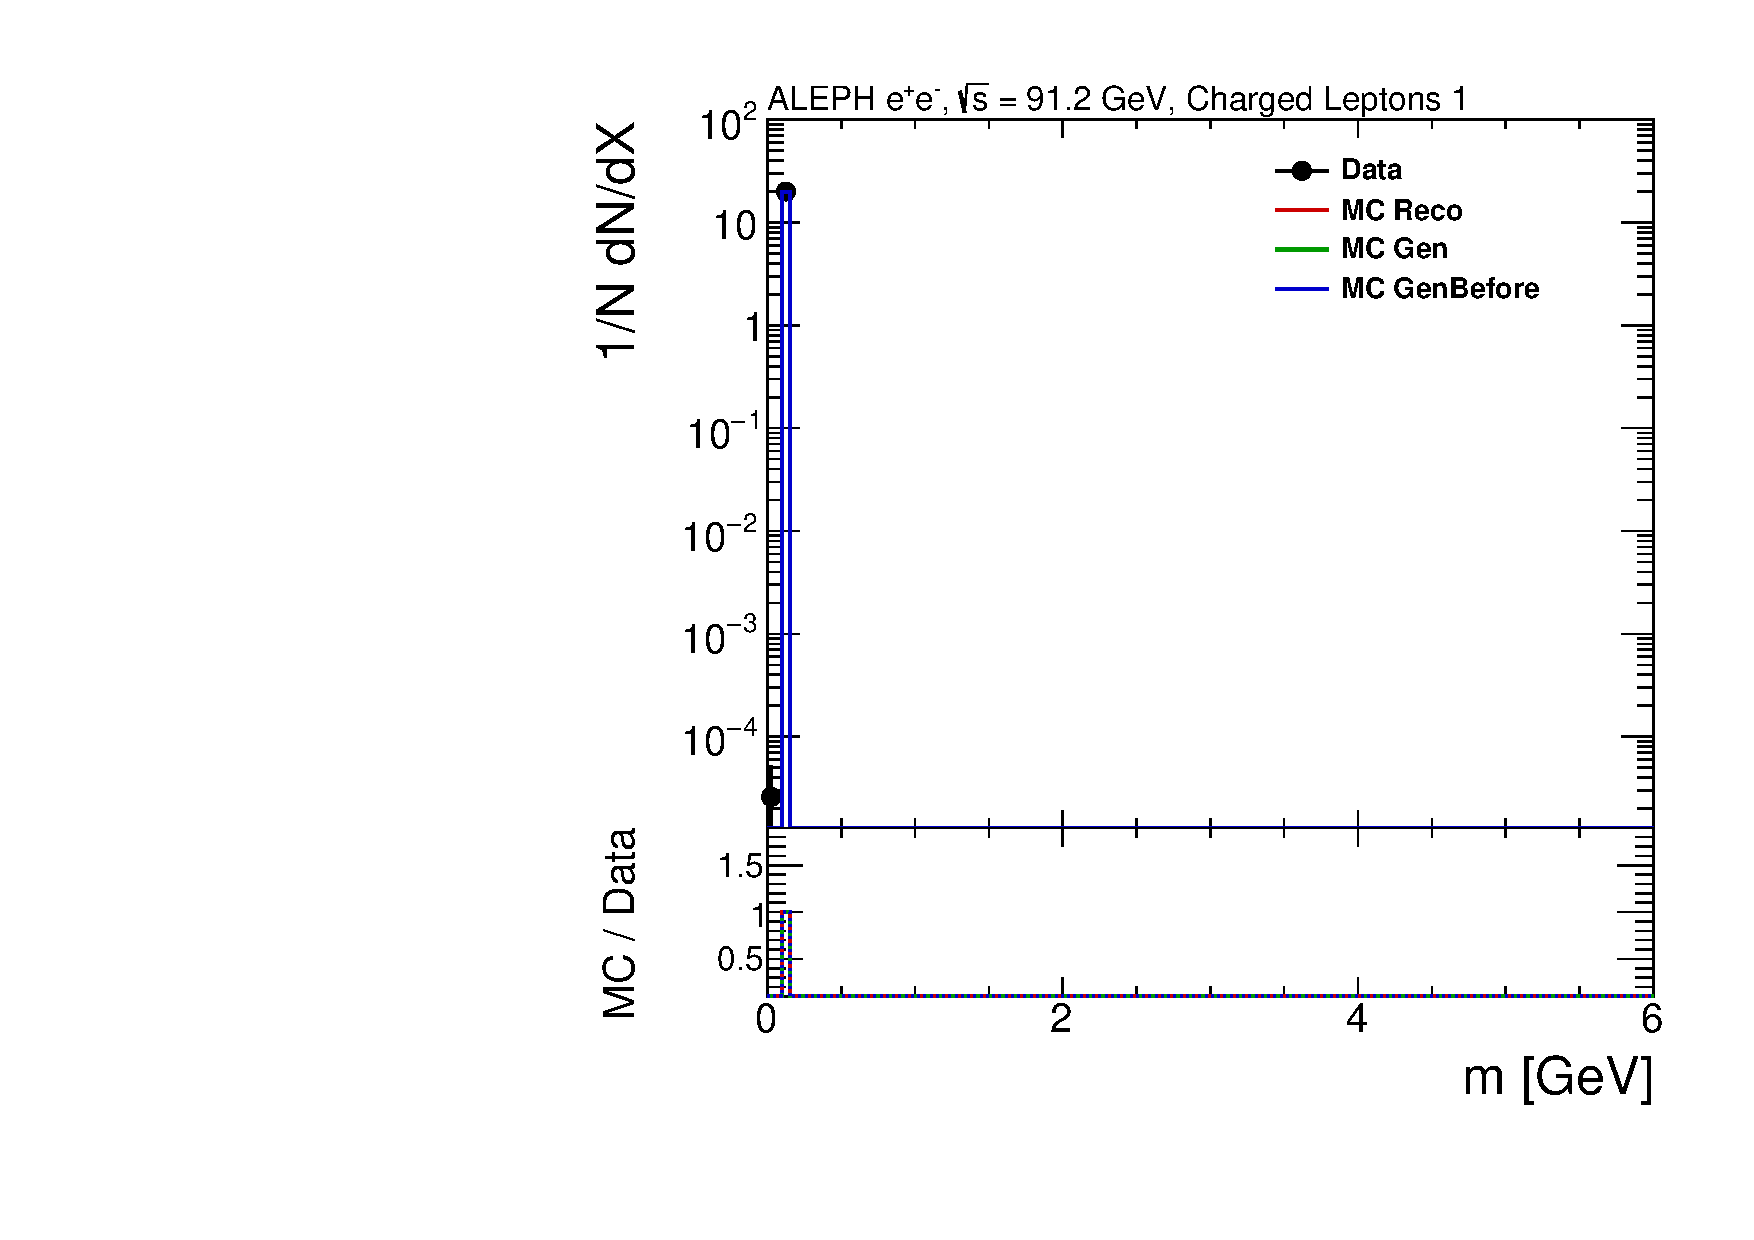
\includegraphics[width=0.325\textwidth]{../Studies/PreliminaryResult/2026-02-17_thrust_iter5/pwflag_kinematics/pwflag1_mass.pdf}
\caption{Complete \texttt{pwflag}=1 kinematic set.}
\label{fig:pwflag1_full}
\end{figure}

\noindent
Figure~\ref{fig:pwflag1_full} shows the first charged-lepton class used in the nominal object
list; these lower-rate objects still affect event axes in asymmetric topologies. Relative to
charged tracks, this category has smaller yields and larger statistical fluctuations, but the
detector-level and MC shapes remain consistent across the main selection observables. The
comparison is important because isolated energetic leptons can rotate the thrust axis in otherwise
two-jet-like events and can therefore influence migration in specific bins.

\begin{figure}[t!]
\centering
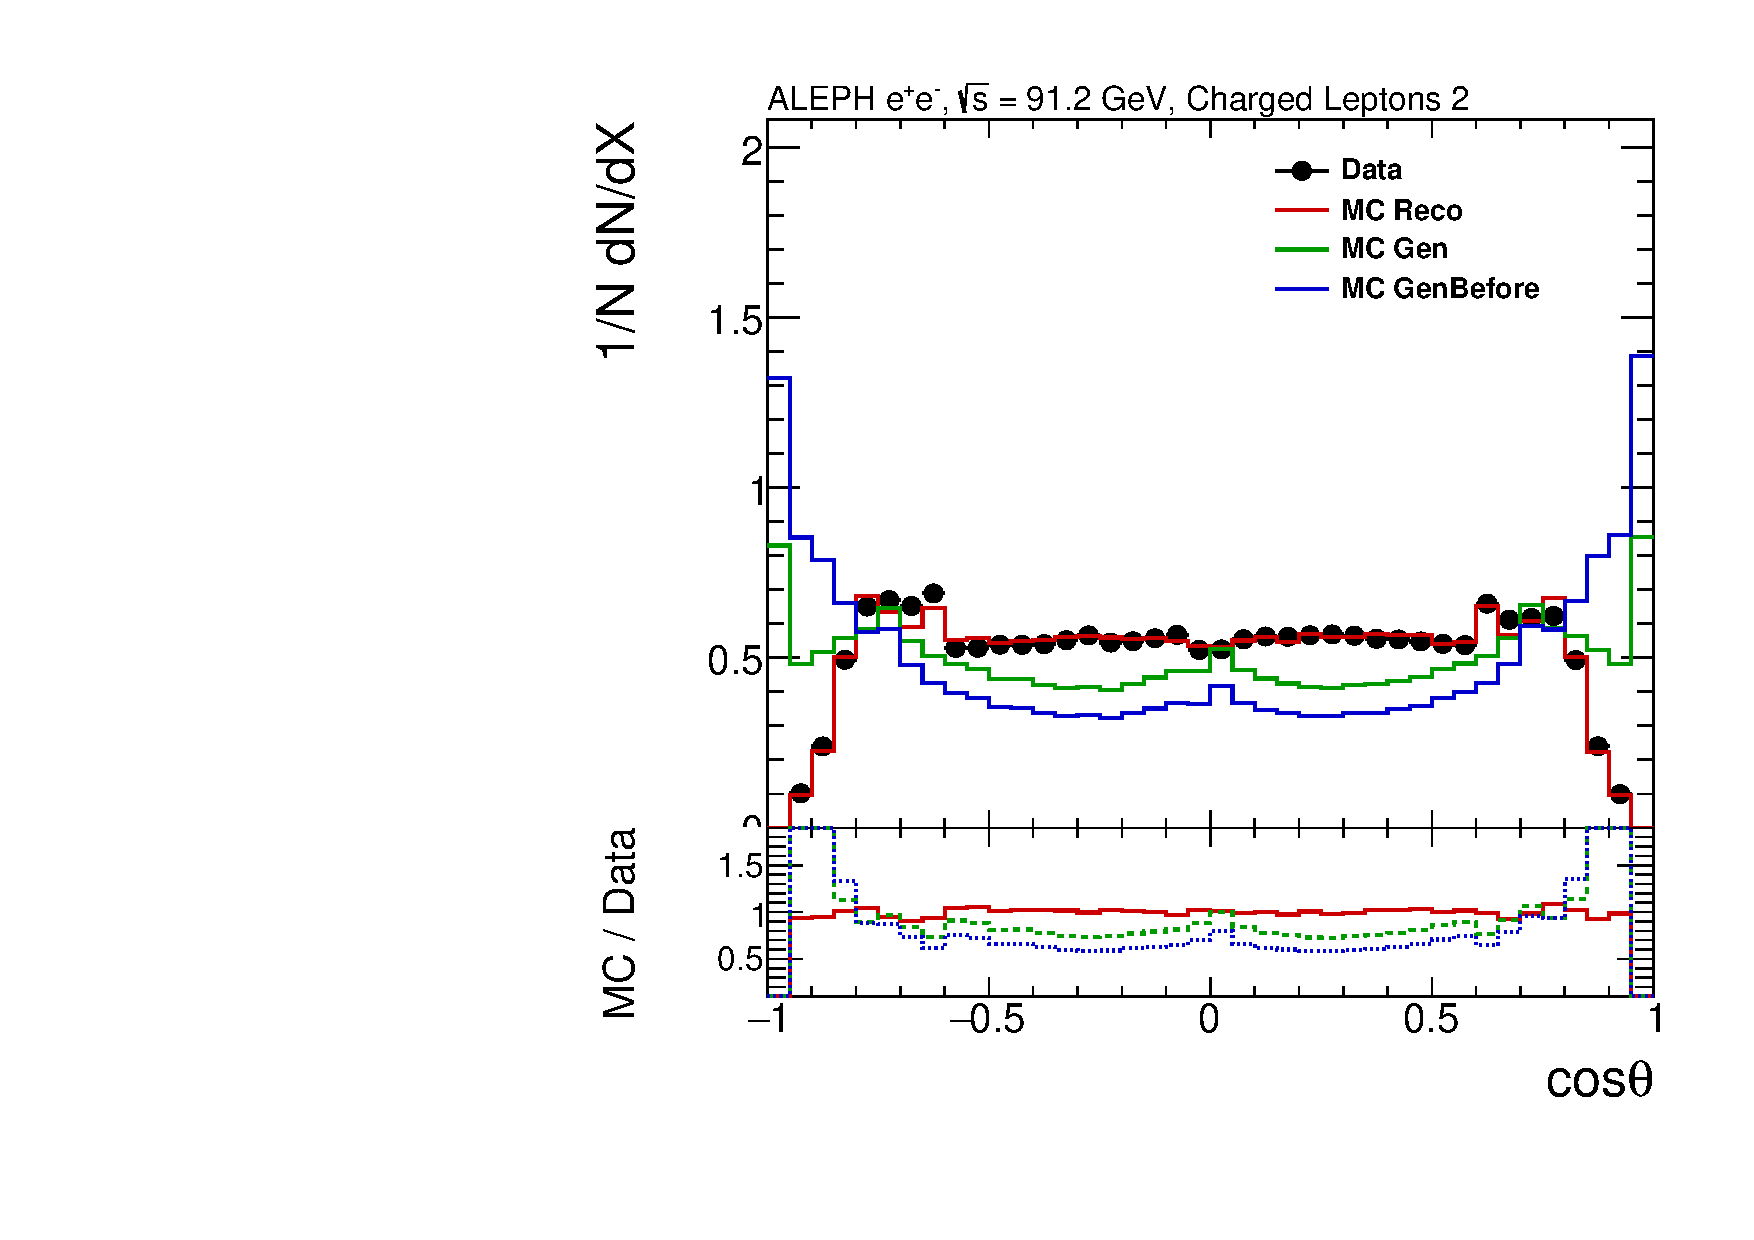
\includegraphics[width=0.325\textwidth]{../Studies/PreliminaryResult/2026-02-17_thrust_iter5/pwflag_kinematics/pwflag2_cosTheta.pdf}
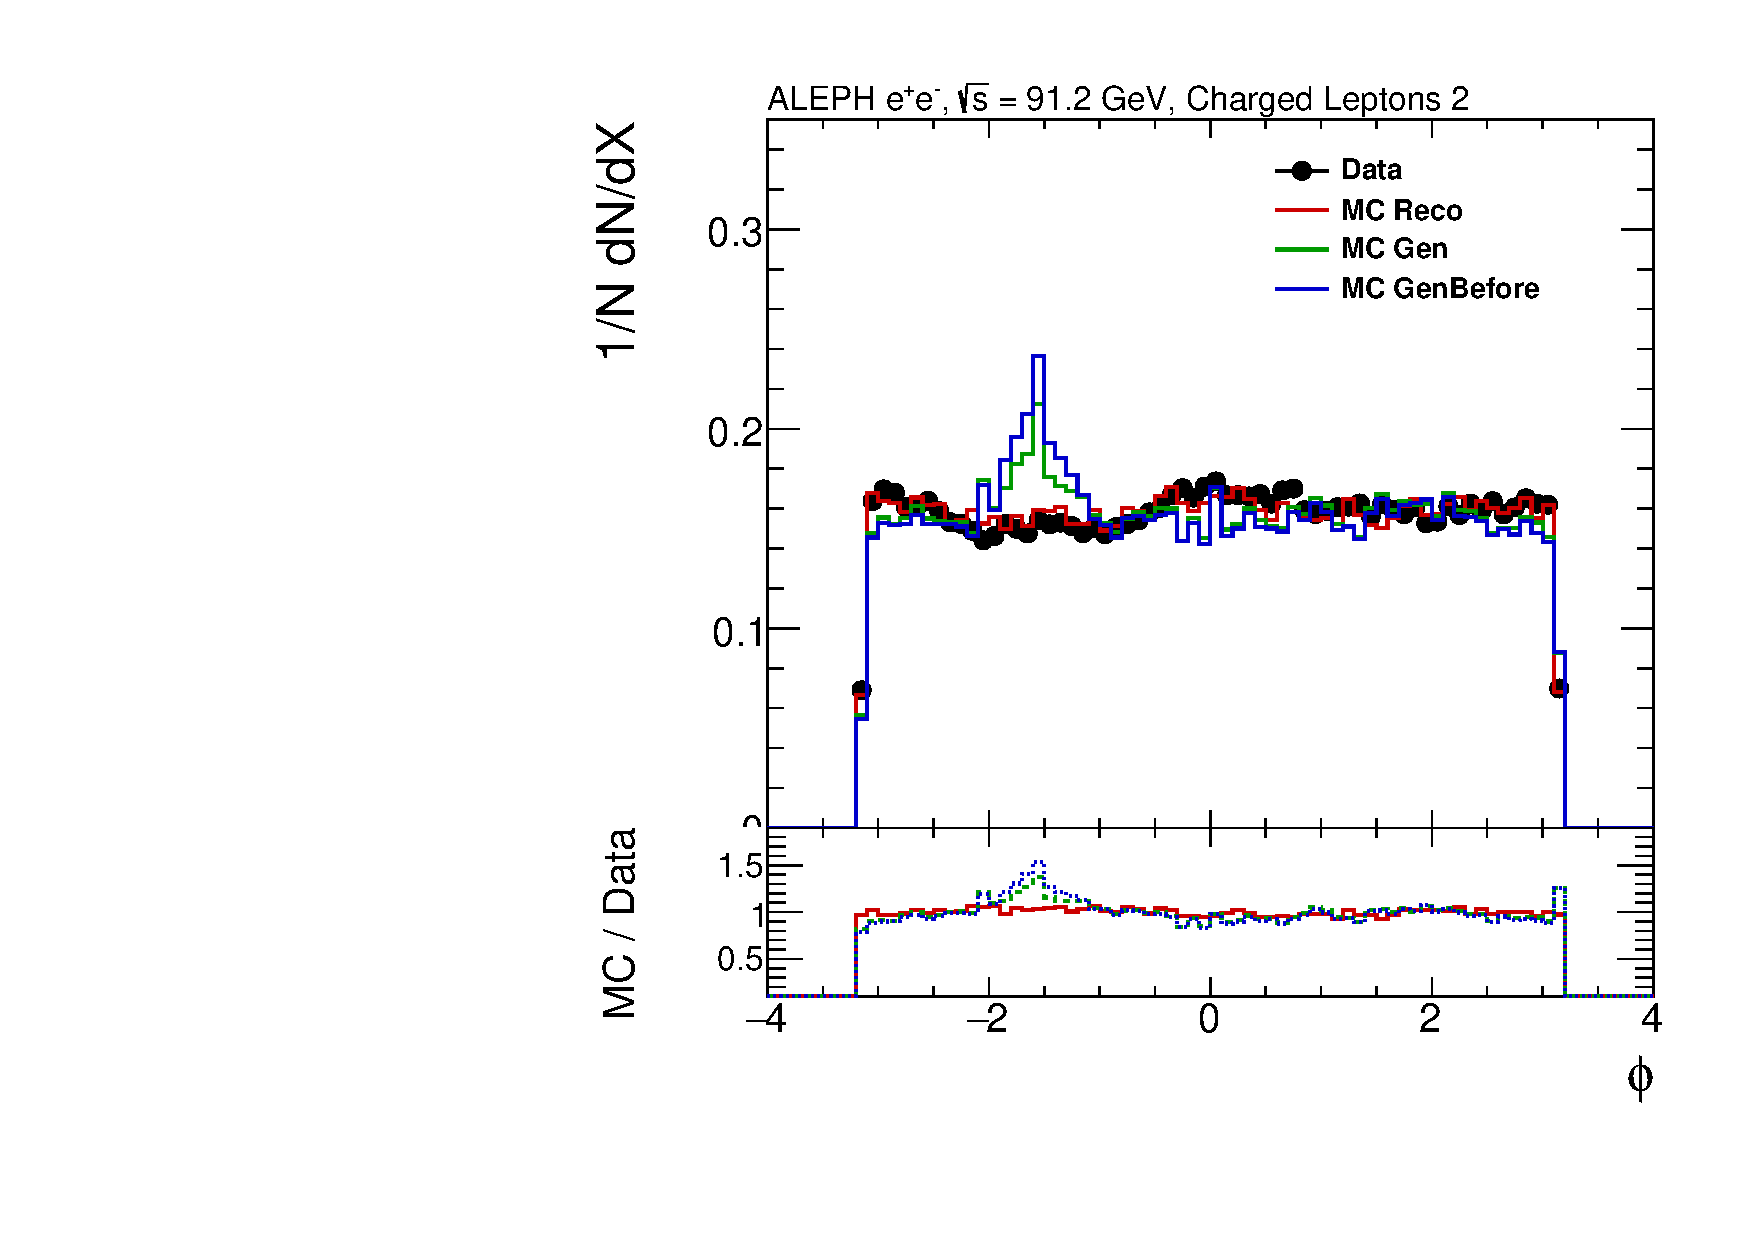
\includegraphics[width=0.325\textwidth]{../Studies/PreliminaryResult/2026-02-17_thrust_iter5/pwflag_kinematics/pwflag2_phi.pdf}
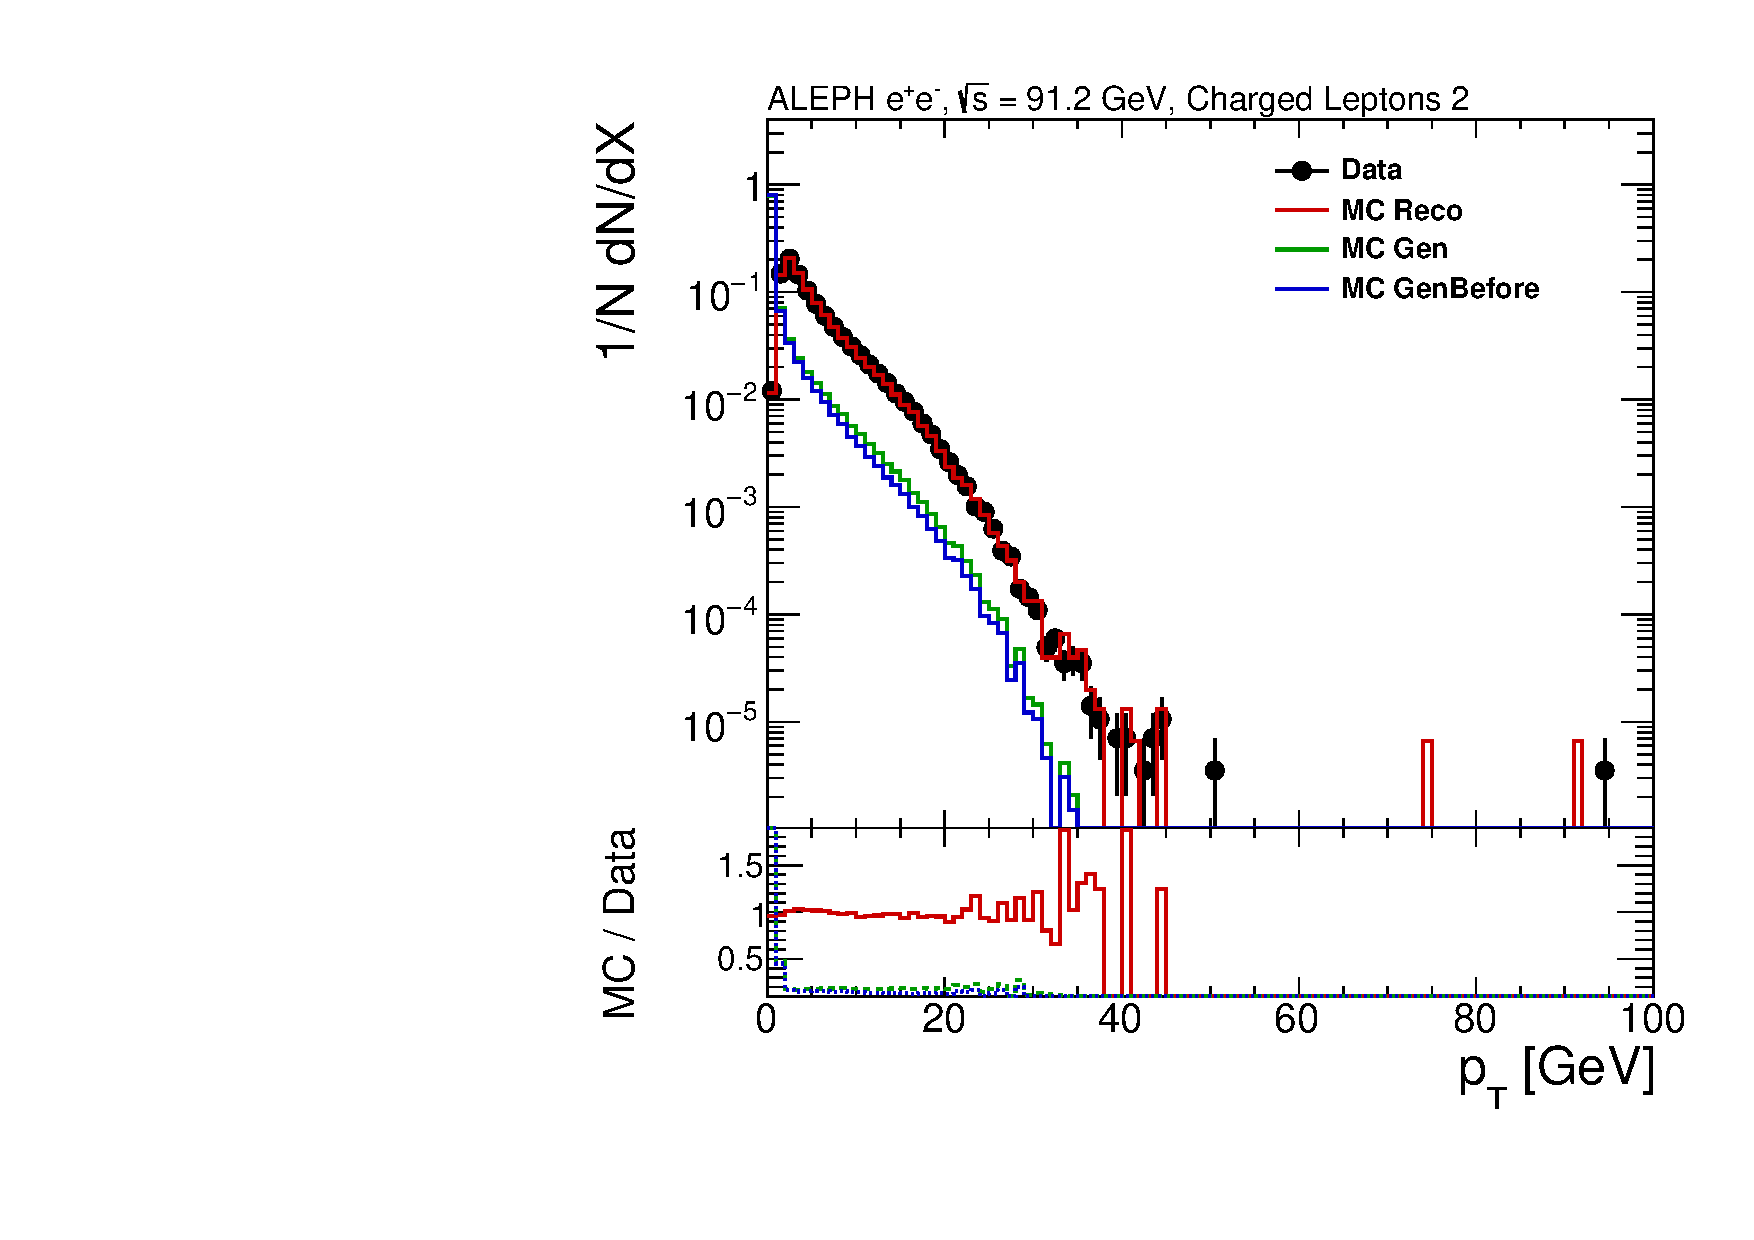
\includegraphics[width=0.325\textwidth]{../Studies/PreliminaryResult/2026-02-17_thrust_iter5/pwflag_kinematics/pwflag2_pt.pdf}
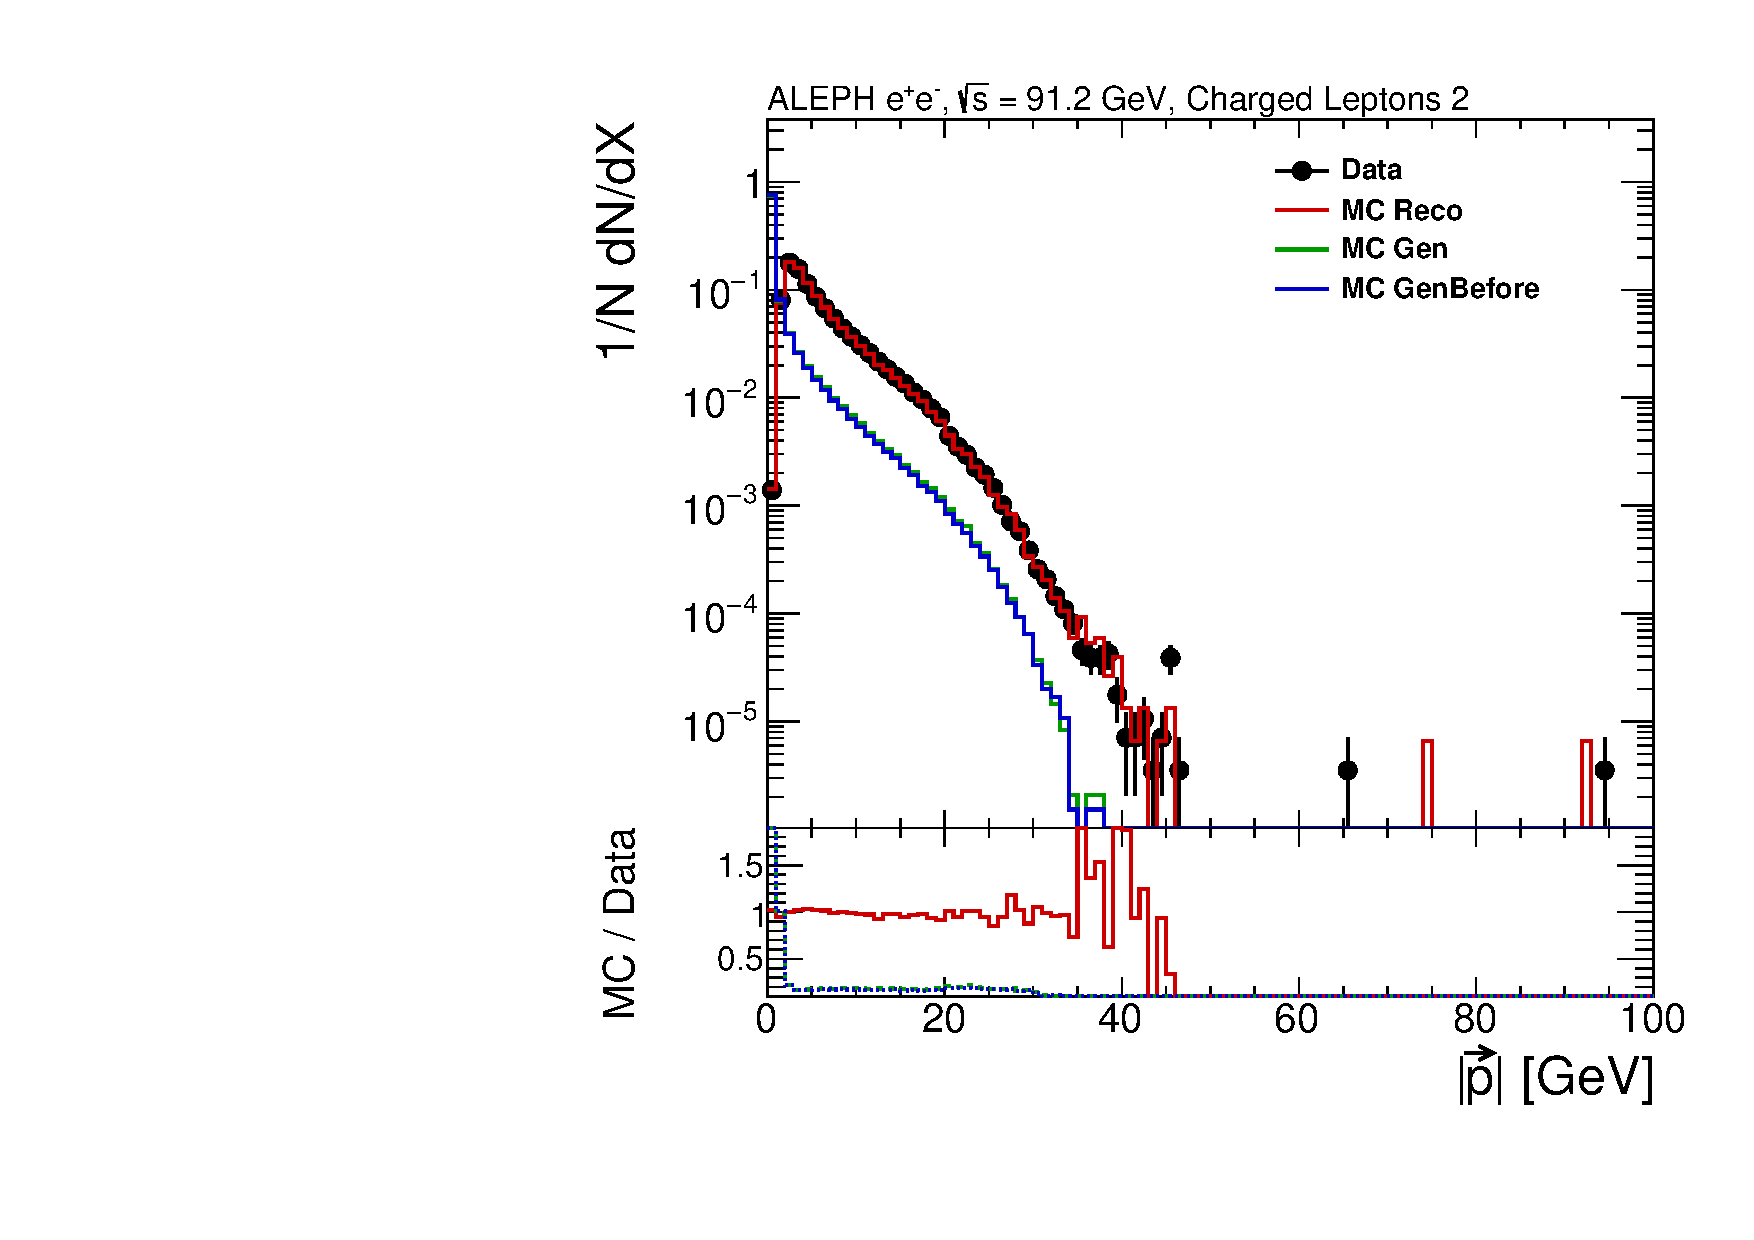
\includegraphics[width=0.325\textwidth]{../Studies/PreliminaryResult/2026-02-17_thrust_iter5/pwflag_kinematics/pwflag2_pmag.pdf}
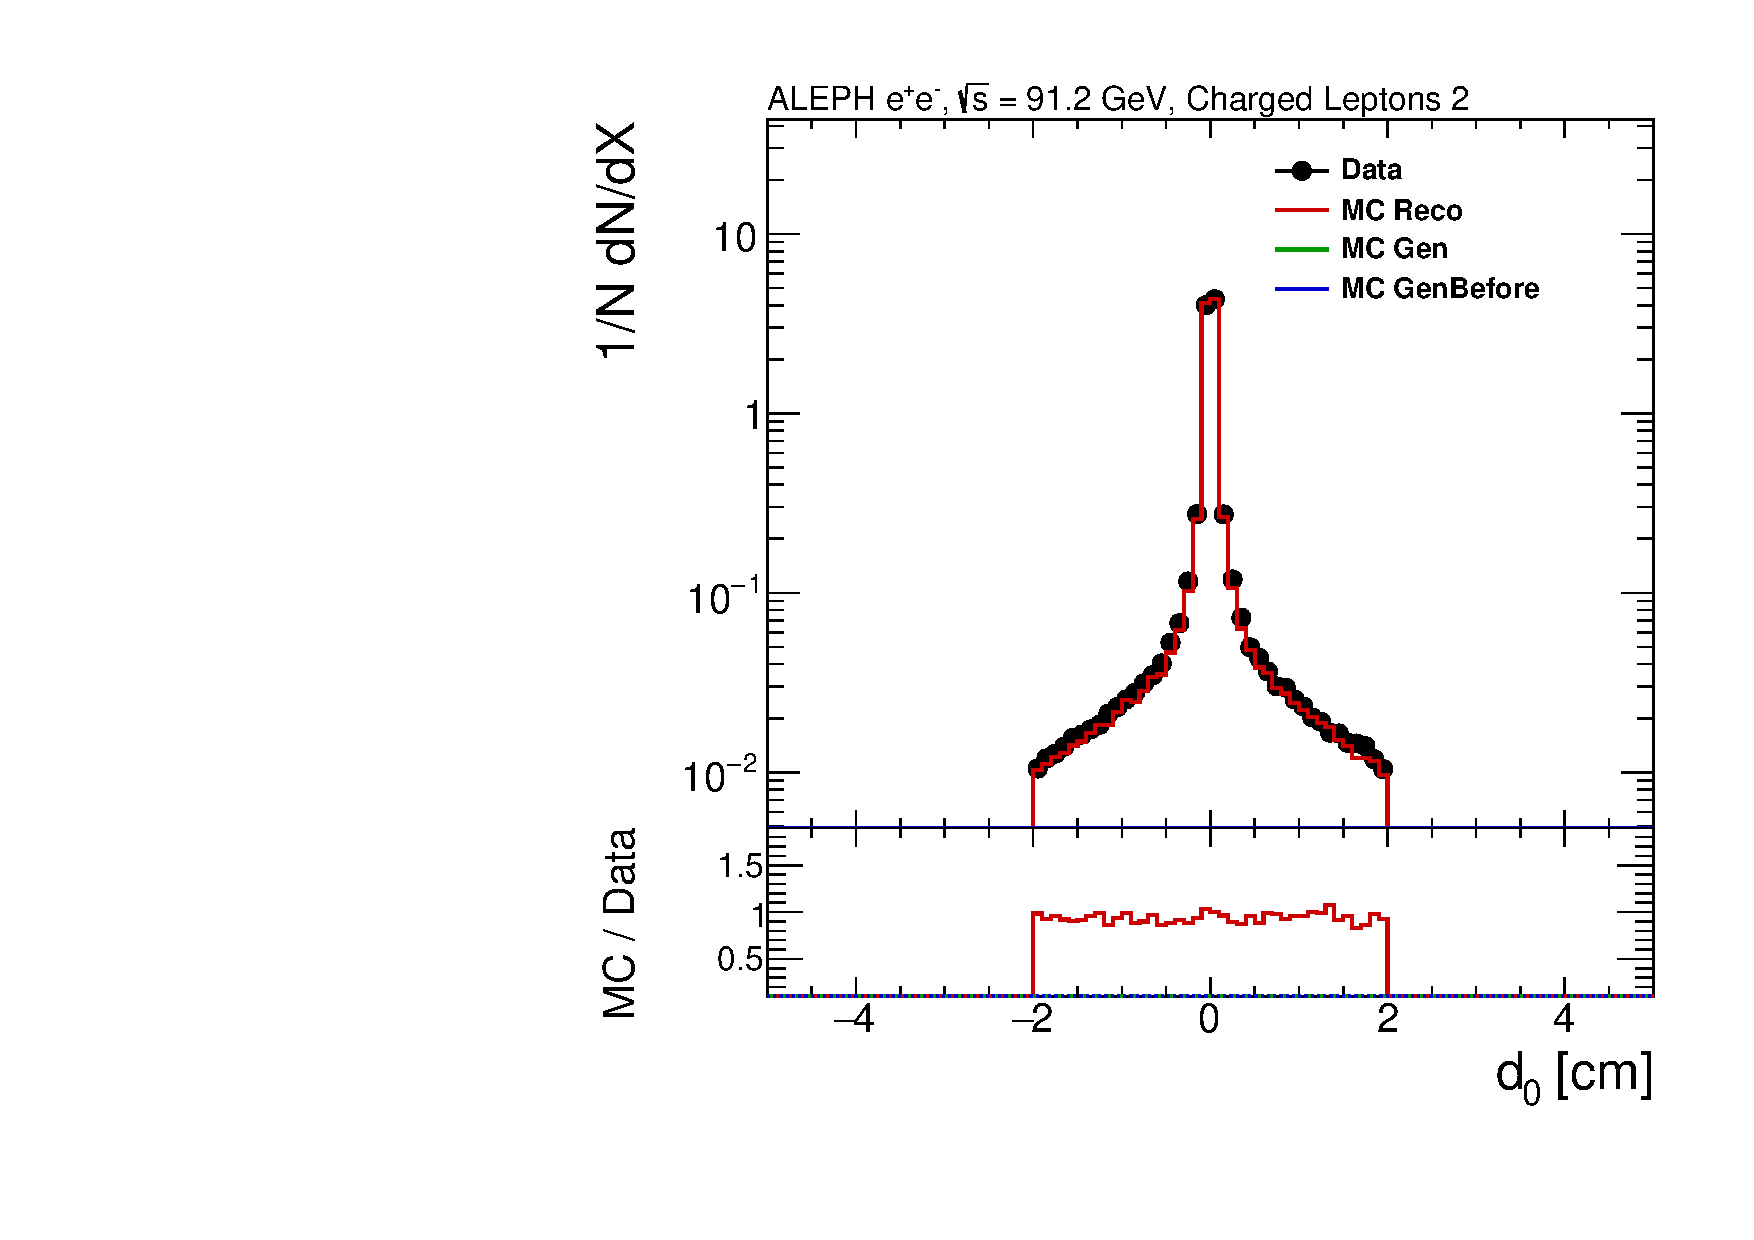
\includegraphics[width=0.325\textwidth]{../Studies/PreliminaryResult/2026-02-17_thrust_iter5/pwflag_kinematics/pwflag2_d0.pdf}
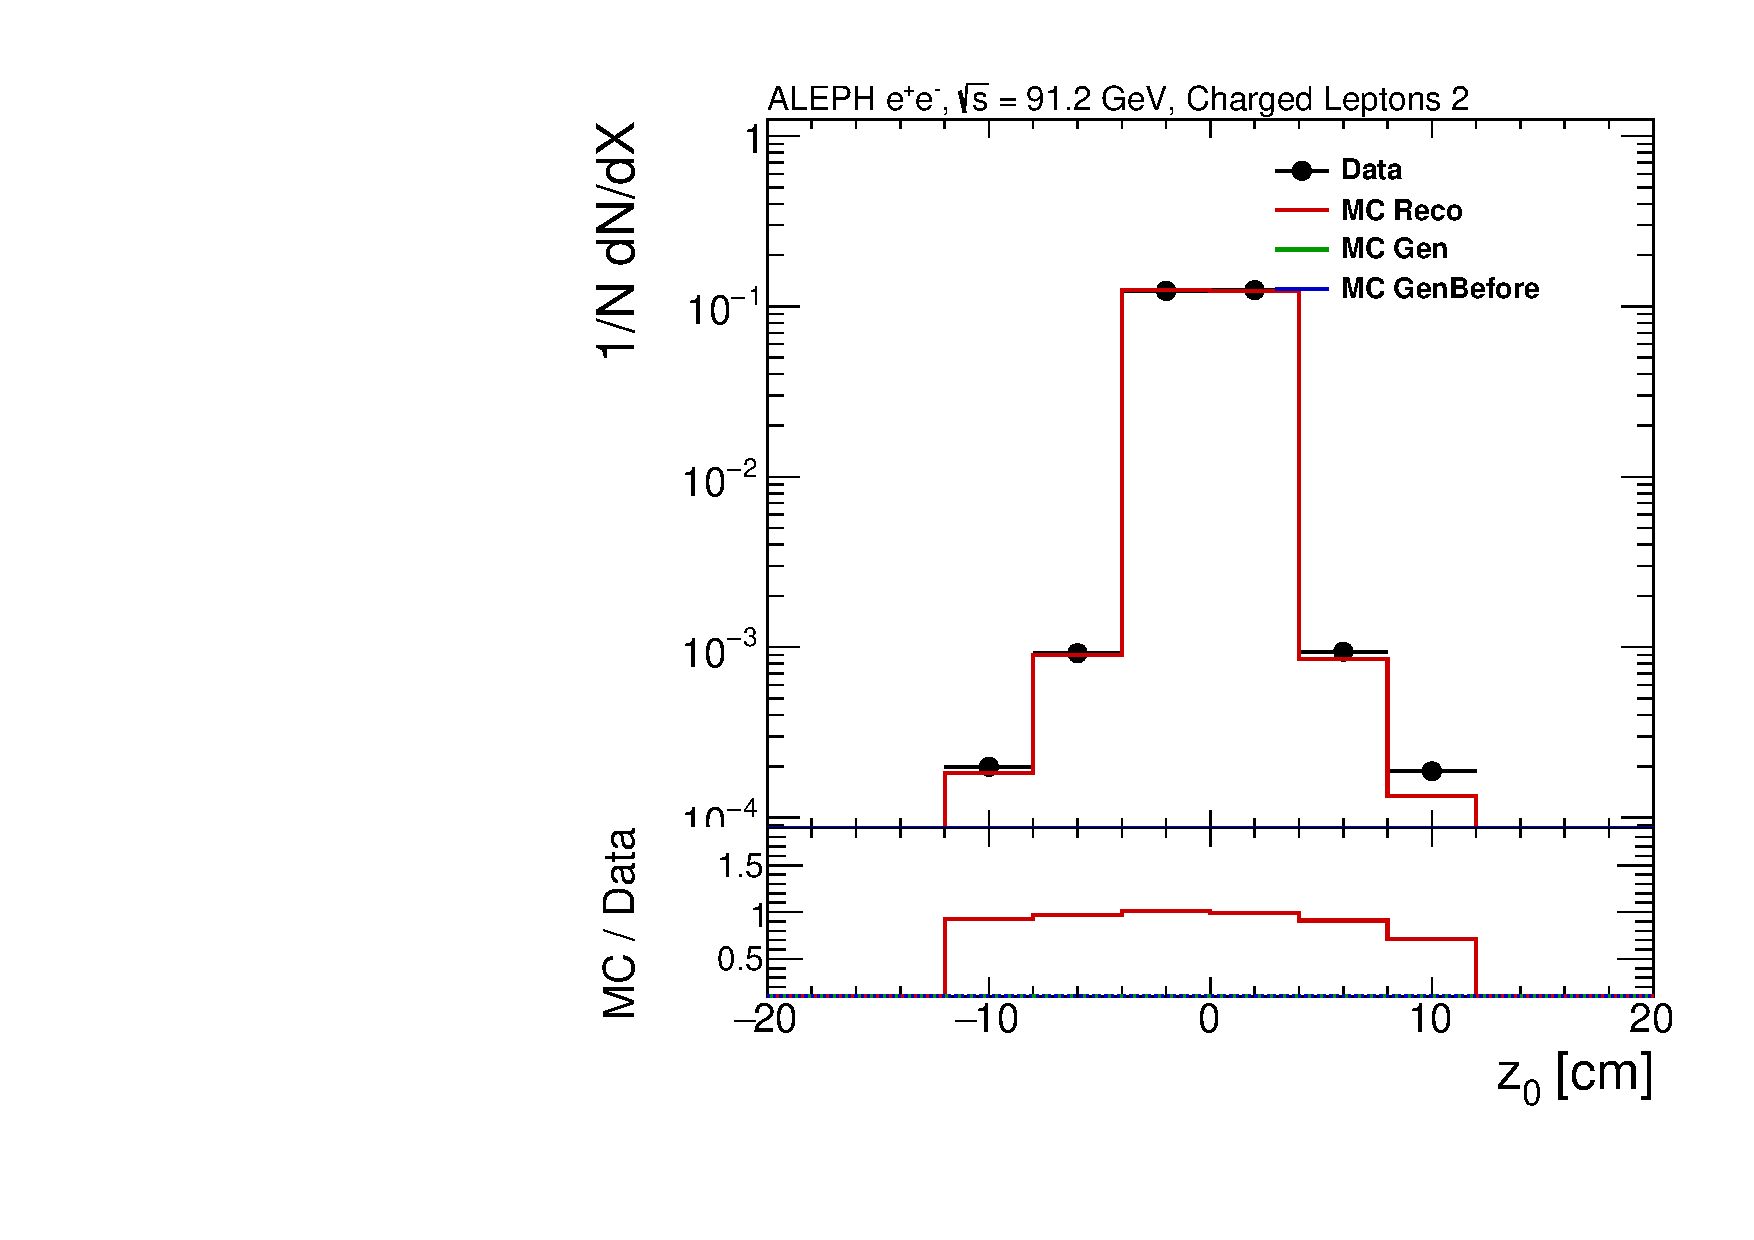
\includegraphics[width=0.325\textwidth]{../Studies/PreliminaryResult/2026-02-17_thrust_iter5/pwflag_kinematics/pwflag2_z0.pdf}
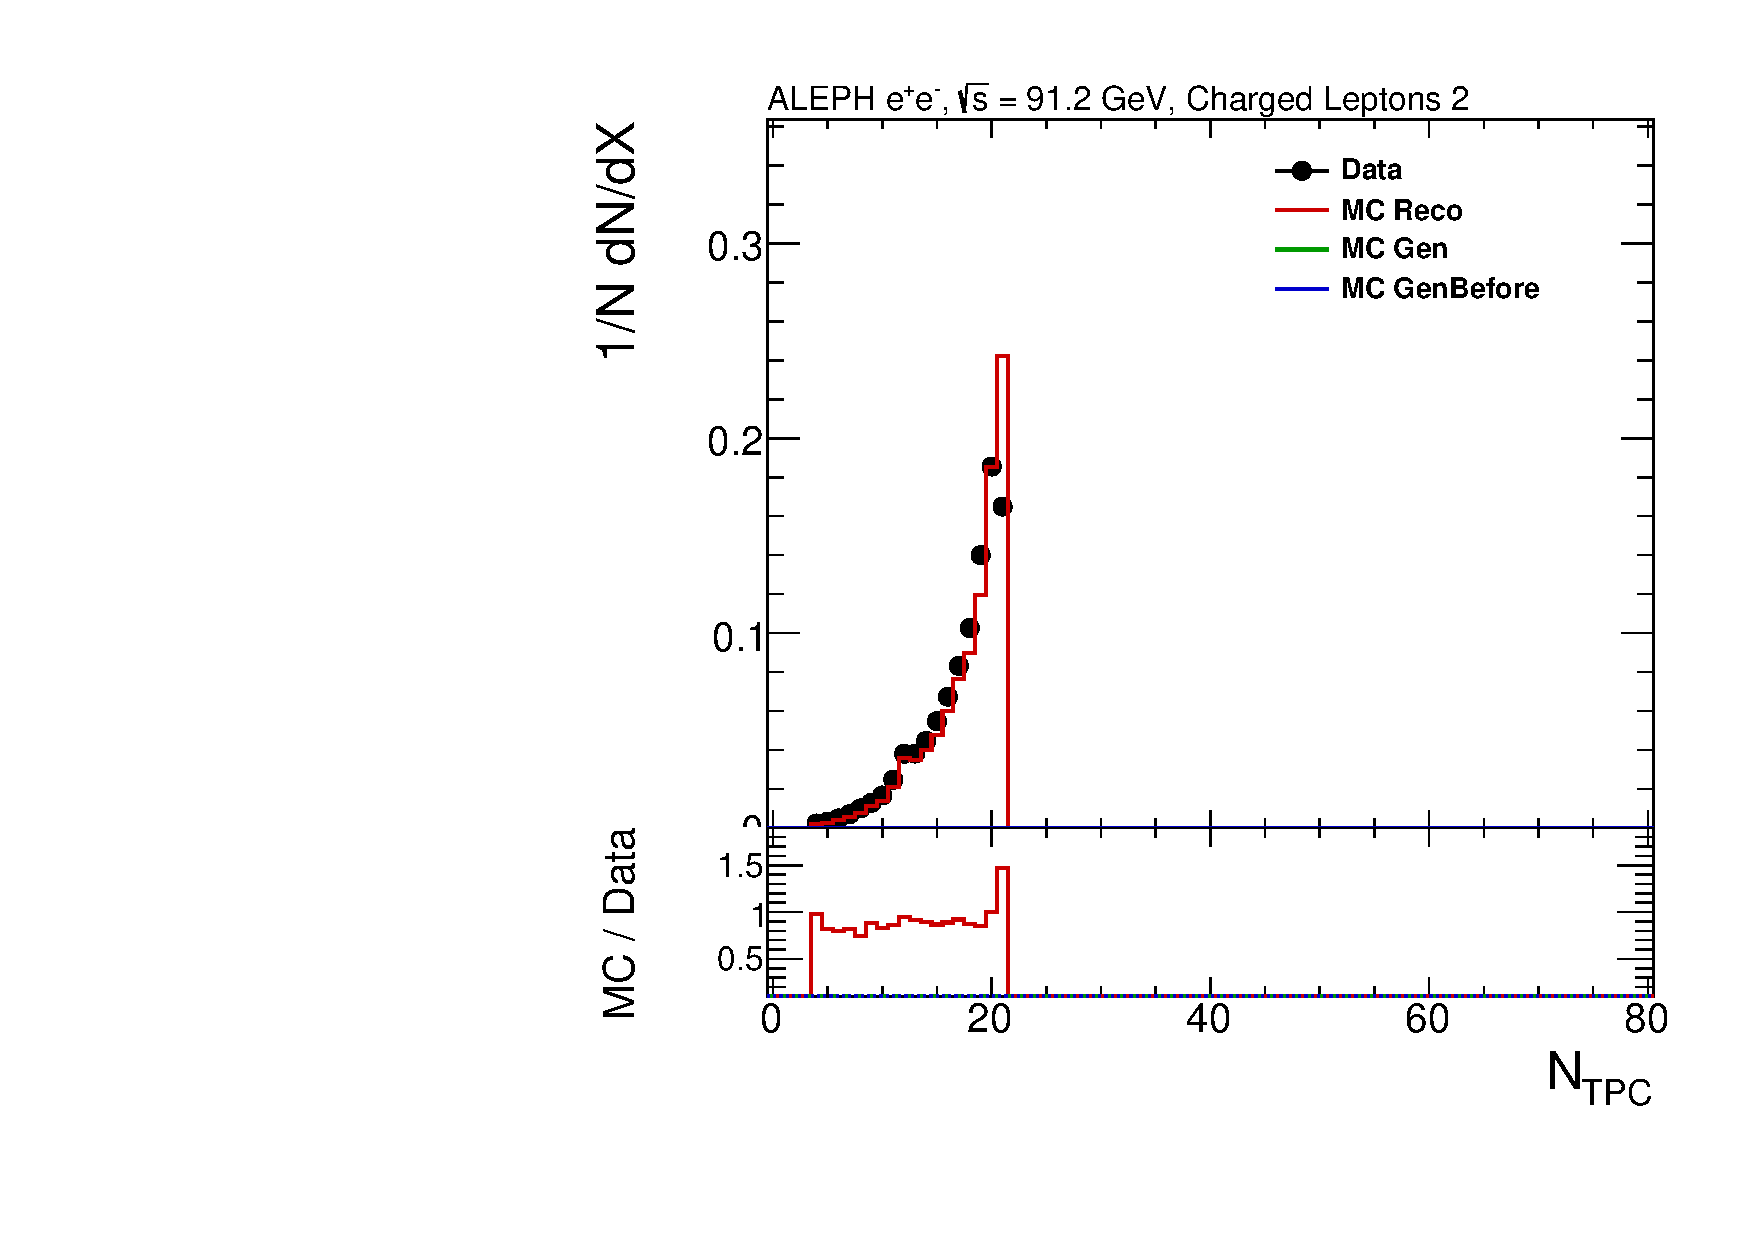
\includegraphics[width=0.325\textwidth]{../Studies/PreliminaryResult/2026-02-17_thrust_iter5/pwflag_kinematics/pwflag2_ntpc.pdf}
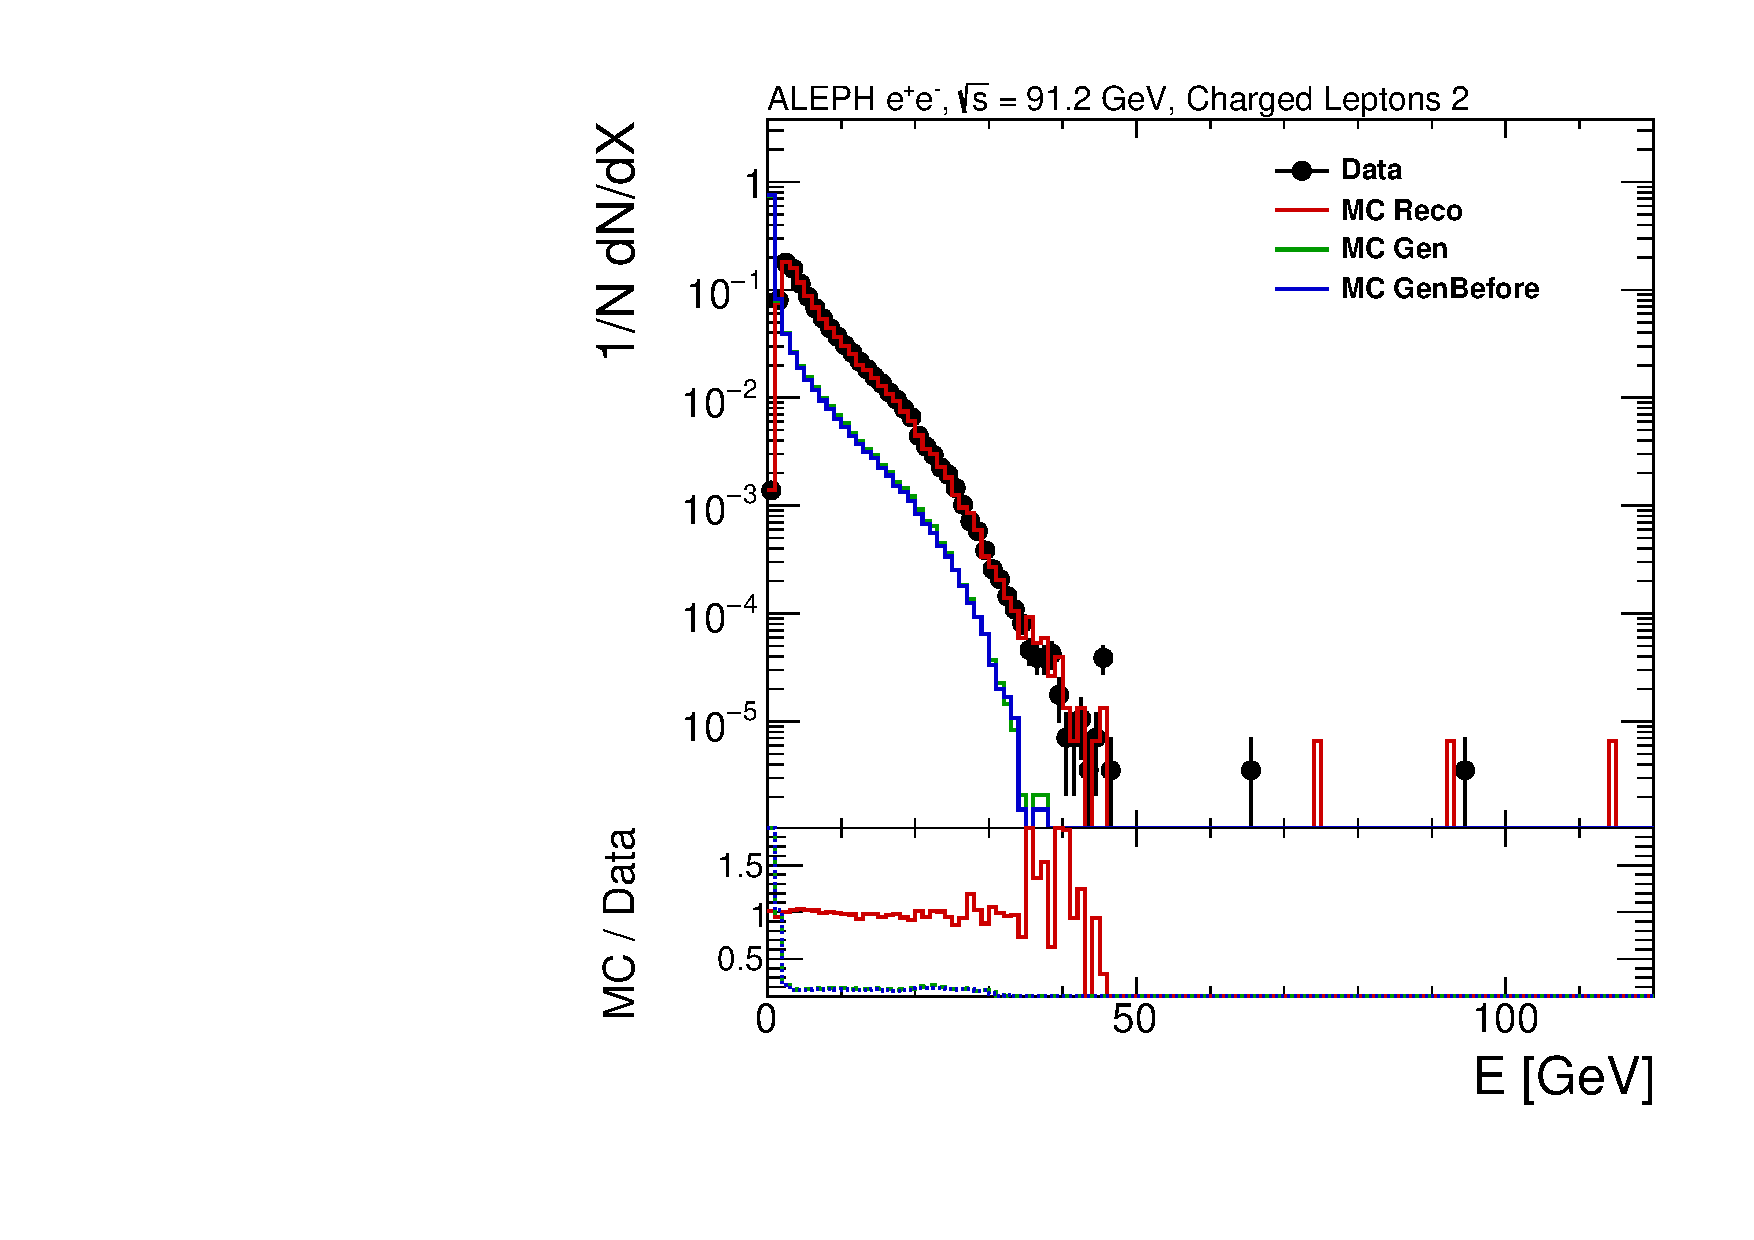
\includegraphics[width=0.325\textwidth]{../Studies/PreliminaryResult/2026-02-17_thrust_iter5/pwflag_kinematics/pwflag2_energy.pdf}
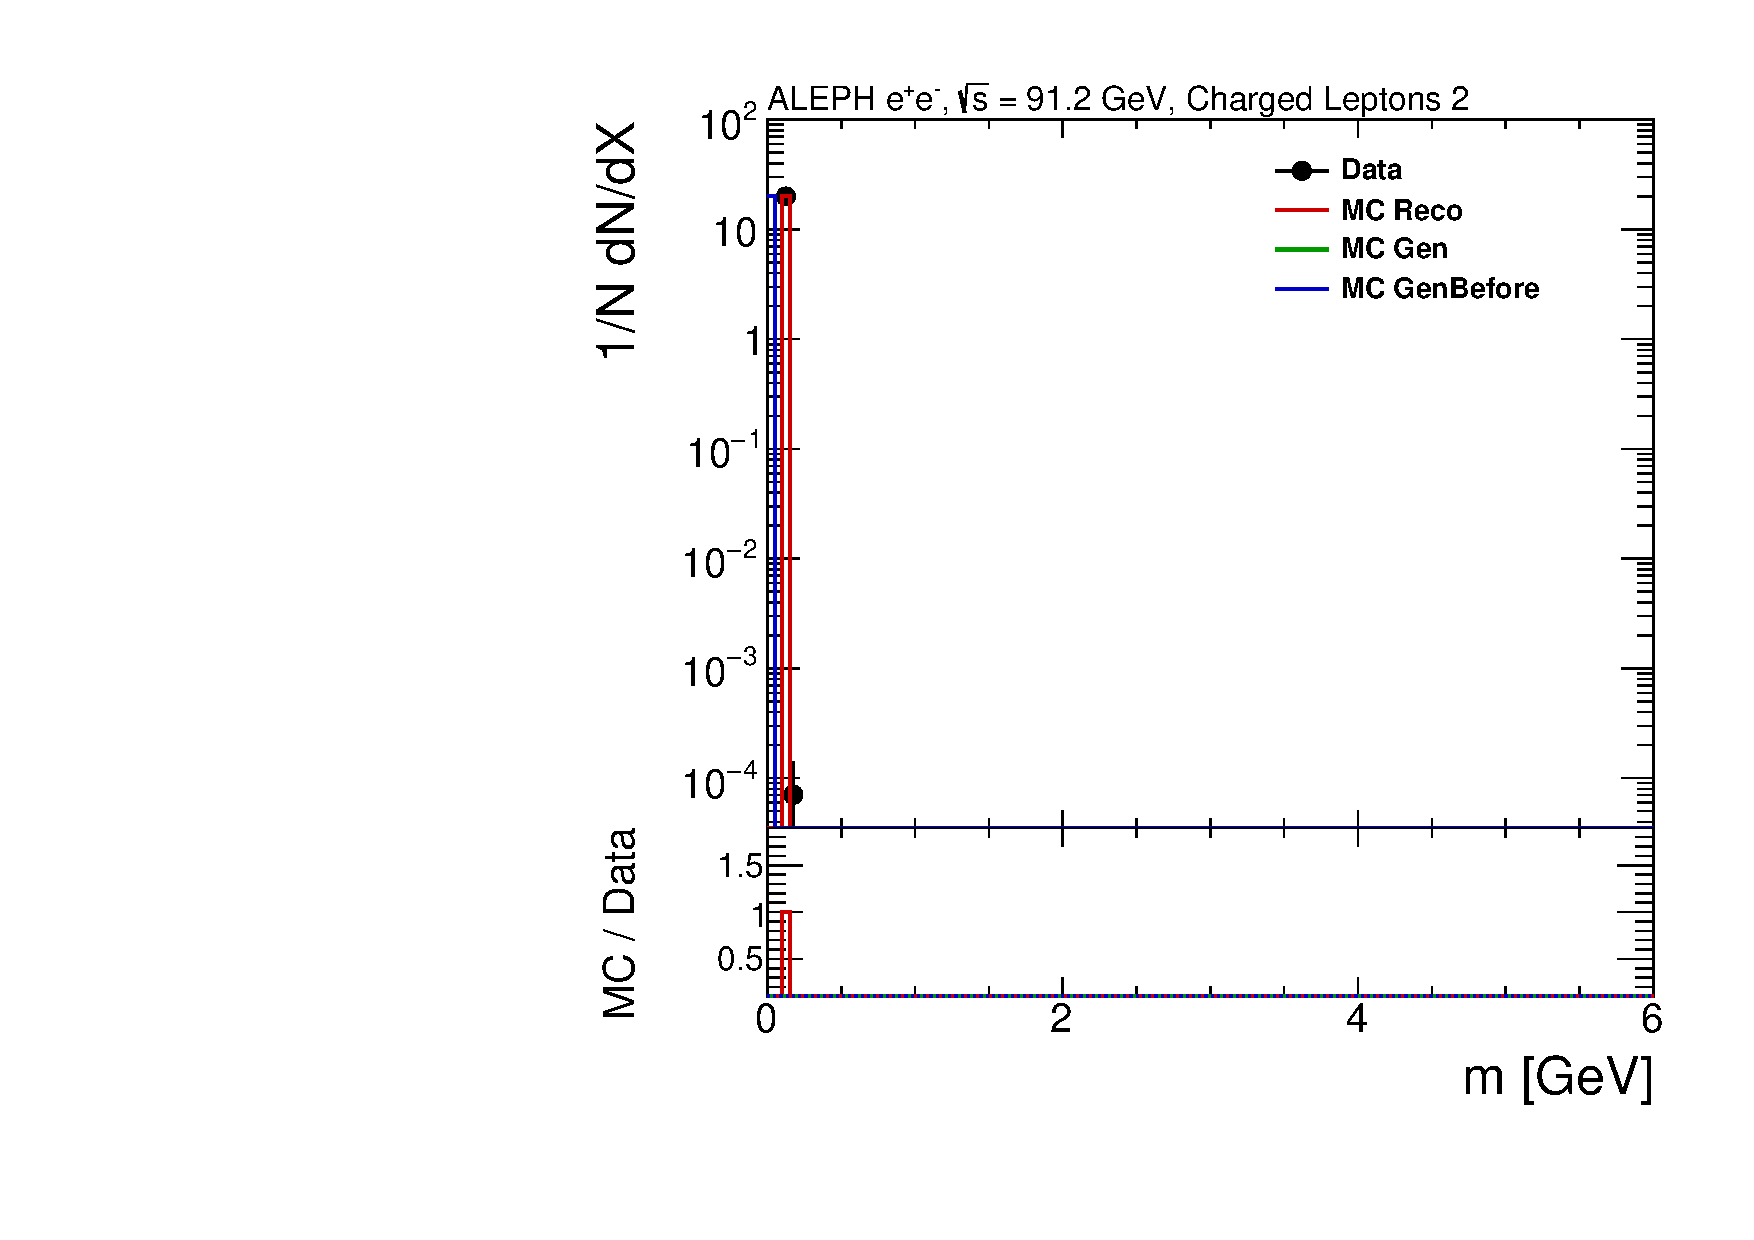
\includegraphics[width=0.325\textwidth]{../Studies/PreliminaryResult/2026-02-17_thrust_iter5/pwflag_kinematics/pwflag2_mass.pdf}
\caption{Complete \texttt{pwflag}=2 kinematic set.}
\label{fig:pwflag2_full}
\end{figure}

\noindent
Figure~\ref{fig:pwflag2_full} presents the second charged-lepton category, providing a direct
cross-check of category-dependent acceptance and momentum-shape modeling. This category probes
objects with different subdetector signatures than Fig.~\ref{fig:pwflag1_full}, so agreement
here confirms that lepton-category partitioning does not induce a hidden detector asymmetry in
the thrust inputs. The high-$p_T$ and high-energy tails are monitored explicitly because even a
small mismodeling there can project onto endpoint thrust bins.

\begin{figure}[t!]
\centering
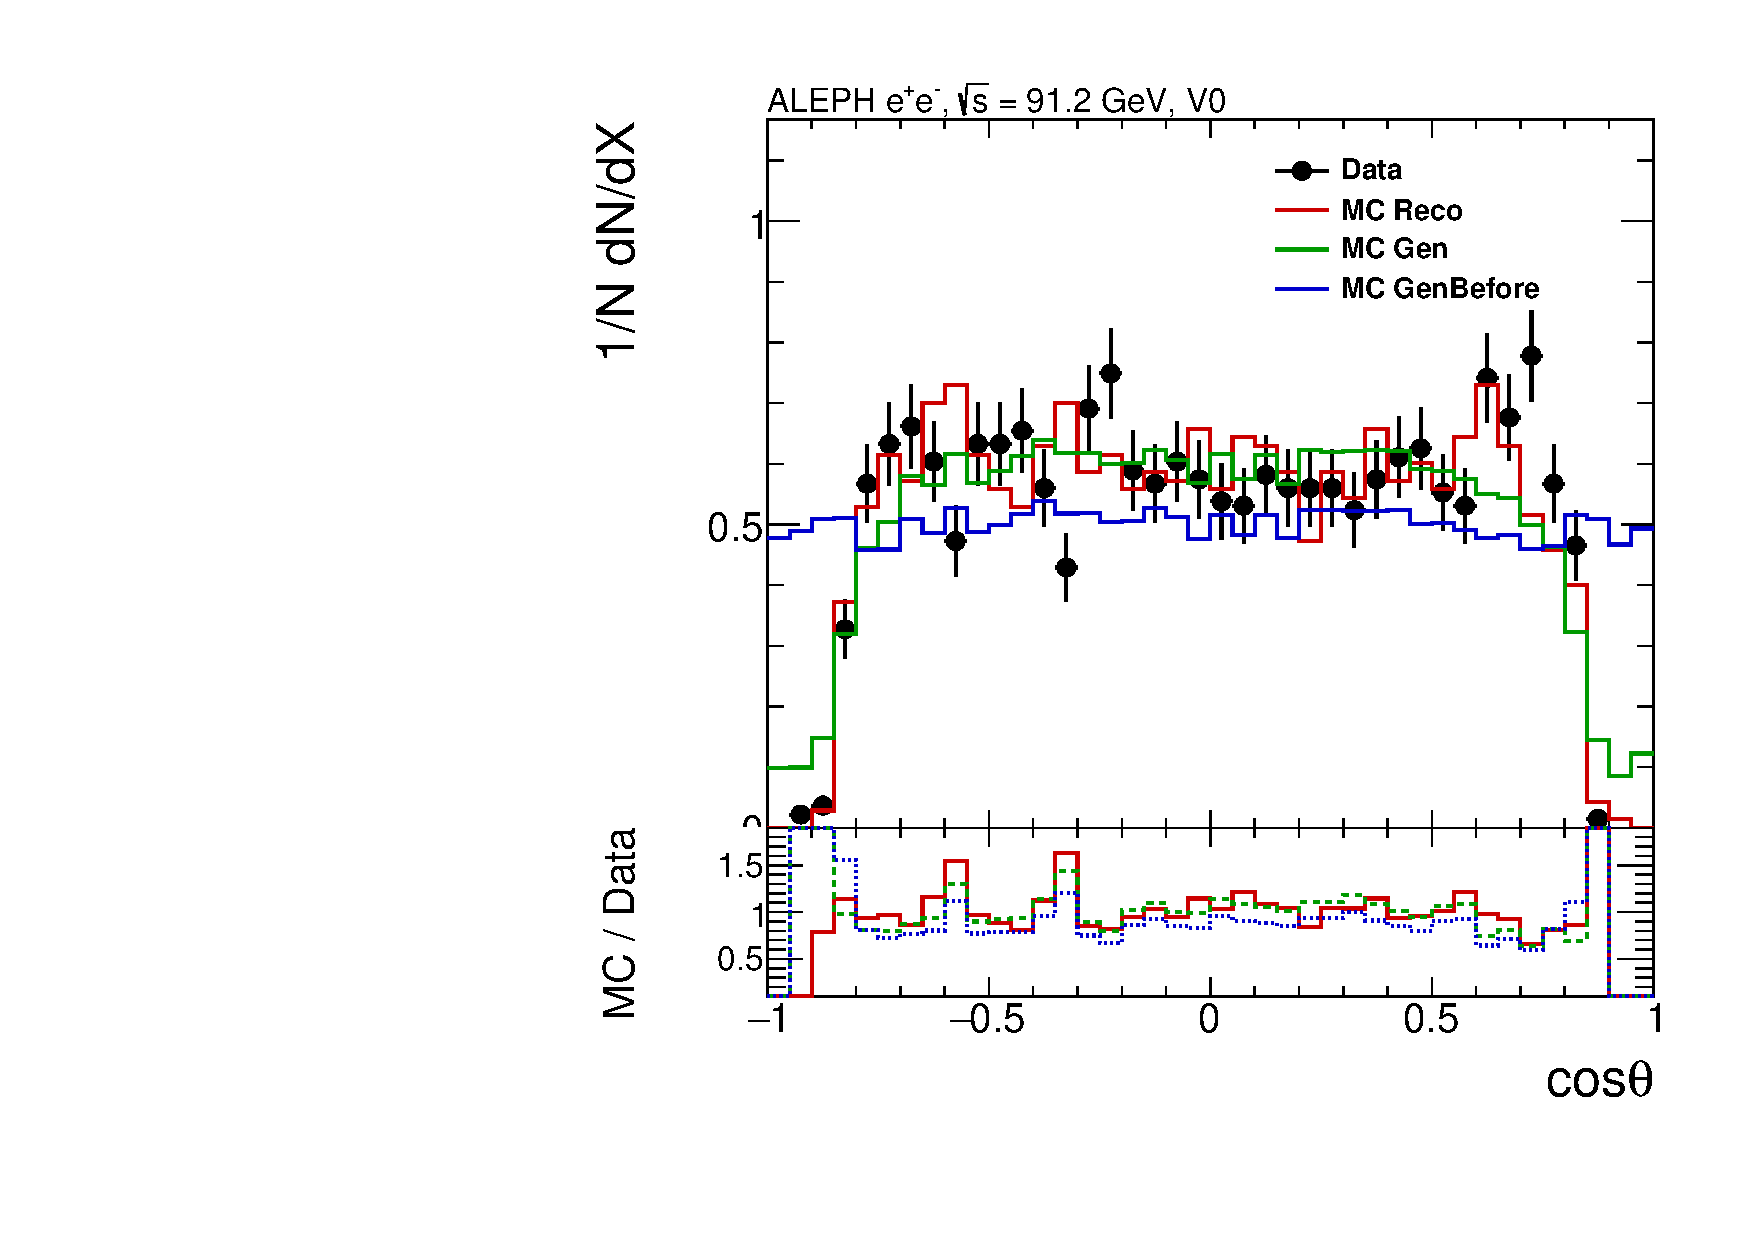
\includegraphics[width=0.325\textwidth]{../Studies/PreliminaryResult/2026-02-17_thrust_iter5/pwflag_kinematics/pwflag3_cosTheta.pdf}
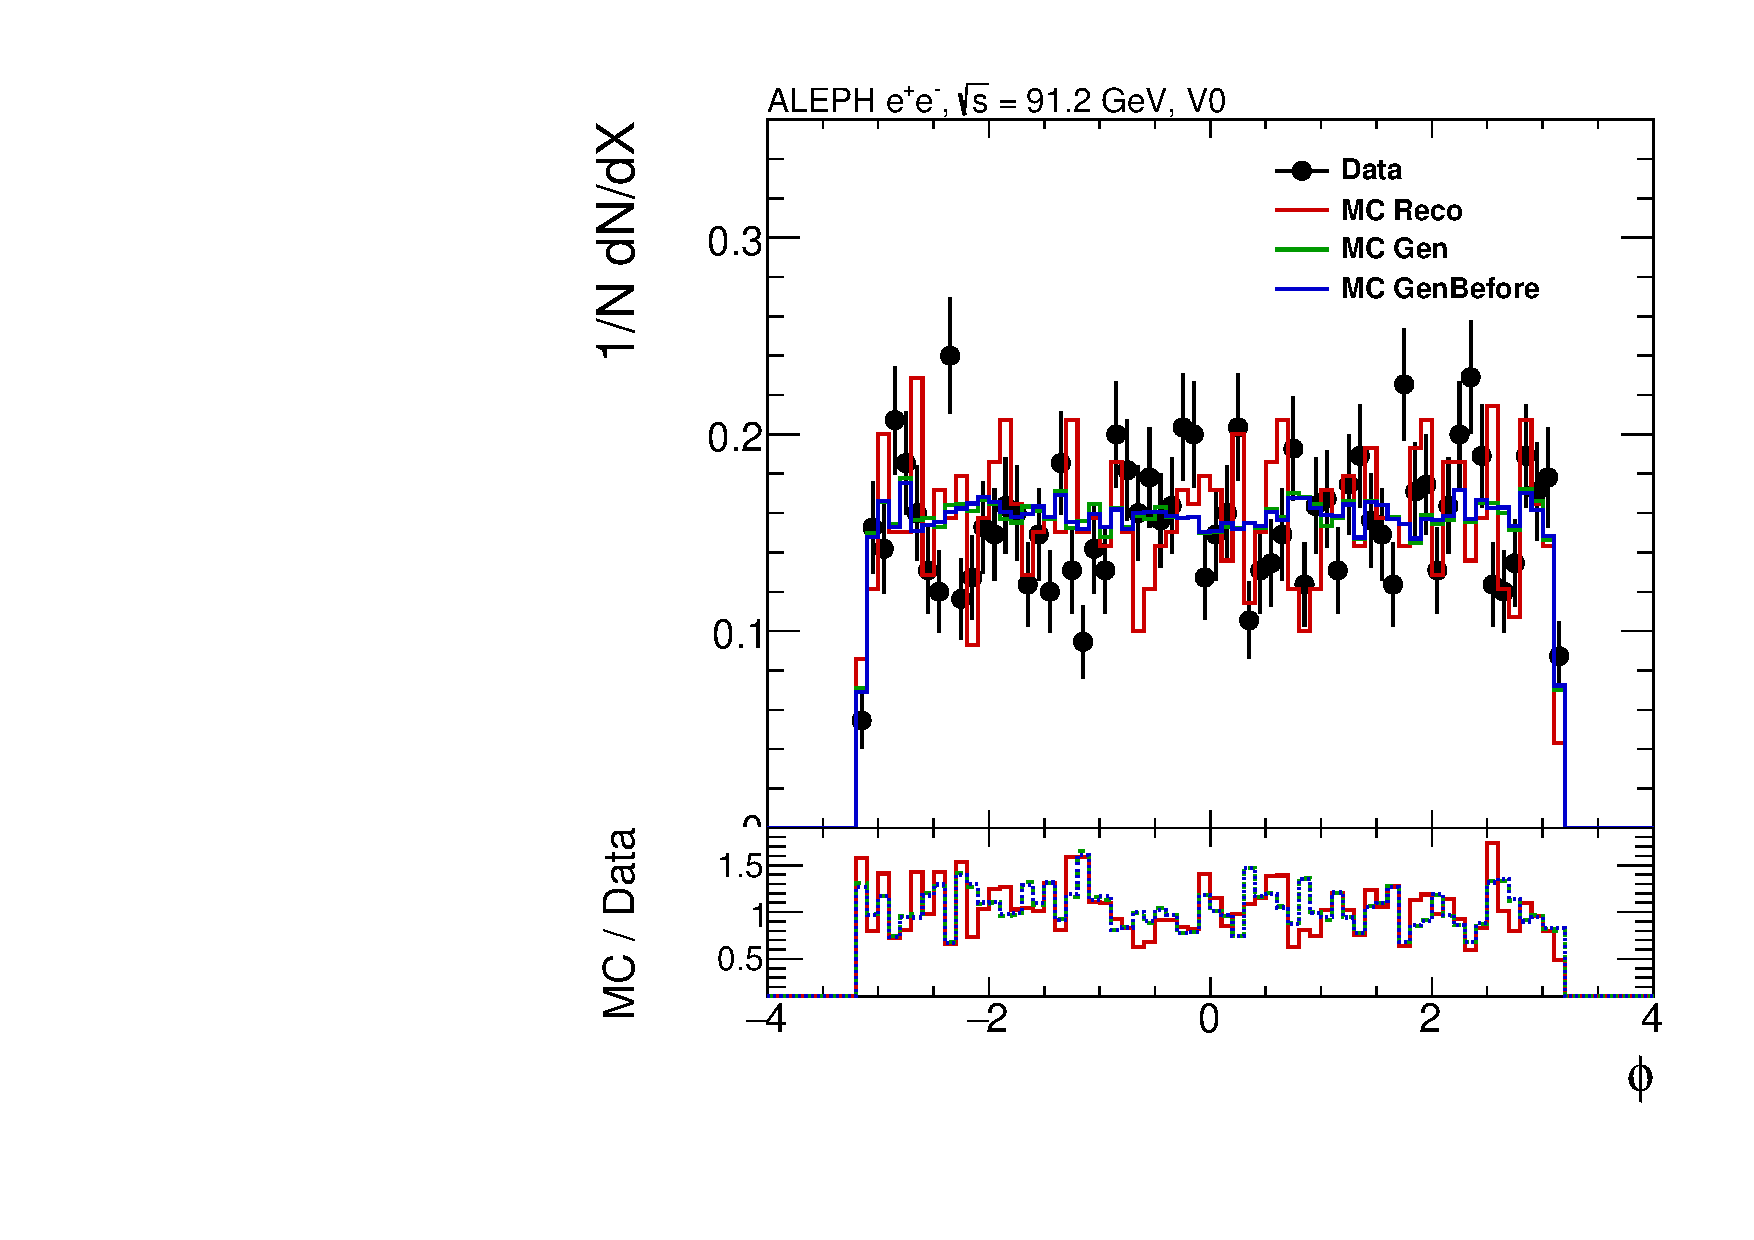
\includegraphics[width=0.325\textwidth]{../Studies/PreliminaryResult/2026-02-17_thrust_iter5/pwflag_kinematics/pwflag3_phi.pdf}
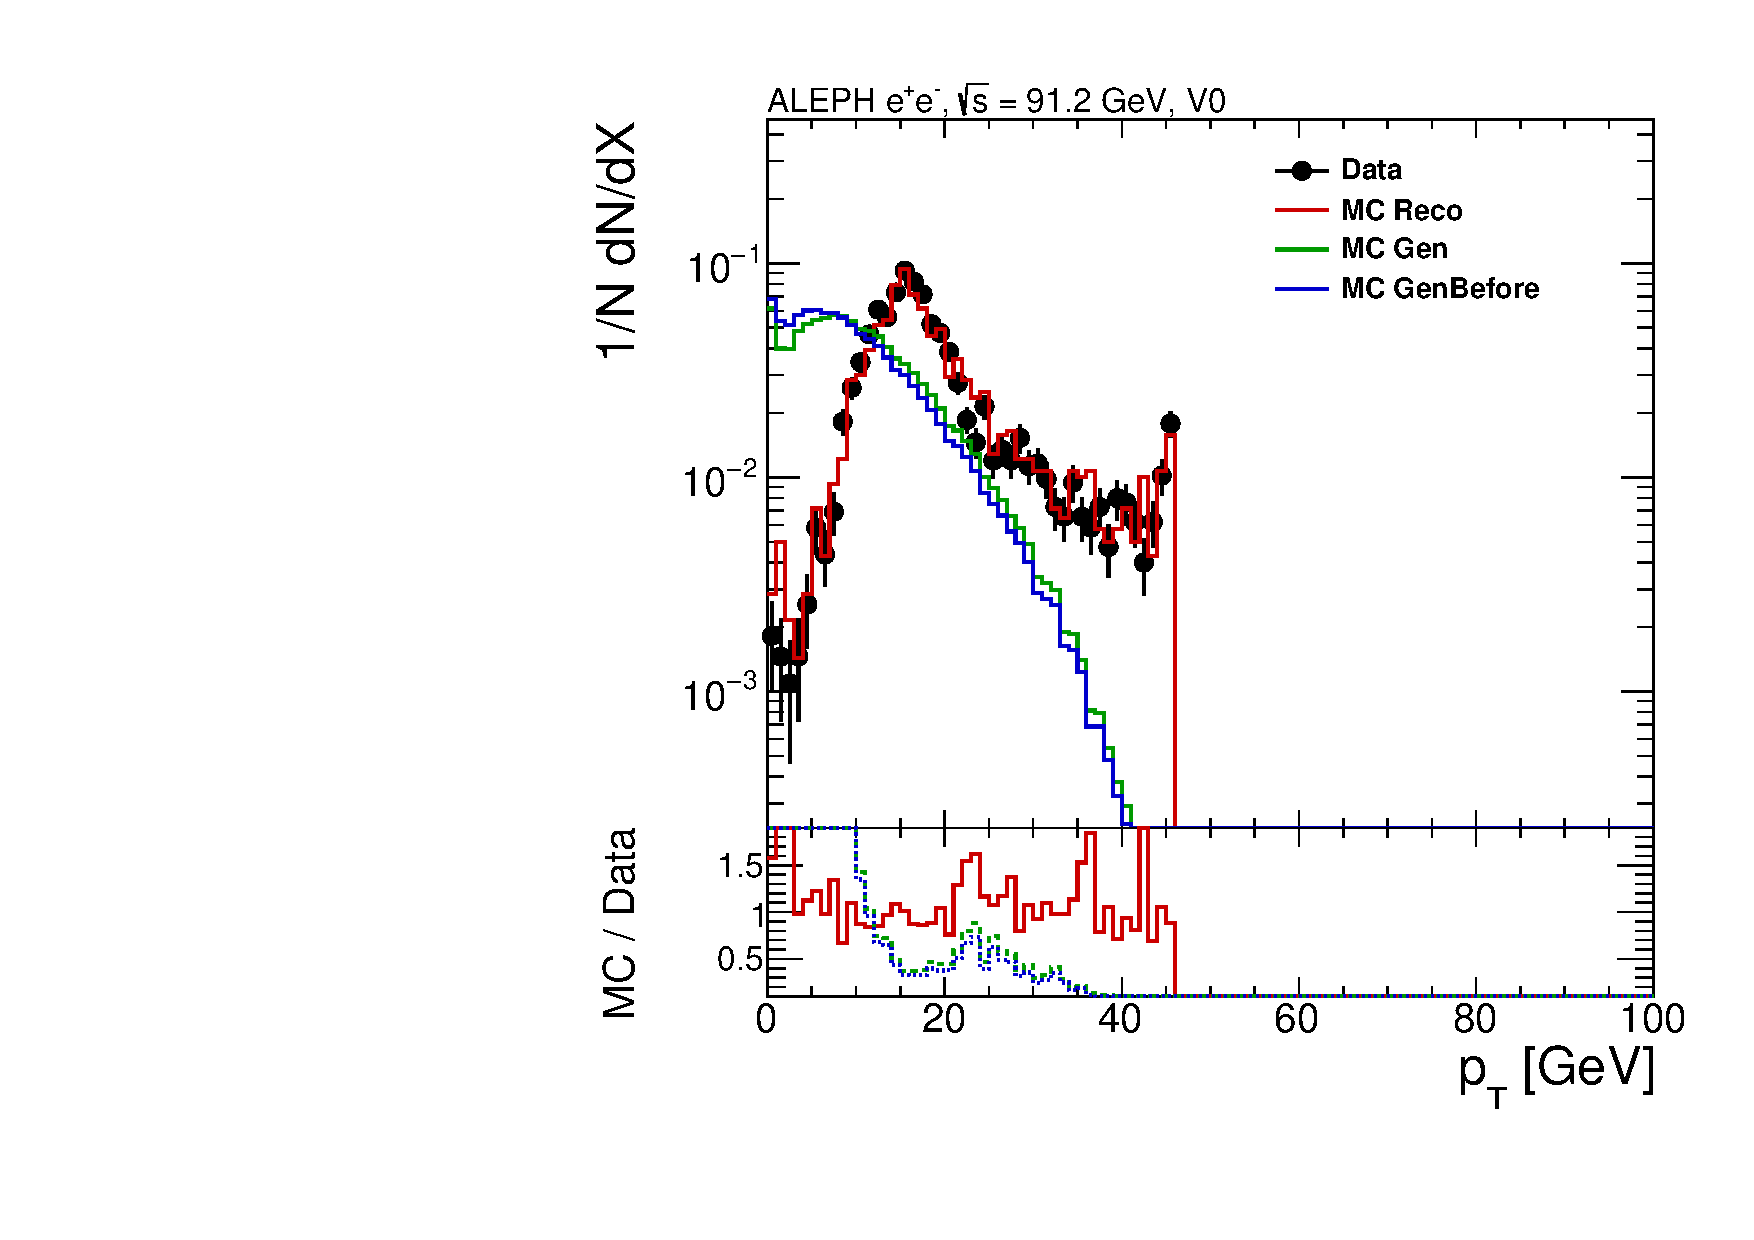
\includegraphics[width=0.325\textwidth]{../Studies/PreliminaryResult/2026-02-17_thrust_iter5/pwflag_kinematics/pwflag3_pt.pdf}
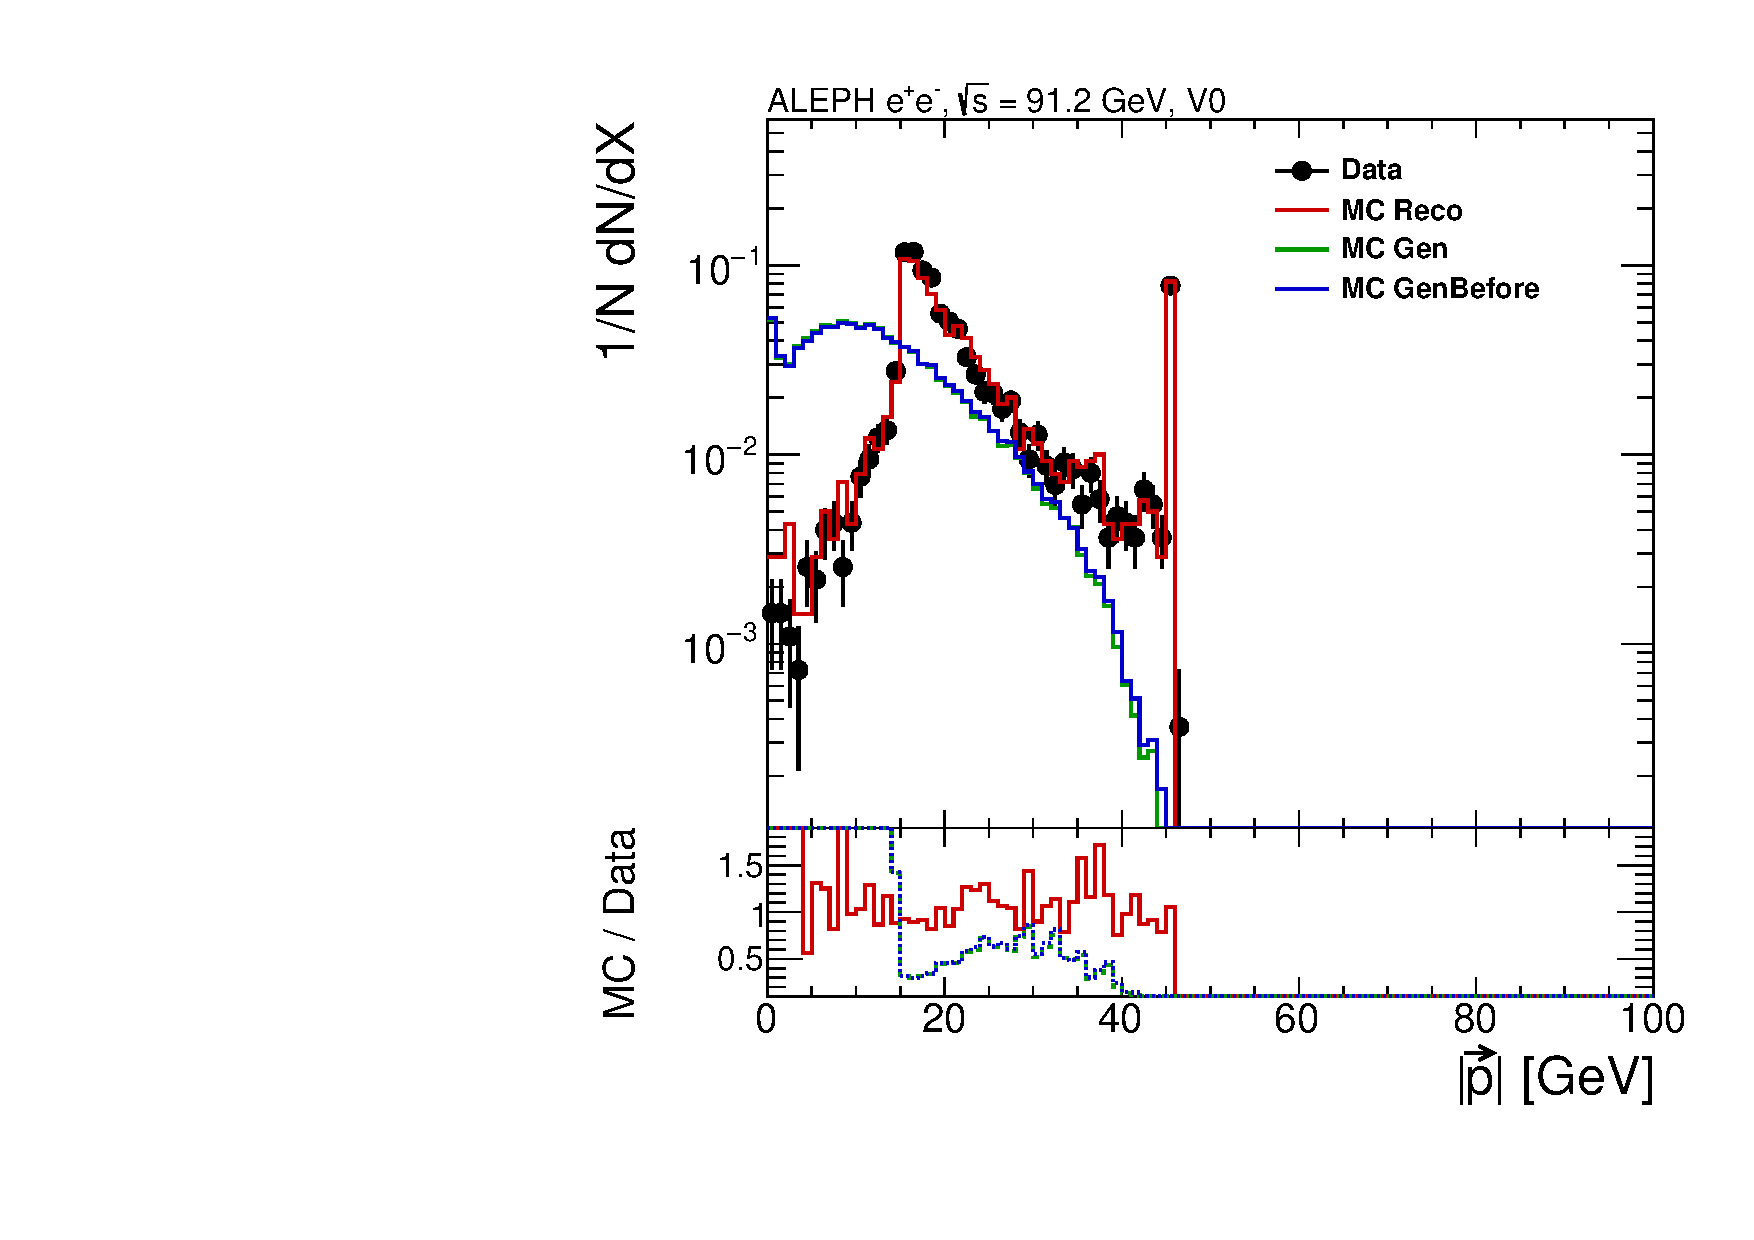
\includegraphics[width=0.325\textwidth]{../Studies/PreliminaryResult/2026-02-17_thrust_iter5/pwflag_kinematics/pwflag3_pmag.pdf}
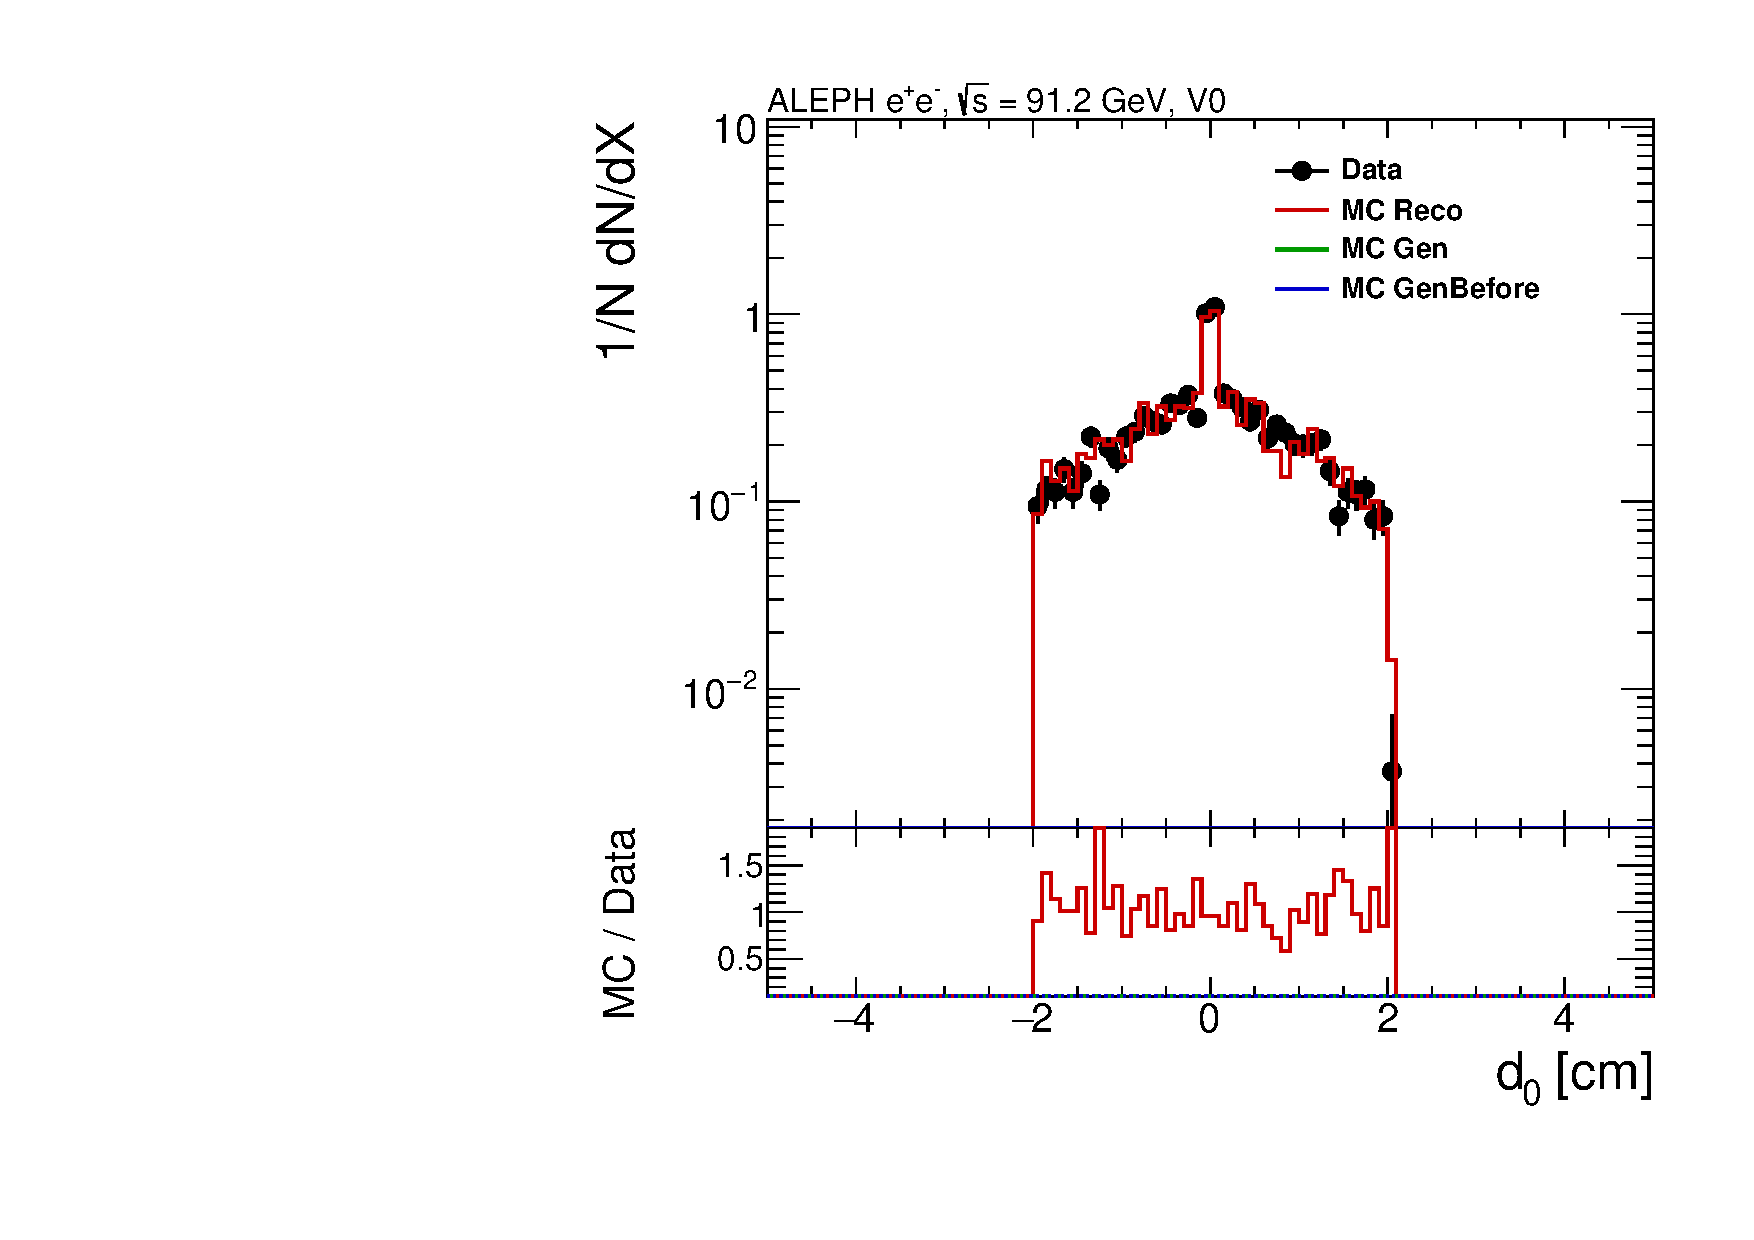
\includegraphics[width=0.325\textwidth]{../Studies/PreliminaryResult/2026-02-17_thrust_iter5/pwflag_kinematics/pwflag3_d0.pdf}
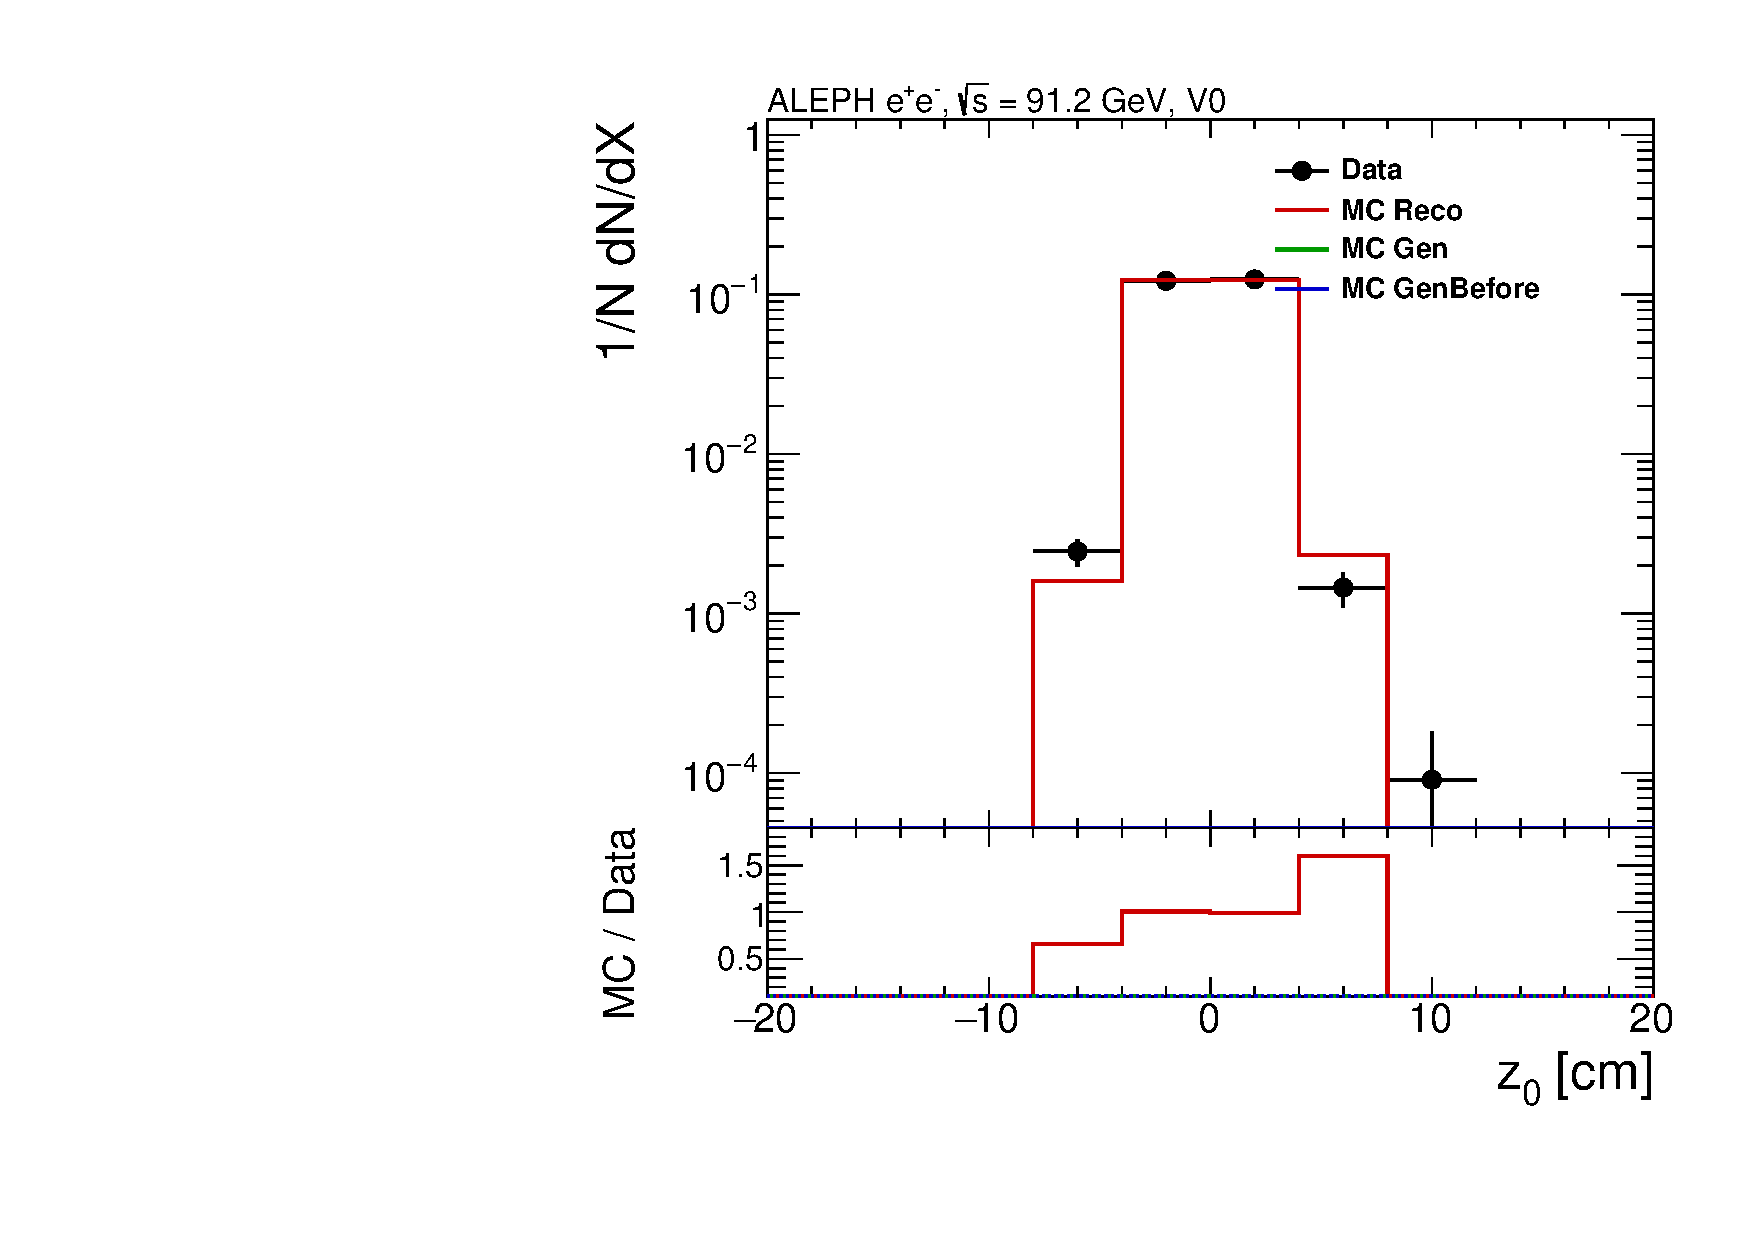
\includegraphics[width=0.325\textwidth]{../Studies/PreliminaryResult/2026-02-17_thrust_iter5/pwflag_kinematics/pwflag3_z0.pdf}
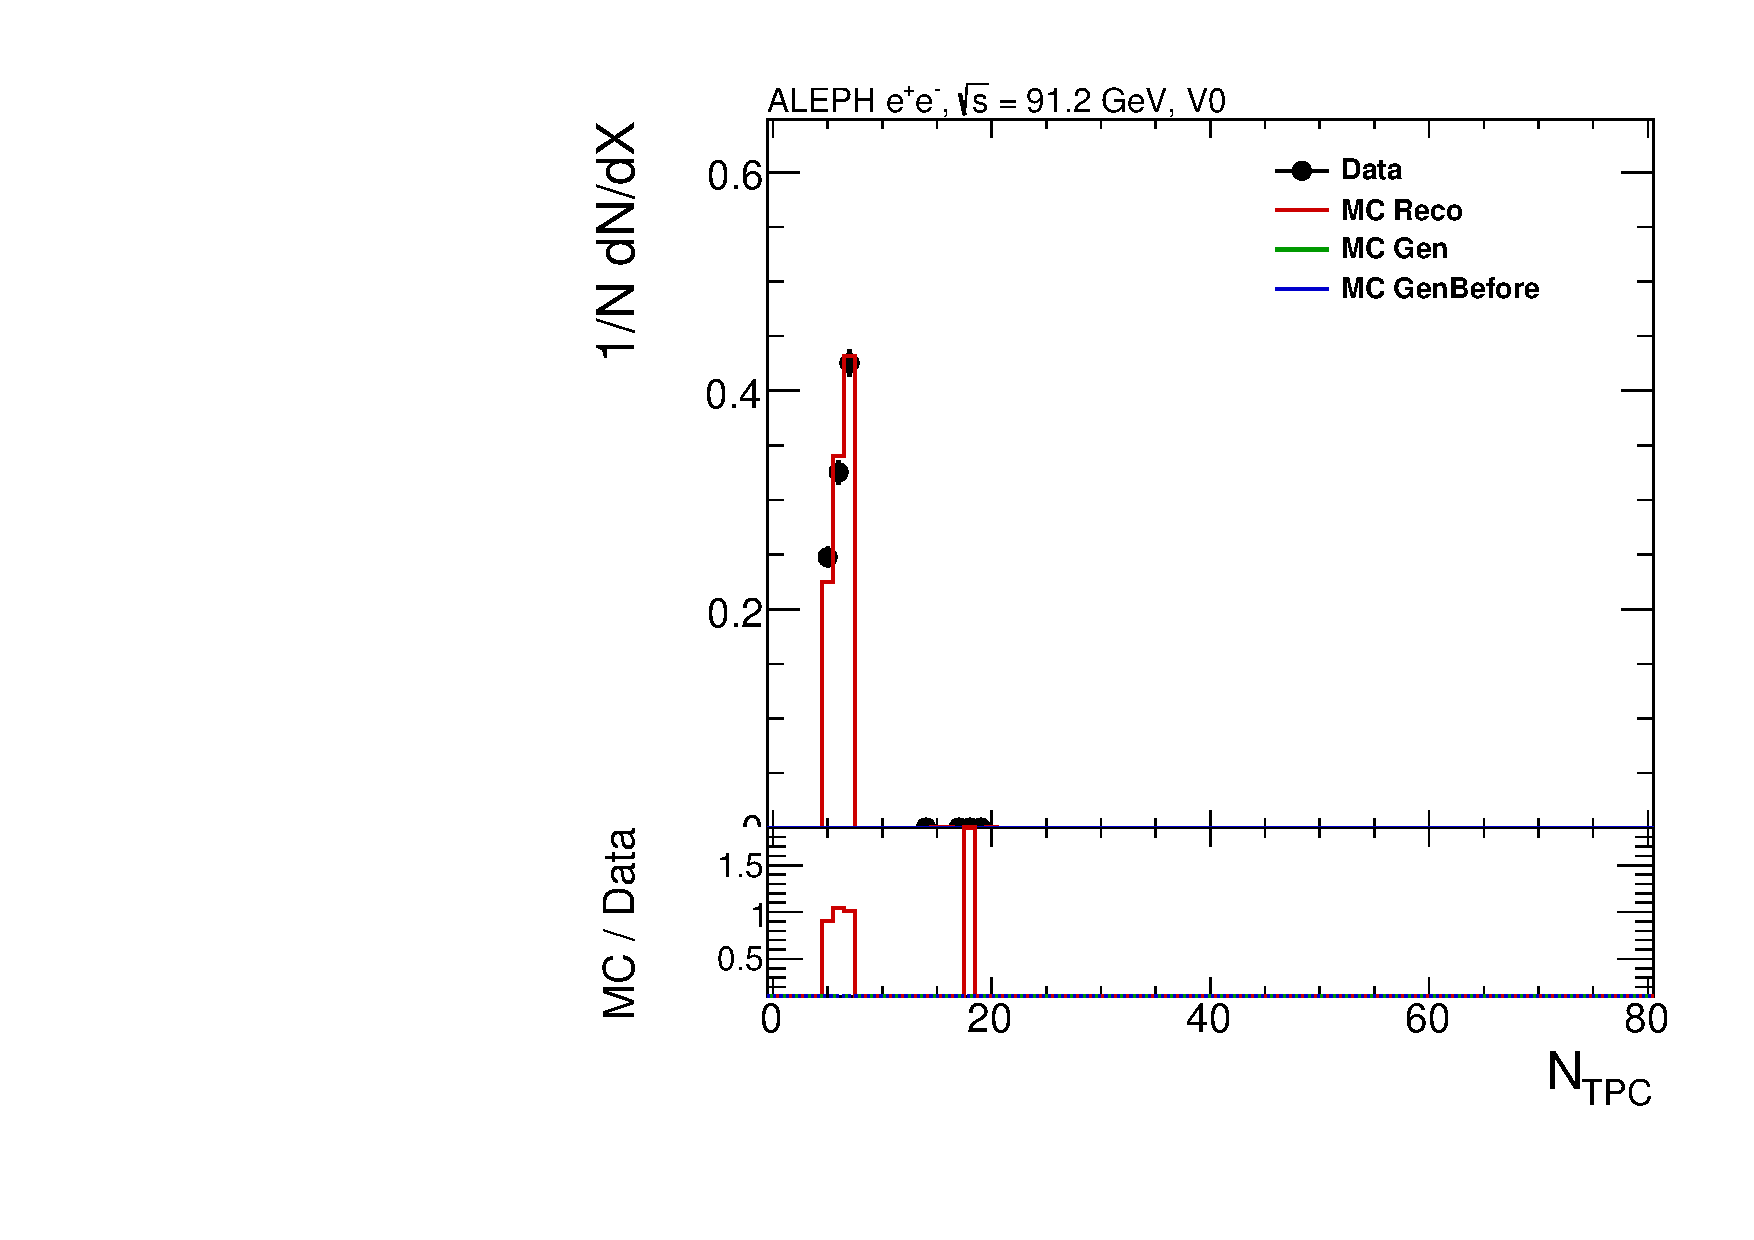
\includegraphics[width=0.325\textwidth]{../Studies/PreliminaryResult/2026-02-17_thrust_iter5/pwflag_kinematics/pwflag3_ntpc.pdf}
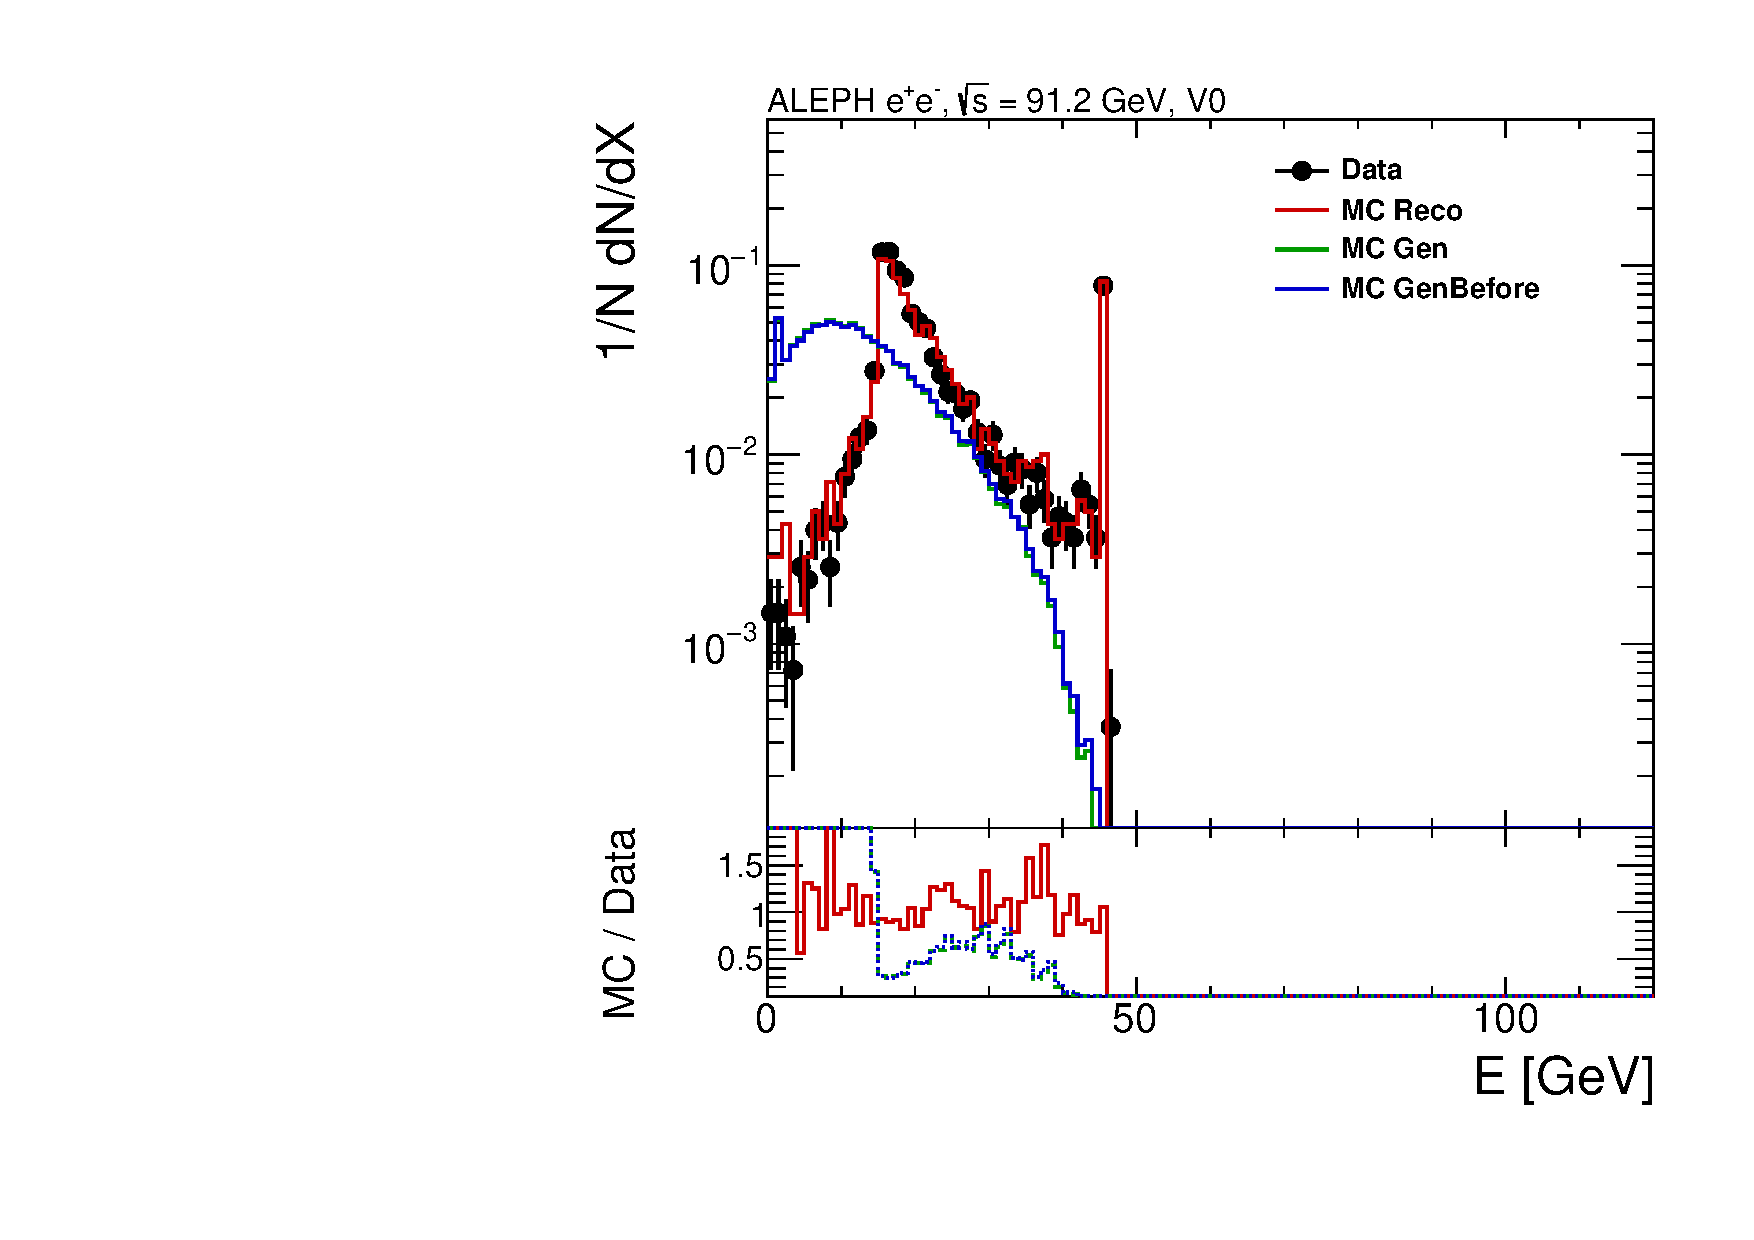
\includegraphics[width=0.325\textwidth]{../Studies/PreliminaryResult/2026-02-17_thrust_iter5/pwflag_kinematics/pwflag3_energy.pdf}
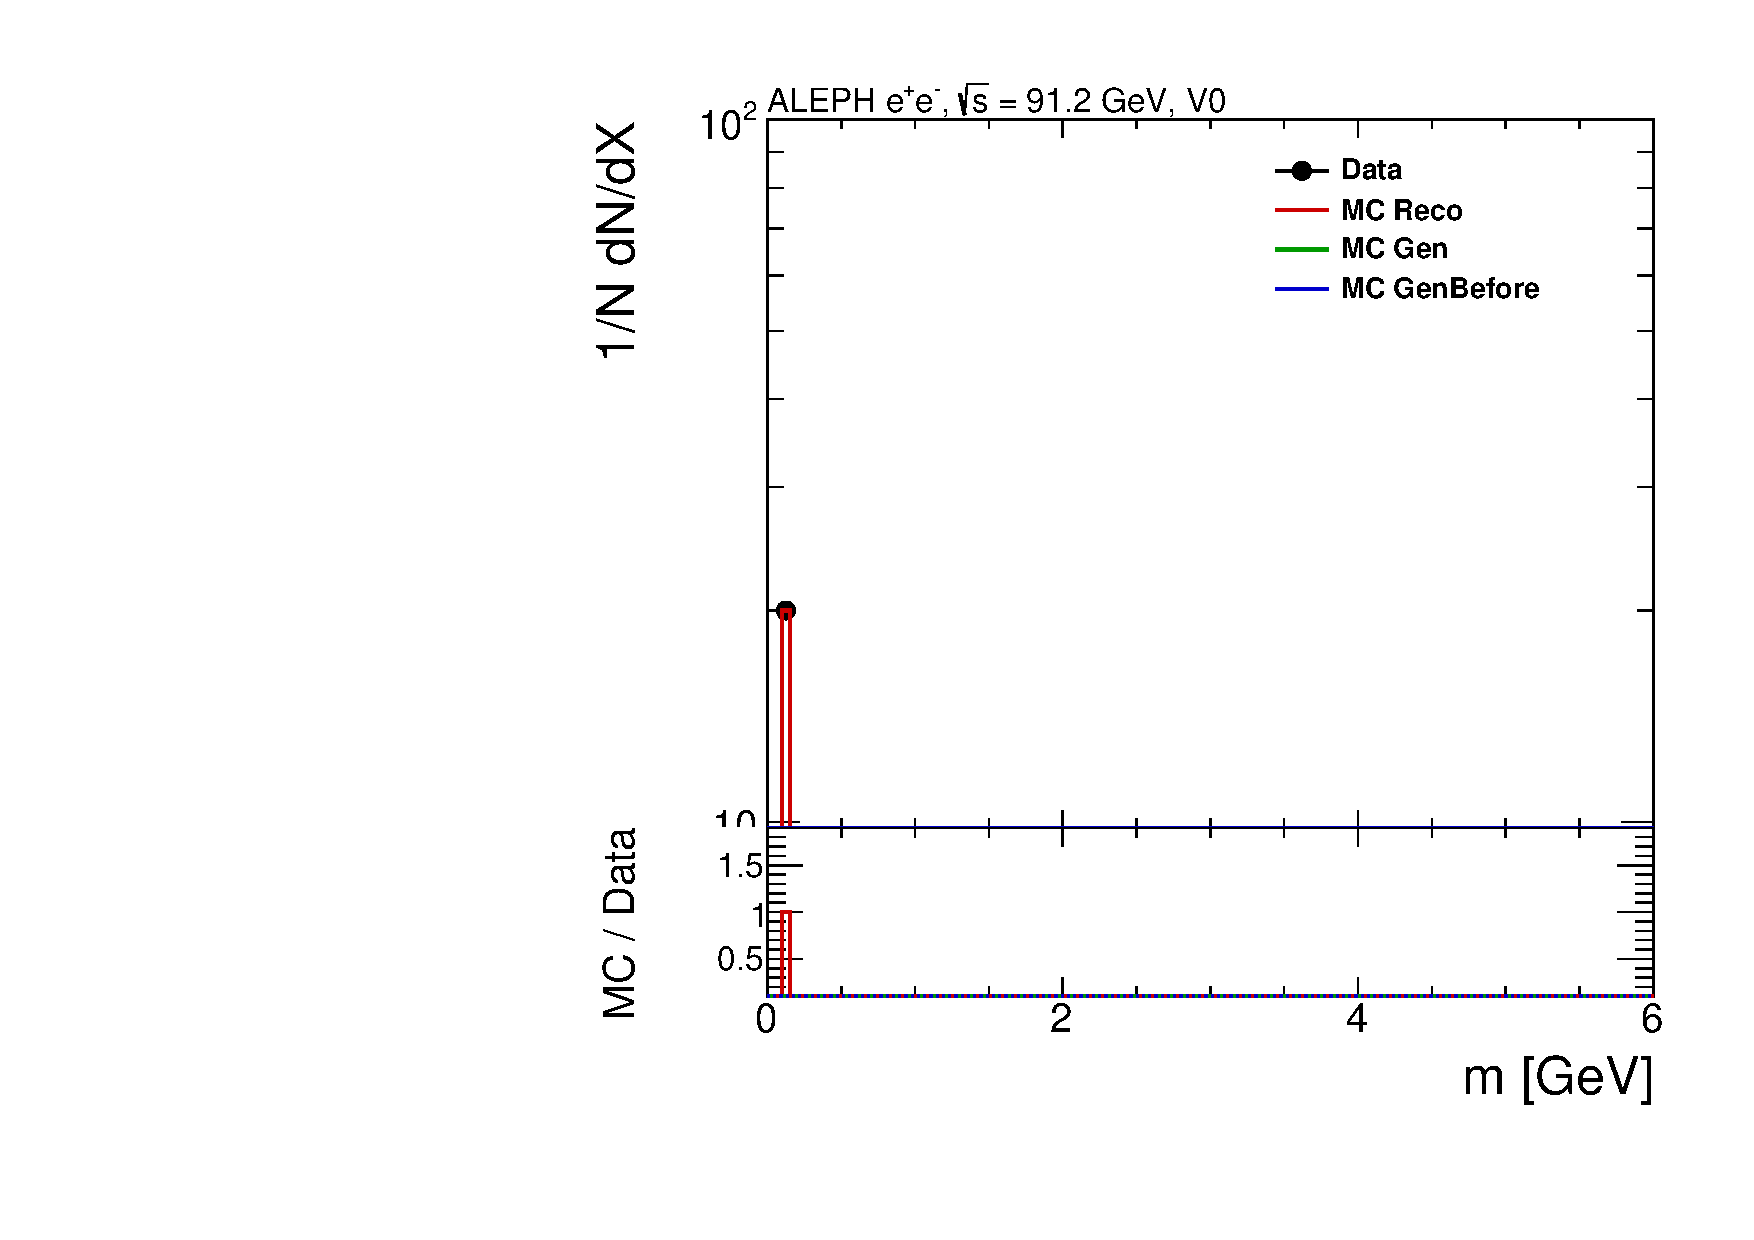
\includegraphics[width=0.325\textwidth]{../Studies/PreliminaryResult/2026-02-17_thrust_iter5/pwflag_kinematics/pwflag3_mass.pdf}
\caption{Complete \texttt{pwflag}=3 kinematic set.}
\label{fig:pwflag3_full}
\end{figure}

\noindent
Figure~\ref{fig:pwflag3_full} begins the neutral-object categories, where angular and energy
modeling are especially relevant for visible-energy flow in thrust reconstruction. For this
category, the energy spectrum and angular acceptance are the primary physics handles for event
shape modeling, while the track-like quantities provide consistency checks of the archived object
classification. Agreement in this panel supports a controlled transfer of neutral energy flow into
the unfolded thrust response.

\begin{figure}[t!]
\centering
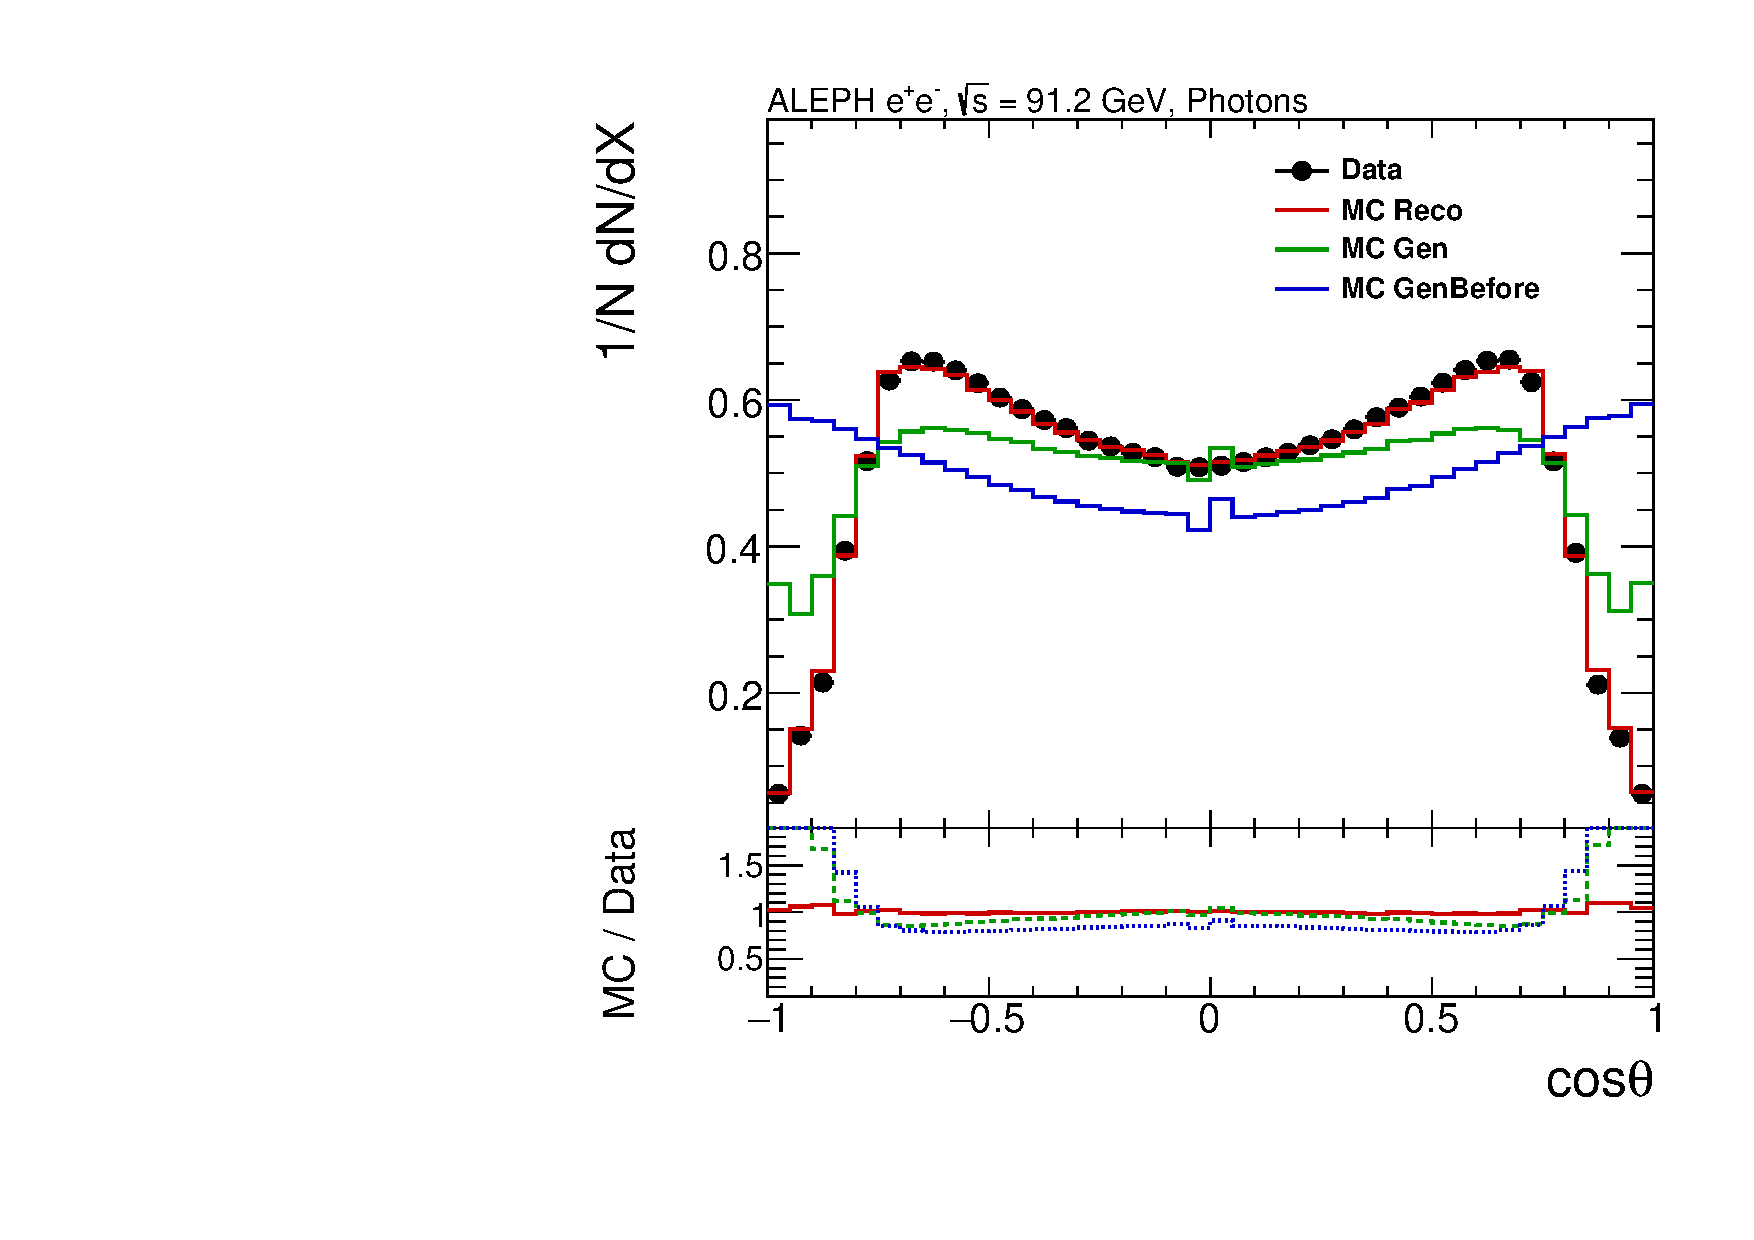
\includegraphics[width=0.325\textwidth]{../Studies/PreliminaryResult/2026-02-17_thrust_iter5/pwflag_kinematics/pwflag4_cosTheta.pdf}
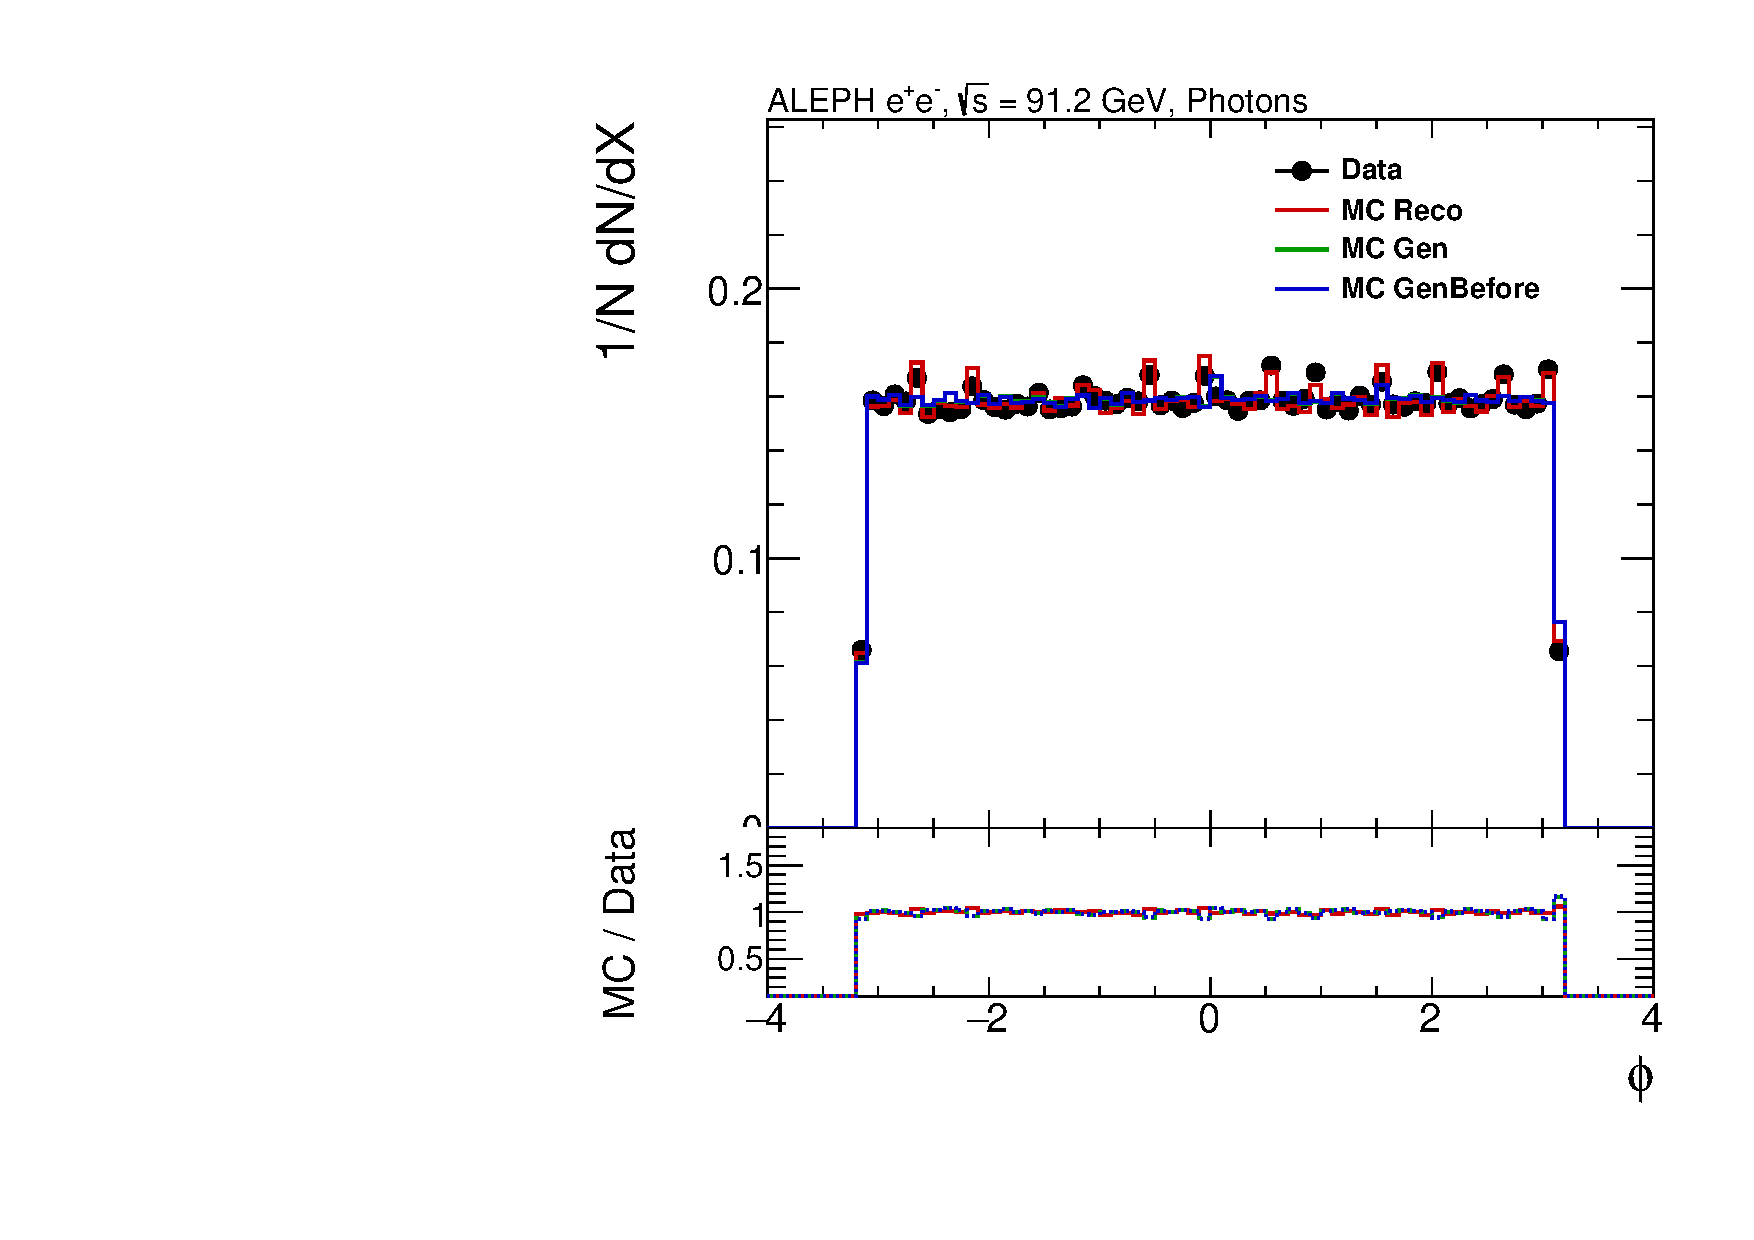
\includegraphics[width=0.325\textwidth]{../Studies/PreliminaryResult/2026-02-17_thrust_iter5/pwflag_kinematics/pwflag4_phi.pdf}
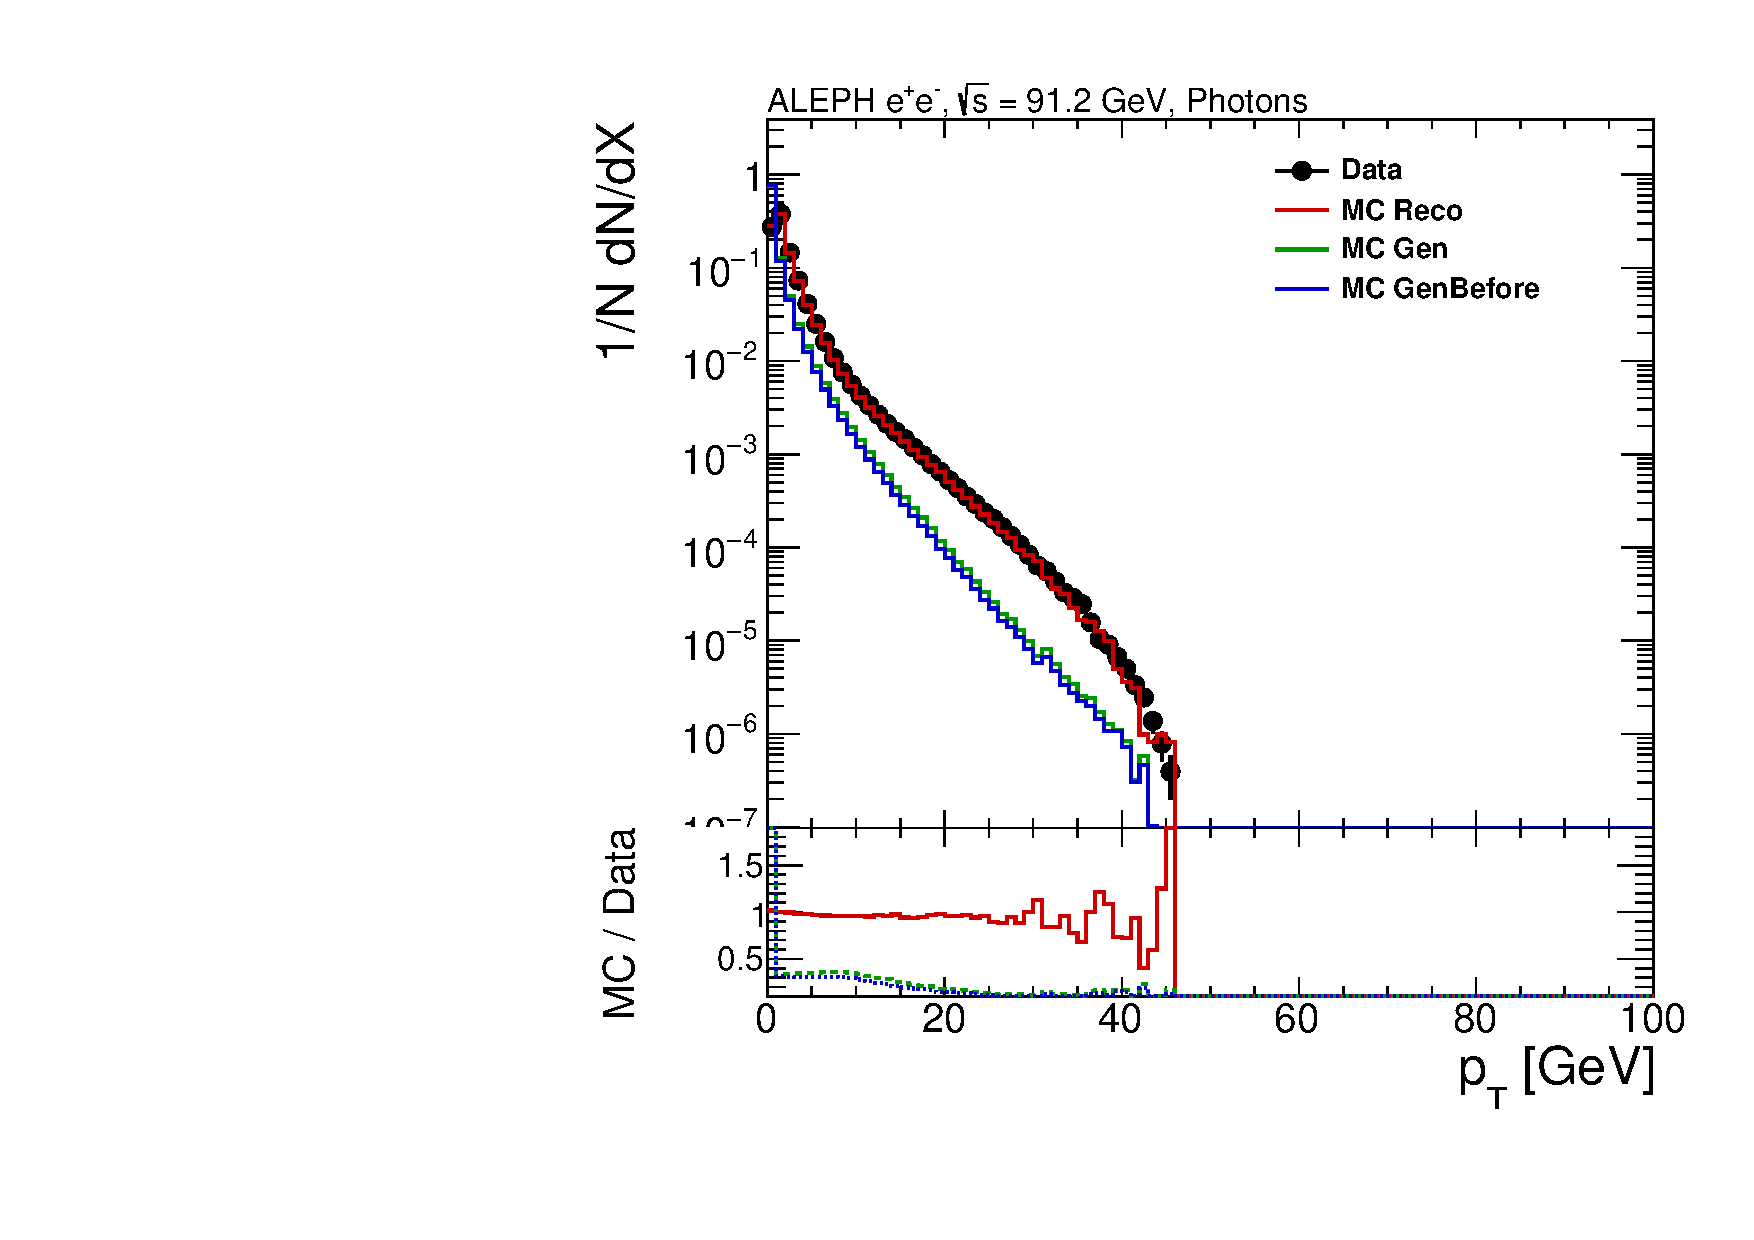
\includegraphics[width=0.325\textwidth]{../Studies/PreliminaryResult/2026-02-17_thrust_iter5/pwflag_kinematics/pwflag4_pt.pdf}
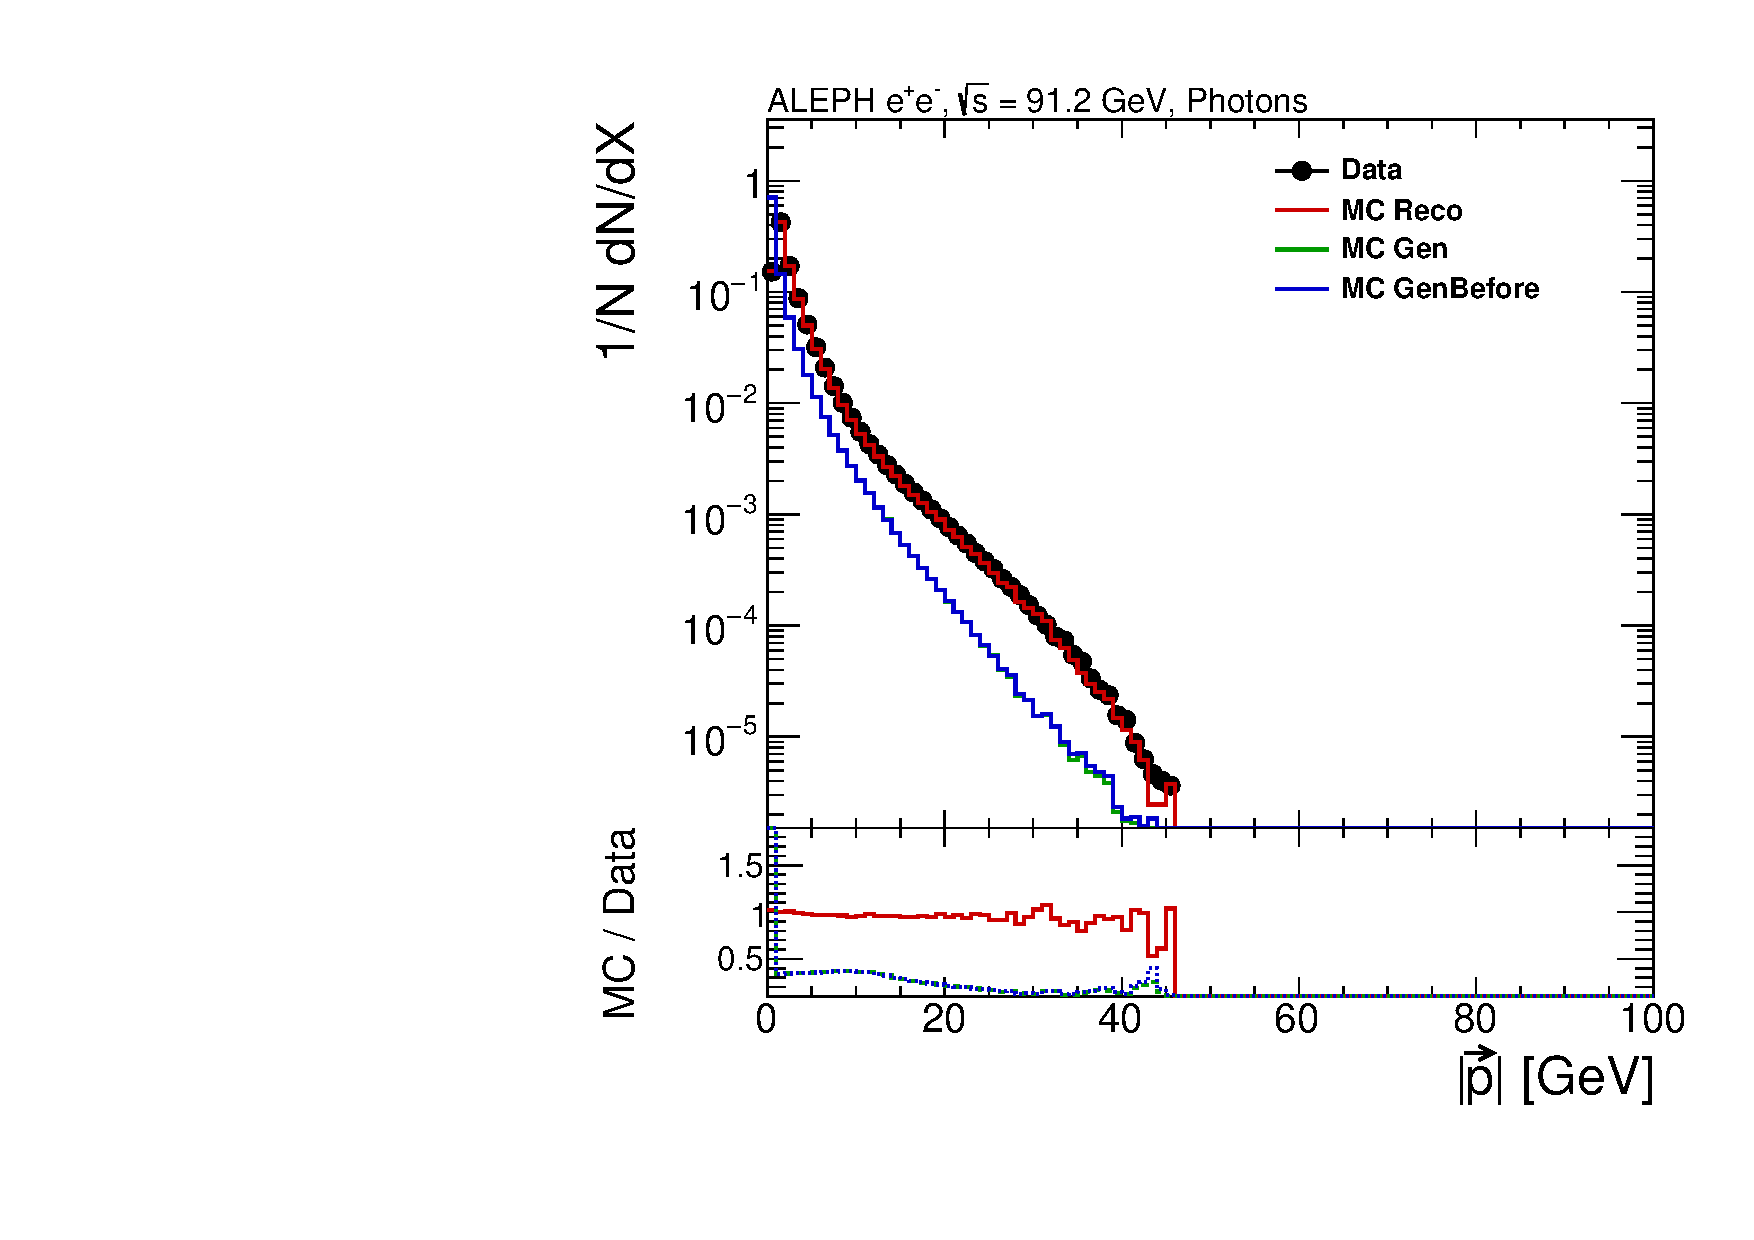
\includegraphics[width=0.325\textwidth]{../Studies/PreliminaryResult/2026-02-17_thrust_iter5/pwflag_kinematics/pwflag4_pmag.pdf}
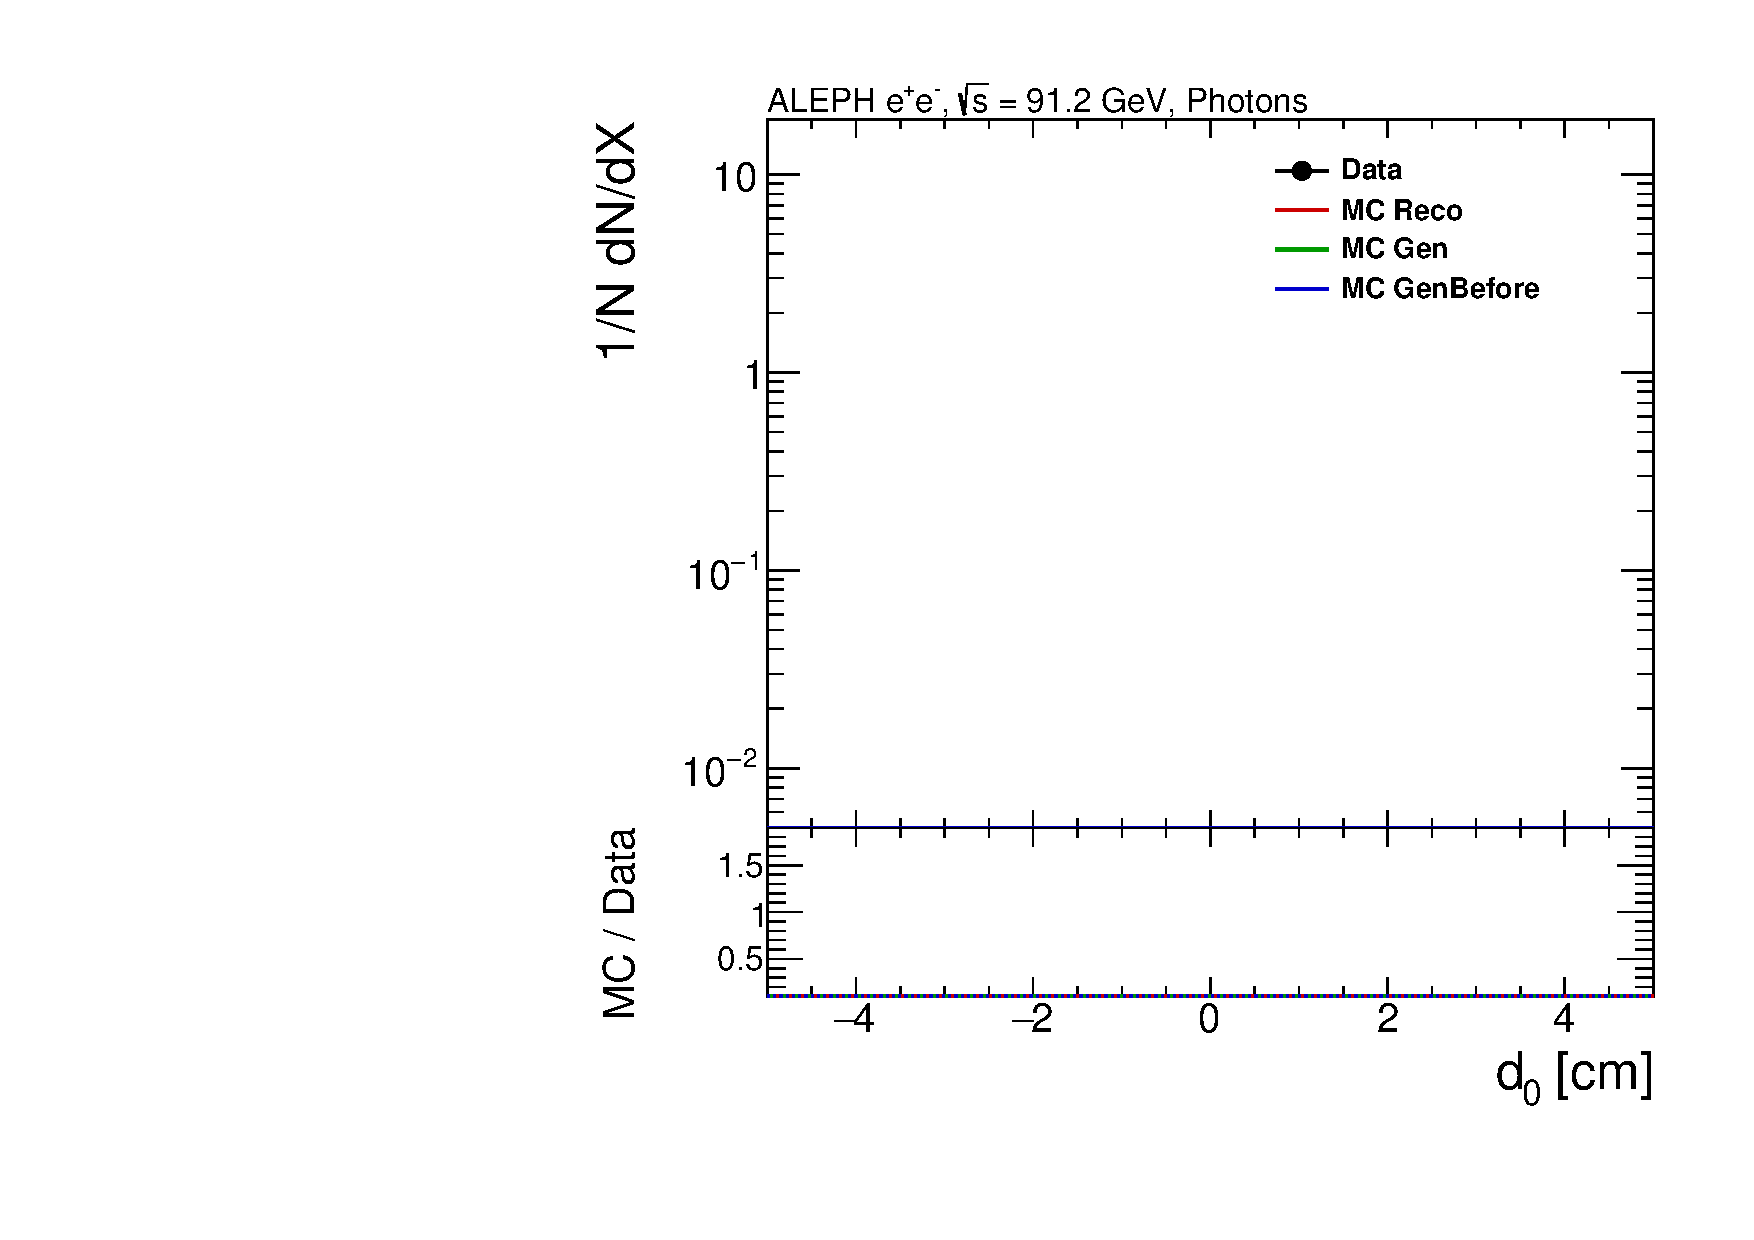
\includegraphics[width=0.325\textwidth]{../Studies/PreliminaryResult/2026-02-17_thrust_iter5/pwflag_kinematics/pwflag4_d0.pdf}
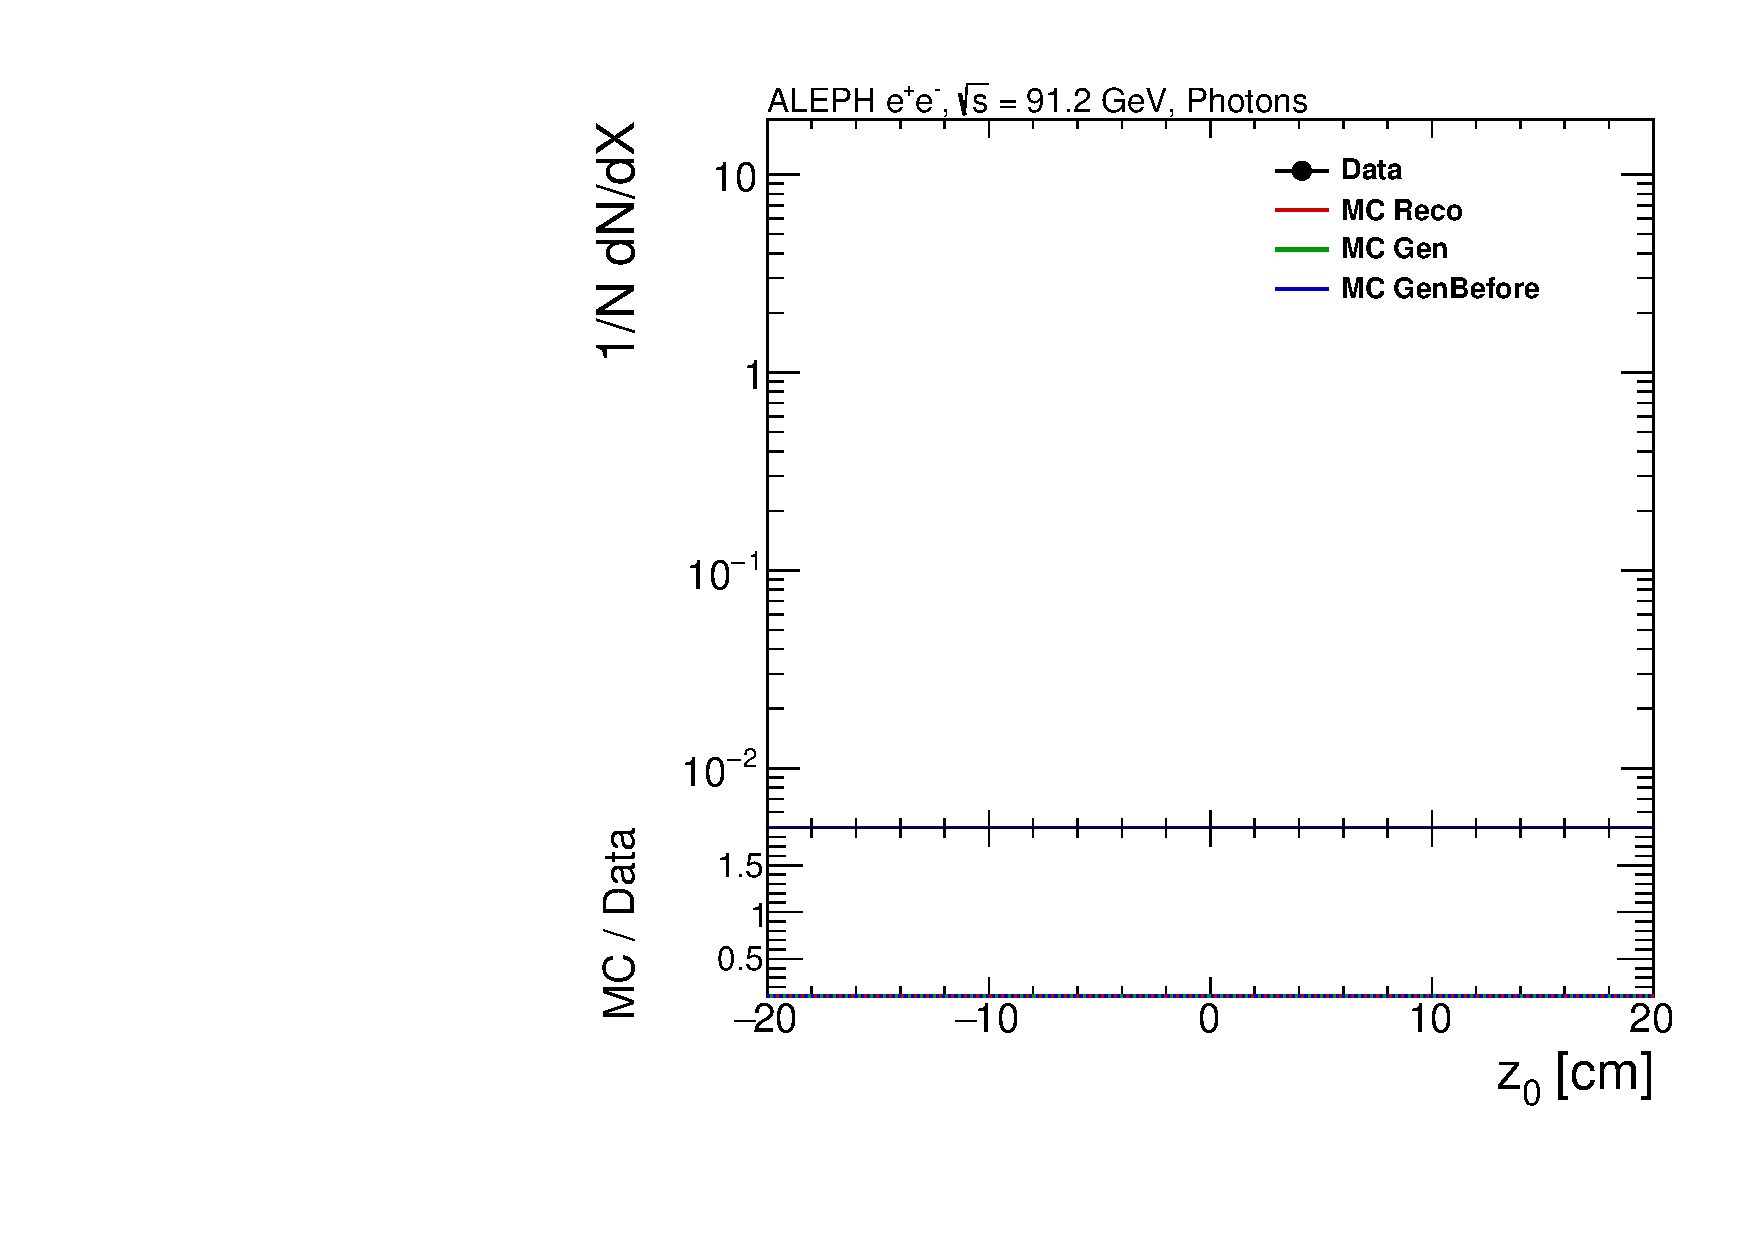
\includegraphics[width=0.325\textwidth]{../Studies/PreliminaryResult/2026-02-17_thrust_iter5/pwflag_kinematics/pwflag4_z0.pdf}
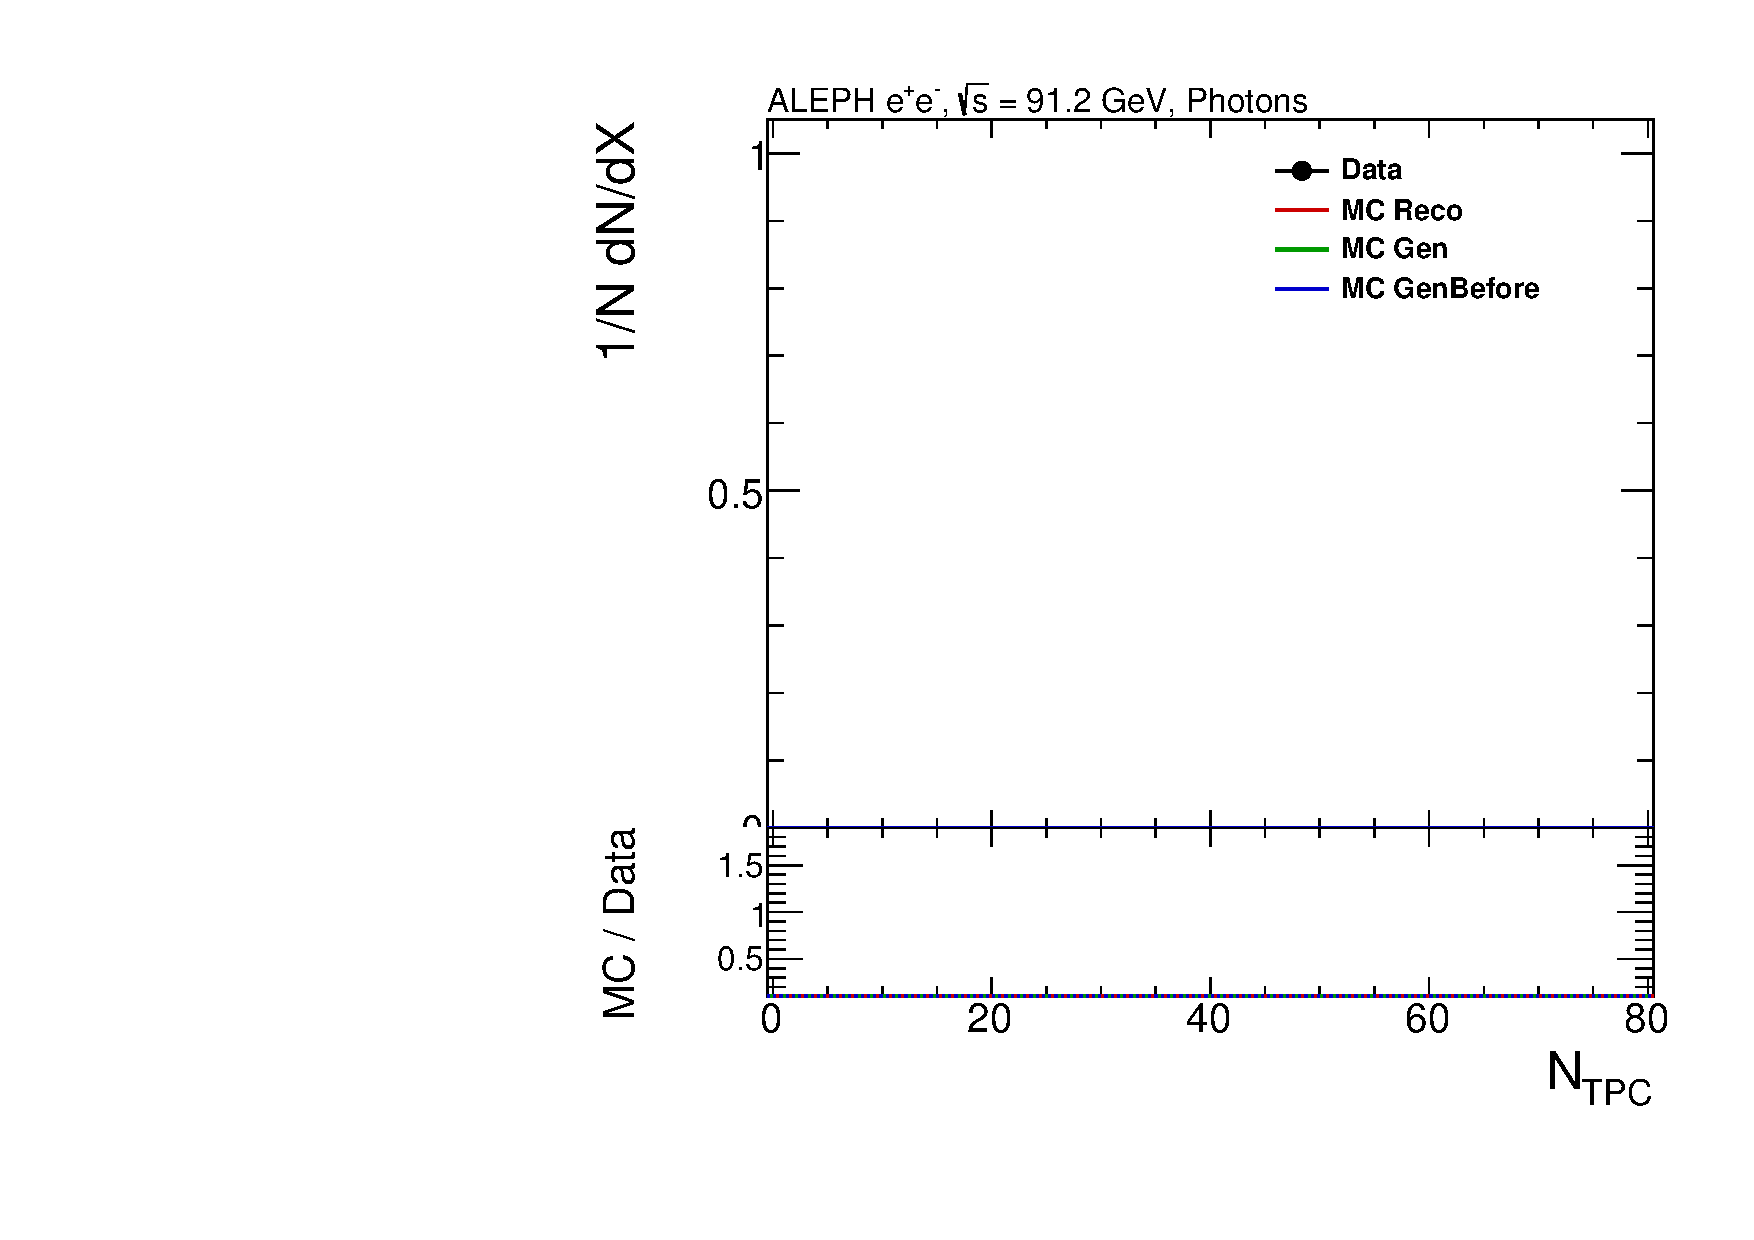
\includegraphics[width=0.325\textwidth]{../Studies/PreliminaryResult/2026-02-17_thrust_iter5/pwflag_kinematics/pwflag4_ntpc.pdf}
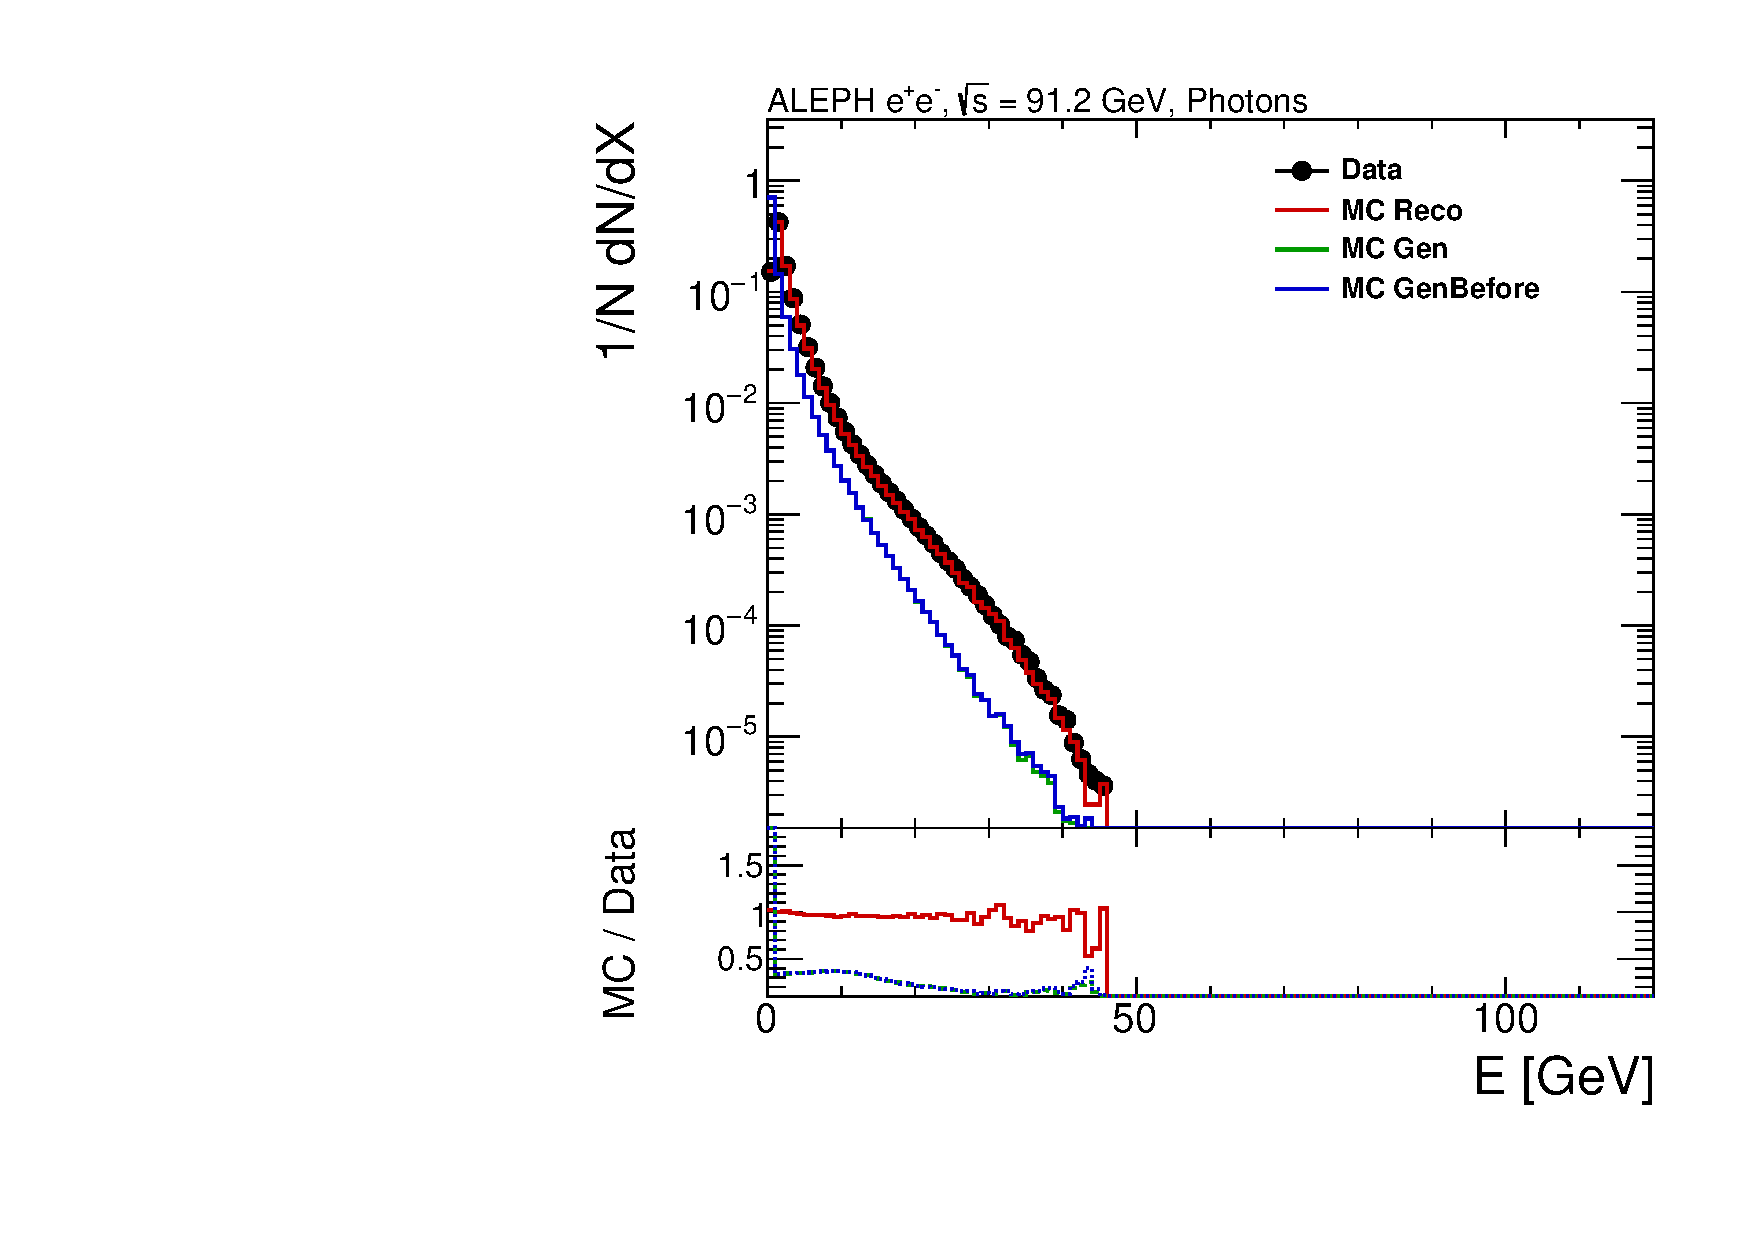
\includegraphics[width=0.325\textwidth]{../Studies/PreliminaryResult/2026-02-17_thrust_iter5/pwflag_kinematics/pwflag4_energy.pdf}
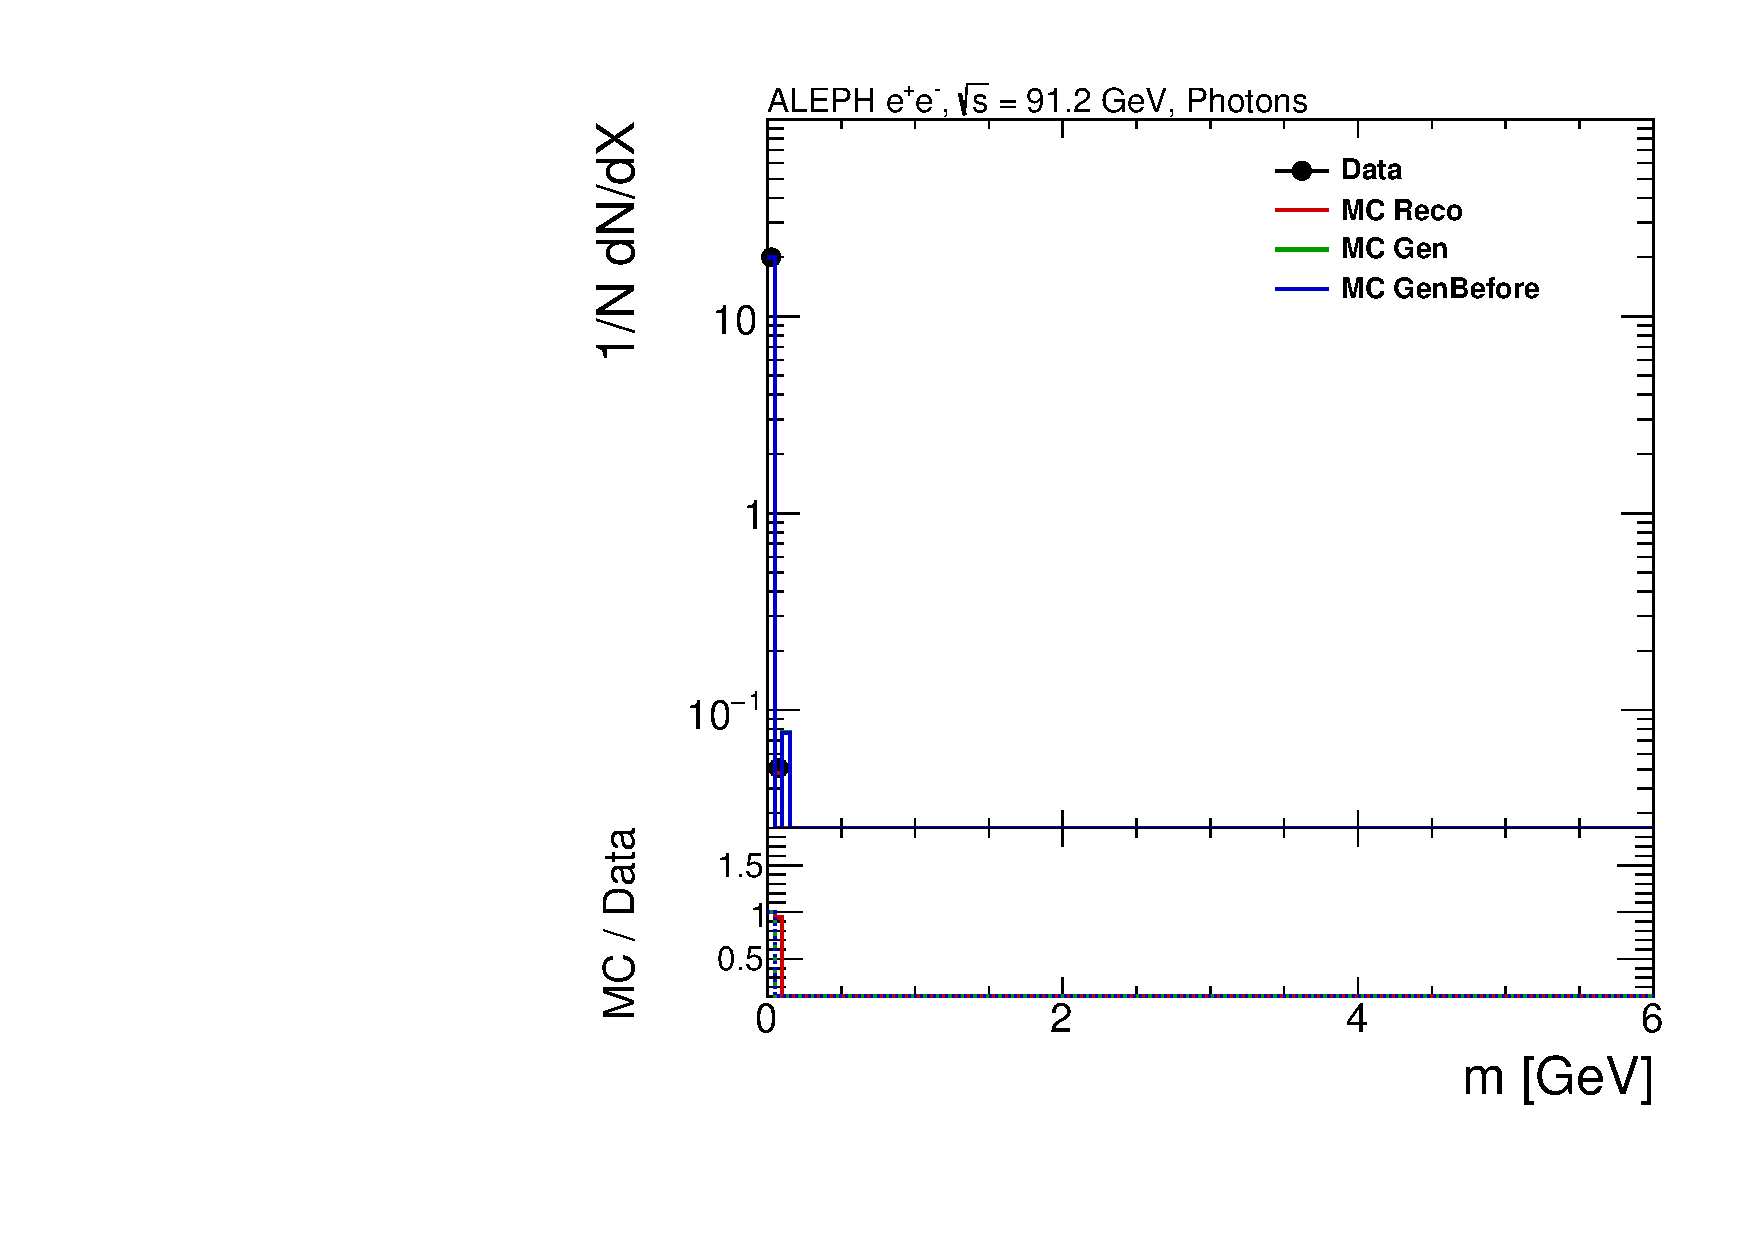
\includegraphics[width=0.325\textwidth]{../Studies/PreliminaryResult/2026-02-17_thrust_iter5/pwflag_kinematics/pwflag4_mass.pdf}
\caption{Complete \texttt{pwflag}=4 kinematic set.}
\label{fig:pwflag4_full}
\end{figure}

\noindent
Figure~\ref{fig:pwflag4_full} isolates photons, which probe neutral electromagnetic response and
its effect on event-shape normalization. The photon energy and angular spectra are especially
important because electromagnetic neutral energy contributes directly to visible event topology and
hemisphere energy balance. The observed data/MC consistency in the core region supports the
neutral-energy calibration assumptions used in the nominal unfolding and neutral-response
systematic variations.

\begin{figure}[t!]
\centering
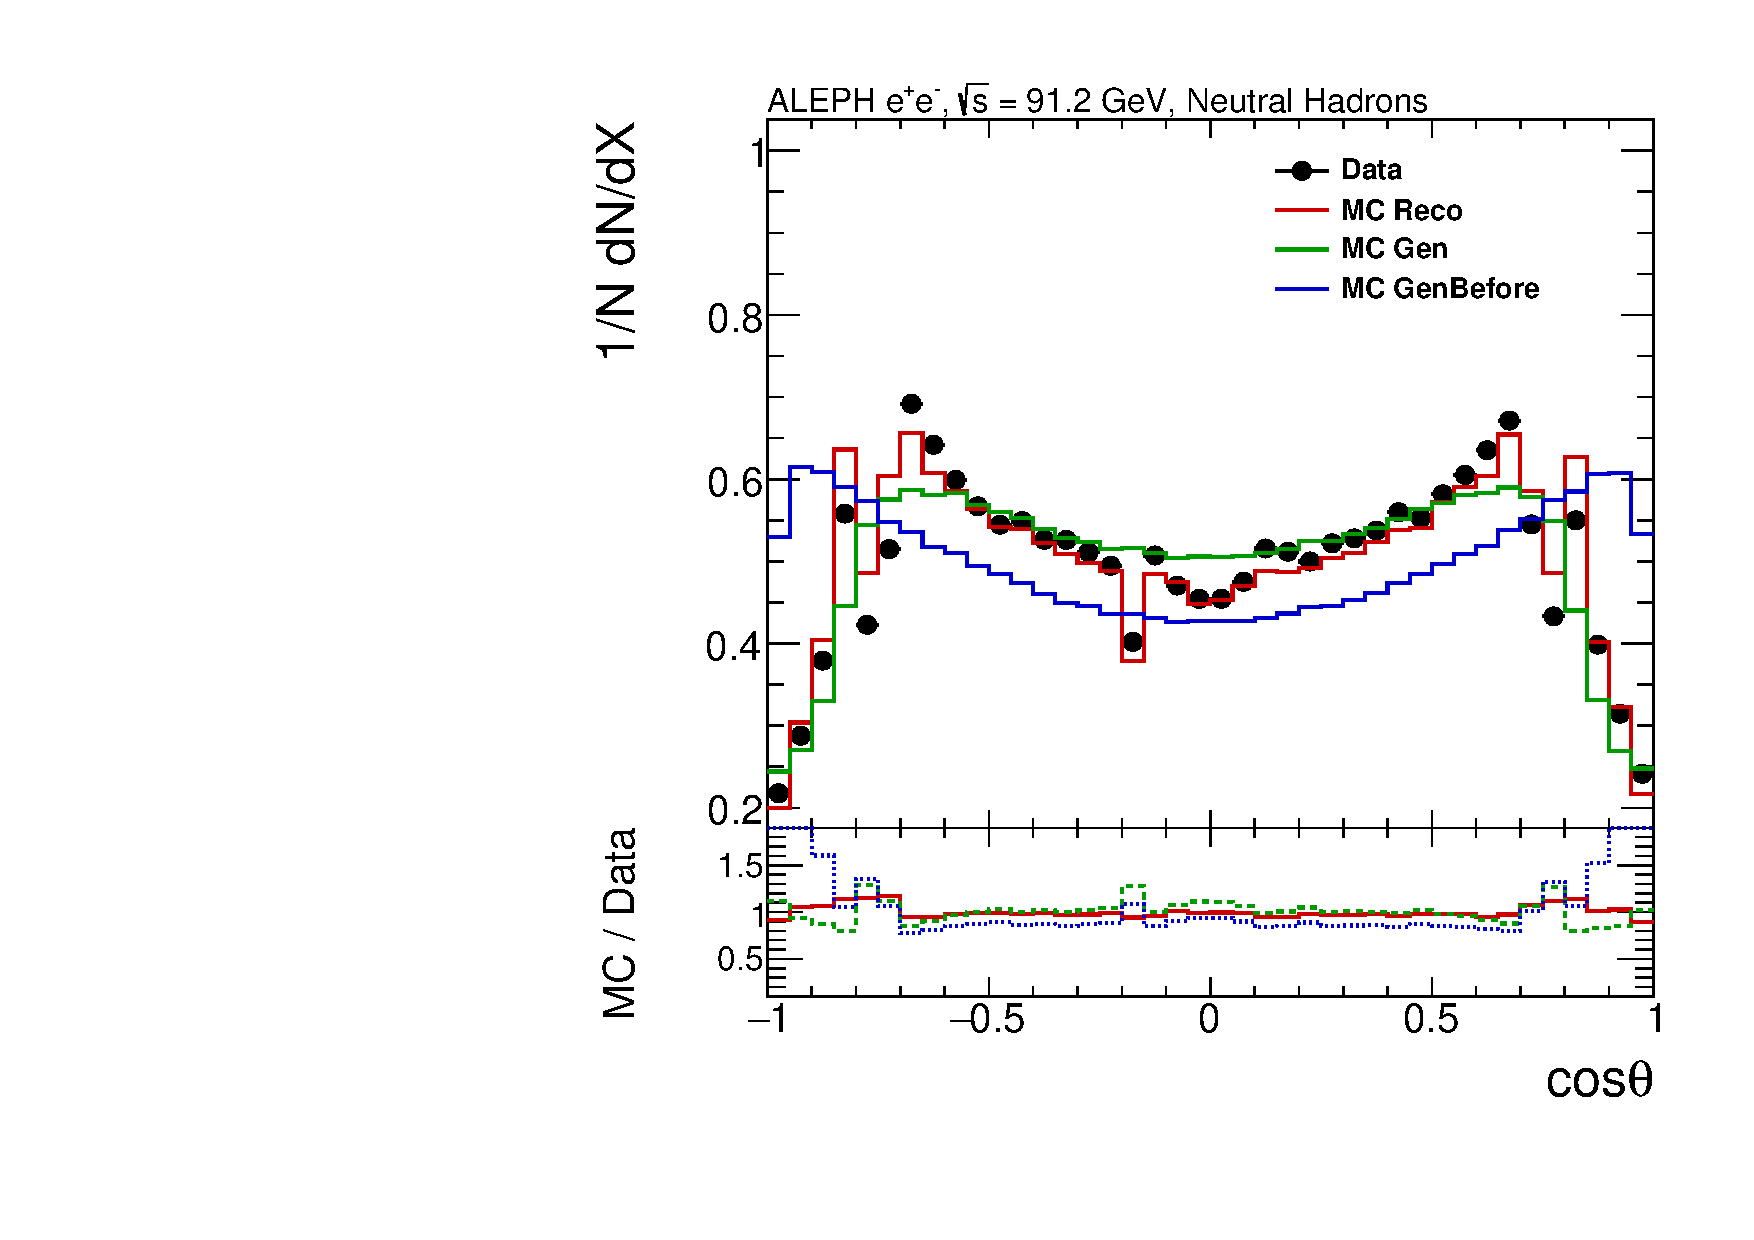
\includegraphics[width=0.325\textwidth]{../Studies/PreliminaryResult/2026-02-17_thrust_iter5/pwflag_kinematics/pwflag5_cosTheta.pdf}
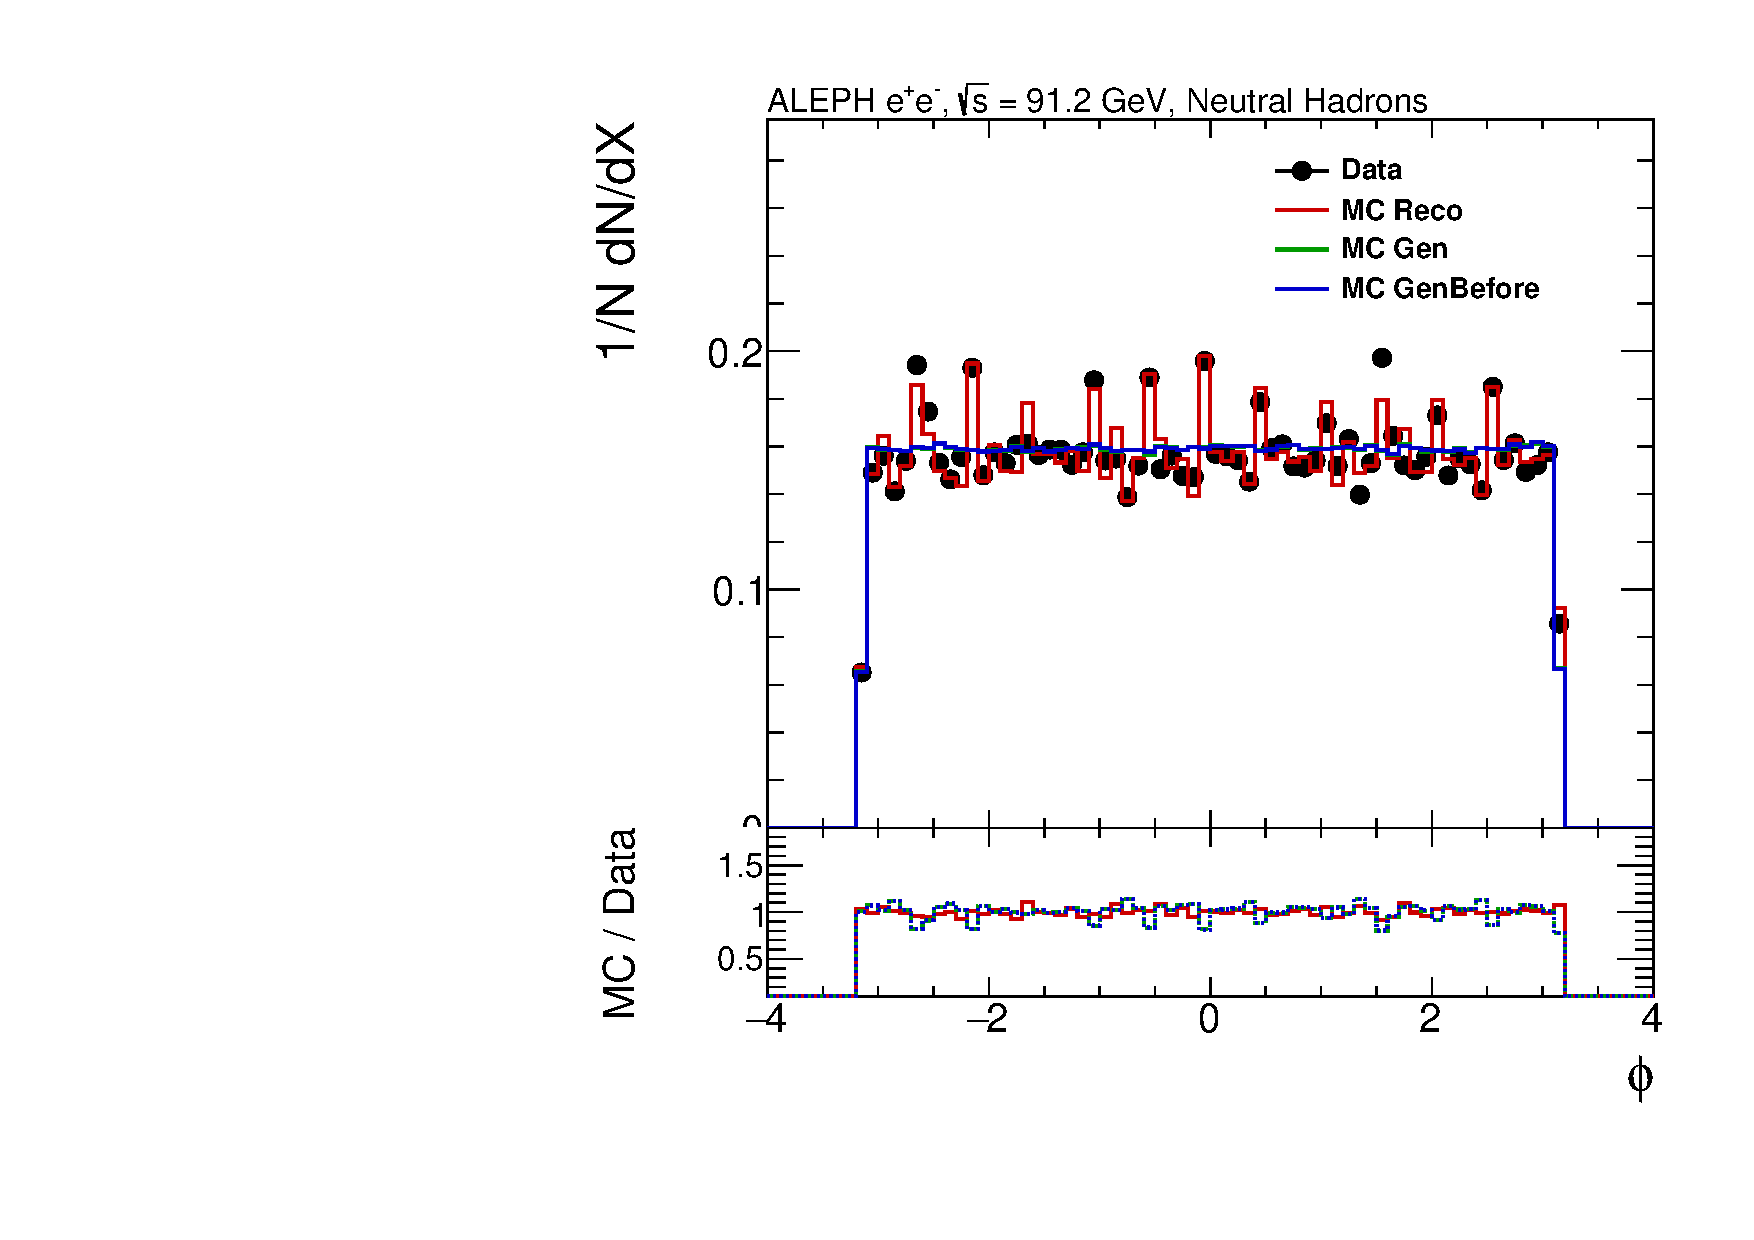
\includegraphics[width=0.325\textwidth]{../Studies/PreliminaryResult/2026-02-17_thrust_iter5/pwflag_kinematics/pwflag5_phi.pdf}
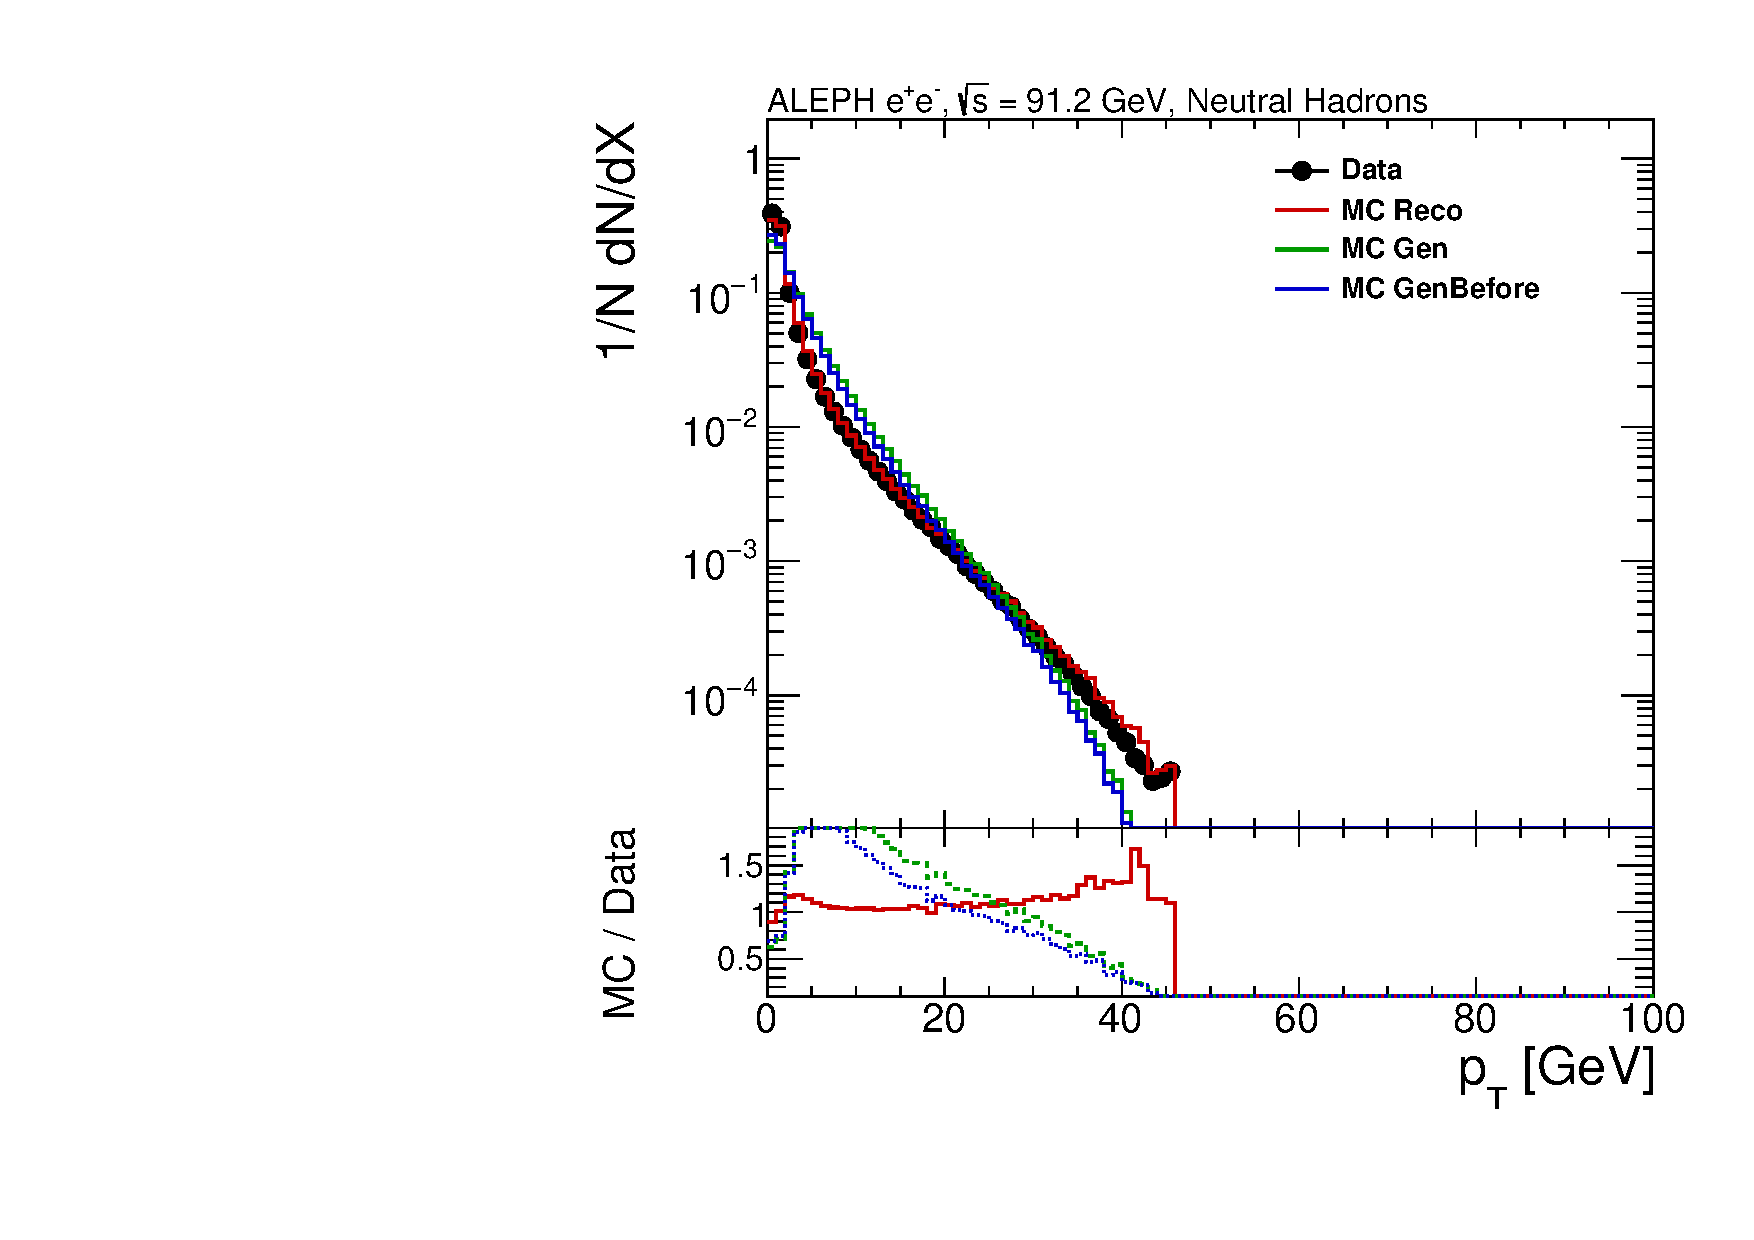
\includegraphics[width=0.325\textwidth]{../Studies/PreliminaryResult/2026-02-17_thrust_iter5/pwflag_kinematics/pwflag5_pt.pdf}
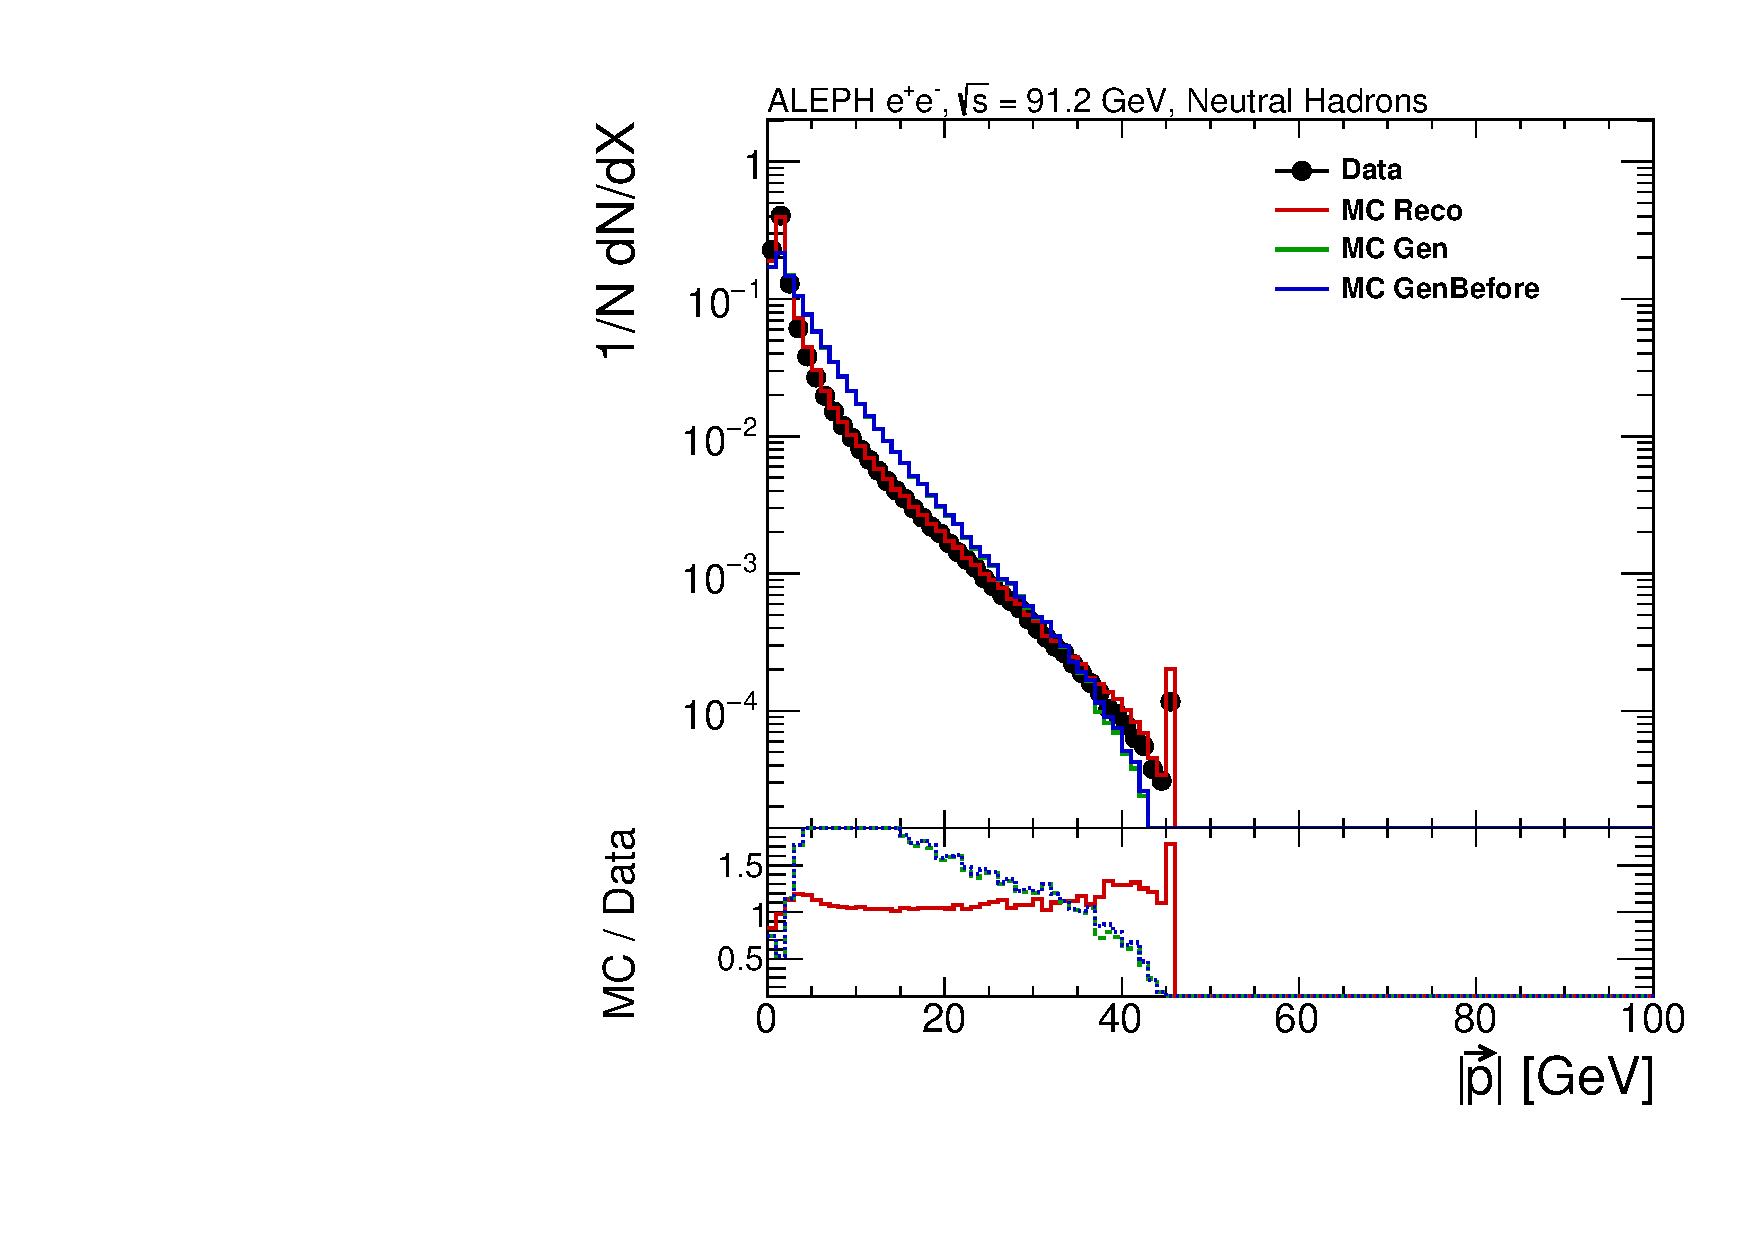
\includegraphics[width=0.325\textwidth]{../Studies/PreliminaryResult/2026-02-17_thrust_iter5/pwflag_kinematics/pwflag5_pmag.pdf}
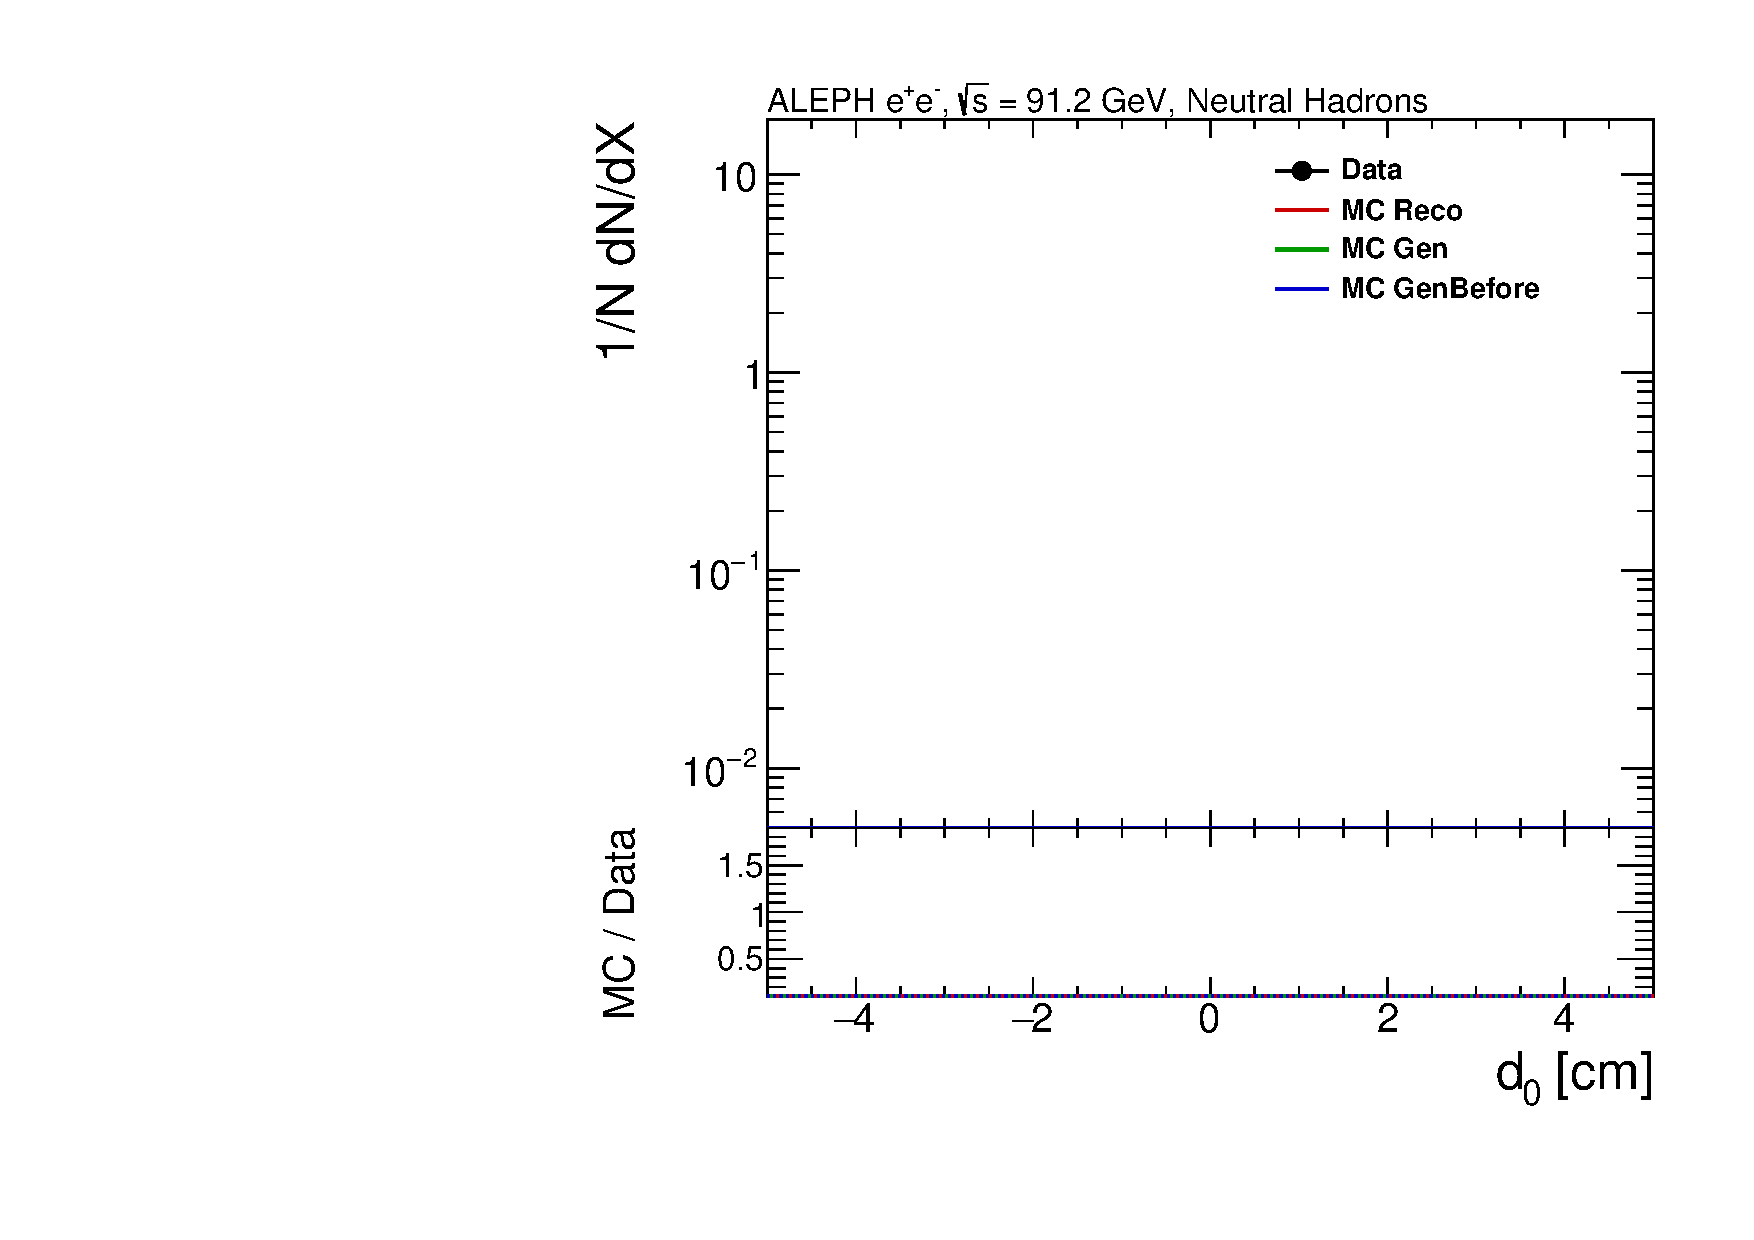
\includegraphics[width=0.325\textwidth]{../Studies/PreliminaryResult/2026-02-17_thrust_iter5/pwflag_kinematics/pwflag5_d0.pdf}
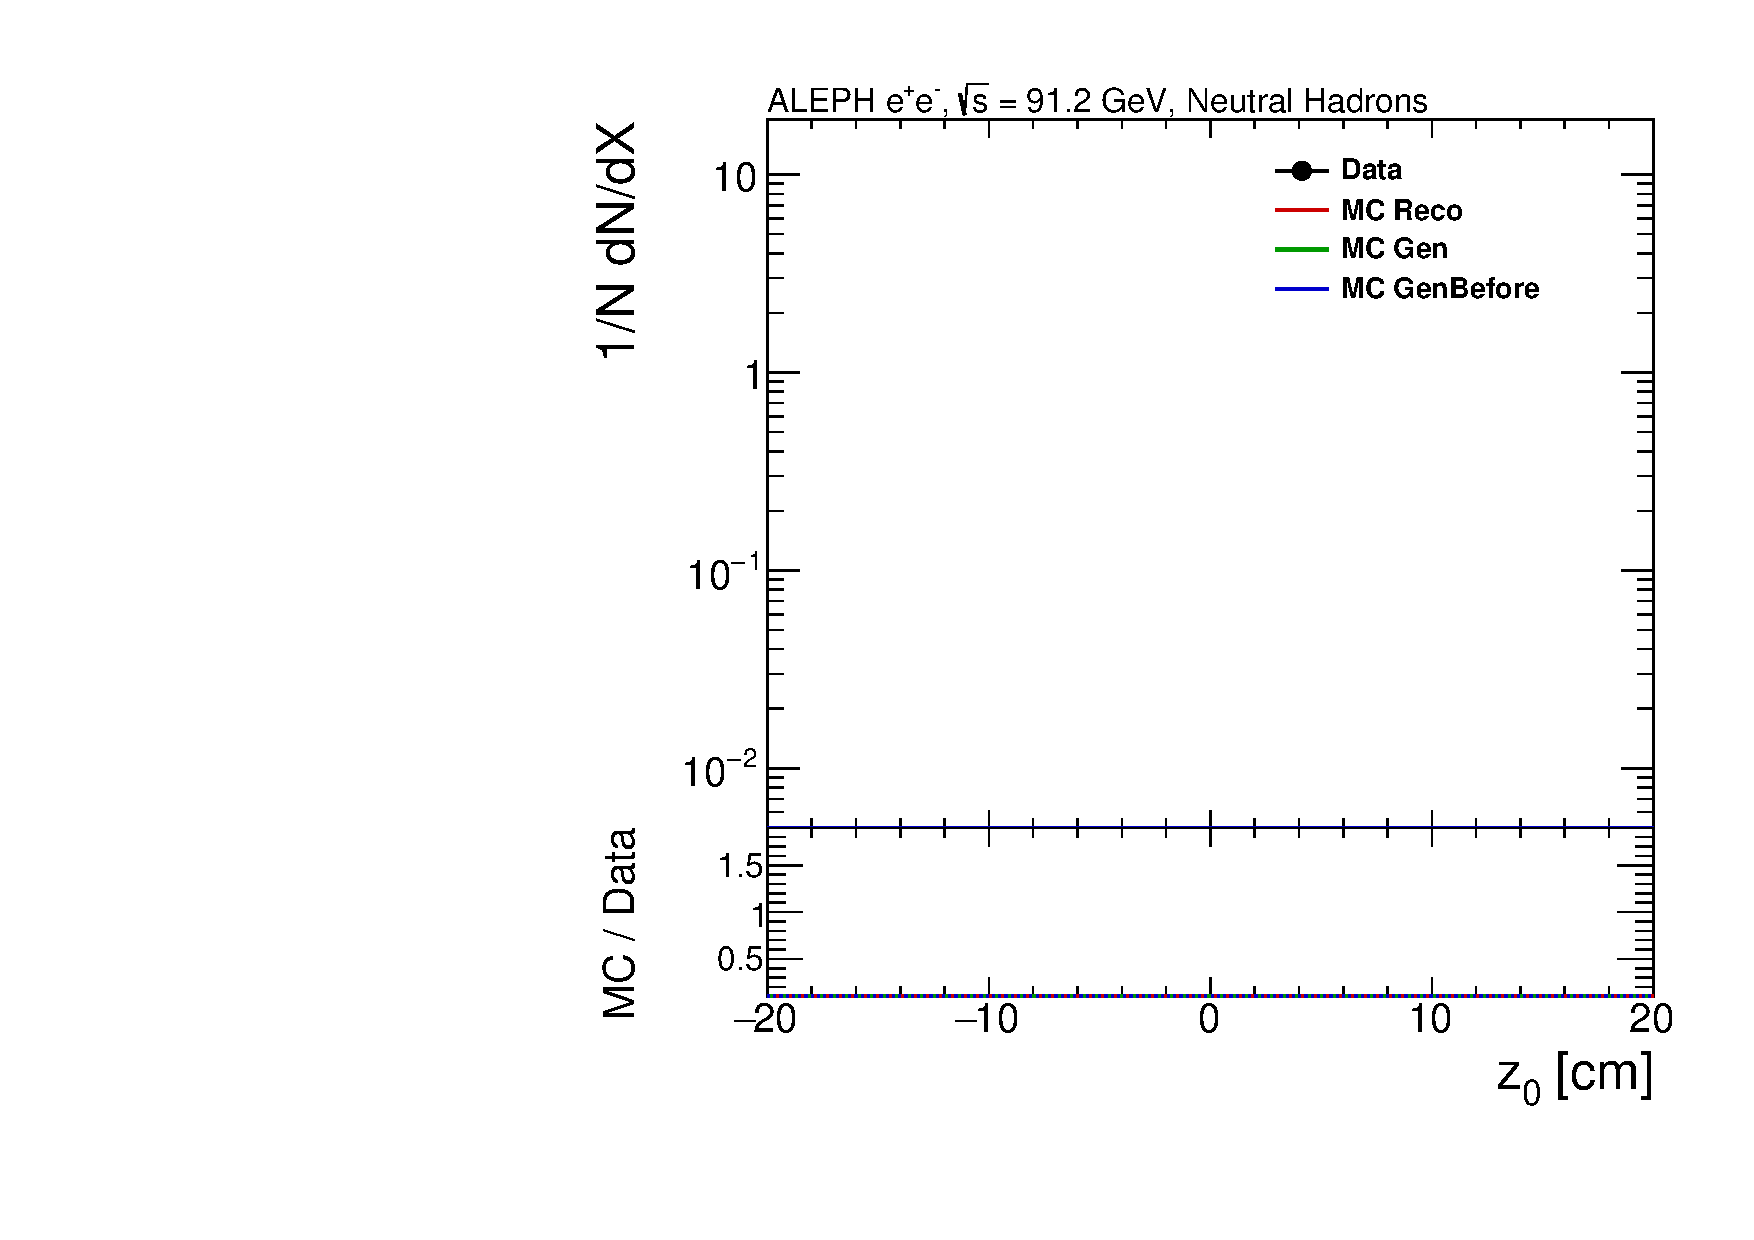
\includegraphics[width=0.325\textwidth]{../Studies/PreliminaryResult/2026-02-17_thrust_iter5/pwflag_kinematics/pwflag5_z0.pdf}
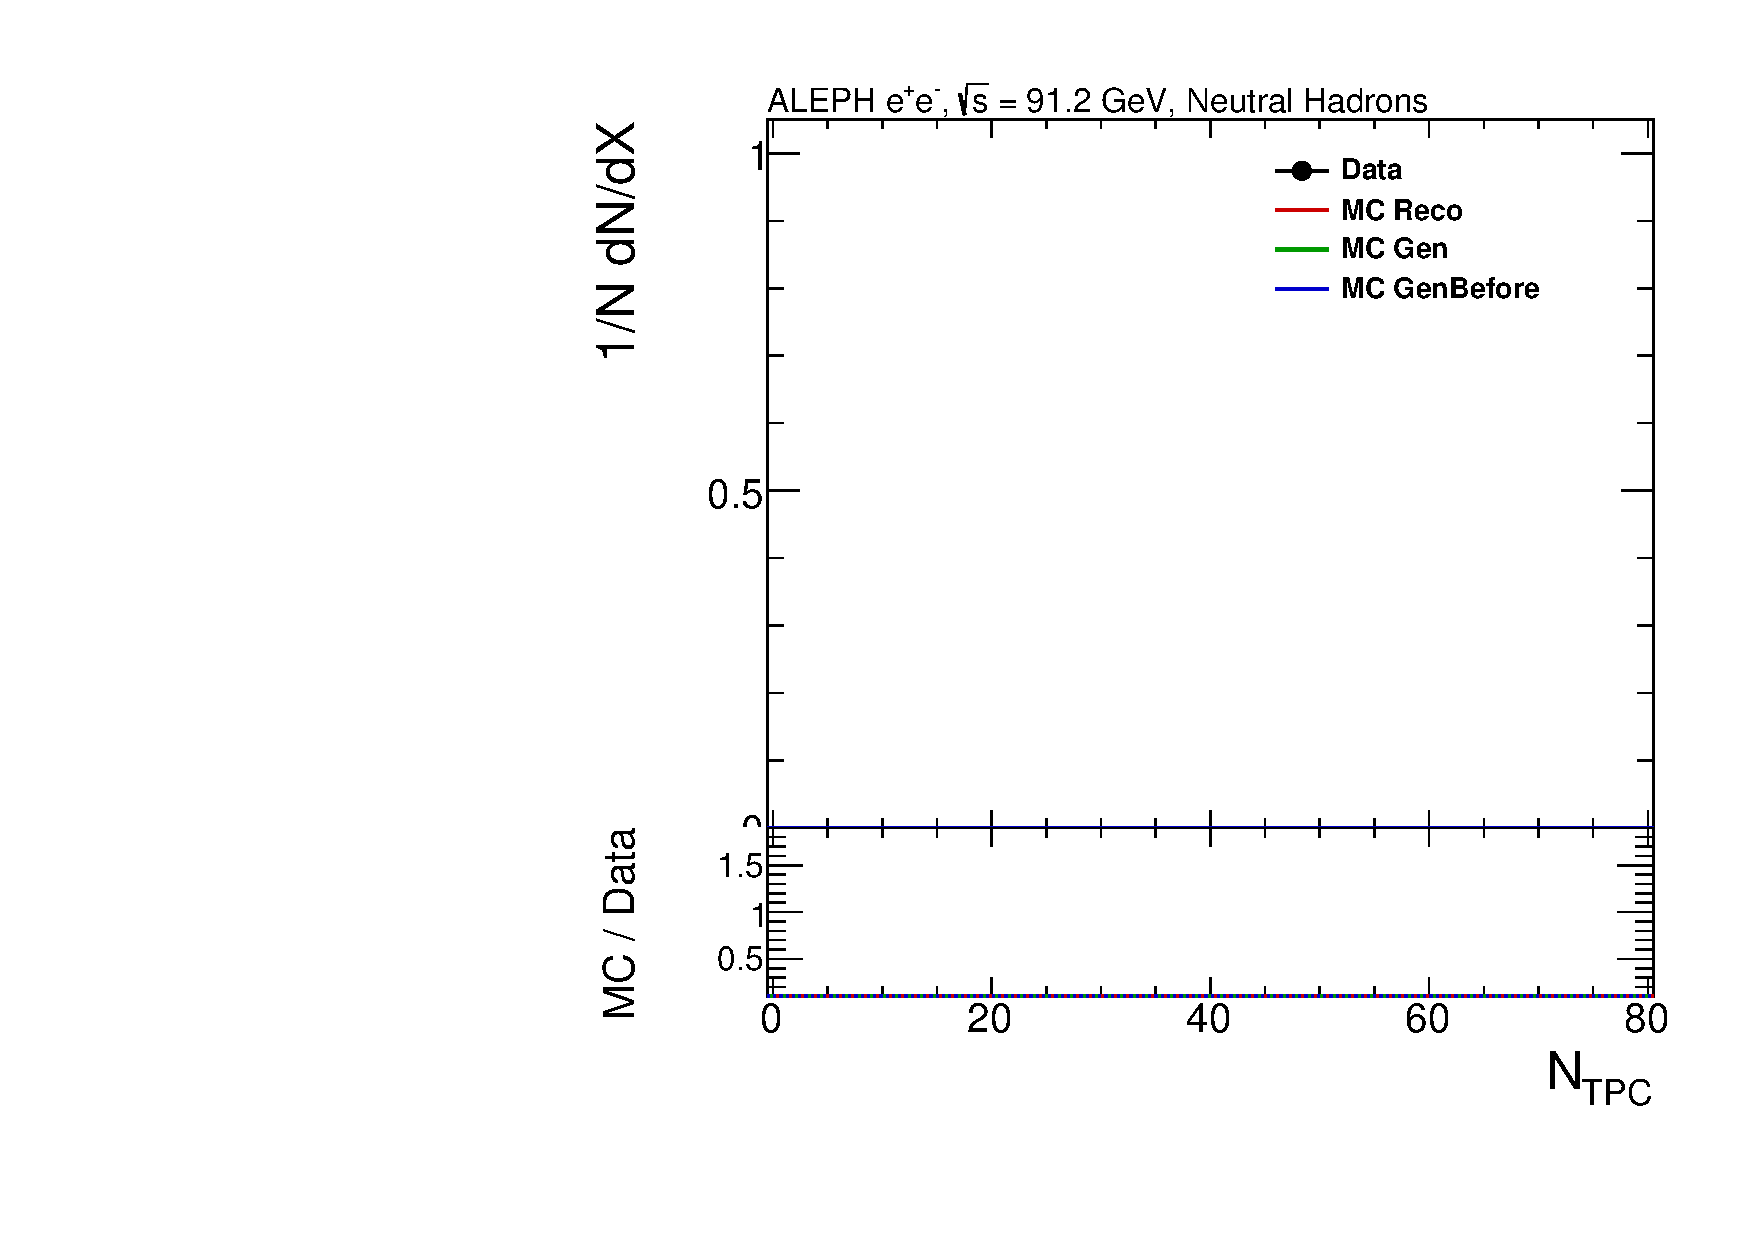
\includegraphics[width=0.325\textwidth]{../Studies/PreliminaryResult/2026-02-17_thrust_iter5/pwflag_kinematics/pwflag5_ntpc.pdf}
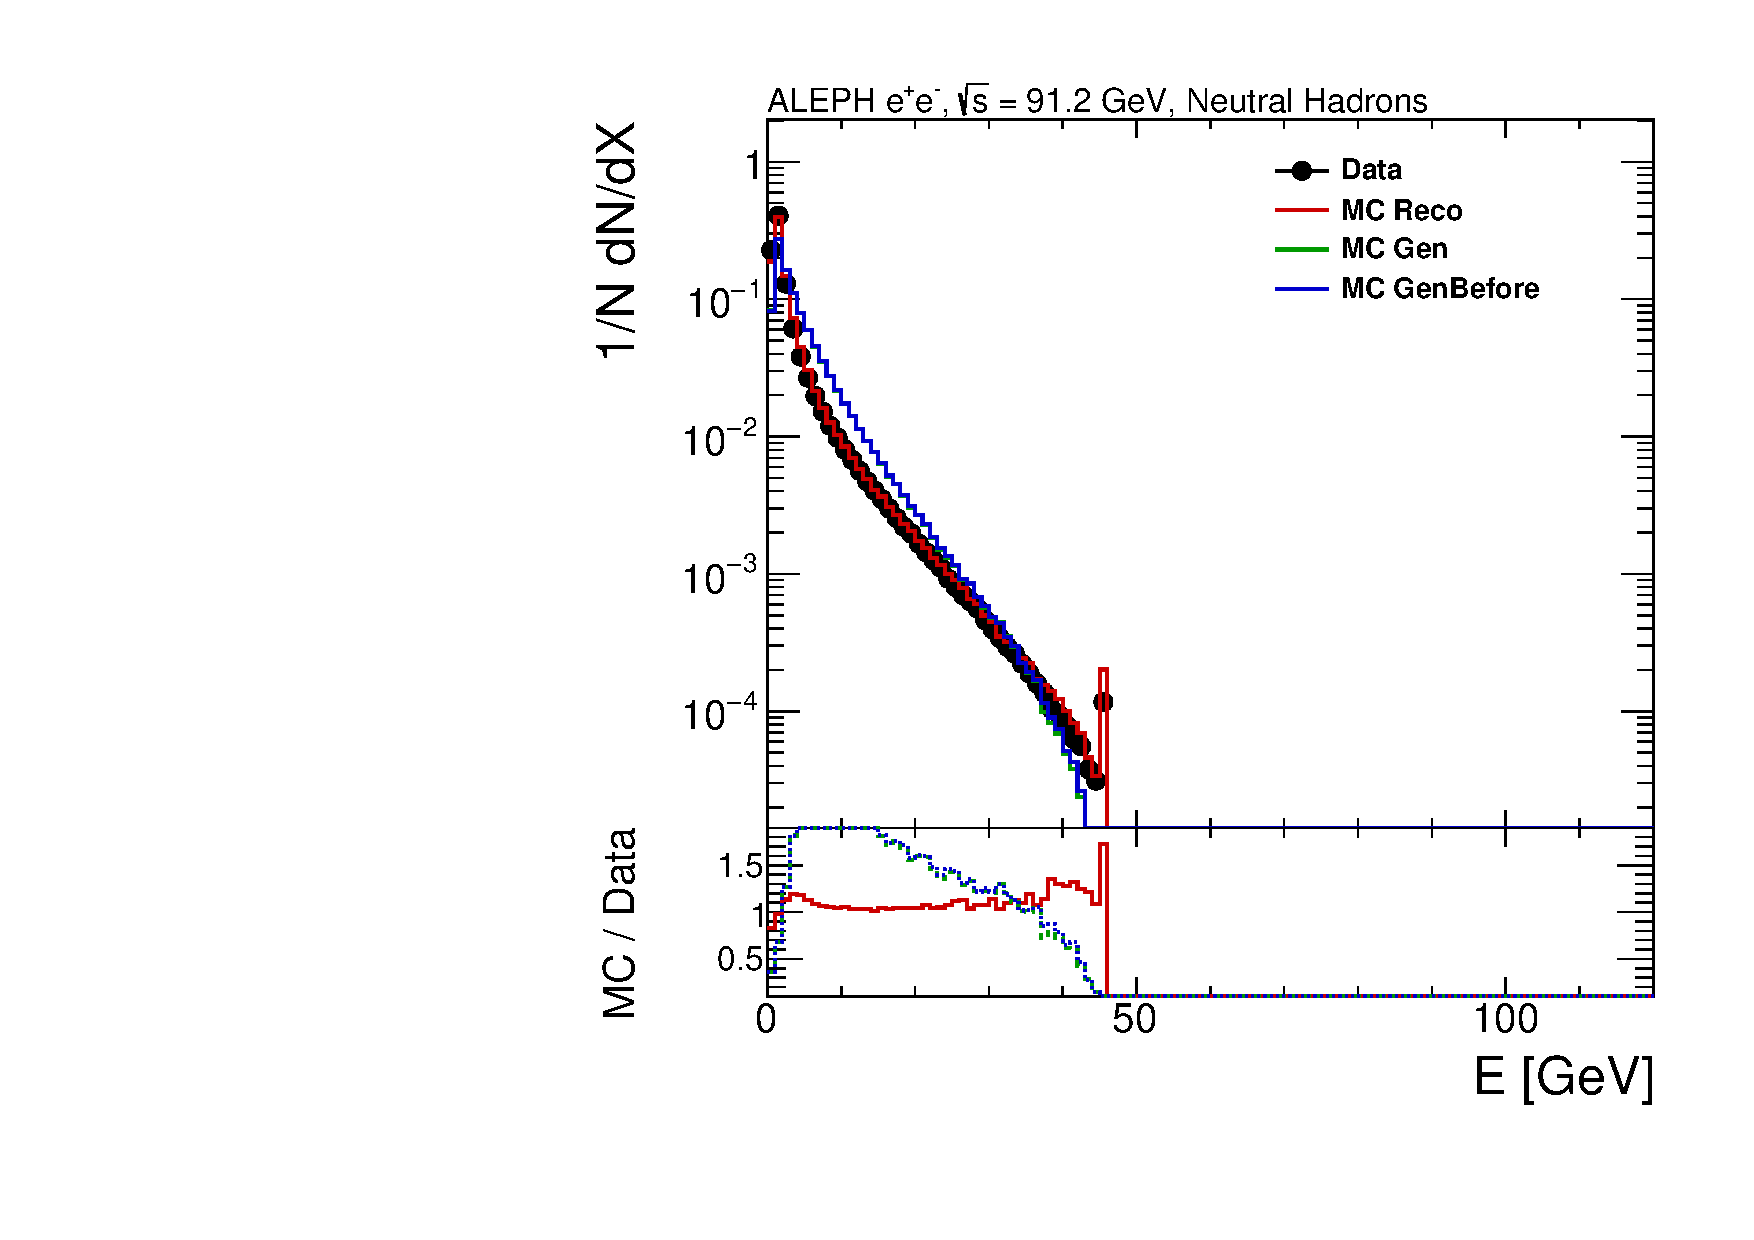
\includegraphics[width=0.325\textwidth]{../Studies/PreliminaryResult/2026-02-17_thrust_iter5/pwflag_kinematics/pwflag5_energy.pdf}
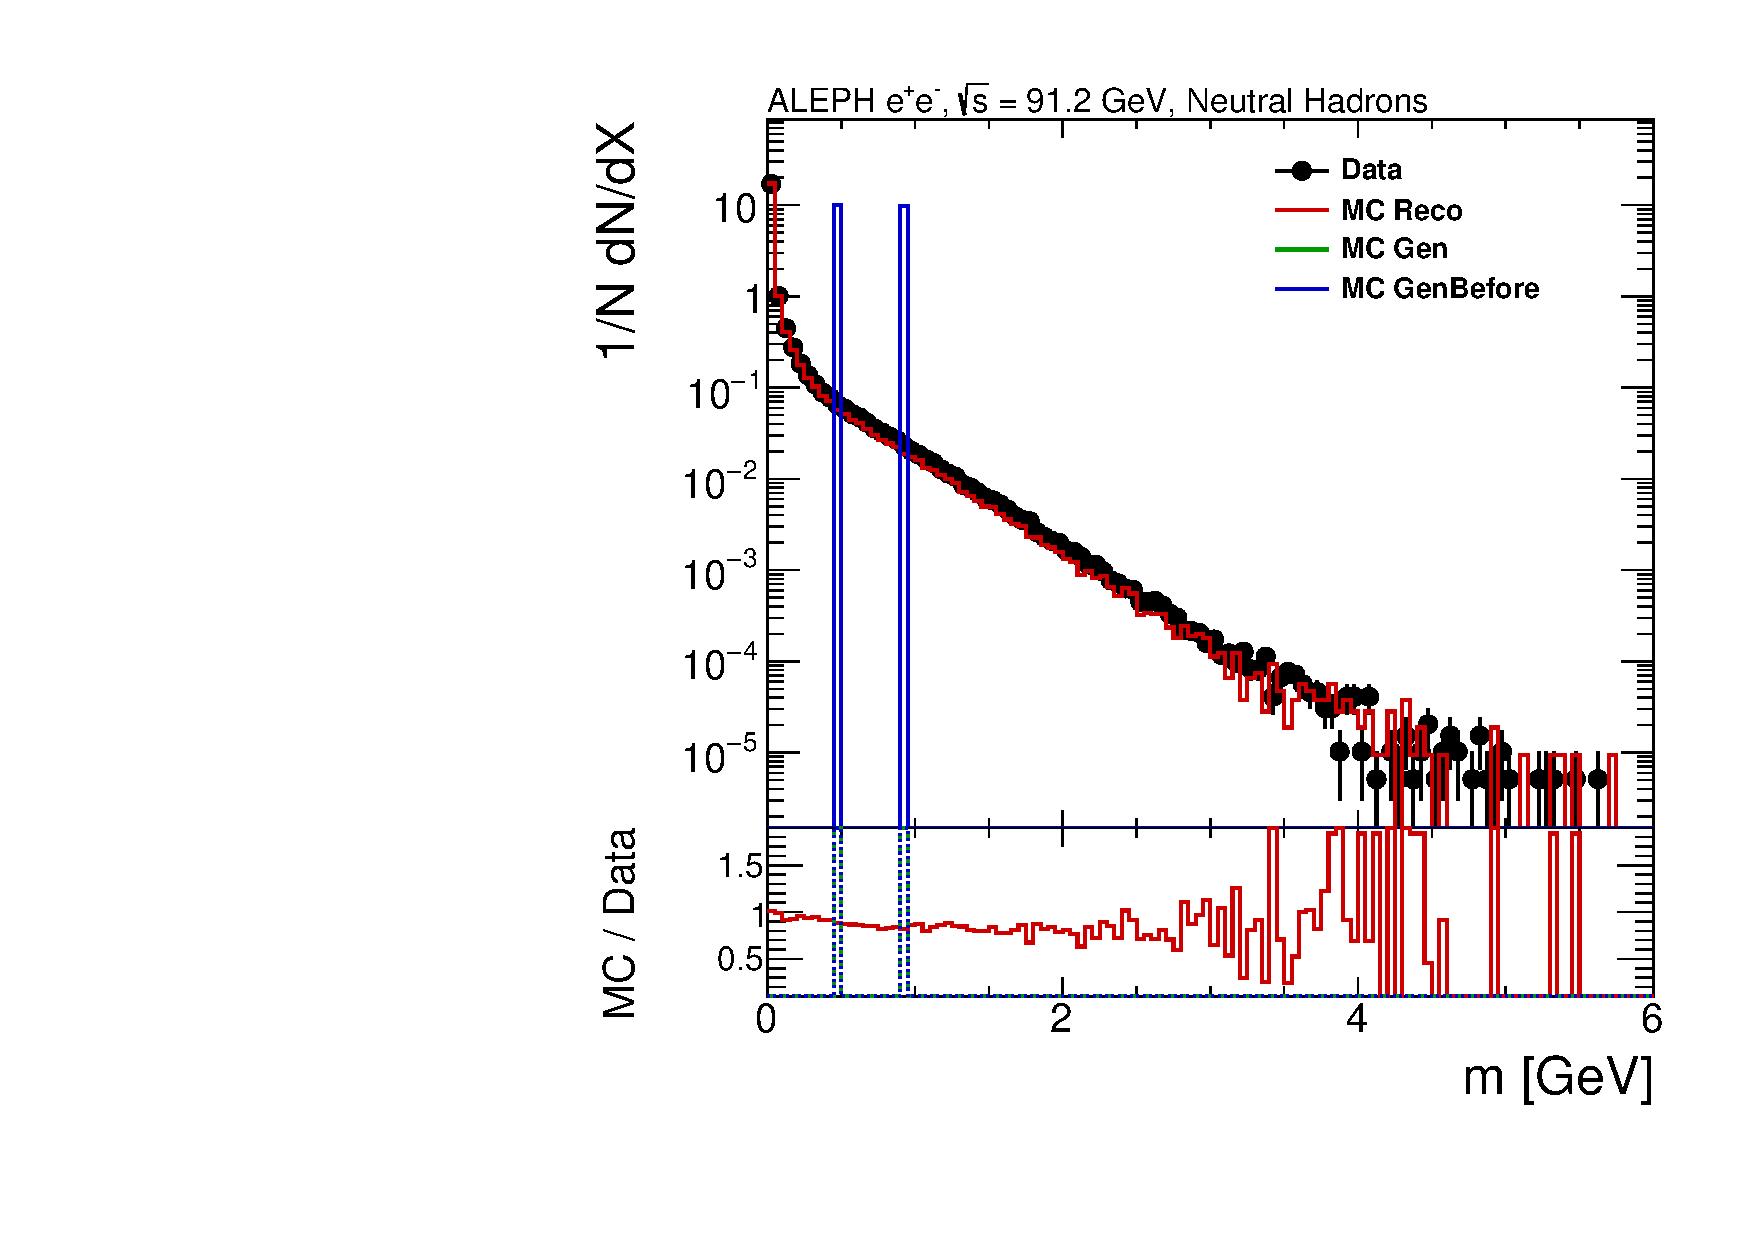
\includegraphics[width=0.325\textwidth]{../Studies/PreliminaryResult/2026-02-17_thrust_iter5/pwflag_kinematics/pwflag5_mass.pdf}
\caption{Complete \texttt{pwflag}=5 kinematic set.}
\label{fig:pwflag5_full}
\end{figure}

\noindent
Figure~\ref{fig:pwflag5_full} completes the neutral-hadron validation; this category is a key
input for neutral-response systematics propagated to the unfolded thrust result. This category is
typically softer and more sensitive to HCAL response and acceptance boundaries, so it is a direct
stress test of the neutral part of the thrust model. The remaining differences in low-statistics
tails are propagated through dedicated neutral-response and cross-check branches in the
experimental systematic program, rather than absorbed into ad hoc selections.


Figure~\ref{fig:pwflag0_full} is the dominant detector-modeling anchor for this analysis because
\texttt{pwflag}=0 tracks provide most of the selected-particle multiplicity and momentum flow. In
this figure, the $\cos\theta$ panel tests geometric acceptance transfer, the impact-parameter
panels test the track-origin and quality region enforced by nominal selections, and the
$N_{\mathrm{TPC}}$ distribution tests detailed tracking response. The $p_T$ and energy spectra are
particularly relevant for thrust because hard tracks can move events across bins near the two-jet
endpoint.

Figures~\ref{fig:pwflag1_full} and~\ref{fig:pwflag2_full} probe the two charged-lepton categories.
Although lower-rate than charged tracks, these objects are important in events with isolated hard
leptons where axis orientation can be sensitive to a small number of particles. Agreement in these
panels demonstrates that category-dependent reconstruction and acceptance do not induce a hidden
bias in thrust inputs.

Figures~\ref{fig:pwflag3_full}--\ref{fig:pwflag5_full} cover $V^0$ candidates, photons, and
neutral hadrons. These categories are essential for total visible energy and hemisphere-sensitive
structure, especially away from the central thrust region. In neutral categories, the angular and
energy spectra are the most important observables because neutral-response mismodeling can directly
alter event-shape normalization and produce larger migration in high-thrust bins. Residual
differences seen in low-statistics tails are propagated via explicit neutral-response systematics
rather than absorbed by additional ad hoc phase-space cuts.

\subsection{Event-level selection observables}

Event-level variables used for hadronic selection are also validated with data/MC comparisons, as shown in Fig.~\ref{fig:event_selection_observables}. These observables summarize the selected particle content and accepted topology that define the phase space used to build detector response and unfolded event-shape spectra.

\begin{figure}[t!]
\centering
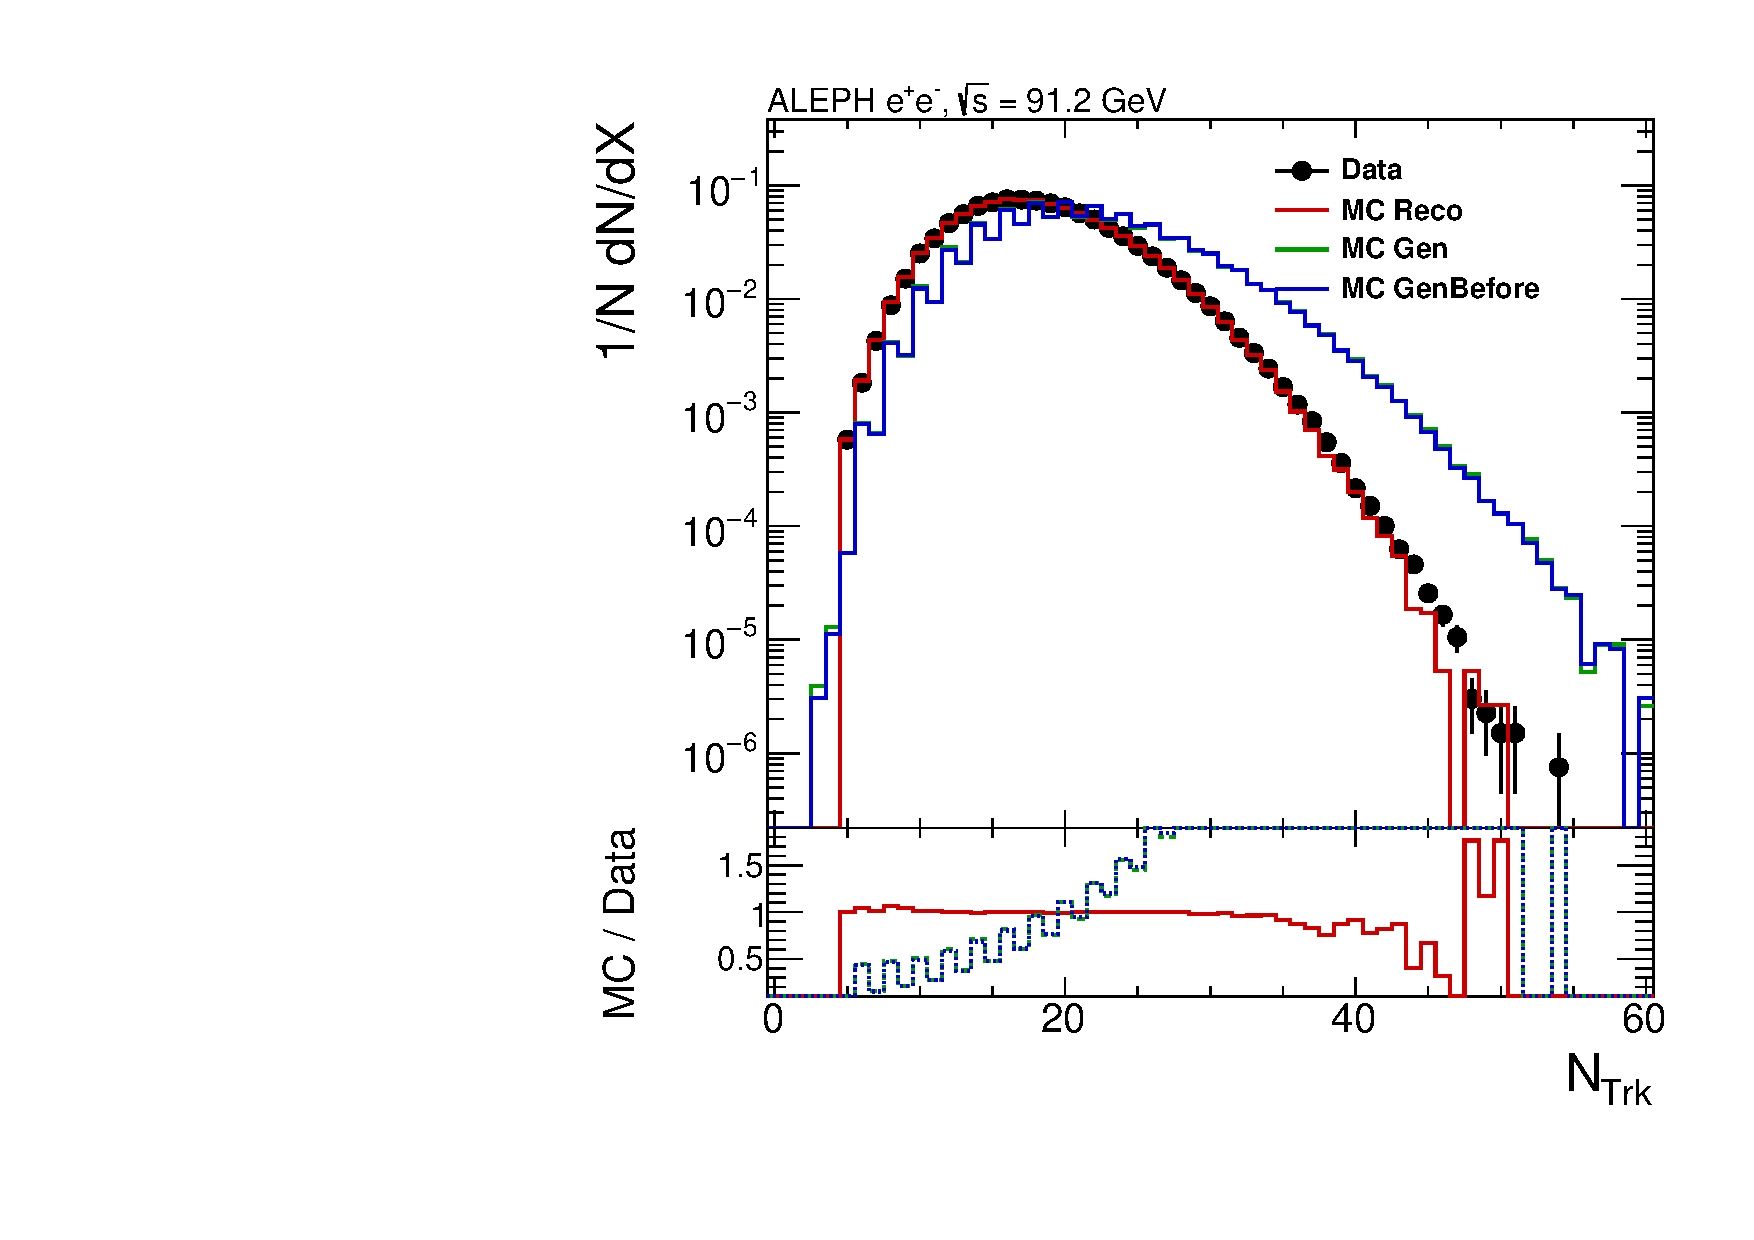
\includegraphics[width=0.495\textwidth]{../Studies/PreliminaryResult/2026-02-17_thrust_iter5/pwflag_kinematics/ntrk.pdf}
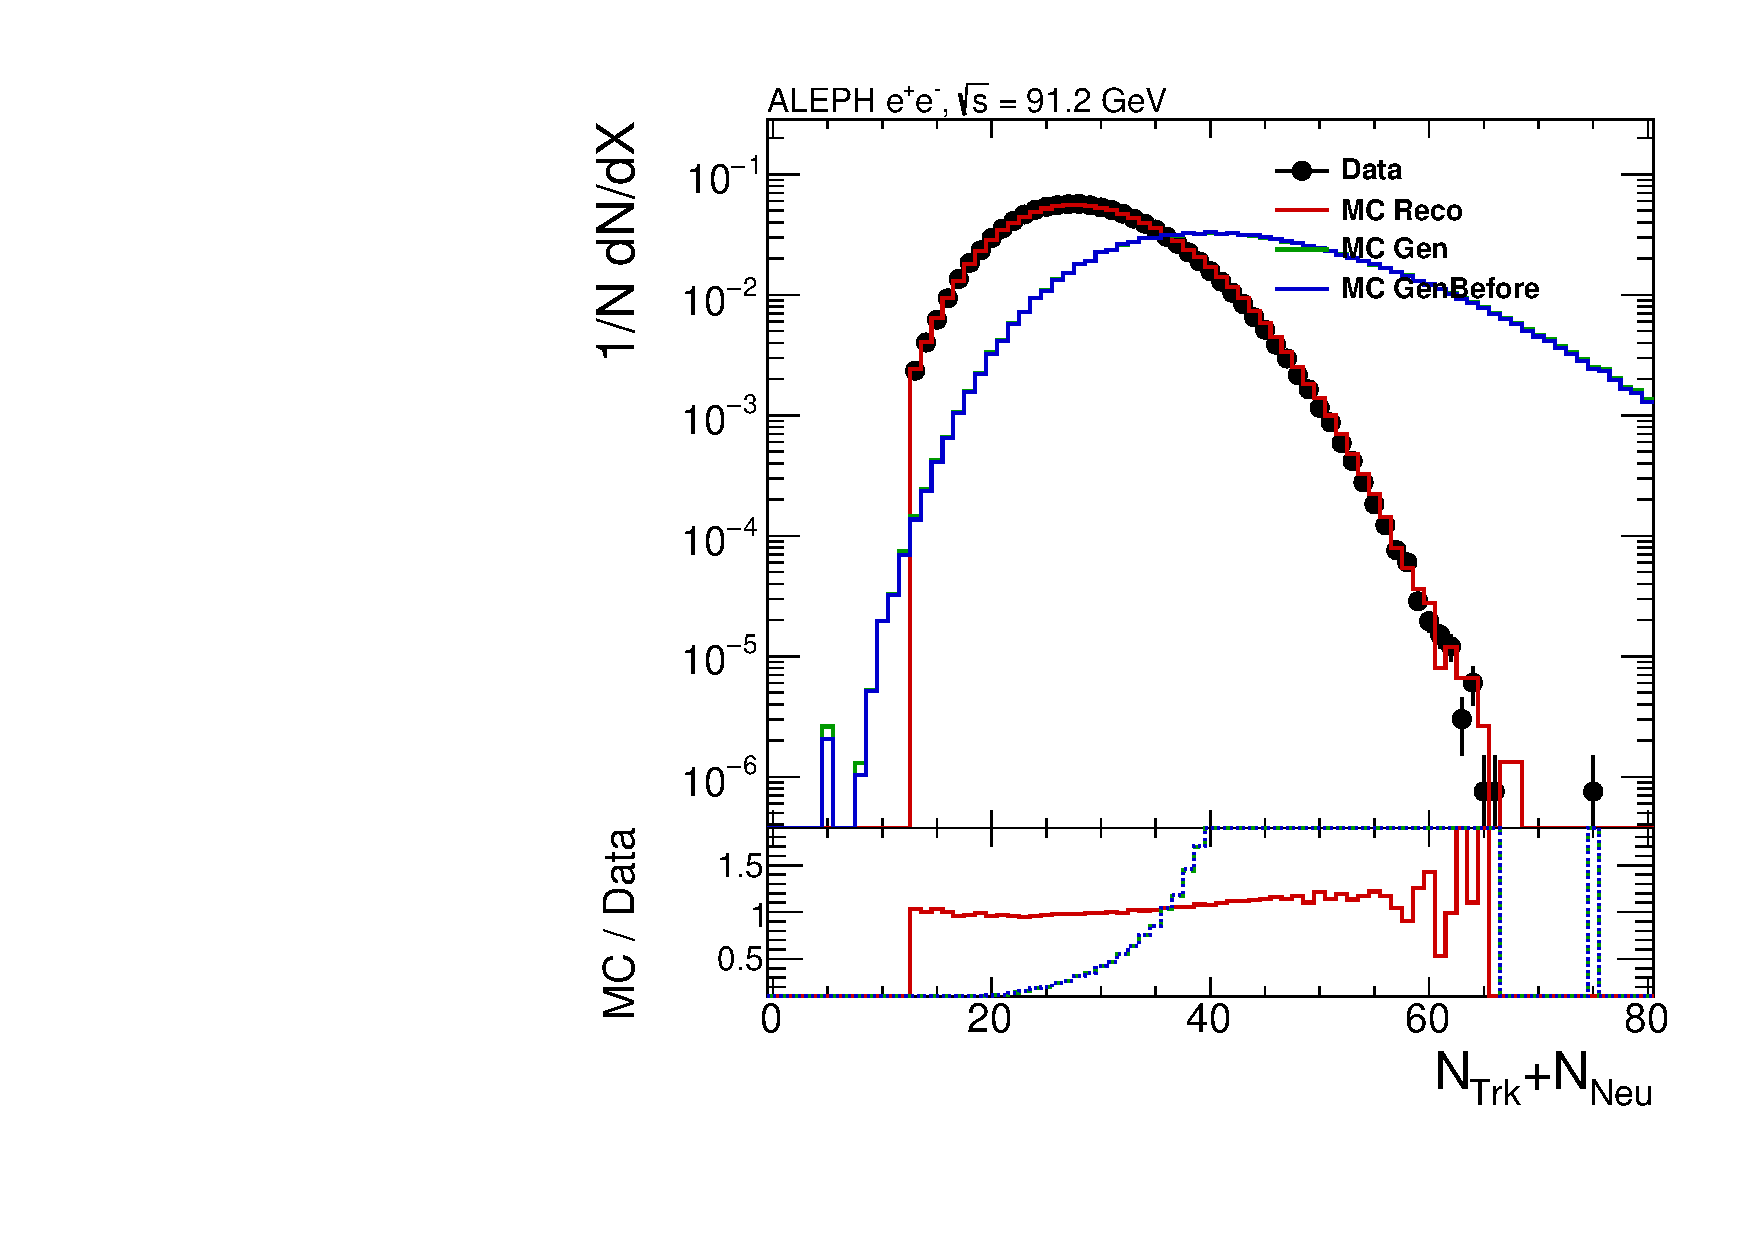
\includegraphics[width=0.495\textwidth]{../Studies/PreliminaryResult/2026-02-17_thrust_iter5/pwflag_kinematics/ntrkPlusNeu.pdf}
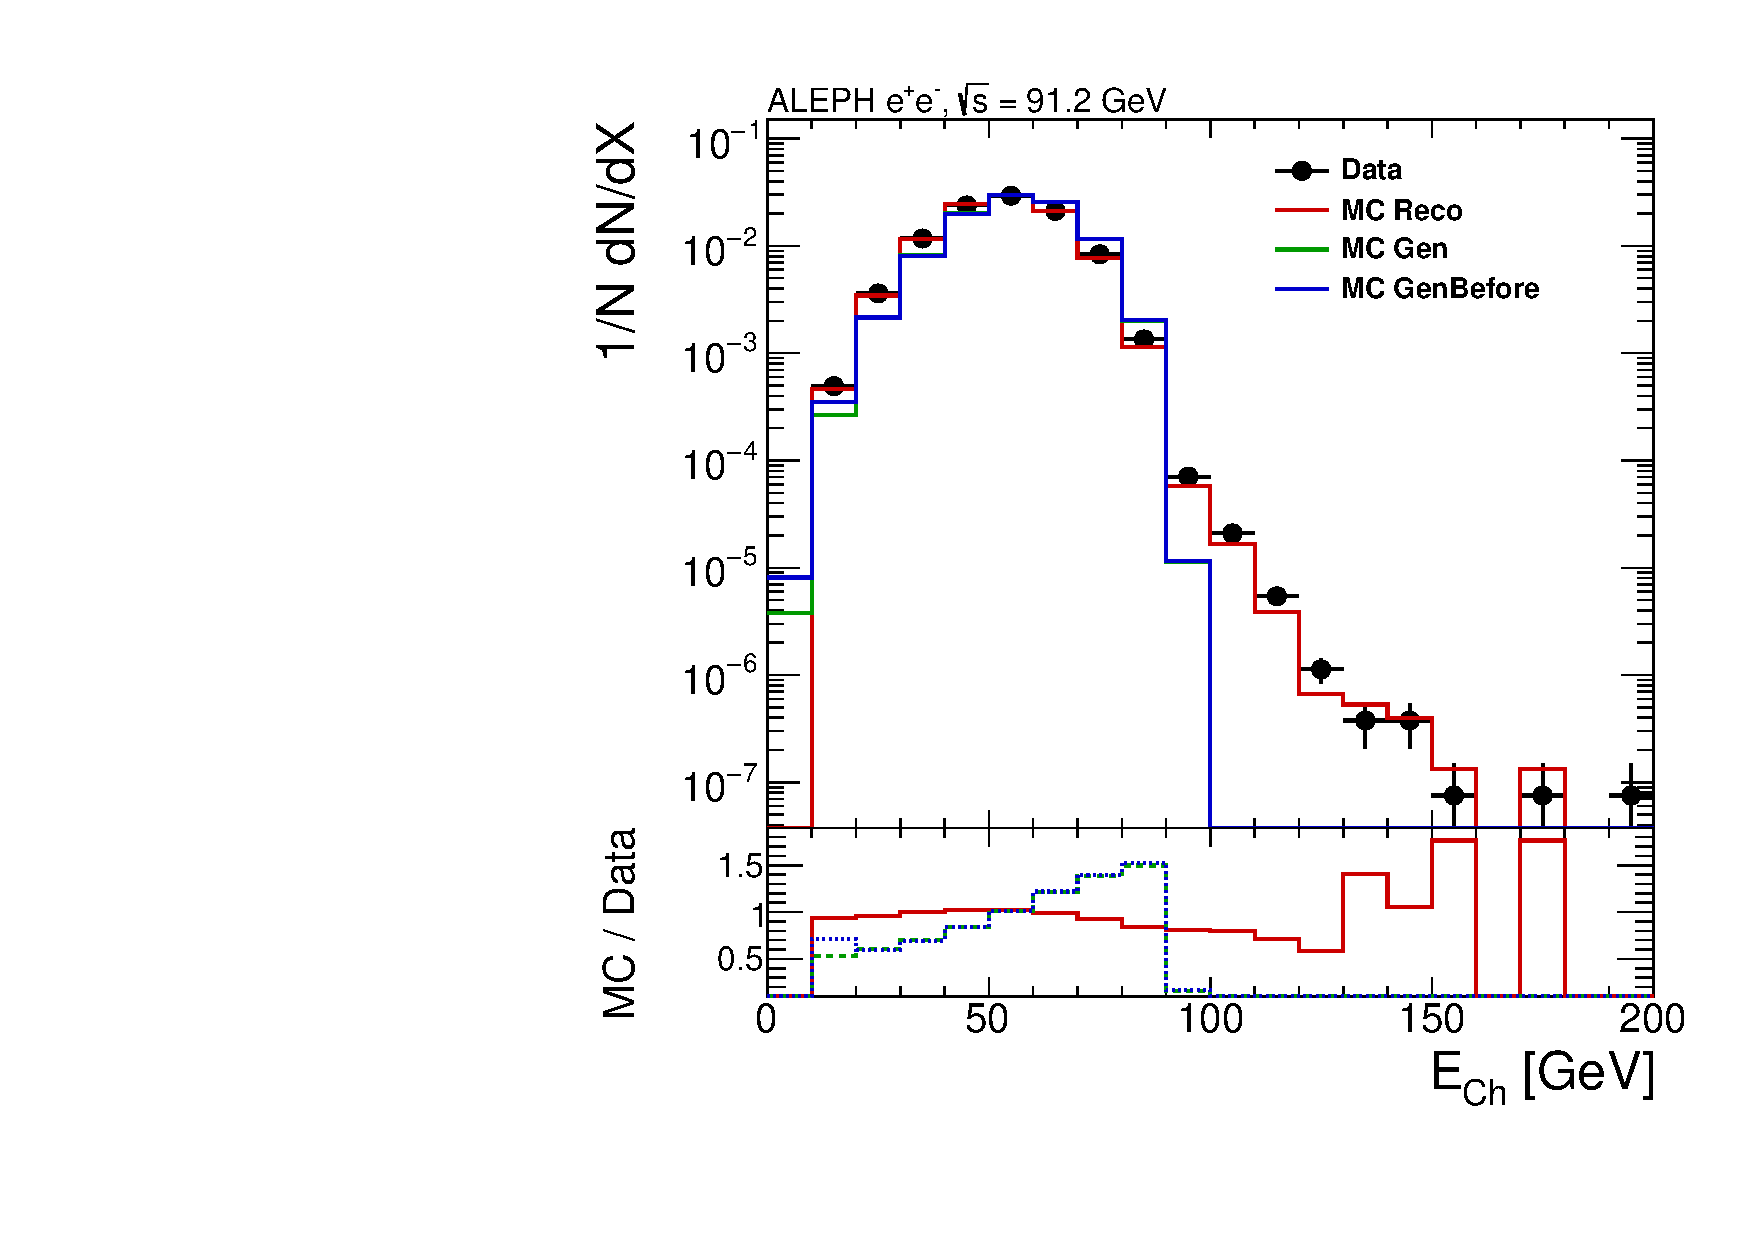
\includegraphics[width=0.495\textwidth]{../Studies/PreliminaryResult/2026-02-17_thrust_iter5/pwflag_kinematics/eCh.pdf}
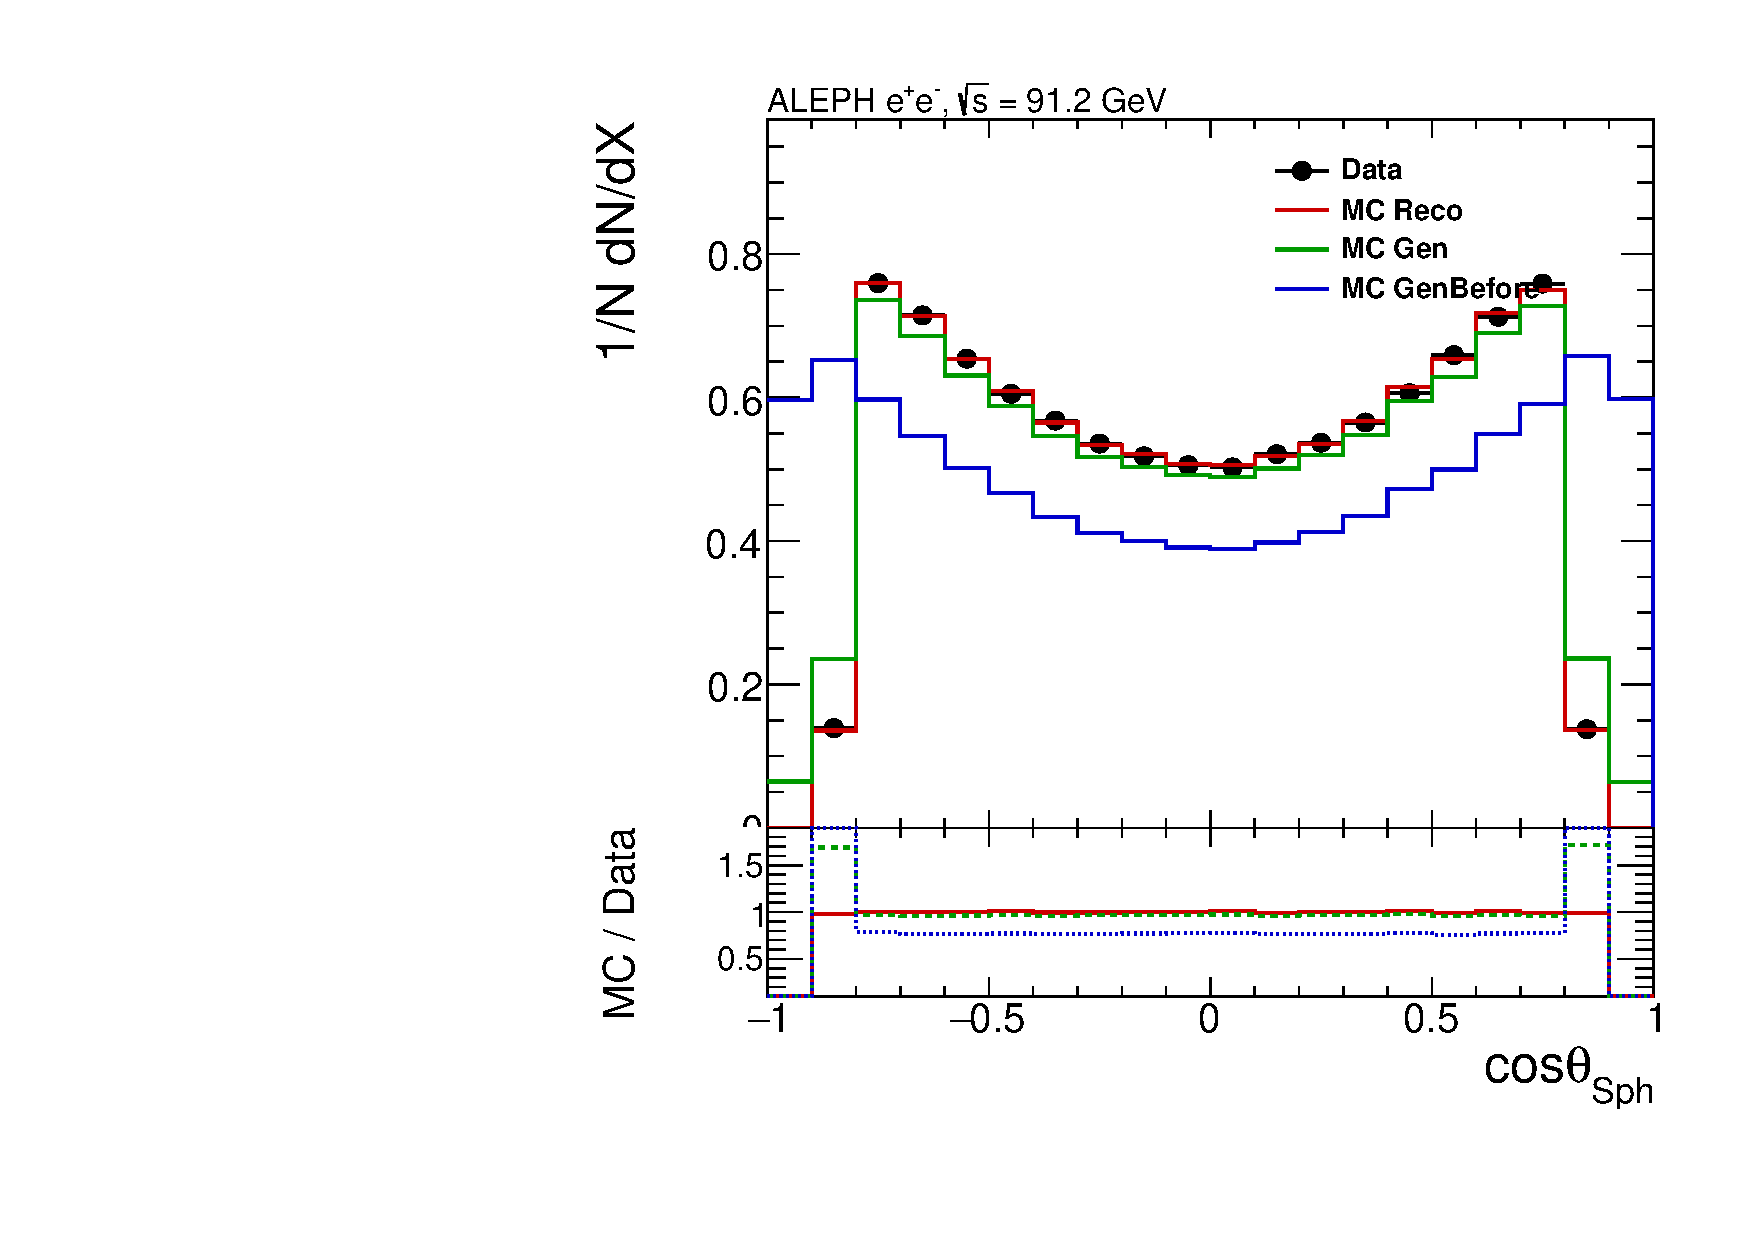
\includegraphics[width=0.495\textwidth]{../Studies/PreliminaryResult/2026-02-17_thrust_iter5/pwflag_kinematics/cosThetaSph.pdf}
\caption{Event-level observables used in the nominal hadronic selection; legends include detector-level data/MC and generator-level references.}
\label{fig:event_selection_observables}
\end{figure}

The event-level panels close the logic between object-level selections and the final sample
entering event-shape reconstruction. $N_{\mathrm{trk}}$ and
$N_{\mathrm{trk}}+N_{\mathrm{neu}}$ test whether multiplicity thresholds sculpt data and MC in a
consistent way; this is critical because those same multiplicities enter hadronic-event
preselection and determine which events contribute to response filling. $E_{\mathrm{Ch}}$ checks
charged-energy modeling near the hadronic-selection boundary at 15 GeV, and
$\cos\theta_{\mathrm{Sph}}$ tests whether accepted event topology is similarly contained in
detector acceptance for data and MC.

Overall agreement in the high-statistics regions supports the response-model baseline used for IBU.
The visible differences are concentrated in lower-populated tails and near selection boundaries,
where statistical fluctuations and detector-response limitations are expected to be larger. These
regions are not ignored: their impact is propagated through the experimental systematic program and
is reflected in the final uncertainty decomposition.

\FloatBarrier
\clearpage

\section{Analysis method}
\label{sec:method}

This section documents the thrust analysis method, including the observable
definition, the response construction, the unfolding setup, systematic execution,
and the correction and covariance workflow. Executable workflow details, command
sequences, and pseudocode are collected in
Appendix~\ref{sec:app_workflow_code} to keep the main text focused on physics.

\subsection{Observable definition and nominal configuration}

The thrust observable is defined as~\cite{PhysRevLett.39.1587}
\begin{equation}
T = \max_{\hat{n}} \frac{\sum_i |\vec{p}_i \cdot \hat{n}|}{\sum_i |\vec{p}_i|},
\end{equation}
with all selected charged and neutral reconstructed objects from Sec.~\ref{sec:event_selection} entering the sum.
We first adopt bins identical to the published ALEPH event-shape analysis~\cite{Heister:2003aj}, using 50 uniform bins over $0.5 \le T < 1.0$ (bin width $\Delta T = 0.01$), which enables a direct bin-by-bin comparison with the published ALEPH result. We then test fine bins throughout the full thrust space to assess the usable binning resolution in different regions, particularly in the high-thrust (low $\tau = 1-T$) regime. The thrust resolution study in Sec.~\ref{sec:thrust_resolution} informs the finest binning achievable in each region.

\begin{table}[t!]
\centering
\begin{tabularx}{0.98\textwidth}{p{0.33\textwidth} X}
\hline
Item & Nominal configuration \\
\hline
Observable & Thrust $T$ \\
Range & $0.5 \le T < 1.0$ \\
Binning & 50 uniform bins \\
Reco/gen matching key & \texttt{uniqueID} \\
Reco selection branch & \texttt{passEventSelection} \\
Nominal IBU iterations & 5 \\
Hadronic correction & enabled ($N_{\mathrm{genBefore}}/N_{\mathrm{gen}}$) \\
Statistical covariance input & unfolding covariance transformed to normalized differential-thrust basis \\
RooUnfold covariance method & \texttt{kCovariance} (analytical error propagation) \\
Particle-level target & stable hadrons ($c\tau > 10$~mm), inclusive over full hadronic Z phase space \\
\hline
\end{tabularx}
\caption{Nominal analysis configuration used in the thrust Iterative Bayesian Unfolding workflow.}
\label{tab:method_config}
\end{table}


The nominal run uses $N_{\mathrm{iter}}=5$ and applies the post-unfolding hadronic event correction from
\texttt{tgenBefore/tgen}.
The nominal branch is the only run with covariance enabled; variation branches are propagated through signed shifts relative to the nominal spectrum.

\subsection{Response construction from matched MC}

Response filling uses event-by-event matching through \texttt{uniqueID}. Reconstructed MC entries with
\texttt{passEventSelection} equal to 1 define the selected detector-level phase space. Generator-level entries are then matched to this selected set and used to fill:
\begin{itemize}
\item the response counts matrix;
\item the miss term required by RooUnfold for inefficiency handling.
\end{itemize}

This matched-response construction enforces a consistent phase-space definition between detector-level selection and generator-level truth used in unfolding. Generator-level events with no matched reco entry (misses, from reconstruction inefficiency or acceptance gaps) are handled by RooUnfold's efficiency correction. Reco-level events with no matched gen entry (fakes, from beam background or random coincidences) are not expected to be significant in the archived ALEPH hadronic sample and are not separately subtracted.

\subsection{Iterative Bayesian Unfolding setup and iteration choice}

Detector correction is performed with RooUnfold Bayesian unfolding,
\begin{equation}
U_j^{(n+1)} = \frac{1}{\epsilon_j}\sum_i M_i\,\frac{R_{ij}\,\pi_j^{(n)}}{\sum_k R_{ik}\,\pi_k^{(n)}},
\end{equation}
where $M_i$ is the measured detector-level spectrum, $R_{ij}$ is the response, and $\pi_j^{(n)}$ is the iteration prior.

The prior for the first iteration is taken as the generator-level MC truth distribution $\pi_j^{(0)} = N_{\mathrm{gen}}(j)$, the standard RooUnfold default. This choice initializes the unfolding close to the expected truth shape and avoids any flat-prior amplification of high-frequency fluctuations in the first iteration.

The nominal regularization is
\begin{equation}
N_{\mathrm{iter}}=5,
\end{equation}
with $N_{\mathrm{iter}}=4$ and $6$ propagated as unfolding-regularization systematic branches.
The iteration-choice diagnostics are shown in
Figs.~\ref{fig:refold_selected_iters} and~\ref{fig:iteration_choice_diagnostics}, including $N=4,5,6,10,100$ refolding checks.

The response matrix has a diagonal fraction of $f_{\mathrm{diag}}=0.33$, meaning approximately two-thirds of events migrate out of their generated thrust bin at reconstruction level. This level of bin-to-bin migration is expected for thrust at ALEPH given the finite charged-particle momentum resolution and the sensitivity of thrust to soft particles near the event boundary. It implies that the unfolding correction is non-trivial and that the choice of regularization strength meaningfully affects the result. The iteration diagnostics in Fig.~\ref{fig:iteration_choice_diagnostics} show that the closure-shape $\chi^2/\mathrm{ndf}$ is stable and the iteration-to-iteration change in the unfolded spectrum is small for $N_{\mathrm{iter}} \in \{4,5,6\}$, providing confidence that $N_{\mathrm{iter}}=5$ sits in a well-regularized plateau rather than near an instability. The propagated $N_{\mathrm{iter}}=4,6$ systematic covers residual regularization-bias uncertainty at the level documented in Sec.~\ref{sec:systematics}.

The ``miss'' term---generator-level events with no matched reconstructed counterpart---is
documented in Fig.~\ref{fig:miss_term_efficiency}. These are events that fail the
reco-level hadronic event selection despite being generated within the fiducial volume.
The miss rate is concentrated at low thrust ($T\lesssim0.7$) and in events with low
charged multiplicity, consistent with the hadronic event selection removing poorly
reconstructed events. RooUnfold accounts for miss events via
\texttt{response.Miss($x_{\mathrm{gen}}$)}, which correct the unfolded spectrum for
this acceptance effect.

\begin{figure}[t!]
\centering
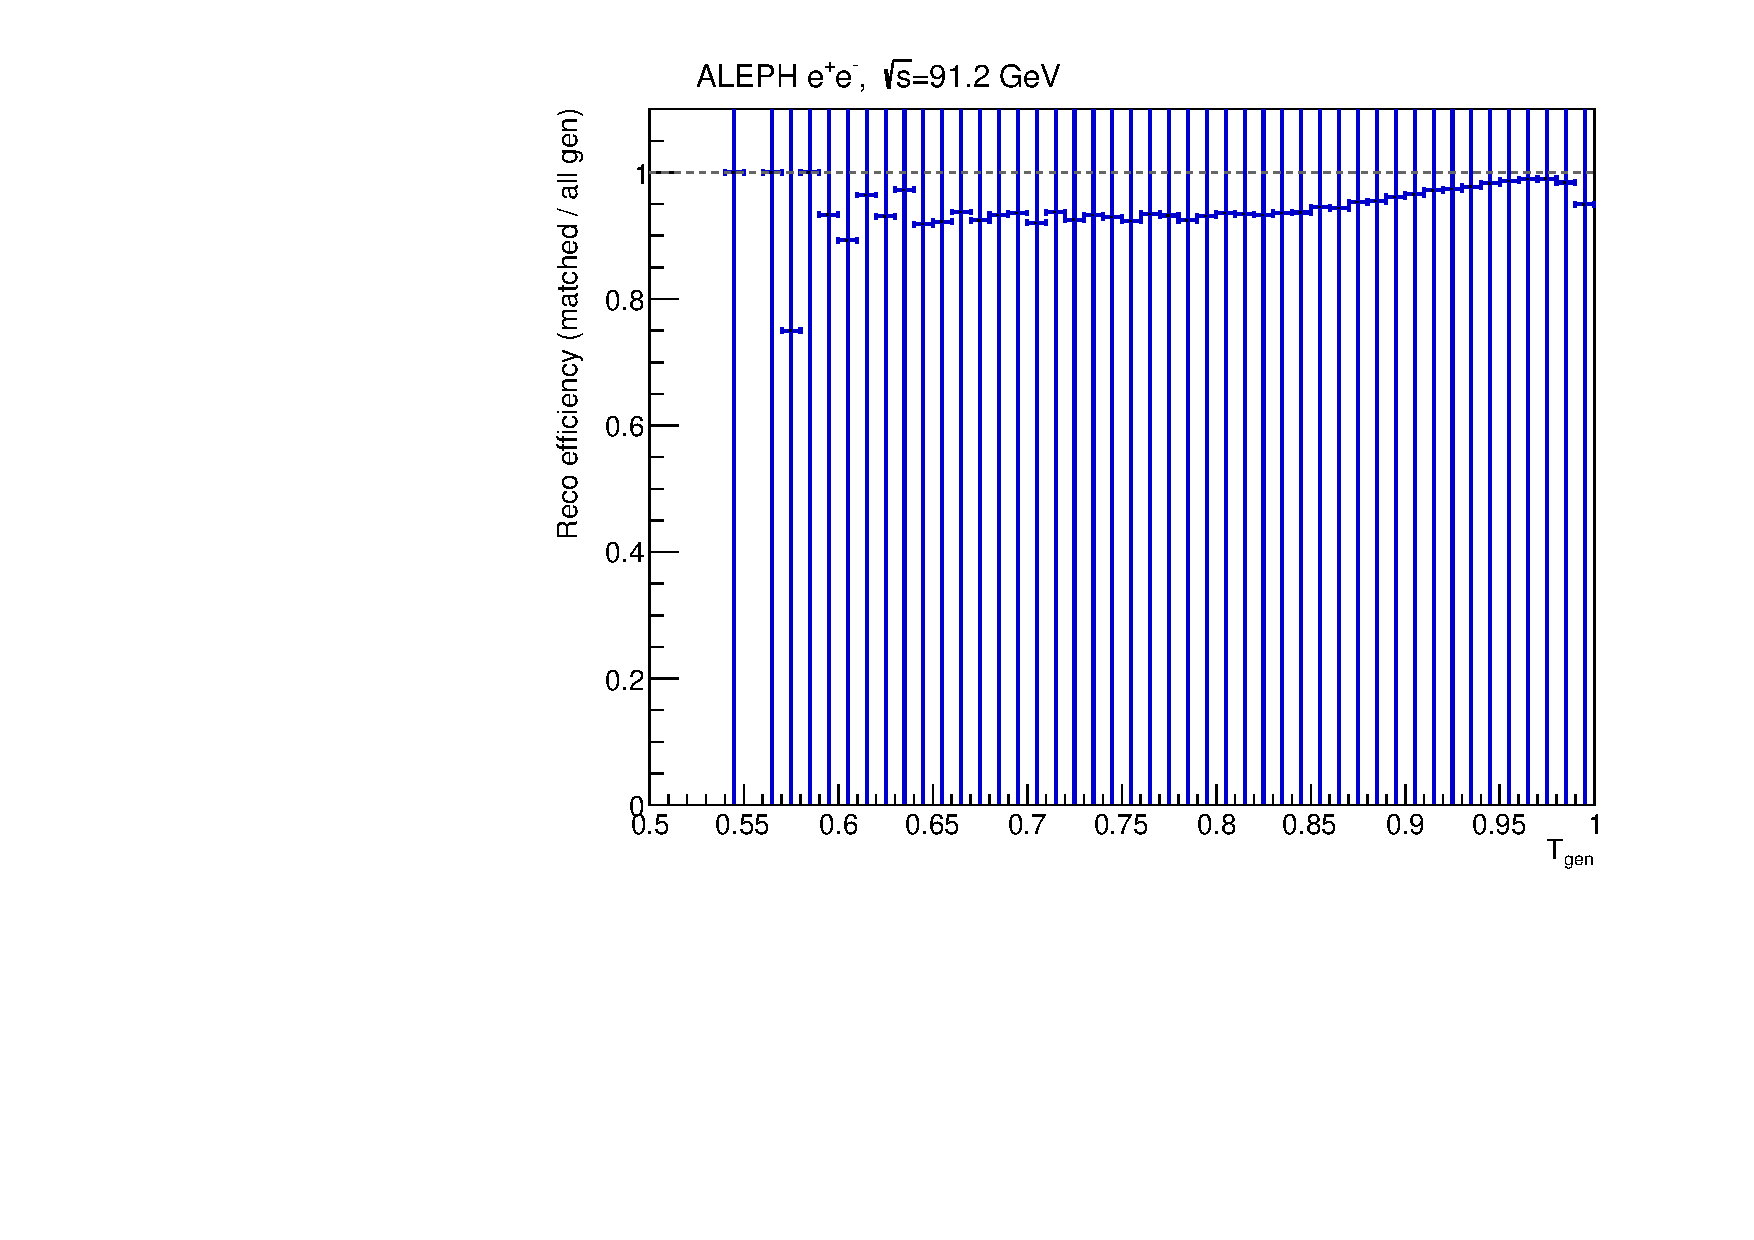
\includegraphics[width=0.49\textwidth]{../Studies/Phase2_Checks_2026-03-03/plots/miss_term/miss_term_efficiency.pdf}
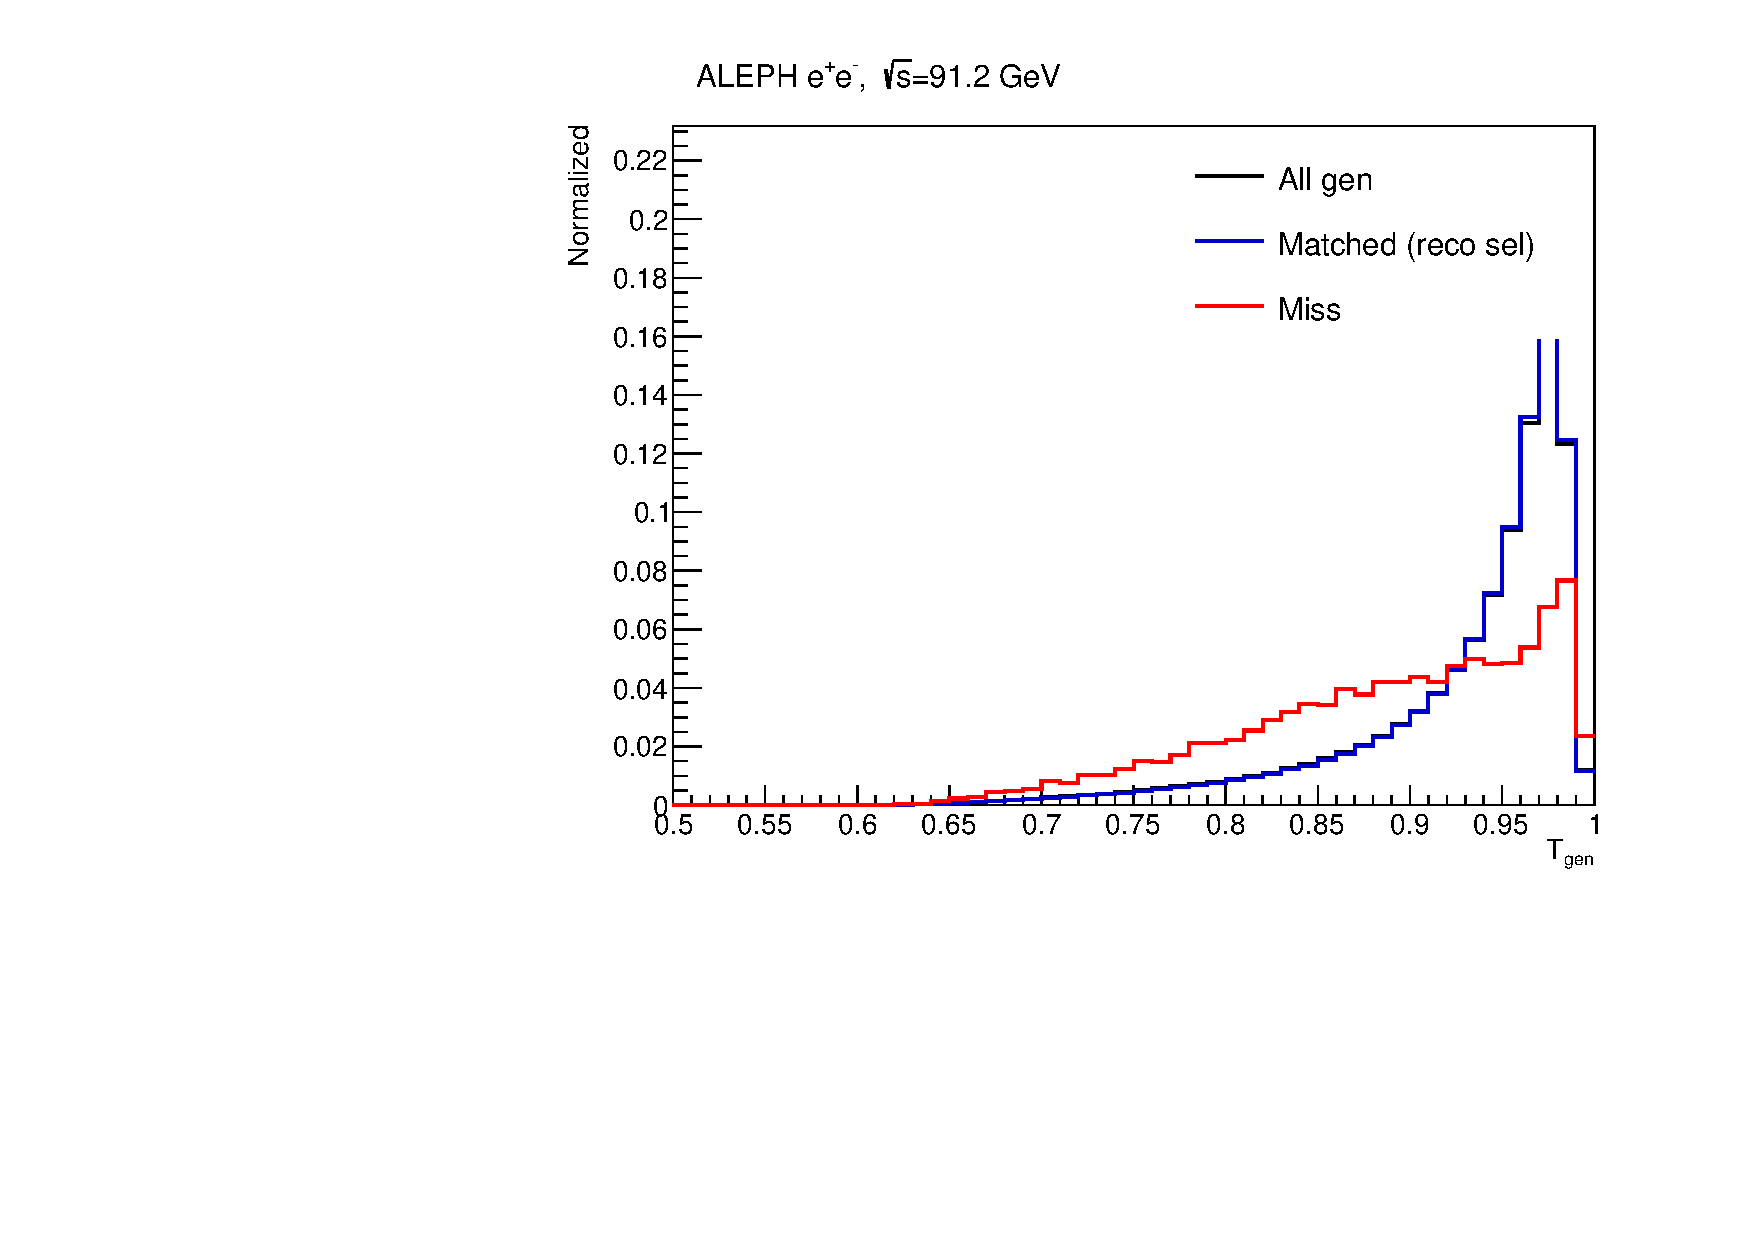
\includegraphics[width=0.49\textwidth]{../Studies/Phase2_Checks_2026-03-03/plots/miss_term/miss_term_thrust.pdf}
\caption{Left: reco efficiency (matched/all gen) as a function of $T_{\mathrm{gen}}$.
Right: thrust distributions for all gen, matched, and miss events (normalized to unit area).
Miss events are concentrated at low thrust and low multiplicity, consistent with
events failing the hadronic event selection.}
\label{fig:miss_term_efficiency}
\end{figure}

\begin{figure}[t!]
\centering
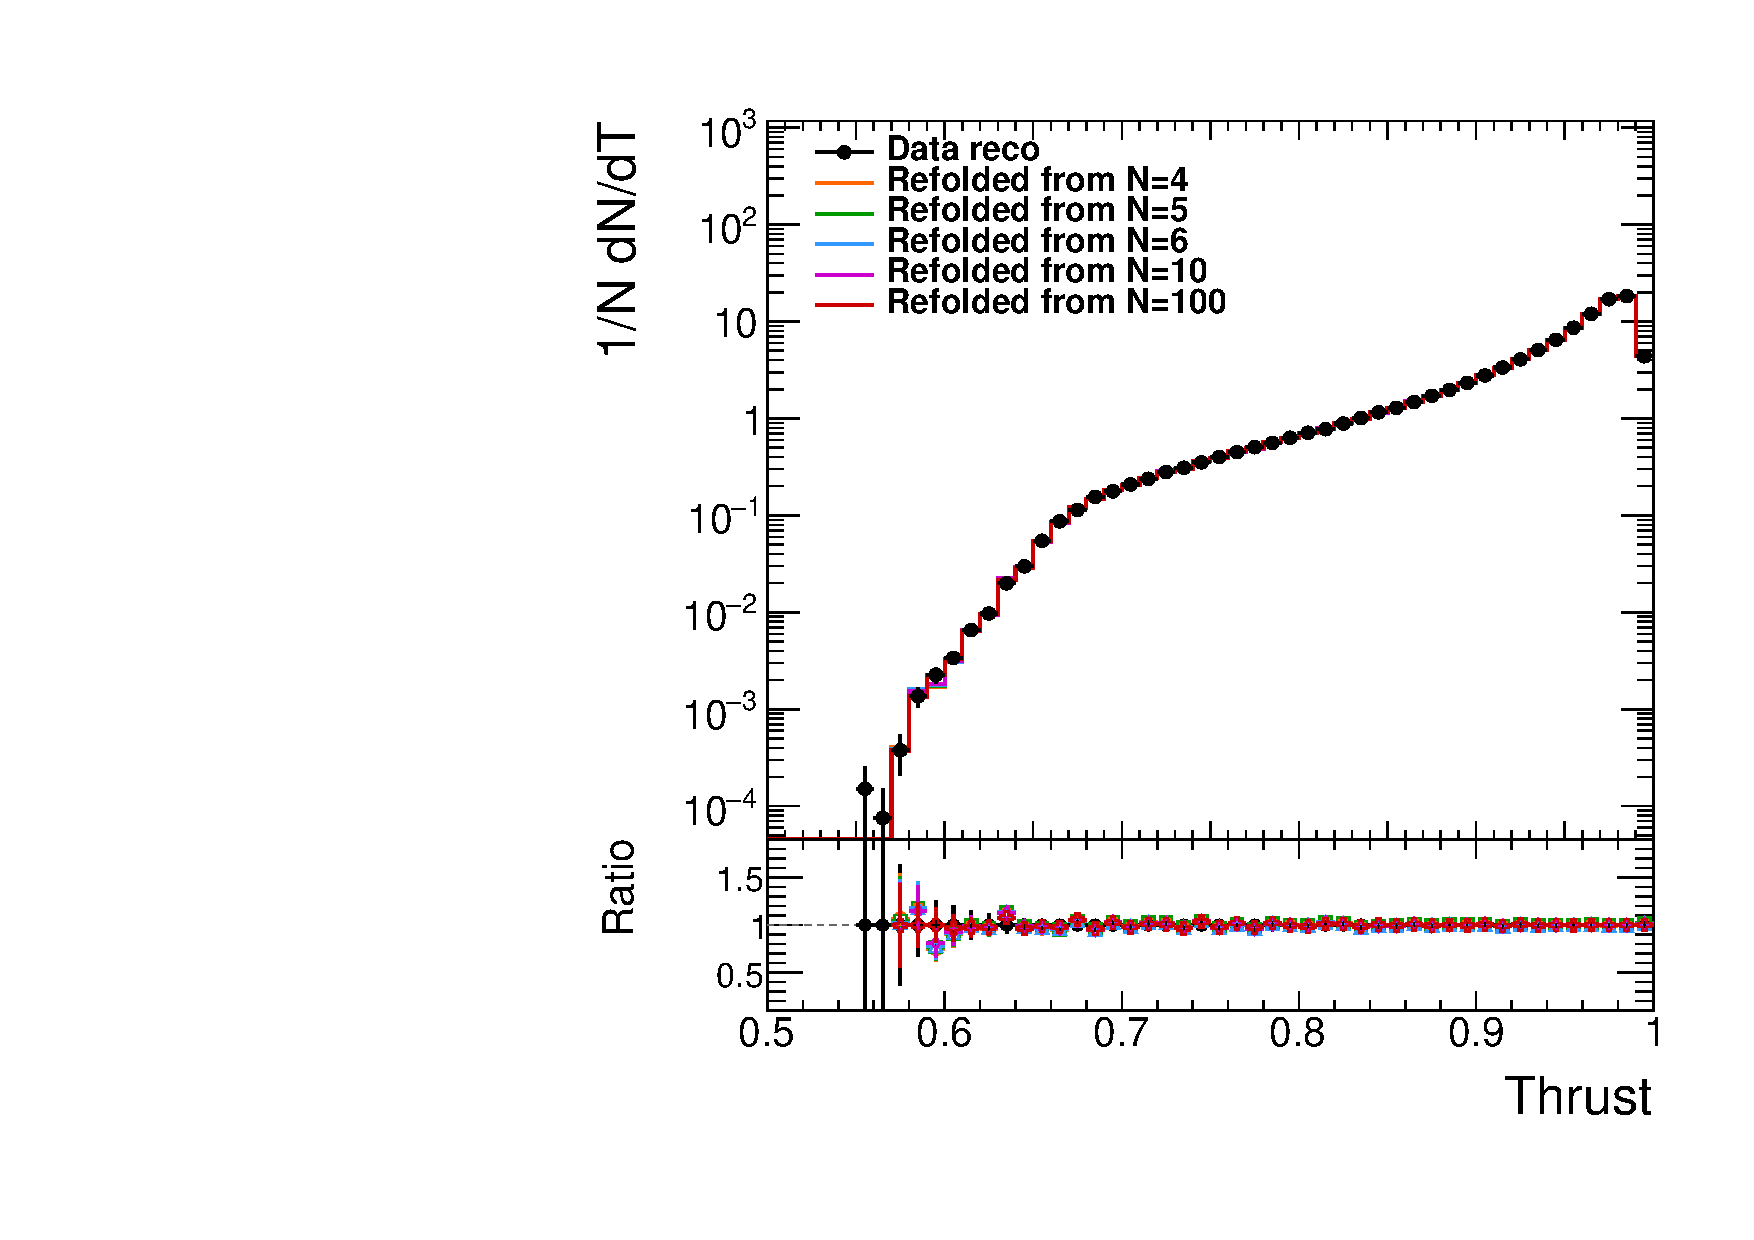
\includegraphics[width=0.65\textwidth]{../Studies/PreliminaryResult/2026-02-17_thrust_iter5/validation/iteration_scan/dist_refolded_vs_data_selected_iterations.pdf}
\caption{Refolded spectra from selected iteration points ($N_{\mathrm{iter}}=4,5,6,10,100$) compared with detector-level data.}
\label{fig:refold_selected_iters}
\end{figure}

\begin{figure}[t!]
\centering
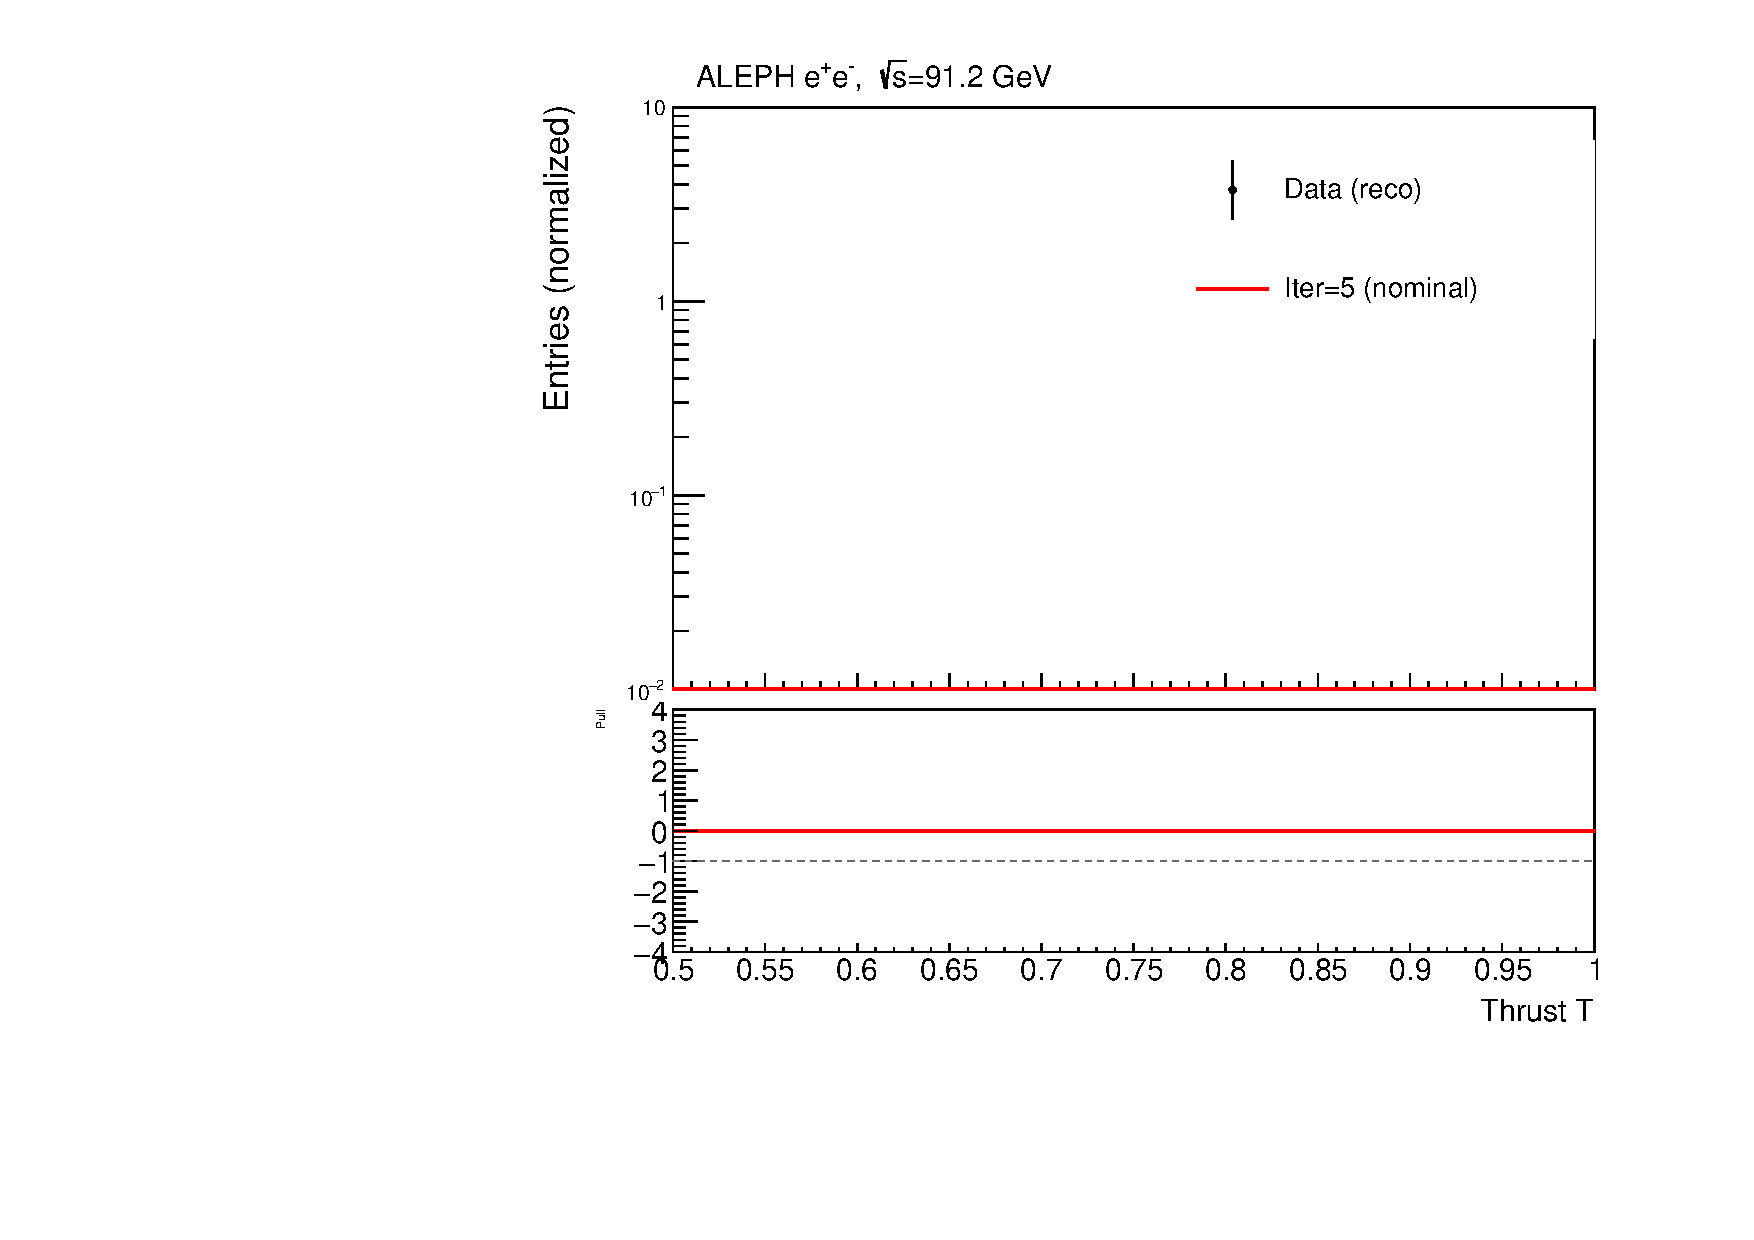
\includegraphics[width=0.65\textwidth]{../Studies/Phase2_Checks_2026-03-03/plots/pull_panel/dist_refolded_vs_data_pull.pdf}
\caption{Pull panel for refolded spectra: per-bin pull $(N_{\mathrm{data}} - N_{\mathrm{refold}})/\sigma$ for selected iteration points, showing bin-by-bin agreement between the detector-level data and each refolded prediction. Produced by \texttt{refolding\_pull\_panel.py} (see \texttt{Studies/Phase2\_Checks\_2026-03-03/}).}
\label{fig:refold_pull_panel}
\end{figure}

\begin{figure}[t!]
\centering
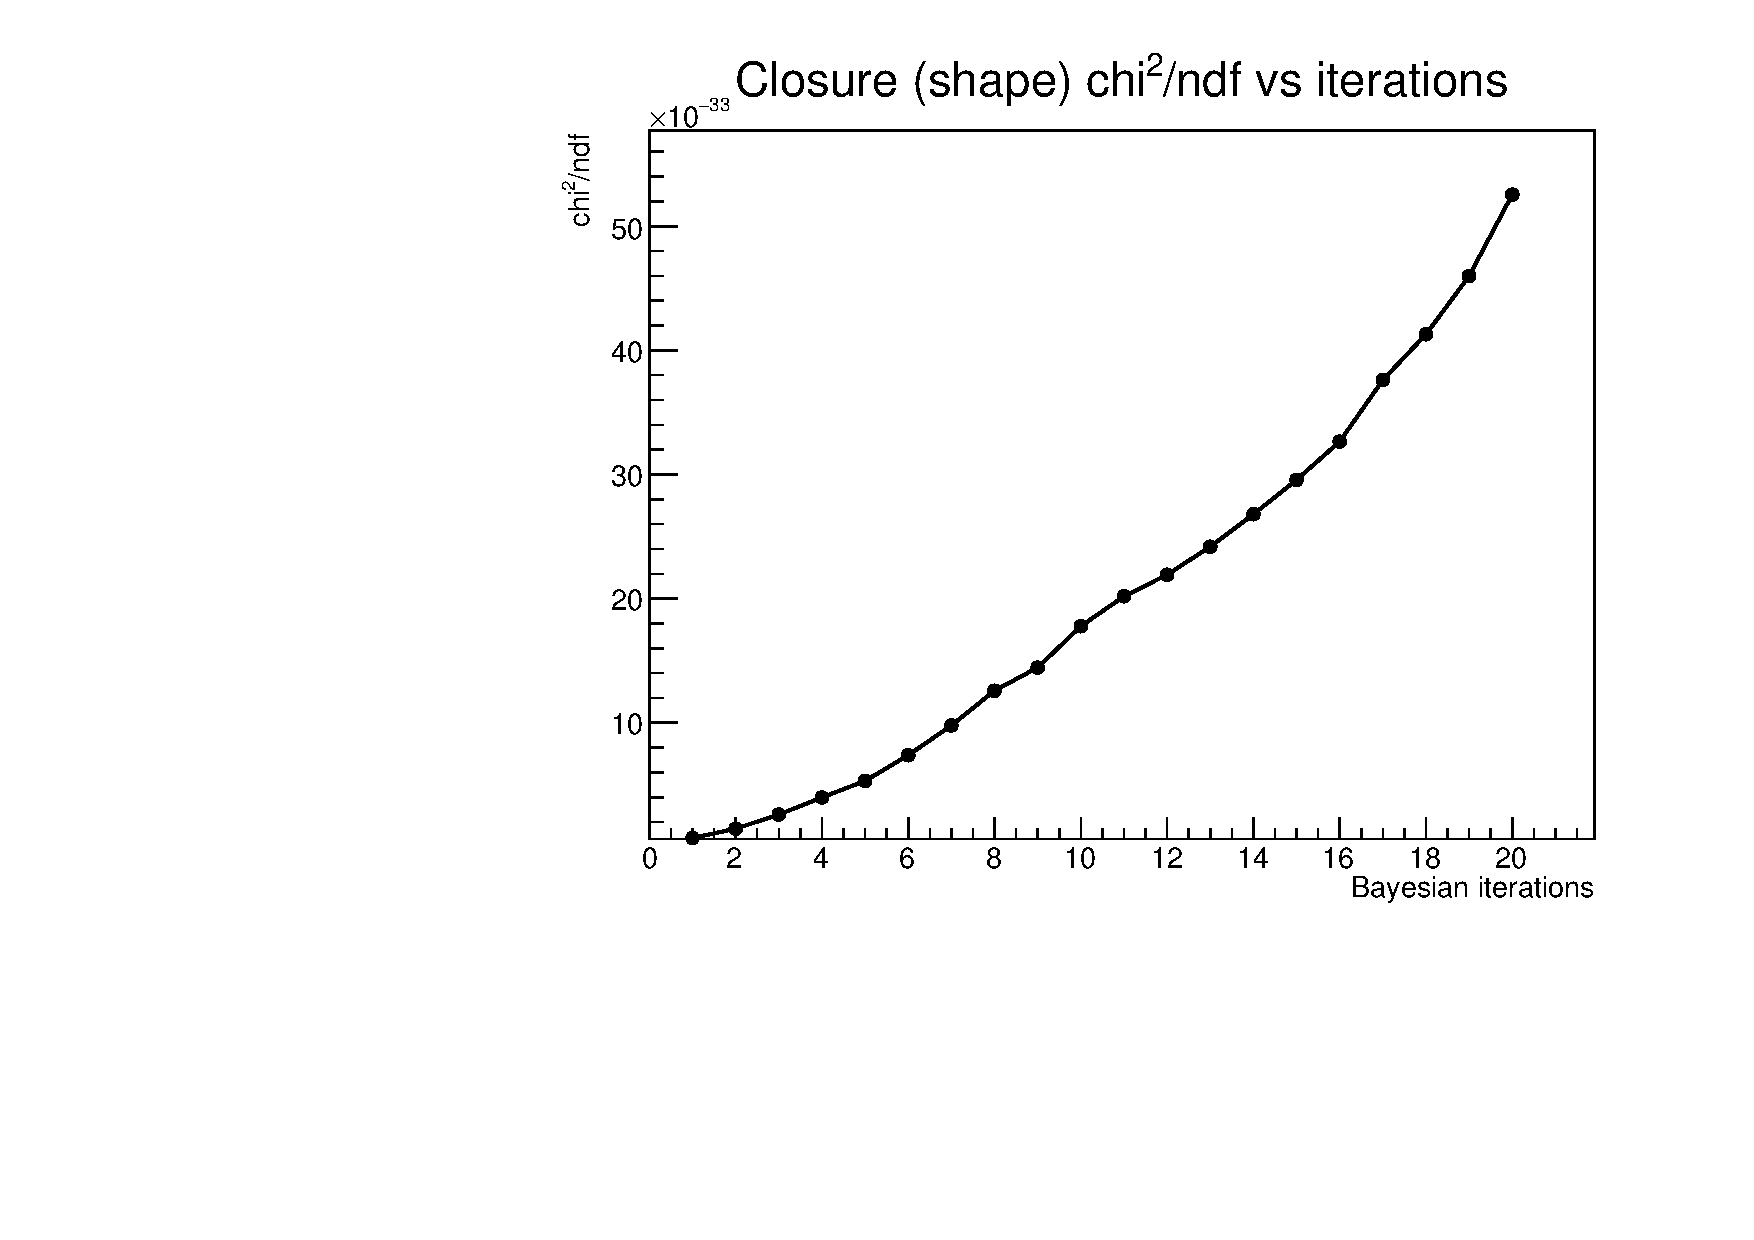
\includegraphics[width=0.49\textwidth]{../Studies/PreliminaryResult/2026-02-17_thrust_iter5/validation/iteration_scan/chi2ndf_closure_shape_vs_iterations.pdf}
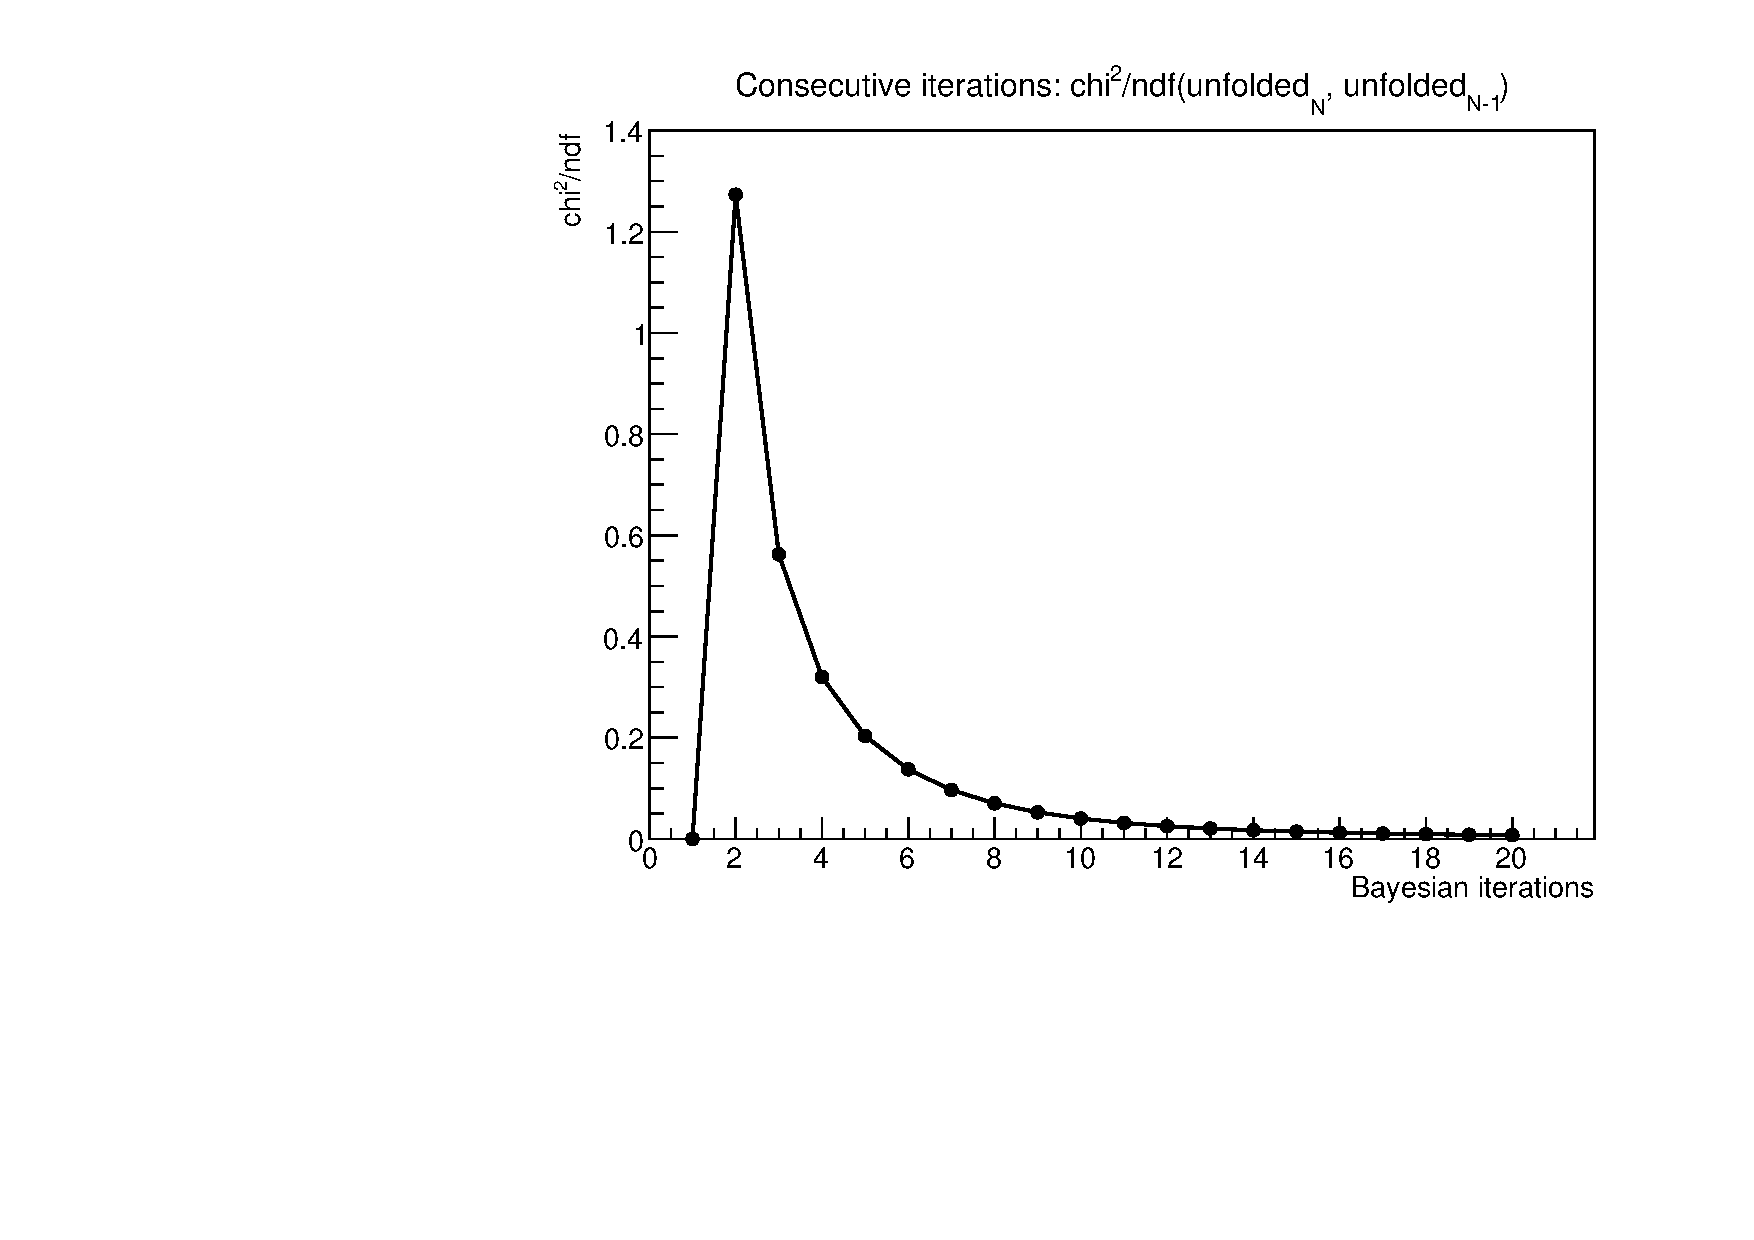
\includegraphics[width=0.49\textwidth]{../Studies/PreliminaryResult/2026-02-17_thrust_iter5/validation/iteration_scan/chi2ndf_iter_delta_counts_vs_iterations.pdf}
\\[2mm]
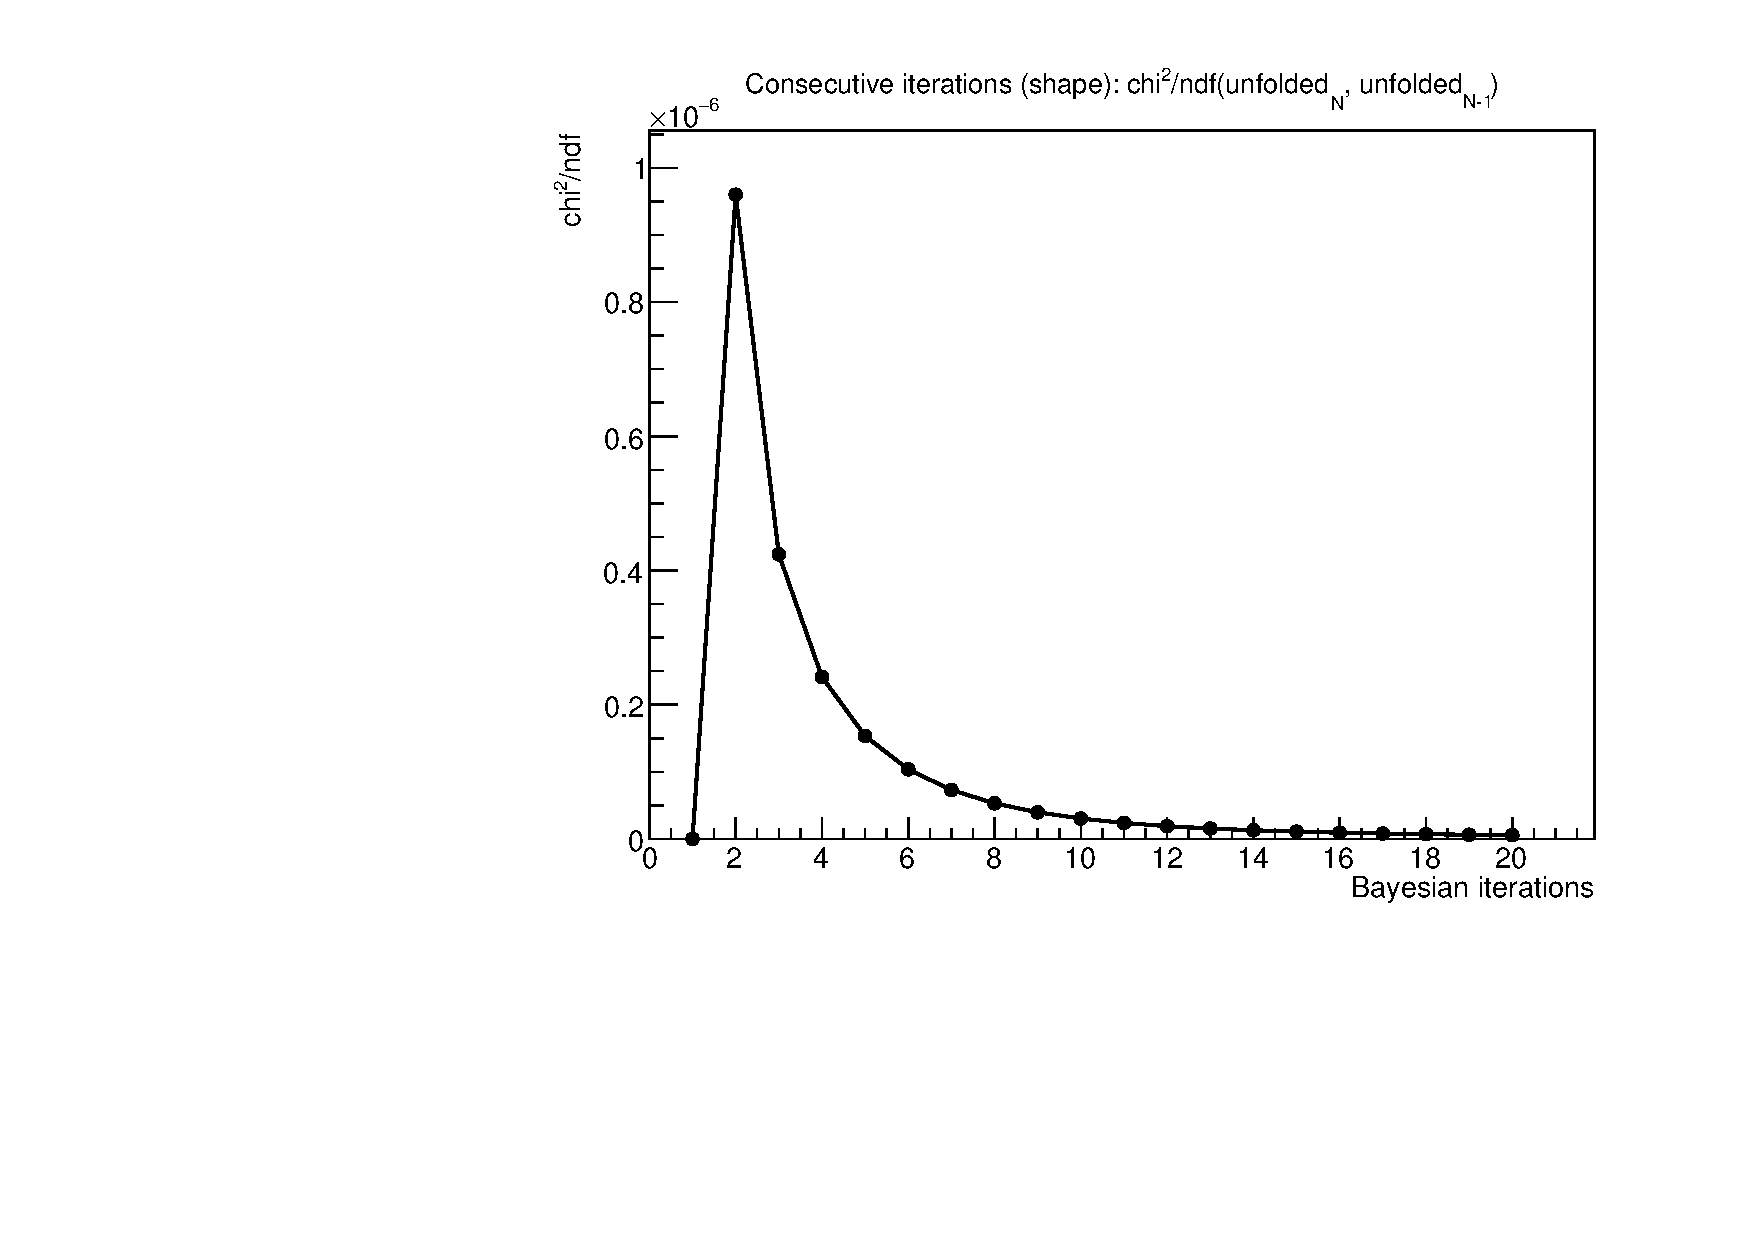
\includegraphics[width=0.49\textwidth]{../Studies/PreliminaryResult/2026-02-17_thrust_iter5/validation/iteration_scan/chi2ndf_iter_delta_shape_vs_iterations.pdf}
\caption{Iteration-choice diagnostics: closure-shape $\chi^2/\mathrm{ndf}$ (top left), iteration-to-iteration count-level stability (top right), and iteration-to-iteration shape stability (bottom left).}
\label{fig:iteration_choice_diagnostics}
\end{figure}

\FloatBarrier

\subsection{Thrust resolution study}
\label{sec:thrust_resolution}

The usable binning resolution varies across the thrust spectrum. To quantify this,
we use the matched reco--gen event pairs to study the thrust resolution as a function
of true thrust. Specifically, we plot $(T_{\mathrm{reco}} - T_{\mathrm{gen}})$ versus
$T_{\mathrm{gen}}$ in a two-dimensional histogram, and extract the resolution
$\sigma(T)$ as a function of $T_{\mathrm{gen}}$ from the per-slice width of the
$(T_{\mathrm{reco}} - T_{\mathrm{gen}})$ distribution. This study is particularly
important in the high-thrust (low $\tau = 1-T$) regime, which spans the peak of the
thrust distribution and the deep non-perturbative region. The previous ALEPH
analyses~\cite{Heister:2003aj} chose bin sizes to be ``somewhat smaller than twice
the corresponding detector resolution,'' and our IBU approach, while less sensitive
to binning than the matrix method, still uses this principle to guide the finest
bins tested in the region.

\begin{figure}[t!]
\centering
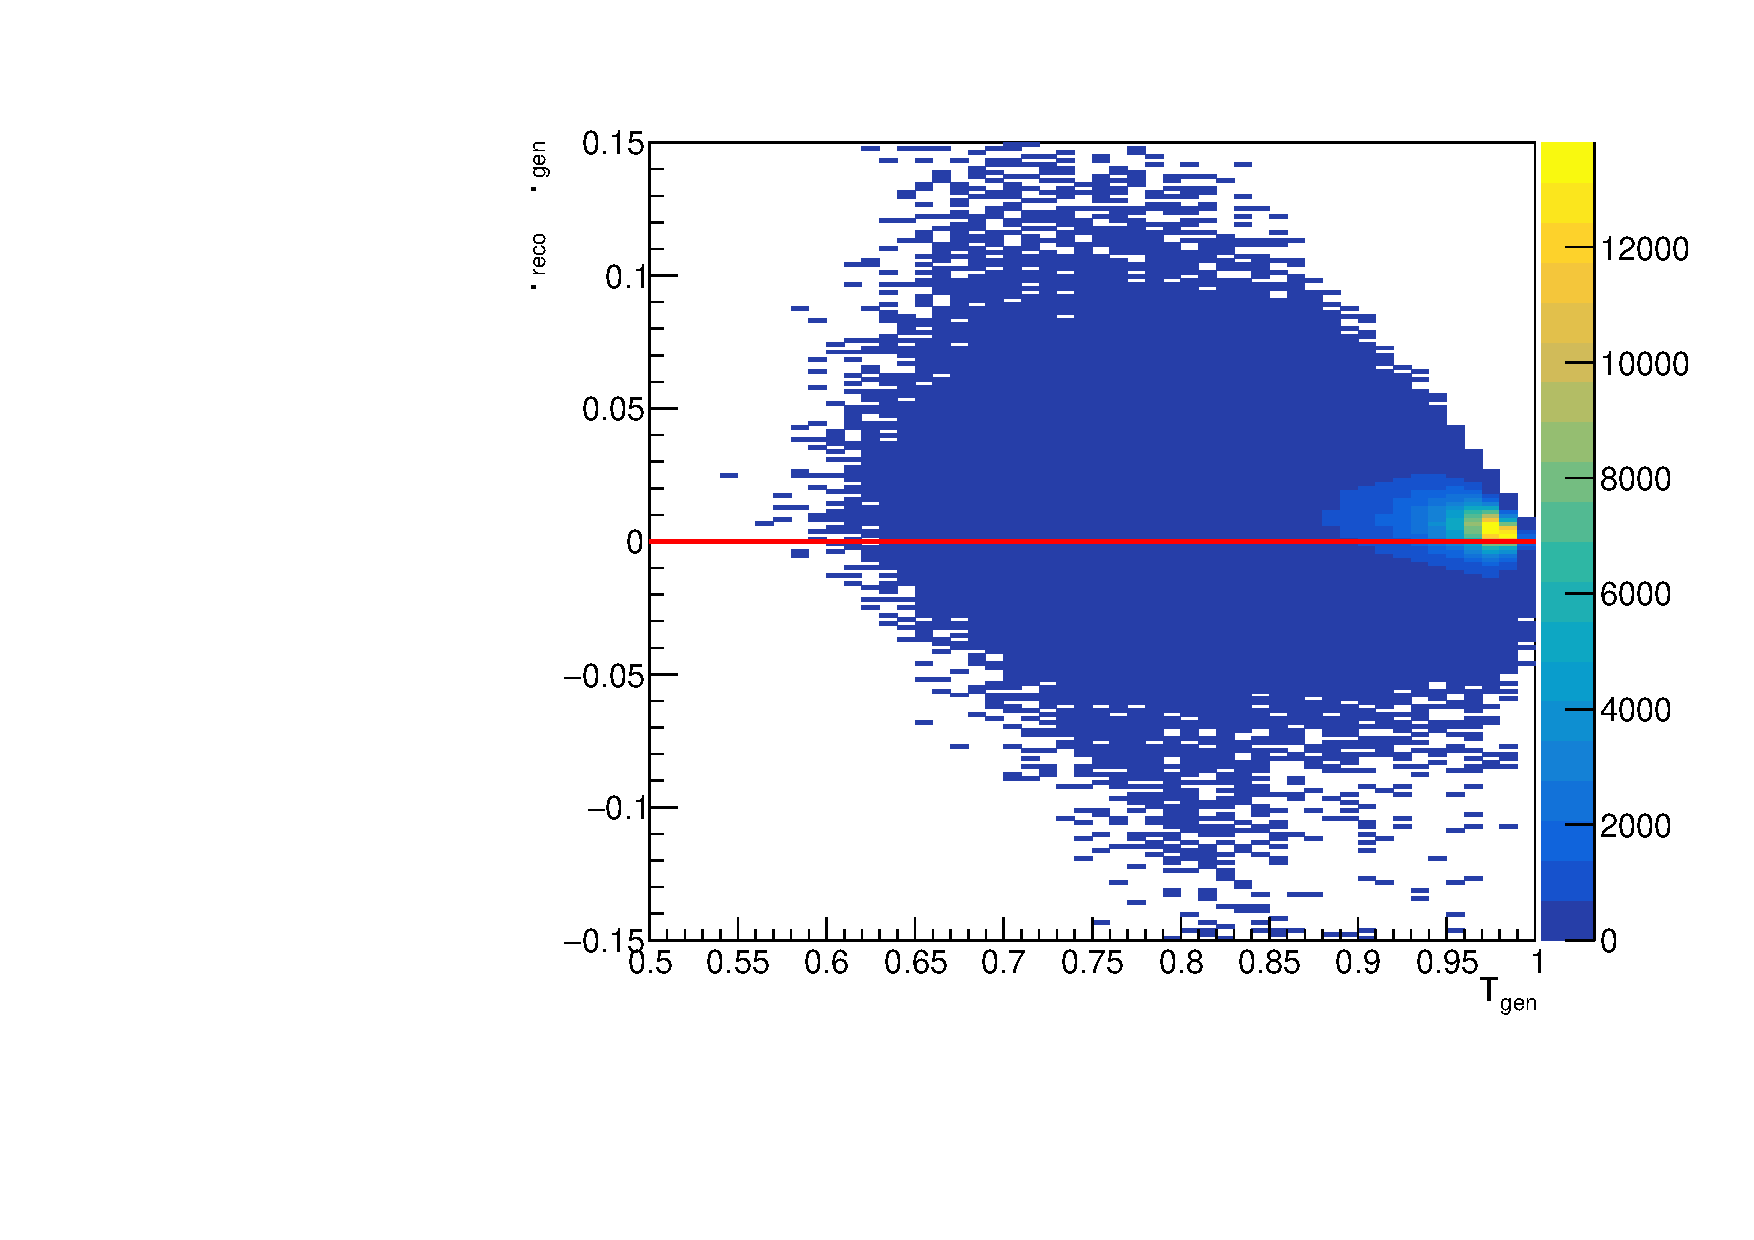
\includegraphics[width=0.60\textwidth]{../Studies/Phase2_Checks_2026-03-03/plots/thrust_resolution/thrust_resolution_2d.pdf}
\caption{Two-dimensional distribution of $(T_{\mathrm{reco}}-T_{\mathrm{gen}})$ vs $T_{\mathrm{gen}}$ for matched MC event pairs. The spread narrows toward $T\to1$ (low-$\tau$ region), motivating finer binning there.}
\label{fig:thrust_resolution_2d}
\end{figure}

\begin{figure}[t!]
\centering
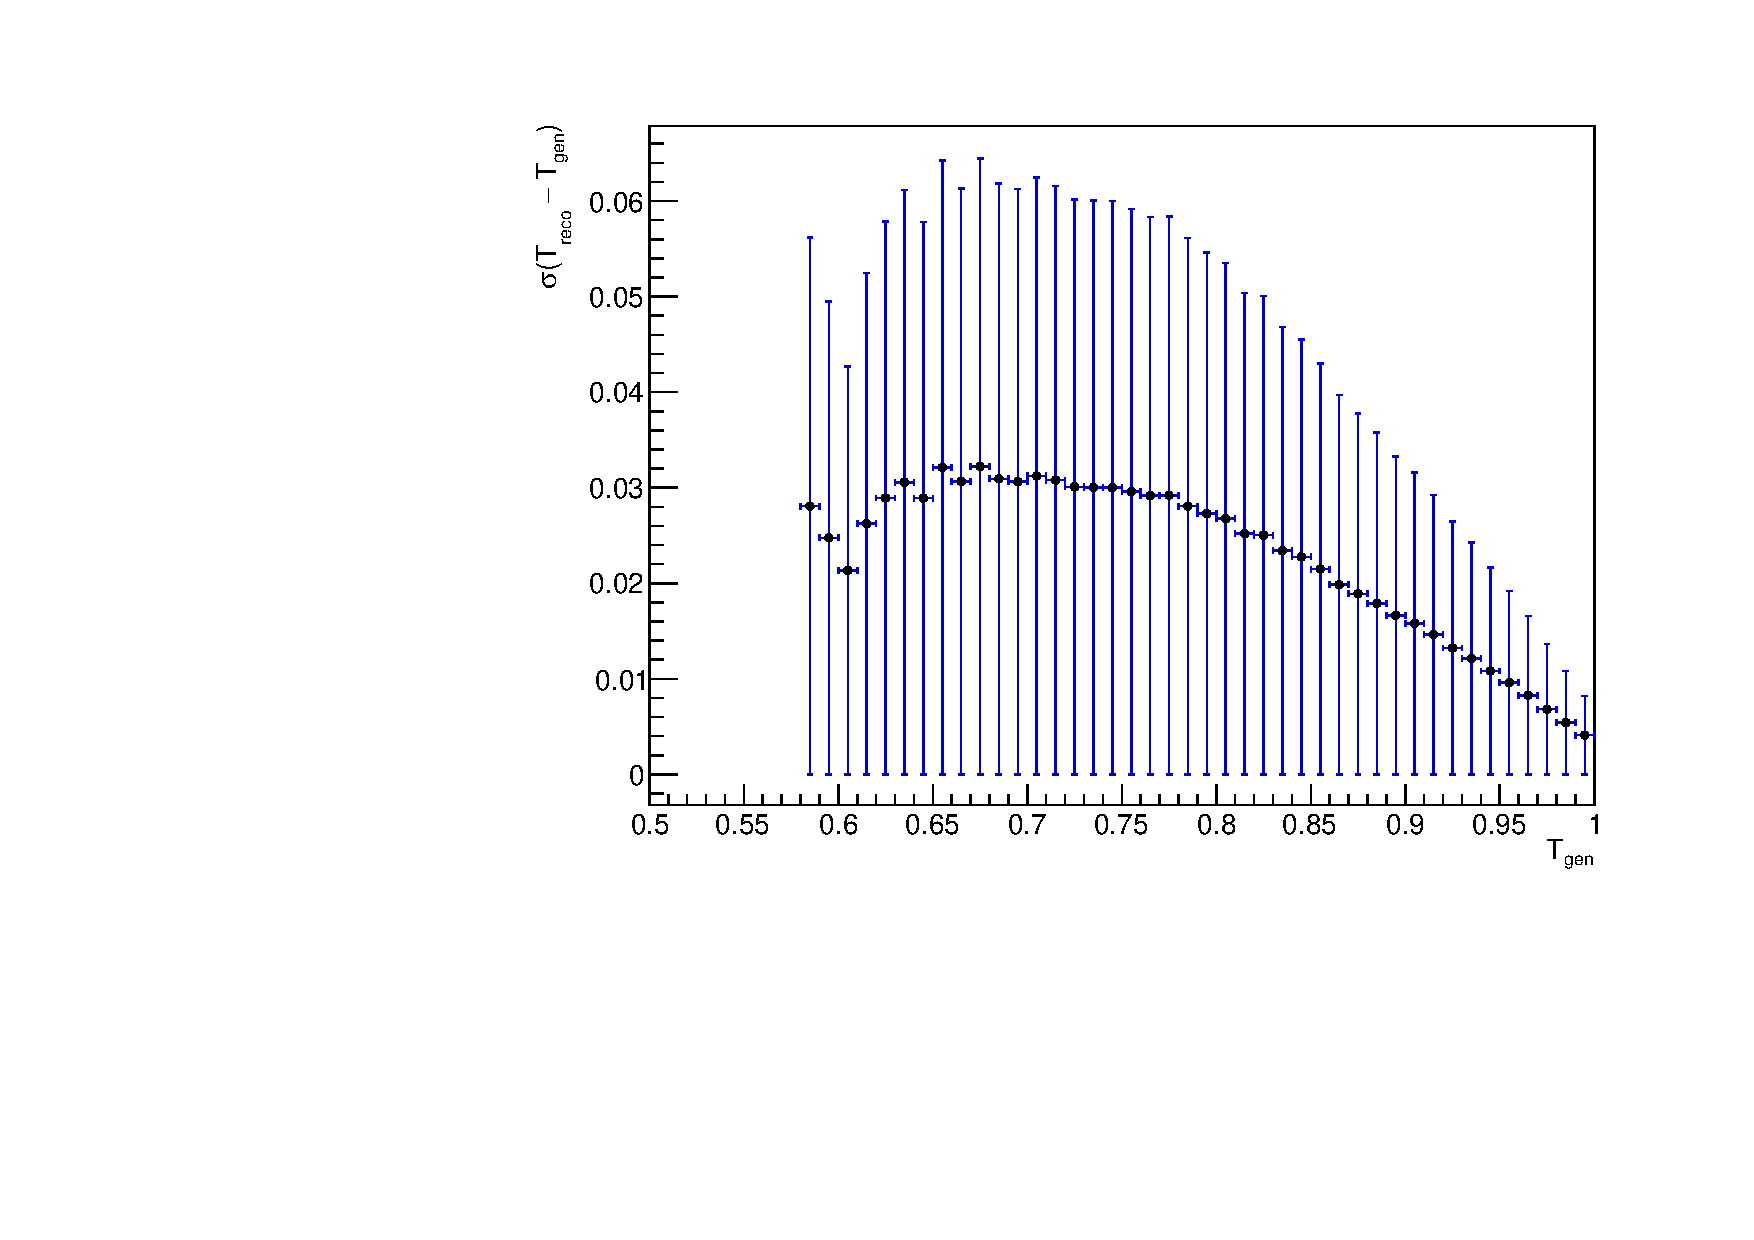
\includegraphics[width=0.49\textwidth]{../Studies/Phase2_Checks_2026-03-03/plots/thrust_resolution/thrust_resolution_profile.pdf}
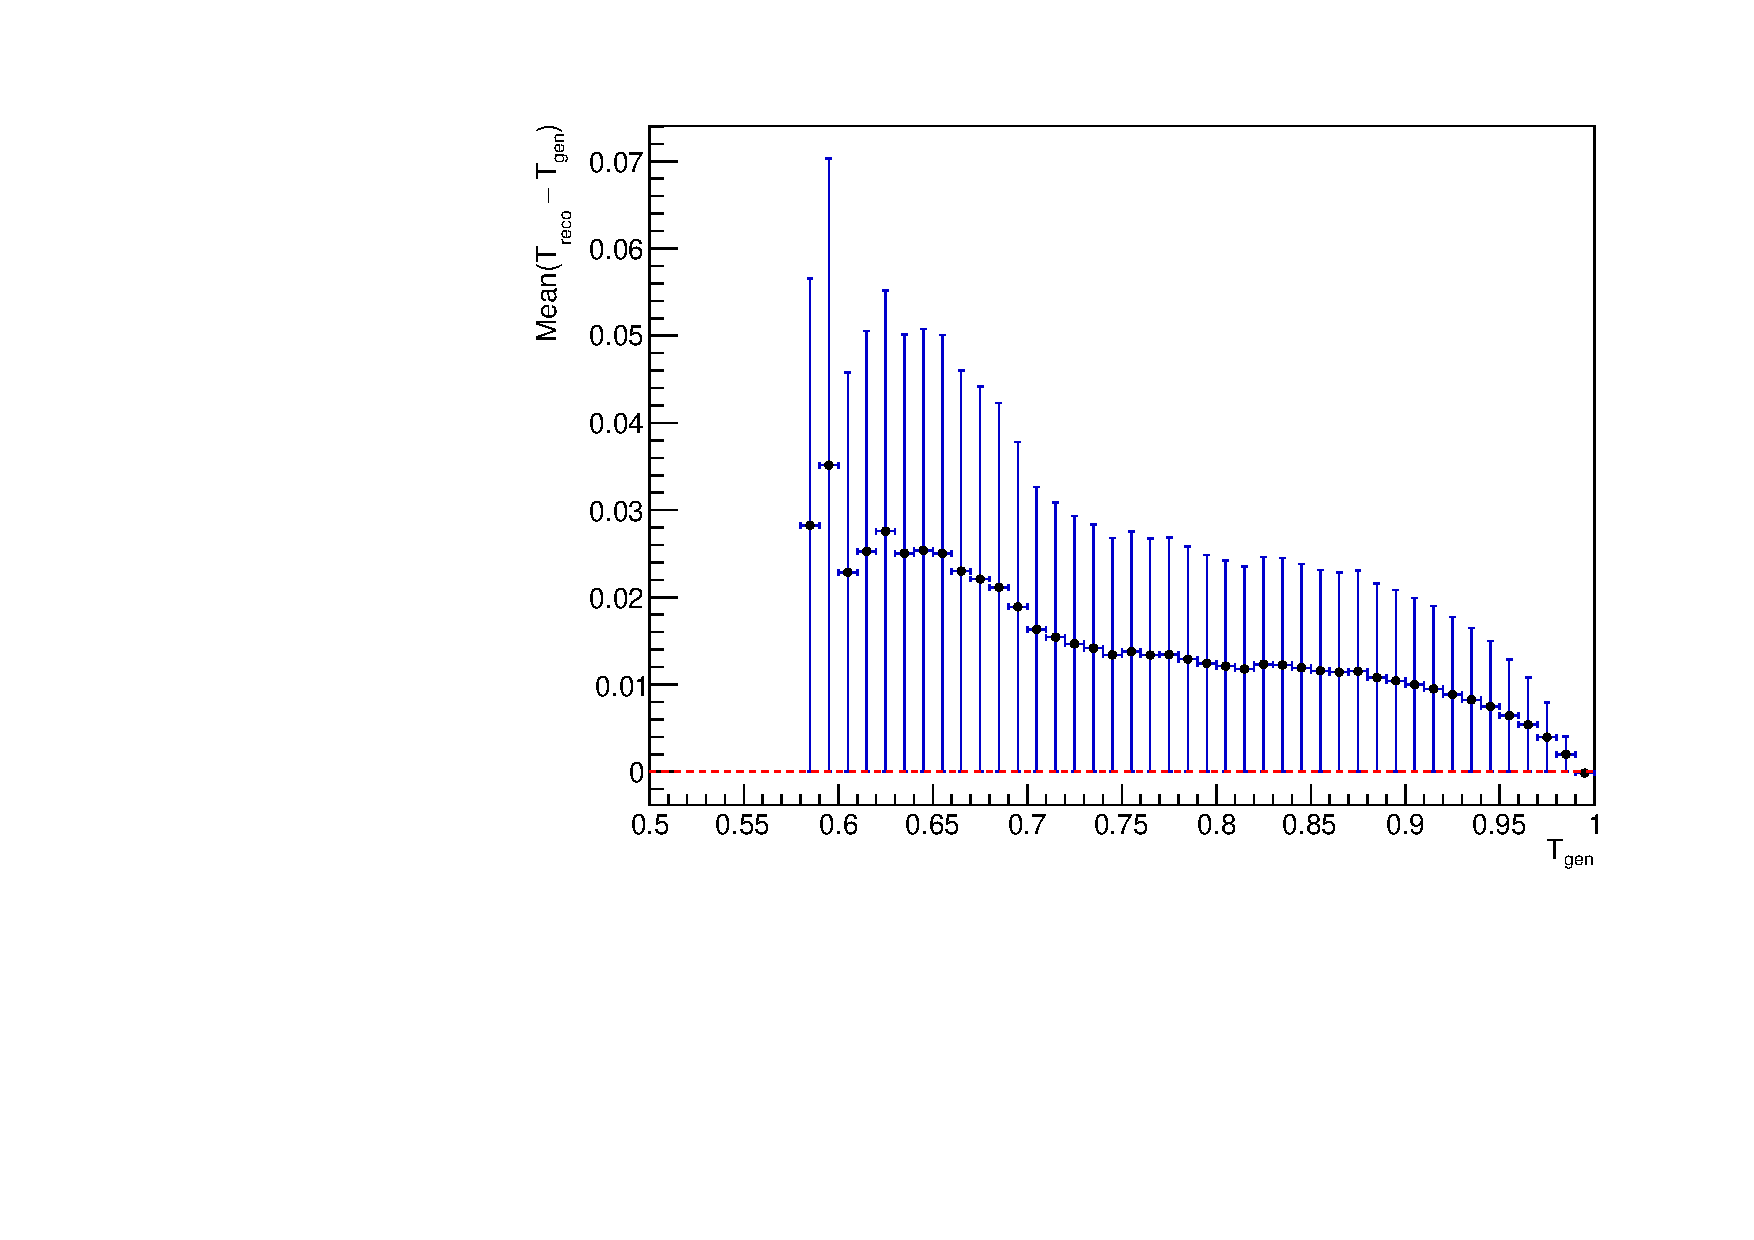
\includegraphics[width=0.49\textwidth]{../Studies/Phase2_Checks_2026-03-03/plots/thrust_resolution/thrust_resolution_bias.pdf}
\caption{Left: per-slice RMS of $(T_{\mathrm{reco}}-T_{\mathrm{gen}})$ as a function of $T_{\mathrm{gen}}$, giving the thrust resolution profile $\sigma(T)$. Right: mean bias $\langle T_{\mathrm{reco}}-T_{\mathrm{gen}}\rangle$ vs $T_{\mathrm{gen}}$; values consistent with zero indicate no systematic shift.}
\label{fig:thrust_resolution_profile}
\end{figure}

\subsection{Systematics execution map}

Systematic branches are executed by rerunning unfolding with variation-specific inputs or theory weights, then converting each branch into a signed shift relative to nominal.
The combination structure is summarized in Table~\ref{fig:systematics_execution_chart}.

\begin{figure}[t!]
\centering
\resizebox{0.98\linewidth}{!}{%
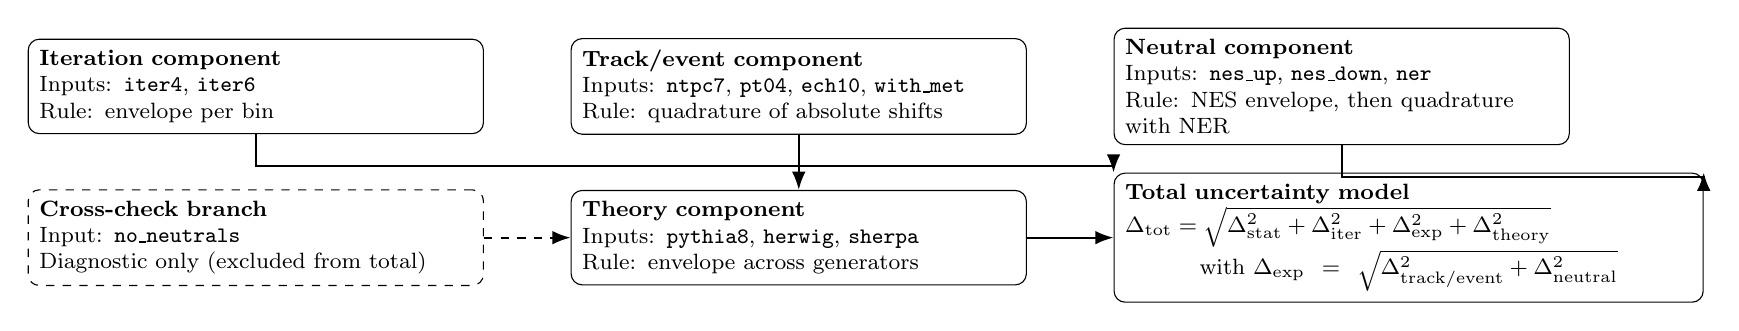
\begin{tikzpicture}[
  >=Latex,
  node distance=6mm,
  every node/.style={font=\footnotesize},
  block/.style={draw, rounded corners, align=left, text width=5.5cm, inner sep=4pt},
  merge/.style={draw, rounded corners, align=center, text width=7.2cm, inner sep=4pt},
  diag/.style={draw, rounded corners, align=left, text width=5.5cm, inner sep=4pt, dashed},
  arrow/.style={-Latex, line width=0.8pt}
]

\node[block] (iter) {\textbf{Iteration component}\newline
Inputs: \texttt{iter4}, \texttt{iter6}\newline
Rule: envelope per bin};

\node[block, right=11mm of iter] (track) {\textbf{Track/event component}\newline
Inputs: \texttt{ntpc7}, \texttt{pt04}, \texttt{ech10}, \texttt{with\_met}\newline
Rule: quadrature of absolute shifts};

\node[block, right=11mm of track] (neutral) {\textbf{Neutral component}\newline
Inputs: \texttt{nes\_up}, \texttt{nes\_down}, \texttt{ner}\newline
Rule: NES envelope, then quadrature with NER};

\node[block, below=7mm of track] (theory) {\textbf{Theory component}\newline
Inputs: \texttt{pythia8}, \texttt{herwig}, \texttt{sherpa}\newline
Rule: envelope across generators};

\node[diag, left=11mm of theory] (noneu) {\textbf{Cross-check branch}\newline
Input: \texttt{no\_neutrals}\newline
Diagnostic only (excluded from total)};

\node[merge, right=11mm of theory] (total) {\textbf{Total uncertainty model}\newline
$\Delta_{\mathrm{tot}}=\sqrt{\Delta_{\mathrm{stat}}^2+\Delta_{\mathrm{iter}}^2+\Delta_{\mathrm{exp}}^2+\Delta_{\mathrm{theory}}^2}$\newline
with $\Delta_{\mathrm{exp}}=\sqrt{\Delta_{\mathrm{track/event}}^2+\Delta_{\mathrm{neutral}}^2}$};

\draw[arrow] (iter.south) -- ++(0,-4mm) -| (total.north west);
\draw[arrow] (track.south) -- ++(0,-4mm) -- (theory.north);
\draw[arrow] (neutral.south) -- ++(0,-4mm) -| (total.north east);
\draw[arrow] (theory.east) -- (total.west);
\draw[arrow, dashed] (noneu.east) -- (theory.west);

\end{tikzpicture}
}
\caption{Systematics combination chart for the thrust baseline. Solid arrows indicate components entering the nominal total uncertainty; dashed branch is the reported stress-test excluded from total.}
\label{fig:systematics_execution_chart}
\end{figure}


The nominal total uncertainty model (Sec.~\ref{sec:systematics}) combines component magnitudes in quadrature after branch-specific envelope or quadrature rules.
The \texttt{no\_neutrals} branch is retained as a stress-test and explicitly reported, but excluded from the nominal total.

\subsection{Hadronic correction, covariance propagation, and matrix exports}

After unfolding, a bin-wise hadronic event-selection correction is applied,
\begin{equation}
C_{\mathrm{had}}(j)=\frac{N_{\mathrm{genBefore}}(j)}{N_{\mathrm{gen}}(j)},
\qquad
U_j^{\mathrm{corr}} = U_j\,C_{\mathrm{had}}(j).
\end{equation}

For the nominal run, the statistical covariance is computed by RooUnfold using analytical error propagation (\texttt{RooUnfold::kCovariance}), which propagates Poisson uncertainties in the data and response histograms through the IBU iteration chain without toy MC sampling. The resulting covariance matrix is read from the unfolding output and transformed to the normalized differential-thrust basis used in this note. Non-statistical component covariances are built with a configurable model (nominal: \texttt{template\_correlated}), and fit-window covariance products are exported together with full-range matrices by
\texttt{build\_prelim\_uncertainty\_summary.py}.

Response and matrix visualizations are exported by the matrix-plot helper script (see Appendix~\ref{sec:app_workflow_code} for details). Full provenance metadata for the run, including git commit, ROOT version, RooUnfold version, environment fingerprint, response diagnostics, theory-weight coverage, and all computed uncertainty metrics, is written to a structured JSON summary file. This file is the primary machine-readable record of the result and is the canonical reference for any numeric claims in Sec.~\ref{sec:results}.

\begin{figure}[t!]
\centering
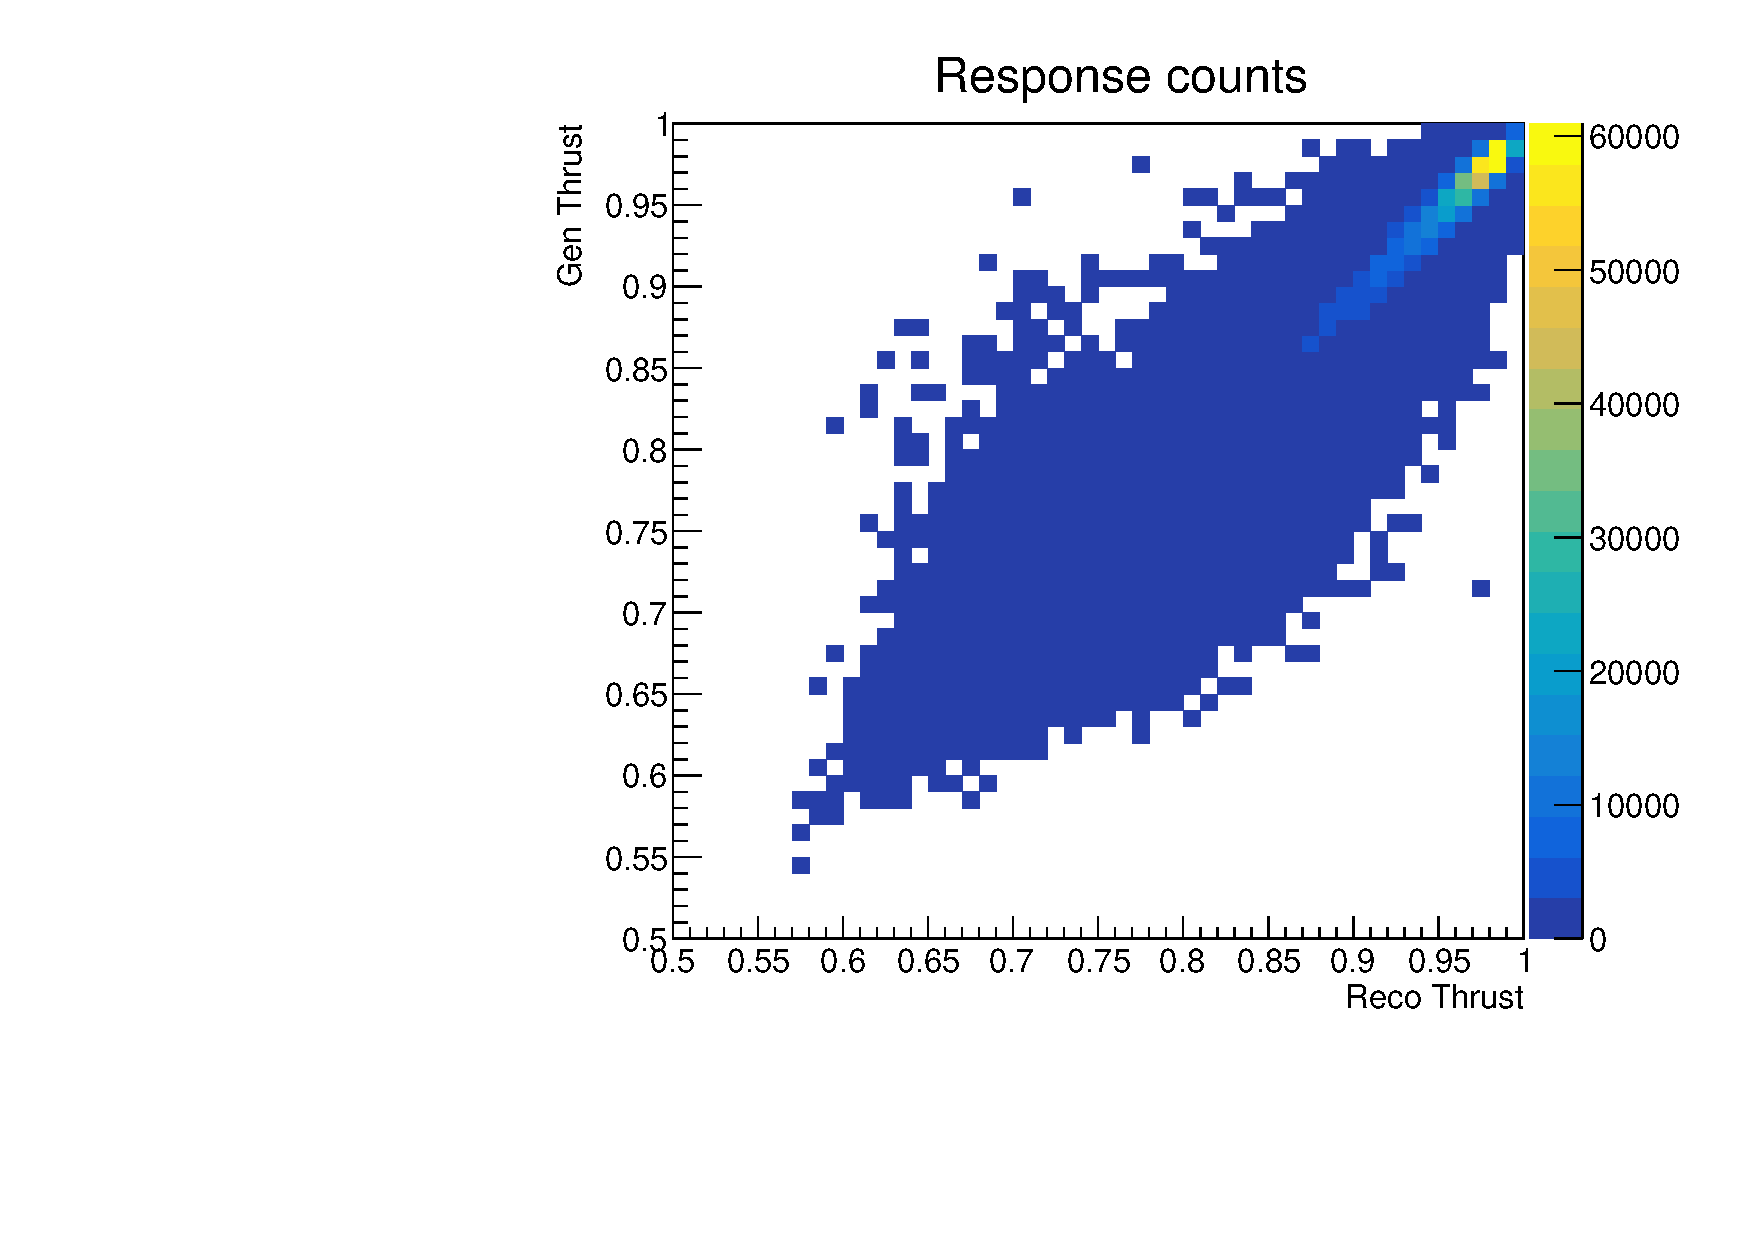
\includegraphics[width=0.49\textwidth]{../Studies/PreliminaryResult/2026-02-17_thrust_iter5/summary/matrices_nominal_iter5/matrix_response_counts.pdf}
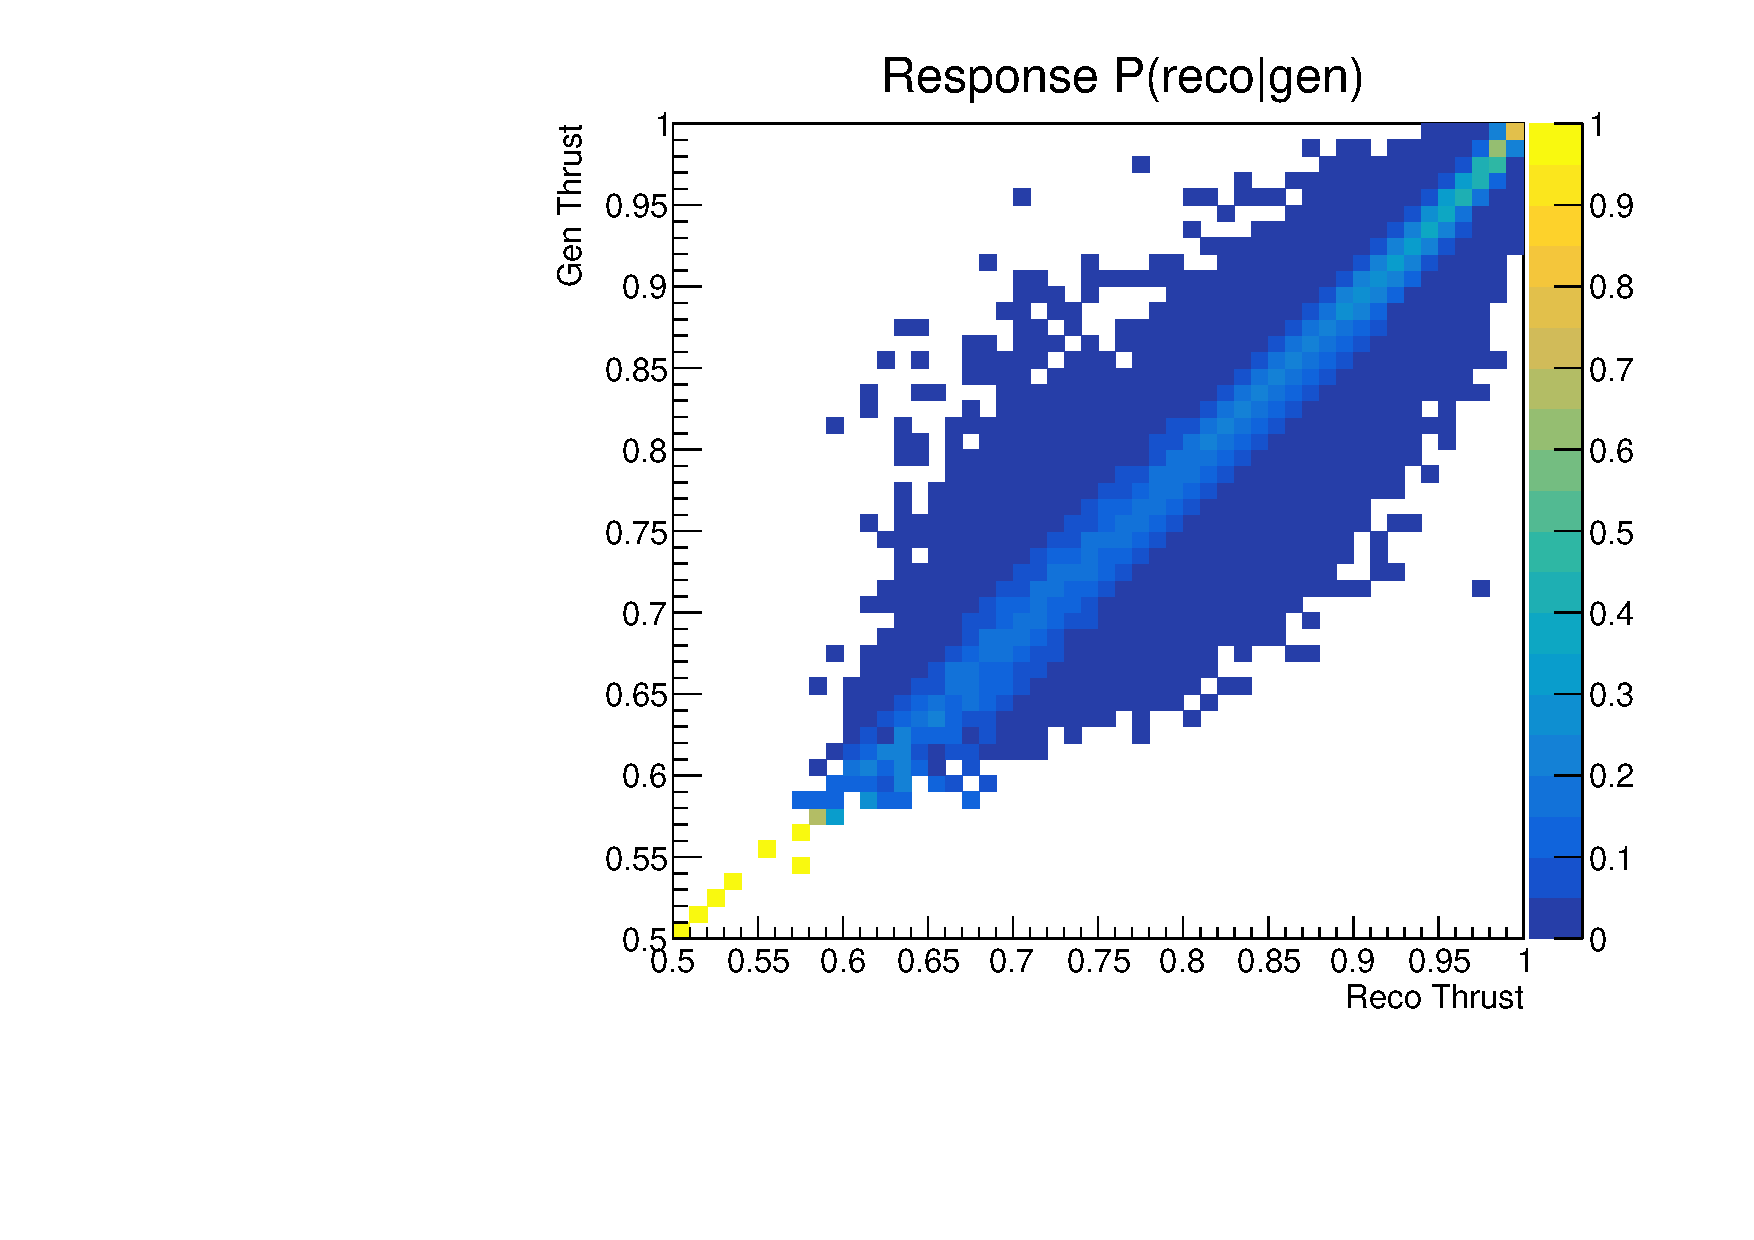
\includegraphics[width=0.49\textwidth]{../Studies/PreliminaryResult/2026-02-17_thrust_iter5/summary/matrices_nominal_iter5/matrix_response_probability.pdf}
\caption{Nominal response matrices for thrust: response counts (left) and response probability (right).}
\label{fig:response_matrices_nominal}
\end{figure}

\begin{figure}[t!]
\centering
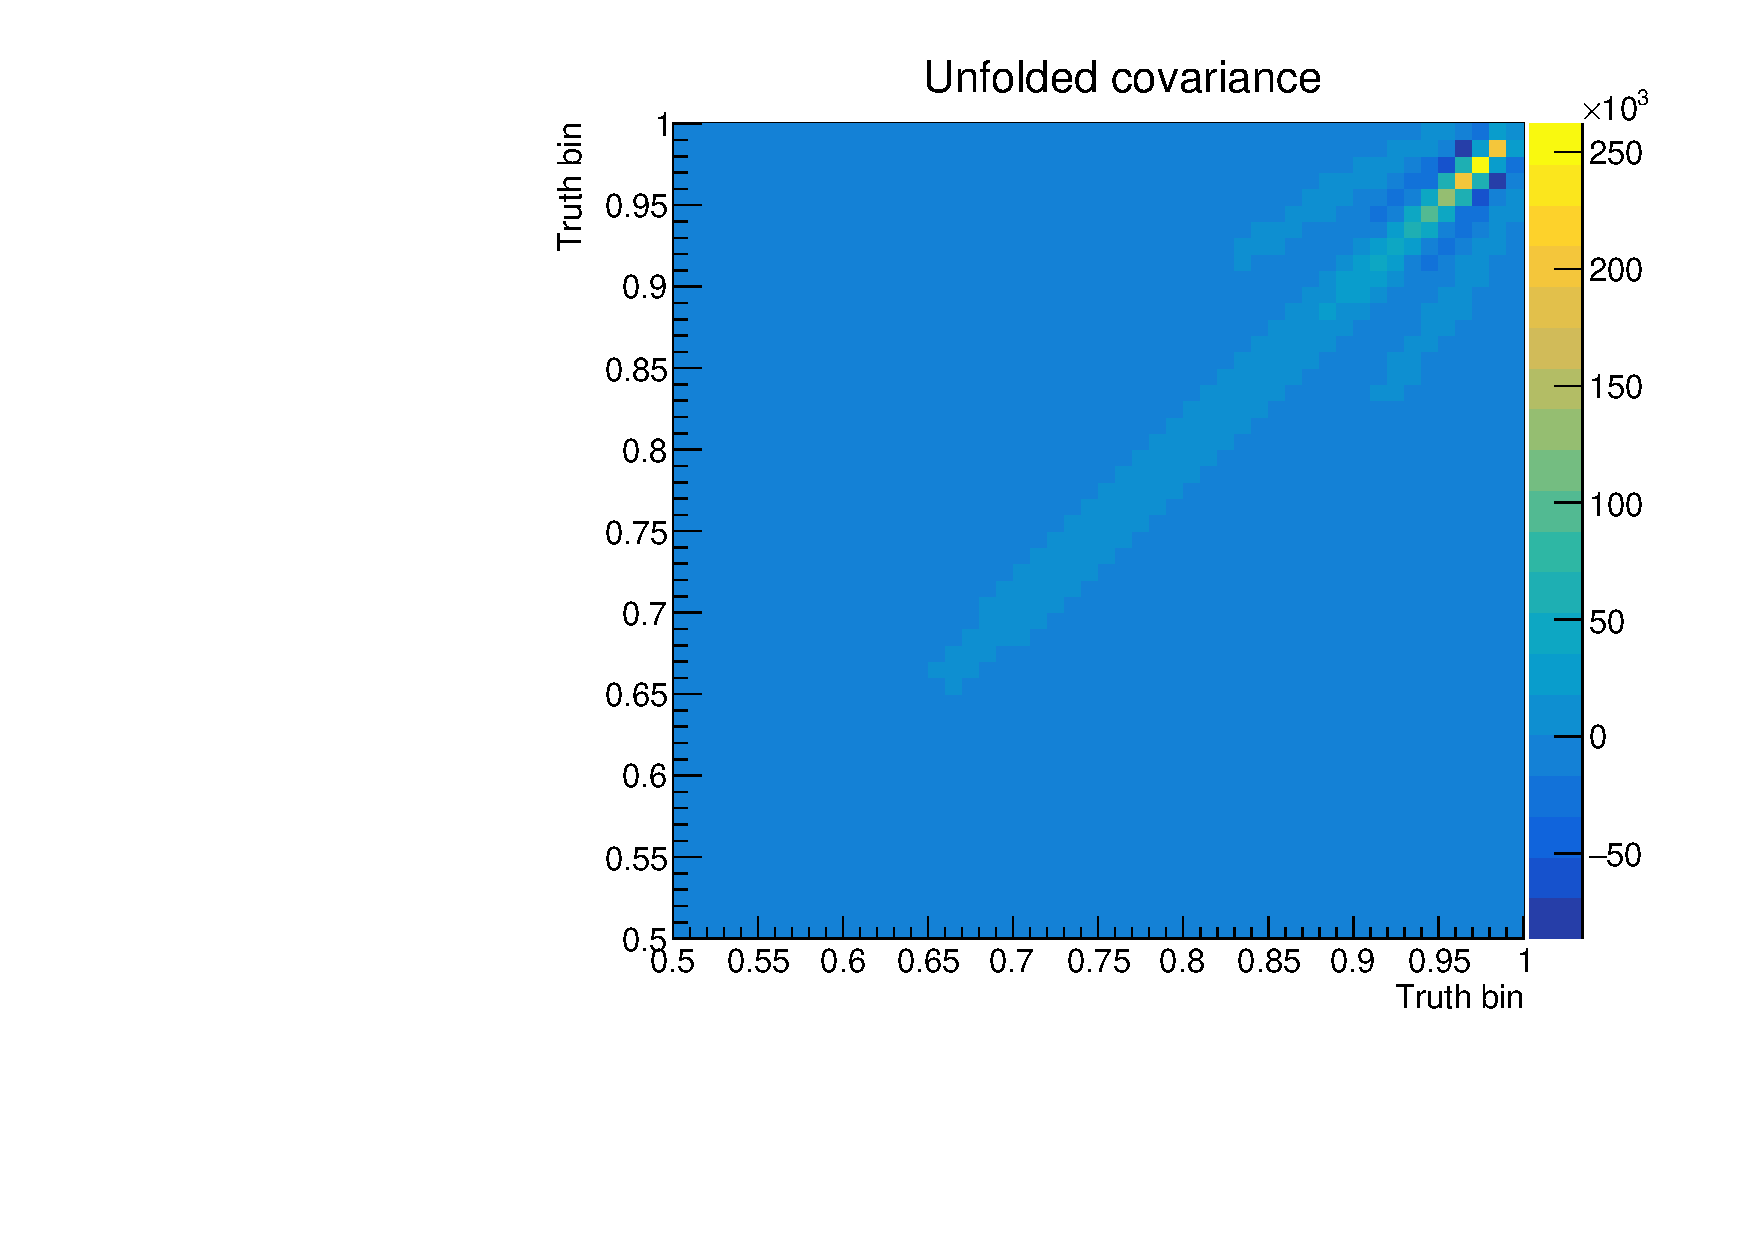
\includegraphics[width=0.49\textwidth]{../Studies/PreliminaryResult/2026-02-17_thrust_iter5/summary/matrices_nominal_iter5/matrix_unfold_covariance.pdf}
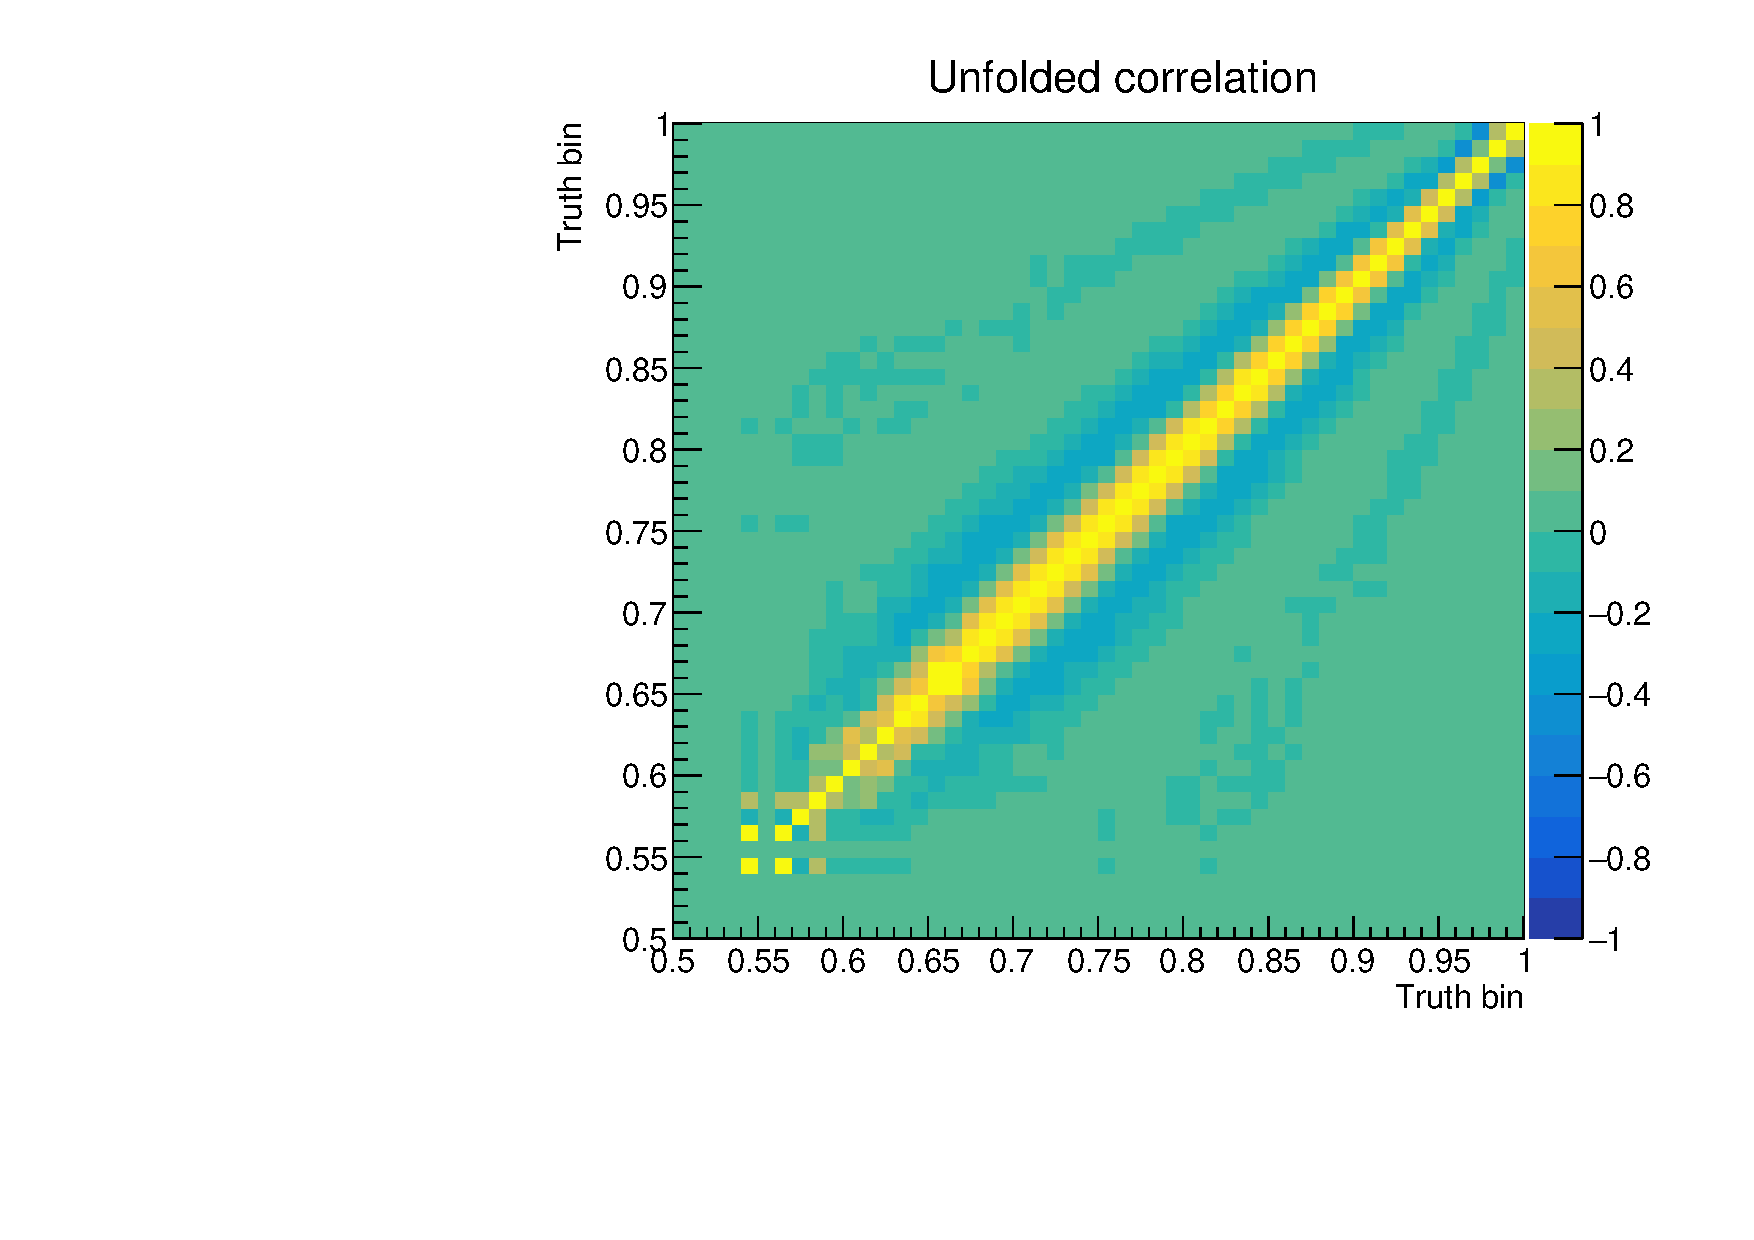
\includegraphics[width=0.49\textwidth]{../Studies/PreliminaryResult/2026-02-17_thrust_iter5/summary/matrices_nominal_iter5/matrix_unfold_correlation.pdf}
\caption{Nominal unfolded covariance matrix (left) and corresponding correlation matrix (right).}
\label{fig:covariance_correlation_nominal}
\end{figure}

The nominal and systematics execution logic, including command sequences, pseudocode for workflow control and uncertainty assembly, and the reproduction contract for this note, are documented in Appendix~\ref{sec:app_workflow_code}.

\section{Systematic uncertainties}
\label{sec:systematics}

Systematic variations are propagated by rerunning the full unfolding chain for each variation and comparing to the nominal unfolded result. The implementation uses:
\begin{itemize}
\item \texttt{run\_thrust\_prelim\_workflow.py} for branch execution;
\item \texttt{build\_prelim\_uncertainty\_summary.py} for component extraction and total combination.
\end{itemize}
For each source $v$, the signed bin-wise shift is
\begin{equation}
\delta_v(j)=\frac{U_v(j)-U_{\mathrm{nom}}(j)}{U_{\mathrm{nom}}(j)}.
\end{equation}

\begin{table}[t!]
\centering
\scriptsize
\begin{tabularx}{0.98\textwidth}{p{0.19\textwidth}p{0.14\textwidth}p{0.31\textwidth}X}
\hline
Group & Source & Physics motivation & Combination in $\Delta_\mathrm{tot}$ \\
\hline
Unfolding regularization
  & \texttt{iter4}, \texttt{iter6}
  & Tests sensitivity to regularization strength; probes potential d'Agostini bias from under- or over-iteration
  & envelope: $\max(|\delta_{4}|,|\delta_{6}|)$ \\[3pt]
Track/event (1 of 4)
  & \texttt{ntpc7}
  & Tightens TPC hit requirement ($N_\mathrm{TPC}>7$ vs.\ nominal $>4$); probes tracking quality sensitivity
  & quadrature of all four absolute shifts \\[3pt]
Track/event (2 of 4)
  & \texttt{pt04}
  & Raises charged $p_T$ threshold ($>0.4$ GeV vs.\ nominal $>0.2$ GeV); probes soft-track contribution to thrust
  & (same) \\[3pt]
Track/event (3 of 4)
  & \texttt{ech10}
  & Lowers charged-energy requirement ($>10$ GeV vs.\ nominal $>15$ GeV); probes selection-boundary sculpting near hadronic-event threshold
  & (same) \\[3pt]
Track/event (4 of 4)
  & \texttt{with\_met}
  & Adds missing-momentum vector as extra pseudo-particle in thrust; probes calorimeter acceptance gaps and energy loss in uninstrumented regions
  & (same) \\[3pt]
Neutral response (1 of 2)
  & \texttt{nes\_up}, \texttt{nes\_down}
  & Scales neutral-object energies up/down by a fixed factor; probes calorimeter energy-scale uncertainty for photons, neutral hadrons, and $V^0$ candidates
  & $\max(|\delta_\mathrm{nes}|)$ in quadrature with \texttt{ner} \\[3pt]
Neutral response (2 of 2)
  & \texttt{ner}
  & Randomly removes neutral objects with a fixed efficiency factor; probes neutral-reconstruction efficiency uncertainty
  & (see above) \\[3pt]
Theory modeling
  & \texttt{pythia8}, \texttt{herwig}, \texttt{sherpa} reweighting
  & Each MC reweighted event-by-event to alter the generator-level thrust distribution; probes residual model dependence from the MC used to build the detector response
  & envelope across three generator-weight variations \\[3pt]
Hadronic correction
  & \texttt{tgenBefore/tgen} ratio
  & Propagates statistical uncertainty on $C_\mathrm{had}(j)$; probes sensitivity to hadronic-event selection efficiency at generator level (see Sec.~\ref{sec:had_uncertainty})
  & up/down envelope propagated after correction \\[3pt]
Stress-test only
  & \texttt{no\_neutrals}
  & Removes all neutral objects from thrust inputs; quantifies the neutral-particle contribution to thrust (see Sec.~\ref{sec:systematics})
  & diagnostic only (not combined) \\
\hline
\end{tabularx}
\normalsize
\caption{Systematic-source definitions, physics motivation for each variation, and the nominal combination policy. Track/event variations are combined by quadrature; neutral variations by envelope+quadrature; theory by envelope. The experimental total $\Delta_\mathrm{exp}$ is the quadrature of the track/event and neutral sub-totals.}
\label{tab:systematics_definition}
\end{table}


\subsection{Combination model for the nominal uncertainty}

For the nominal uncertainty used in the final result, the components are combined as
\begin{equation}
\Delta_{\mathrm{iter}}(j)=\max\left(|\delta_{\mathrm{iter4}}(j)|,|\delta_{\mathrm{iter6}}(j)|\right),
\end{equation}
\begin{equation}
\Delta_{\mathrm{track/event}}(j)=\sqrt{\sum_{v\in\{\mathrm{ntpc7,pt04,ech10,with\_met}\}} |\delta_v(j)|^2},
\end{equation}
\begin{equation}
\Delta_{\mathrm{neutral}}(j)=\sqrt{\max\left(|\delta_{\mathrm{nes\_up}}(j)|,|\delta_{\mathrm{nes\_down}}(j)|\right)^2 + |\delta_{\mathrm{ner}}(j)|^2},
\end{equation}
\begin{equation}
\Delta_{\mathrm{exp}}(j)=\sqrt{\Delta_{\mathrm{track/event}}^2(j)+\Delta_{\mathrm{neutral}}^2(j)},
\end{equation}
\begin{equation}
\Delta_{\mathrm{theory}}(j)=\max\left(|\delta_{\mathrm{pythia8}}(j)|,|\delta_{\mathrm{herwig}}(j)|,|\delta_{\mathrm{sherpa}}(j)|\right),
\end{equation}
with total bin uncertainty
\begin{equation}
\Delta_{\mathrm{tot}}(j)=\sqrt{\Delta_{\mathrm{stat}}^2(j)+\Delta_{\mathrm{iter}}^2(j)+\Delta_{\mathrm{exp}}^2(j)+\Delta_{\mathrm{theory}}^2(j)+\Delta_{\mathrm{had}}^2(j)},
\end{equation}
where $\Delta_{\mathrm{had}}$ is the hadronic event-selection correction uncertainty obtained from an up/down envelope of the \texttt{tgenBefore/tgen} ratio uncertainty propagated to the normalized differential-thrust basis.

The \texttt{no\_neutrals} branch is kept as a stress-test and shown explicitly, but is not included in $\Delta_{\mathrm{tot}}$.

The non-statistical covariance model is configurable in the summary builder. The current nominal release uses the \texttt{template\_correlated} option, where each non-statistical component covariance is built as
\begin{equation}
\mathrm{Cov}^{(c)}_{ij}=\Delta_c(i)\,\Delta_c(j)\,\rho^{\mathrm{stat}}_{ij},
\end{equation}
with $\rho^{\mathrm{stat}}_{ij}$ taken from the statistical unfolding covariance correlation template. This keeps component magnitudes tied to the measured per-bin shifts while avoiding a purely diagonal systematic-covariance approximation.

For cross-check studies, \texttt{diagonal} and \texttt{block} component models are available in the same script and can be selected by configuration.

\subsection{Component-level uncertainty views}

To show the structure of each uncertainty source, we present separate component plots for statistical, unfolding, experimental, and theory categories. For unfolding, experimental, and theory plots, the signed shifts ($\pm$) relative to nominal are shown.
The corresponding four-panel component view is shown in Sec.~\ref{sec:results},
where it is presented together with the final unfolded spectrum.

\section{Results}
\label{sec:results}

The thrust baseline result is obtained from the 1994 workflow with Iterative Bayesian
Unfolding at nominal $N_{\mathrm{iter}}=5$, including the hadronic event correction and
all configured systematic reruns.
All 14 nominal and systematic unfolding jobs completed successfully.
The response matrix diagonal fraction is 0.332, indicating substantial migration between
reconstructed and generated thrust bins; the maximum off-diagonal total correlation is
$|\rho_{ij}|=0.889$, confirming that correlated information is retained in the exported
products for downstream phenomenology.
In the central range ($0.60\le T<0.95$), the maximum total per-bin fractional uncertainty
is $42.1\%$, with individual components dominated by theory (max $32.9\%$) and
experimental (max $25.9\%$) variations; the endpoint bin ($0.99<T<1.00$) reaches a
ratio of $1.30\pm0.28$ relative to the published ALEPH 2004 result.

Table~\ref{tab:uncertainty_breakdown} summarizes the maximum per-bin fractional uncertainty
by component; Figs.~\ref{fig:per_bin_uncertainty}--\ref{fig:per_bin_uncertainty_theory}
and Tables~\ref{tab:per_bin_uncertainty}--\ref{tab:per_bin_uncertainty_breakdown_comparison} show
the full per-bin breakdown across the measurement range ($0.55\le T<1.0$).
Table~\ref{tab:per_bin_uncertainty_aleph} compares central values and total uncertainties with the
published ALEPH 2004 result; Table~\ref{tab:per_bin_uncertainty_breakdown_comparison} gives a
side-by-side component-level comparison (statistical, experimental/Sys.\,1, theory/Sys.\,2).

\begin{table}[t!]
\centering
\begin{tabular}{l c c}
\hline
Component & Max ($0.60\le T<0.95$) & Max ($0.50\le T<1.00$) \\
\hline
Statistical          & 13.1\% & 88.8\% \\
Unfolding iteration  &  0.86\% & 6.86\% \\
Experimental (total) & 25.9\% & 467.8\% \\
\quad track/event    & 24.4\% & 467.8\% \\
\quad neutral        & 12.4\% & 24.0\% \\
Theory               & 32.9\% & 343.2\% \\
Hadronic correction  & 25.5\% & 139.7\% \\
\hline
\textbf{Total}       & \textbf{42.1\%} & \textbf{500.9\%} \\
\hline
\end{tabular}
\caption{Maximum per-bin absolute fractional uncertainty by component for the thrust preliminary result. Full-range maxima are dominated by low-statistics endpoint bins; the central range ($0.60\le T < 0.95$) is the recommended reporting window. The experimental sub-rows (track/event, neutral) add in quadrature to form the experimental total.}
\label{tab:uncertainty_breakdown}
\end{table}


\begin{figure}[t!]
\centering
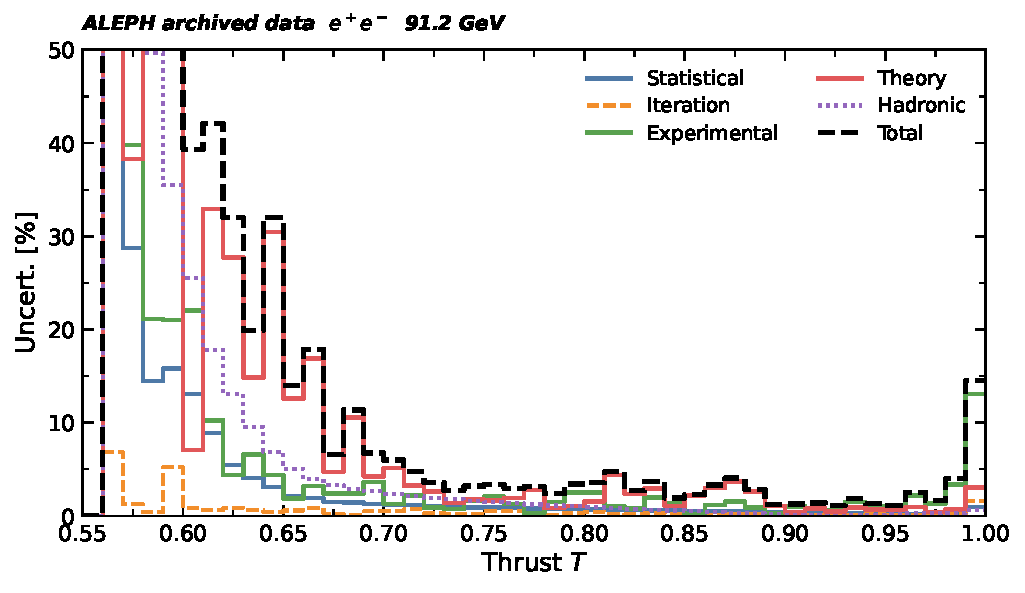
\includegraphics[width=0.72\textwidth]{../Studies/Phase2_Checks_2026-03-03/plots/uncertainty_breakdown/per_bin_uncertainty_grouped.pdf}
\caption{Per-bin absolute fractional uncertainty by group across the full measurement
range ($0.55\le T<1.0$): statistical, iteration envelope, experimental envelope,
theory envelope, hadronic correction, and total (dashed black). The $y$-axis is
limited to $50\%$.}
\label{fig:per_bin_uncertainty}
\end{figure}

\begin{figure}[t!]
\centering
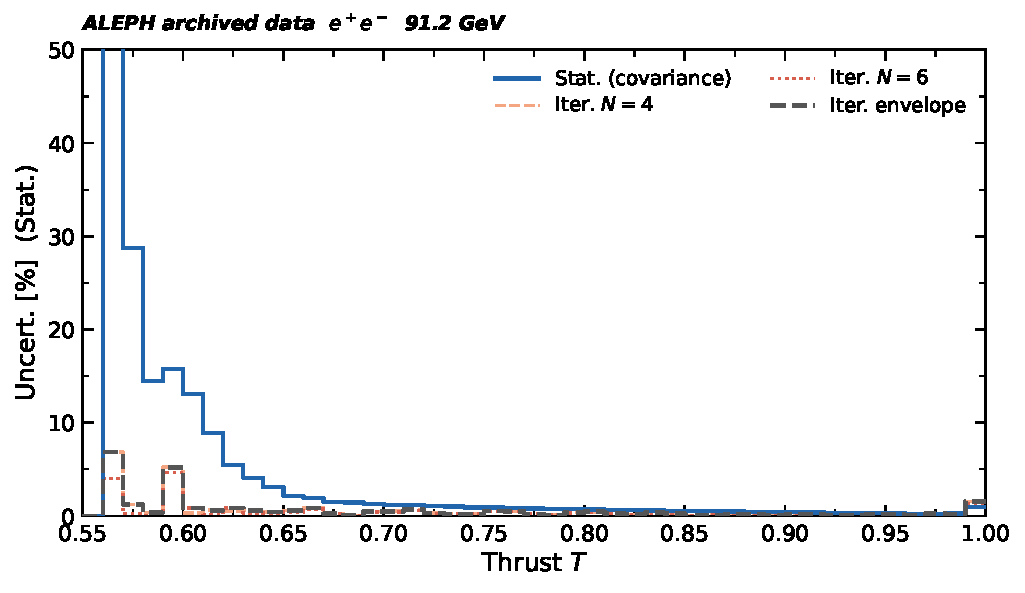
\includegraphics[width=0.72\textwidth]{../Studies/Phase2_Checks_2026-03-03/plots/uncertainty_breakdown/per_bin_uncertainty_stat.pdf}
\caption{Statistical and iteration-uncertainty breakdown. Dashed/dotted lines show
the signed variation for $N_{\mathrm{iter}}=4$ and $6$; the dashed-black line is the
iteration envelope. The $y$-axis is limited to $50\%$.}
\label{fig:per_bin_uncertainty_stat}
\end{figure}

\begin{figure}[t!]
\centering
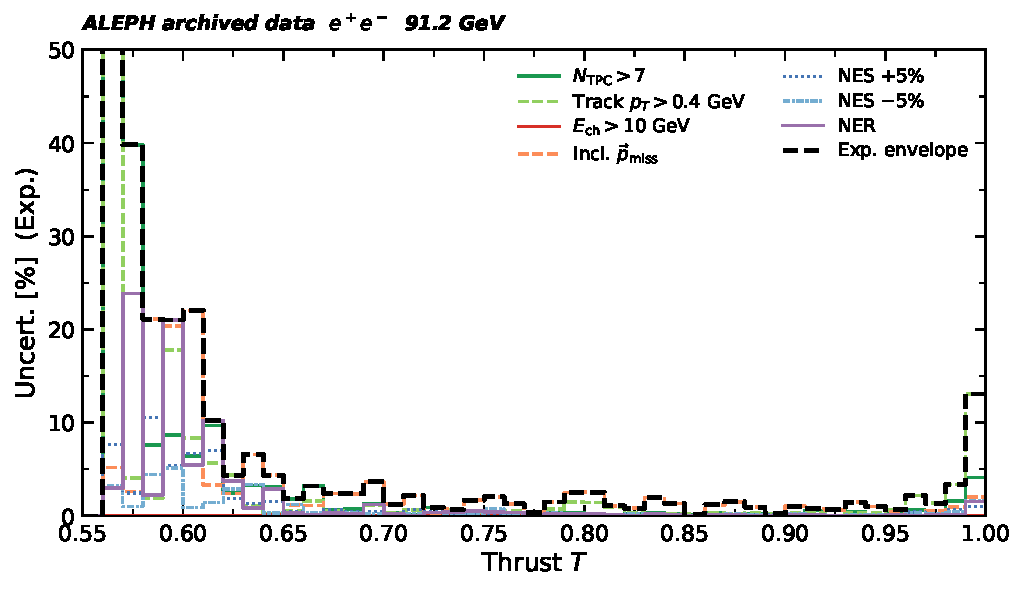
\includegraphics[width=0.72\textwidth]{../Studies/Phase2_Checks_2026-03-03/plots/uncertainty_breakdown/per_bin_uncertainty_exp.pdf}
\caption{Experimental uncertainty breakdown: seven individual variation branches
(track/event and neutral) with the group envelope (dashed black).
Large values at $T\lesssim 0.62$ arise because the nominal spectrum is steeply
rising from near zero there; even small absolute shifts produce large fractional
changes. The $y$-axis is limited to $50\%$.}
\label{fig:per_bin_uncertainty_exp}
\end{figure}

\begin{figure}[t!]
\centering
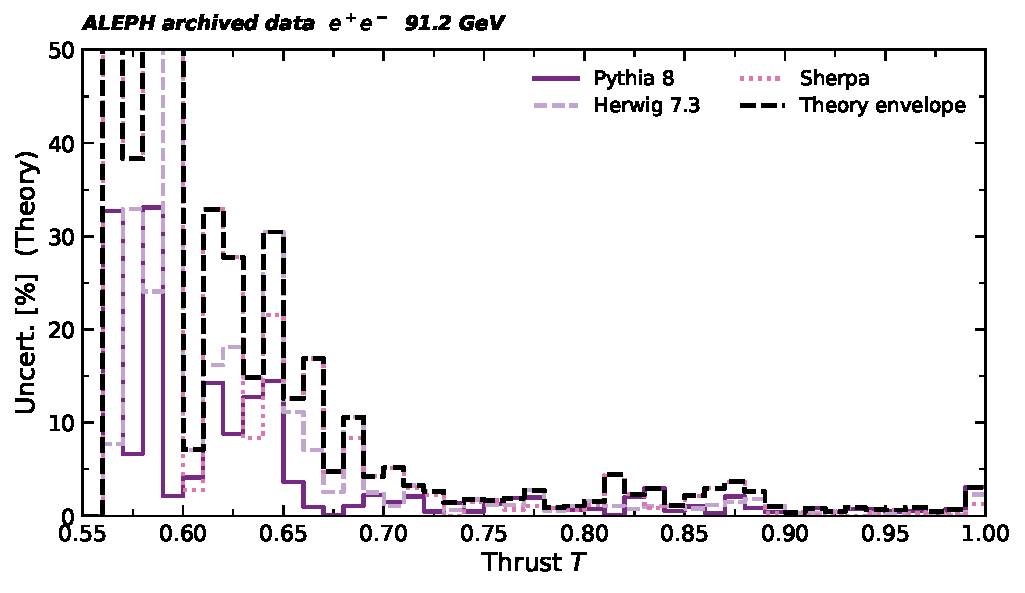
\includegraphics[width=0.72\textwidth]{../Studies/Phase2_Checks_2026-03-03/plots/uncertainty_breakdown/per_bin_uncertainty_theory.pdf}
\caption{Theory uncertainty breakdown: Pythia~8, Herwig~7.3, and Sherpa individual
shifts with the theory envelope (dashed black). The $y$-axis is limited to $50\%$.}
\label{fig:per_bin_uncertainty_theory}
\end{figure}

\begin{table}[t!]
\centering
\scriptsize
\begin{tabular}{c r c c c c c c}
\hline
$T$ range & $(1/\sigma)\,\mathrm{d}\sigma/\mathrm{d}T$ & Stat. & Iter. & Exp. & Theory & Had.\ corr. & Total \\
 & & [\%] & [\%] & [\%] & [\%] & [\%] & [\%] \\
\hline
[0.55,0.56) & \multicolumn{7}{c}{---} \\
{[0.56,0.57)} & $6.30\times10^{-5}$ & 88.8 & 6.9 & 467.8 & 67.7 & 139.7 & 500.9 \\
{[0.57,0.58)} & 0.0012 & 28.8 & 1.2 & 46.7 & 38.3 & 70.5 & 97.2 \\
{[0.58,0.59)} & 0.0015 & 14.5 & 0.4 & 25.0 & 59.5 & 49.6 & 82.7 \\
{[0.59,0.60)} & 0.0032 & 15.8 & 5.2 & 35.8 & 53.5 & 35.5 & 75.3 \\
{[0.60,0.61)} & 0.0042 & 13.1 & 0.9 & 25.9 & 7.1 & 25.5 & 39.3 \\
{[0.61,0.62)} & 0.0085 & 8.9 & 0.6 & 17.1 & 32.9 & 17.8 & 42.1 \\
{[0.62,0.63)} & 0.0131 & 5.5 & 0.9 & 7.3 & 27.7 & 13.0 & 32.0 \\
{[0.63,0.64)} & 0.0248 & 4.1 & 0.6 & 8.2 & 14.8 & 9.6 & 19.9 \\
{[0.64,0.65)} & 0.0411 & 3.1 & 0.5 & 6.3 & 30.5 & 6.9 & 32.0 \\
{[0.65,0.66)} & 0.0695 & 2.2 & 0.6 & 2.6 & 12.6 & 5.0 & 14.0 \\
{[0.66,0.67)} & 0.1068 & 1.9 & 0.8 & 3.8 & 16.9 & 3.9 & 17.9 \\
{[0.67,0.68)} & 0.1305 & 1.5 & 0.3 & 2.7 & 4.7 & 3.4 & 6.6 \\
{[0.68,0.69)} & 0.1587 & 1.5 & 0.1 & 2.6 & 10.6 & 2.9 & 11.4 \\
{[0.69,0.70)} & 0.1776 & 1.3 & 0.5 & 4.3 & 4.3 & 2.7 & 6.7 \\
{[0.70,0.71)} & 0.2087 & 1.2 & 0.5 & 1.4 & 5.2 & 2.4 & 6.0 \\
{[0.71,0.72)} & 0.2448 & 1.2 & 0.7 & 2.4 & 3.3 & 2.1 & 4.8 \\
{[0.72,0.73)} & 0.2876 & 1.0 & 0.3 & 1.1 & 2.6 & 1.9 & 3.6 \\
{[0.73,0.74)} & 0.3210 & 1.0 & 0.2 & 1.2 & 1.4 & 1.8 & 2.8 \\
{[0.74,0.75)} & 0.3792 & 0.9 & 0.2 & 1.9 & 1.8 & 1.6 & 3.2 \\
{[0.75,0.76)} & 0.4332 & 0.9 & 0.6 & 2.3 & 1.7 & 1.5 & 3.4 \\
{[0.76,0.77)} & 0.4958 & 0.8 & 0.5 & 1.5 & 1.9 & 1.4 & 3.0 \\
{[0.77,0.78)} & 0.5504 & 0.8 & 0.2 & 0.5 & 2.8 & 1.2 & 3.2 \\
{[0.78,0.79)} & 0.5994 & 0.7 & 0.1 & 1.8 & 0.9 & 1.1 & 2.4 \\
{[0.79,0.80)} & 0.6550 & 0.8 & 0.4 & 3.0 & 1.1 & 1.0 & 3.4 \\
{[0.80,0.81)} & 0.7399 & 0.7 & 0.5 & 3.0 & 1.6 & 0.9 & 3.6 \\
{[0.81,0.82)} & 0.8395 & 0.7 & 0.3 & 1.4 & 4.4 & 0.8 & 4.8 \\
{[0.82,0.83)} & 0.9697 & 0.6 & 0.2 & 0.9 & 2.3 & 0.8 & 2.7 \\
{[0.83,0.84)} & 1.14 & 0.6 & 0.3 & 2.0 & 3.0 & 0.7 & 3.7 \\
{[0.84,0.85)} & 1.26 & 0.6 & 0.3 & 1.4 & 1.1 & 0.6 & 1.9 \\
{[0.85,0.86)} & 1.45 & 0.5 & 0.0 & 0.3 & 2.2 & 0.5 & 2.3 \\
{[0.86,0.87)} & 1.64 & 0.5 & 0.1 & 1.3 & 3.0 & 0.4 & 3.3 \\
{[0.87,0.88)} & 1.89 & 0.5 & 0.2 & 1.6 & 3.7 & 0.4 & 4.1 \\
{[0.88,0.89)} & 2.23 & 0.5 & 0.2 & 1.0 & 2.6 & 0.3 & 2.9 \\
{[0.89,0.90)} & 2.67 & 0.4 & 0.1 & 0.4 & 1.0 & 0.2 & 1.2 \\
{[0.90,0.91)} & 3.20 & 0.4 & 0.1 & 1.2 & 0.4 & 0.1 & 1.3 \\
{[0.91,0.92)} & 3.86 & 0.4 & 0.2 & 1.1 & 0.8 & 0.1 & 1.4 \\
{[0.92,0.93)} & 4.70 & 0.4 & 0.1 & 0.9 & 0.5 & 0.0 & 1.1 \\
{[0.93,0.94)} & 5.79 & 0.3 & 0.1 & 1.6 & 0.9 & 0.1 & 1.9 \\
{[0.94,0.95)} & 7.40 & 0.3 & 0.2 & 1.1 & 0.7 & 0.1 & 1.4 \\
{[0.95,0.96)} & 9.79 & 0.3 & 0.1 & 0.8 & 0.6 & 0.2 & 1.1 \\
{[0.96,0.97)} & 13.86 & 0.2 & 0.1 & 2.3 & 1.0 & 0.3 & 2.5 \\
{[0.97,0.98)} & 18.46 & 0.2 & 0.3 & 1.5 & 0.5 & 0.4 & 1.6 \\
{[0.98,0.99)} & 12.18 & 0.3 & 0.2 & 3.9 & 0.7 & 0.3 & 4.0 \\
{[0.99,1.00)} & 1.01 & 1.0 & 1.6 & 14.1 & 3.1 & 0.7 & 14.5 \\
\hline
\end{tabular}
\normalsize
\caption{Per-bin fractional uncertainties across the full measurement range ($0.55 \leq T < 1.0$). The second column gives the nominal unfolded $(1/\sigma)\,\mathrm{d}\sigma/\mathrm{d}T$ value; all remaining columns are absolute fractional uncertainties in percent. Bins with zero nominal spectrum (dashes) are below threshold. \textit{Exp.} denotes the total experimental component (track/event and neutral sub-components combined in quadrature), and \textit{Had.\ corr.} denotes the hadronic event-selection correction uncertainty.}
\label{tab:per_bin_uncertainty}
\end{table}

\begin{table}[t!]
\centering
\scriptsize
\begin{tabular}{c r r r r}
\hline
$T$ range & Our $(1/\sigma)\,\mathrm{d}\sigma/\mathrm{d}T$ & Our total unc.\ [\%] & ALEPH 2004 $(1/\sigma)\,\mathrm{d}\sigma/\mathrm{d}T$ & ALEPH 2004 total unc.\ [\%] \\
\hline
[0.55,0.56) & \multicolumn{1}{c}{---} & \multicolumn{1}{c}{---} & \multicolumn{1}{c}{---} & \multicolumn{1}{c}{---} \\
{[0.56,0.57)} & $6.30\times10^{-5}$ & 500.9 & \multicolumn{1}{c}{---} & \multicolumn{1}{c}{---} \\
{[0.57,0.58)} & 0.0012 & 97.2 & \multicolumn{1}{c}{---} & \multicolumn{1}{c}{---} \\
{[0.58,0.59)} & 0.0015 & 82.7 & 0.0011 & 61.2 \\
{[0.59,0.60)} & 0.0032 & 75.3 & 0.0023 & 54.1 \\
{[0.60,0.61)} & 0.0042 & 39.3 & 0.0035 & 41.7 \\
{[0.61,0.62)} & 0.0085 & 42.1 & 0.0084 & 25.0 \\
{[0.62,0.63)} & 0.0131 & 32.0 & 0.0128 & 23.1 \\
{[0.63,0.64)} & 0.0248 & 19.9 & 0.0215 & 21.9 \\
{[0.64,0.65)} & 0.0411 & 32.0 & 0.0433 & 14.4 \\
{[0.65,0.66)} & 0.0695 & 14.0 & 0.0656 & 9.2 \\
{[0.66,0.67)} & 0.1068 & 17.9 & 0.1028 & 8.5 \\
{[0.67,0.68)} & 0.1305 & 6.6 & 0.1258 & 8.7 \\
{[0.68,0.69)} & 0.1587 & 11.4 & 0.1640 & 8.7 \\
{[0.69,0.70)} & 0.1776 & 6.7 & 0.1842 & 9.5 \\
{[0.70,0.71)} & 0.2087 & 6.0 & 0.2142 & 7.6 \\
{[0.71,0.72)} & 0.2448 & 4.8 & 0.2481 & 9.1 \\
{[0.72,0.73)} & 0.2876 & 3.6 & 0.2943 & 7.5 \\
{[0.73,0.74)} & 0.3210 & 2.8 & 0.3435 & 6.2 \\
{[0.74,0.75)} & 0.3792 & 3.2 & 0.3654 & 6.0 \\
{[0.75,0.76)} & 0.4332 & 3.4 & 0.4309 & 6.0 \\
{[0.76,0.77)} & 0.4958 & 3.0 & 0.4692 & 4.9 \\
{[0.77,0.78)} & 0.5504 & 3.2 & 0.5458 & 4.2 \\
{[0.78,0.79)} & 0.5994 & 2.4 & 0.5994 & 4.2 \\
{[0.79,0.80)} & 0.6550 & 3.4 & 0.6609 & 5.6 \\
{[0.80,0.81)} & 0.7399 & 3.6 & 0.7680 & 4.6 \\
{[0.81,0.82)} & 0.8395 & 4.8 & 0.8570 & 4.3 \\
{[0.82,0.83)} & 0.9697 & 2.7 & 0.9808 & 5.1 \\
{[0.83,0.84)} & 1.14 & 3.7 & 1.11 & 5.0 \\
{[0.84,0.85)} & 1.26 & 1.9 & 1.27 & 4.9 \\
{[0.85,0.86)} & 1.45 & 2.3 & 1.44 & 3.8 \\
{[0.86,0.87)} & 1.64 & 3.3 & 1.64 & 4.0 \\
{[0.87,0.88)} & 1.89 & 4.1 & 1.93 & 3.9 \\
{[0.88,0.89)} & 2.23 & 2.9 & 2.23 & 3.4 \\
{[0.89,0.90)} & 2.67 & 1.2 & 2.63 & 3.2 \\
{[0.90,0.91)} & 3.20 & 1.3 & 3.06 & 3.3 \\
{[0.91,0.92)} & 3.86 & 1.4 & 3.70 & 2.2 \\
{[0.92,0.93)} & 4.70 & 1.1 & 4.55 & 2.3 \\
{[0.93,0.94)} & 5.79 & 1.9 & 5.64 & 2.2 \\
{[0.94,0.95)} & 7.40 & 1.4 & 7.28 & 1.7 \\
{[0.95,0.96)} & 9.79 & 1.1 & 9.63 & 1.7 \\
{[0.96,0.97)} & 13.86 & 2.5 & 13.60 & 1.7 \\
{[0.97,0.98)} & 18.46 & 1.6 & 18.57 & 3.7 \\
{[0.98,0.99)} & 12.18 & 4.0 & 12.89 & 4.1 \\
{[0.99,1.00)} & 1.01 & 14.5 & 1.31 & 15.4 \\
\hline
\end{tabular}
\normalsize
\caption{Comparison of the nominal unfolded $(1/\sigma)\,\mathrm{d}\sigma/\mathrm{d}T$ and total fractional uncertainty with the published ALEPH 2004 result (HEPData ins:636645, Table~54) across the full measurement range ($0.55\le T<1.0$). The ALEPH 2004 total uncertainty combines statistical, sys$_1$, and sys$_2$ components in quadrature. Dashes indicate bins not covered by one or both measurements.}
\label{tab:per_bin_uncertainty_aleph}
\end{table}

\begin{table}[t!]
\centering
\scriptsize
\resizebox{\textwidth}{!}{%
\begin{tabular}{c  r r r r  r r r r  r r}
\hline
& \multicolumn{2}{c}{$(1/\sigma)\,\mathrm{d}\sigma/\mathrm{d}T$}
 & \multicolumn{2}{c}{Stat.\ [\%]}
 & \multicolumn{2}{c}{Exp.\ / Sys.\,1 [\%]}
 & \multicolumn{2}{c}{Theory\,/ Sys.\,2 [\%]}
 & \multicolumn{2}{c}{Total [\%]} \\
\cline{2-3}\cline{4-5}\cline{6-7}\cline{8-9}\cline{10-11}
$T$ range & Ours & ALEPH & Ours & ALEPH & Ours & ALEPH & Ours & ALEPH & Ours & ALEPH \\
\hline
{[0.55,0.56)} & \multicolumn{10}{c}{---} \\
{[0.56,0.57)} & $6.30{\times}10^{-5}$ & --- & 88.8 & --- & 467.8 & --- & 67.7 & --- & 500.9 & --- \\
{[0.57,0.58)} & $1.22{\times}10^{-3}$ & --- & 28.8 & --- & 46.7 & --- & 38.3 & --- & 97.2 & --- \\
{[0.58,0.59)} & $1.48{\times}10^{-3}$ & $1.15{\times}10^{-3}$ & 14.5 & 29.6 & 25.0 & 45.2 & 59.5 & 28.7 & 82.7 & 61.2 \\
{[0.59,0.60)} & $3.23{\times}10^{-3}$ & $2.29{\times}10^{-3}$ & 15.8 & 21.8 & 35.8 & 40.6 & 53.5 & 28.4 & 75.3 & 54.1 \\
{[0.60,0.61)} & $4.20{\times}10^{-3}$ & $3.50{\times}10^{-3}$ & 13.1 & 17.4 & 25.9 & 24.9 & 7.1 & 28.6 & 39.3 & 41.7 \\
{[0.61,0.62)} & $8.53{\times}10^{-3}$ & $8.39{\times}10^{-3}$ & 8.9 & 11.4 & 17.1 & 9.2 & 32.9 & 20.3 & 42.1 & 25.0 \\
{[0.62,0.63)} & 0.0131 & 0.0128 & 5.5 & 9.0 & 7.3 & 6.4 & 27.7 & 20.3 & 32.0 & 23.1 \\
{[0.63,0.64)} & 0.0248 & 0.0215 & 4.1 & 7.1 & 8.2 & 4.4 & 14.8 & 20.3 & 19.9 & 21.9 \\
{[0.64,0.65)} & 0.0411 & 0.0433 & 3.1 & 5.2 & 6.3 & 11.5 & 30.5 & 7.1 & 32.0 & 14.4 \\
{[0.65,0.66)} & 0.0695 & 0.0656 & 2.2 & 4.1 & 2.6 & 4.2 & 12.6 & 7.1 & 14.0 & 9.2 \\
{[0.66,0.67)} & 0.1068 & 0.1028 & 1.9 & 3.2 & 3.8 & 3.4 & 16.9 & 7.1 & 17.9 & 8.5 \\
{[0.67,0.68)} & 0.1305 & 0.1258 & 1.5 & 2.9 & 2.7 & 2.4 & 4.7 & 7.8 & 6.6 & 8.7 \\
{[0.68,0.69)} & 0.1587 & 0.1640 & 1.5 & 2.5 & 2.6 & 2.9 & 10.6 & 7.8 & 11.4 & 8.7 \\
{[0.69,0.70)} & 0.1776 & 0.1842 & 1.3 & 2.4 & 4.3 & 4.7 & 4.3 & 7.8 & 6.7 & 9.5 \\
{[0.70,0.71)} & 0.2087 & 0.2142 & 1.2 & 2.2 & 1.4 & 2.1 & 5.2 & 7.0 & 6.0 & 7.6 \\
{[0.71,0.72)} & 0.2448 & 0.2481 & 1.2 & 2.1 & 2.4 & 5.4 & 3.3 & 7.0 & 4.8 & 9.1 \\
{[0.72,0.73)} & 0.2876 & 0.2943 & 1.0 & 1.9 & 1.1 & 1.9 & 2.6 & 7.0 & 3.6 & 7.5 \\
{[0.73,0.74)} & 0.3210 & 0.3435 & 1.0 & 1.8 & 1.2 & 2.3 & 1.4 & 5.5 & 2.8 & 6.2 \\
{[0.74,0.75)} & 0.3792 & 0.3654 & 0.9 & 1.7 & 1.9 & 1.9 & 1.8 & 5.5 & 3.2 & 6.0 \\
{[0.75,0.76)} & 0.4332 & 0.4309 & 0.9 & 1.6 & 2.3 & 2.0 & 1.7 & 5.5 & 3.4 & 6.0 \\
{[0.76,0.77)} & 0.4958 & 0.4692 & 0.8 & 1.5 & 1.5 & 2.8 & 1.9 & 3.7 & 3.0 & 4.9 \\
{[0.77,0.78)} & 0.5504 & 0.5458 & 0.8 & 1.4 & 0.5 & 1.3 & 2.8 & 3.7 & 3.2 & 4.2 \\
{[0.78,0.79)} & 0.5994 & 0.5994 & 0.7 & 1.4 & 1.8 & 1.3 & 0.9 & 3.7 & 2.4 & 4.2 \\
{[0.79,0.80)} & 0.6550 & 0.6609 & 0.8 & 1.3 & 3.0 & 3.7 & 1.1 & 3.9 & 3.4 & 5.6 \\
{[0.80,0.81)} & 0.7399 & 0.7680 & 0.7 & 1.2 & 3.0 & 2.0 & 1.6 & 3.9 & 3.6 & 4.6 \\
{[0.81,0.82)} & 0.8395 & 0.8570 & 0.7 & 1.1 & 1.4 & 1.4 & 4.4 & 3.9 & 4.8 & 4.3 \\
{[0.82,0.83)} & 0.9697 & 0.9808 & 0.6 & 1.1 & 0.9 & 1.3 & 2.3 & 4.8 & 2.7 & 5.1 \\
{[0.83,0.84)} & 1.14 & 1.11 & 0.6 & 1.0 & 2.0 & 0.8 & 3.0 & 4.8 & 3.7 & 5.0 \\
{[0.84,0.85)} & 1.26 & 1.27 & 0.6 & 1.0 & 1.4 & 0.7 & 1.1 & 4.8 & 1.9 & 4.9 \\
{[0.85,0.86)} & 1.45 & 1.44 & 0.5 & 0.9 & 0.3 & 0.7 & 2.2 & 3.6 & 2.3 & 3.8 \\
{[0.86,0.87)} & 1.64 & 1.64 & 0.5 & 0.8 & 1.3 & 1.5 & 3.0 & 3.6 & 3.3 & 4.0 \\
{[0.87,0.88)} & 1.89 & 1.93 & 0.5 & 0.8 & 1.6 & 1.3 & 3.7 & 3.6 & 4.1 & 3.9 \\
{[0.88,0.89)} & 2.23 & 2.23 & 0.5 & 0.7 & 1.0 & 1.3 & 2.6 & 3.1 & 2.9 & 3.4 \\
{[0.89,0.90)} & 2.67 & 2.63 & 0.4 & 0.7 & 0.4 & 0.6 & 1.0 & 3.1 & 1.2 & 3.2 \\
{[0.90,0.91)} & 3.20 & 3.06 & 0.4 & 0.6 & 1.2 & 1.1 & 0.4 & 3.1 & 1.3 & 3.3 \\
{[0.91,0.92)} & 3.86 & 3.70 & 0.4 & 0.6 & 1.1 & 0.6 & 0.8 & 2.1 & 1.4 & 2.2 \\
{[0.92,0.93)} & 4.70 & 4.55 & 0.4 & 0.5 & 0.9 & 0.8 & 0.5 & 2.1 & 1.1 & 2.3 \\
{[0.93,0.94)} & 5.79 & 5.64 & 0.3 & 0.5 & 1.6 & 0.7 & 0.9 & 2.1 & 1.9 & 2.2 \\
{[0.94,0.95)} & 7.40 & 7.28 & 0.3 & 0.4 & 1.1 & 0.6 & 0.7 & 1.5 & 1.4 & 1.7 \\
{[0.95,0.96)} & 9.79 & 9.63 & 0.3 & 0.4 & 0.8 & 0.7 & 0.6 & 1.5 & 1.1 & 1.7 \\
{[0.96,0.97)} & 13.9 & 13.6 & 0.2 & 0.3 & 2.3 & 0.6 & 1.0 & 1.5 & 2.5 & 1.7 \\
{[0.97,0.98)} & 18.5 & 18.6 & 0.2 & 0.3 & 1.5 & 0.5 & 0.5 & 3.7 & 1.6 & 3.7 \\
{[0.98,0.99)} & 12.2 & 12.9 & 0.3 & 0.3 & 3.9 & 1.8 & 0.7 & 3.7 & 4.0 & 4.1 \\
{[0.99,1.00)} & 1.01 & 1.31 & 1.0 & 0.8 & 14.1 & 14.9 & 3.1 & 3.7 & 14.5 & 15.4 \\
\hline
\end{tabular}
}% end resizebox
\normalsize
\caption{Per-bin fractional uncertainty breakdown comparison between this analysis and the published ALEPH 2004 result (HEPData ins:636645, Table~54). For this analysis, Stat.\ is derived from the RooUnfold covariance, Exp.\ is the quadrature sum of all experimental track/event and neutral variations, and Theory is the max envelope of the three generator reweightings. For ALEPH 2004, Sys.\,1 and Sys.\,2 correspond to the two systematic components provided in the HEPData table. All values are absolute fractional uncertainties in percent; Total combines all components in quadrature. Dashes indicate bins outside the respective measurement range.}
\label{tab:per_bin_uncertainty_breakdown_comparison}
\end{table}


\subsection{Uncertainty structure across components}

\begin{figure}[t!]
\centering
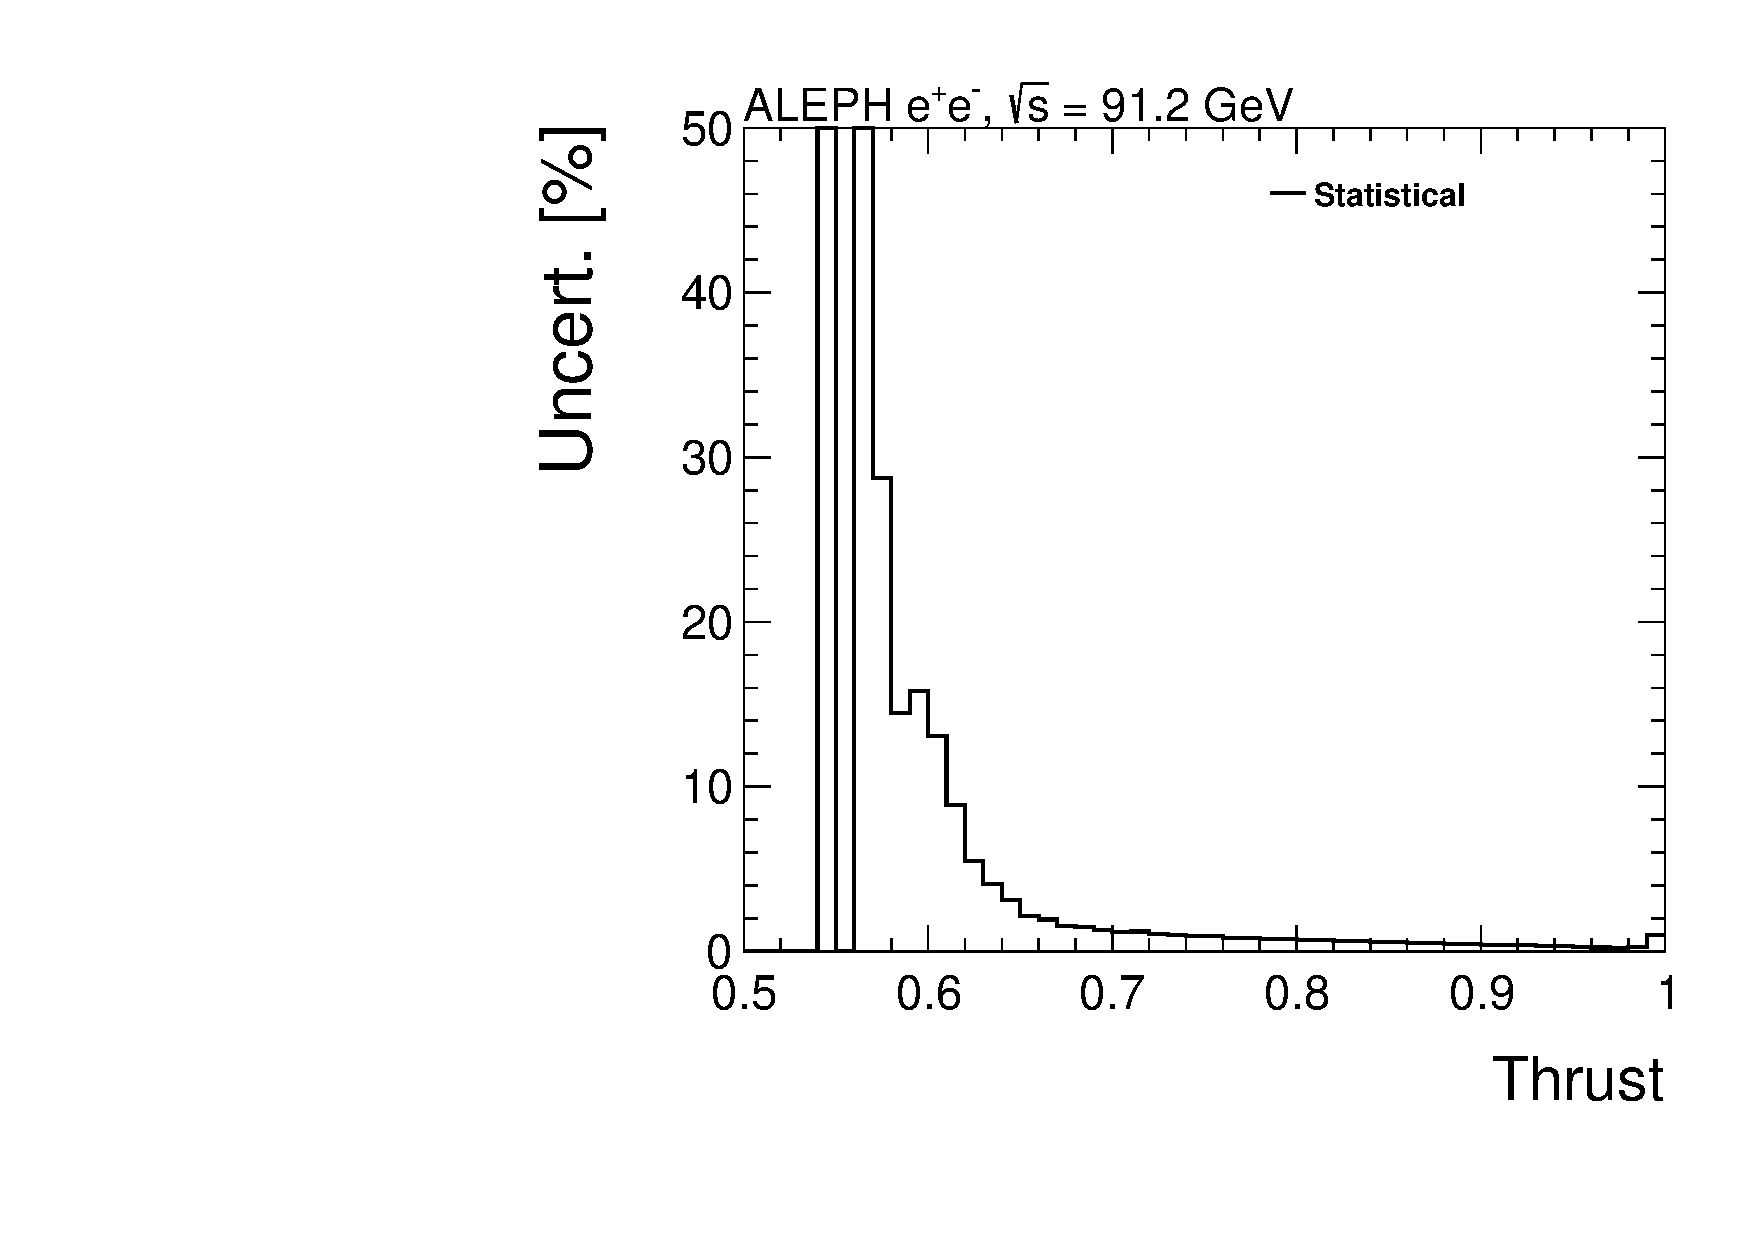
\includegraphics[width=0.49\textwidth]{../Studies/PreliminaryResult/2026-02-17_thrust_iter5/summary/uncertainty_components_statistical.pdf}
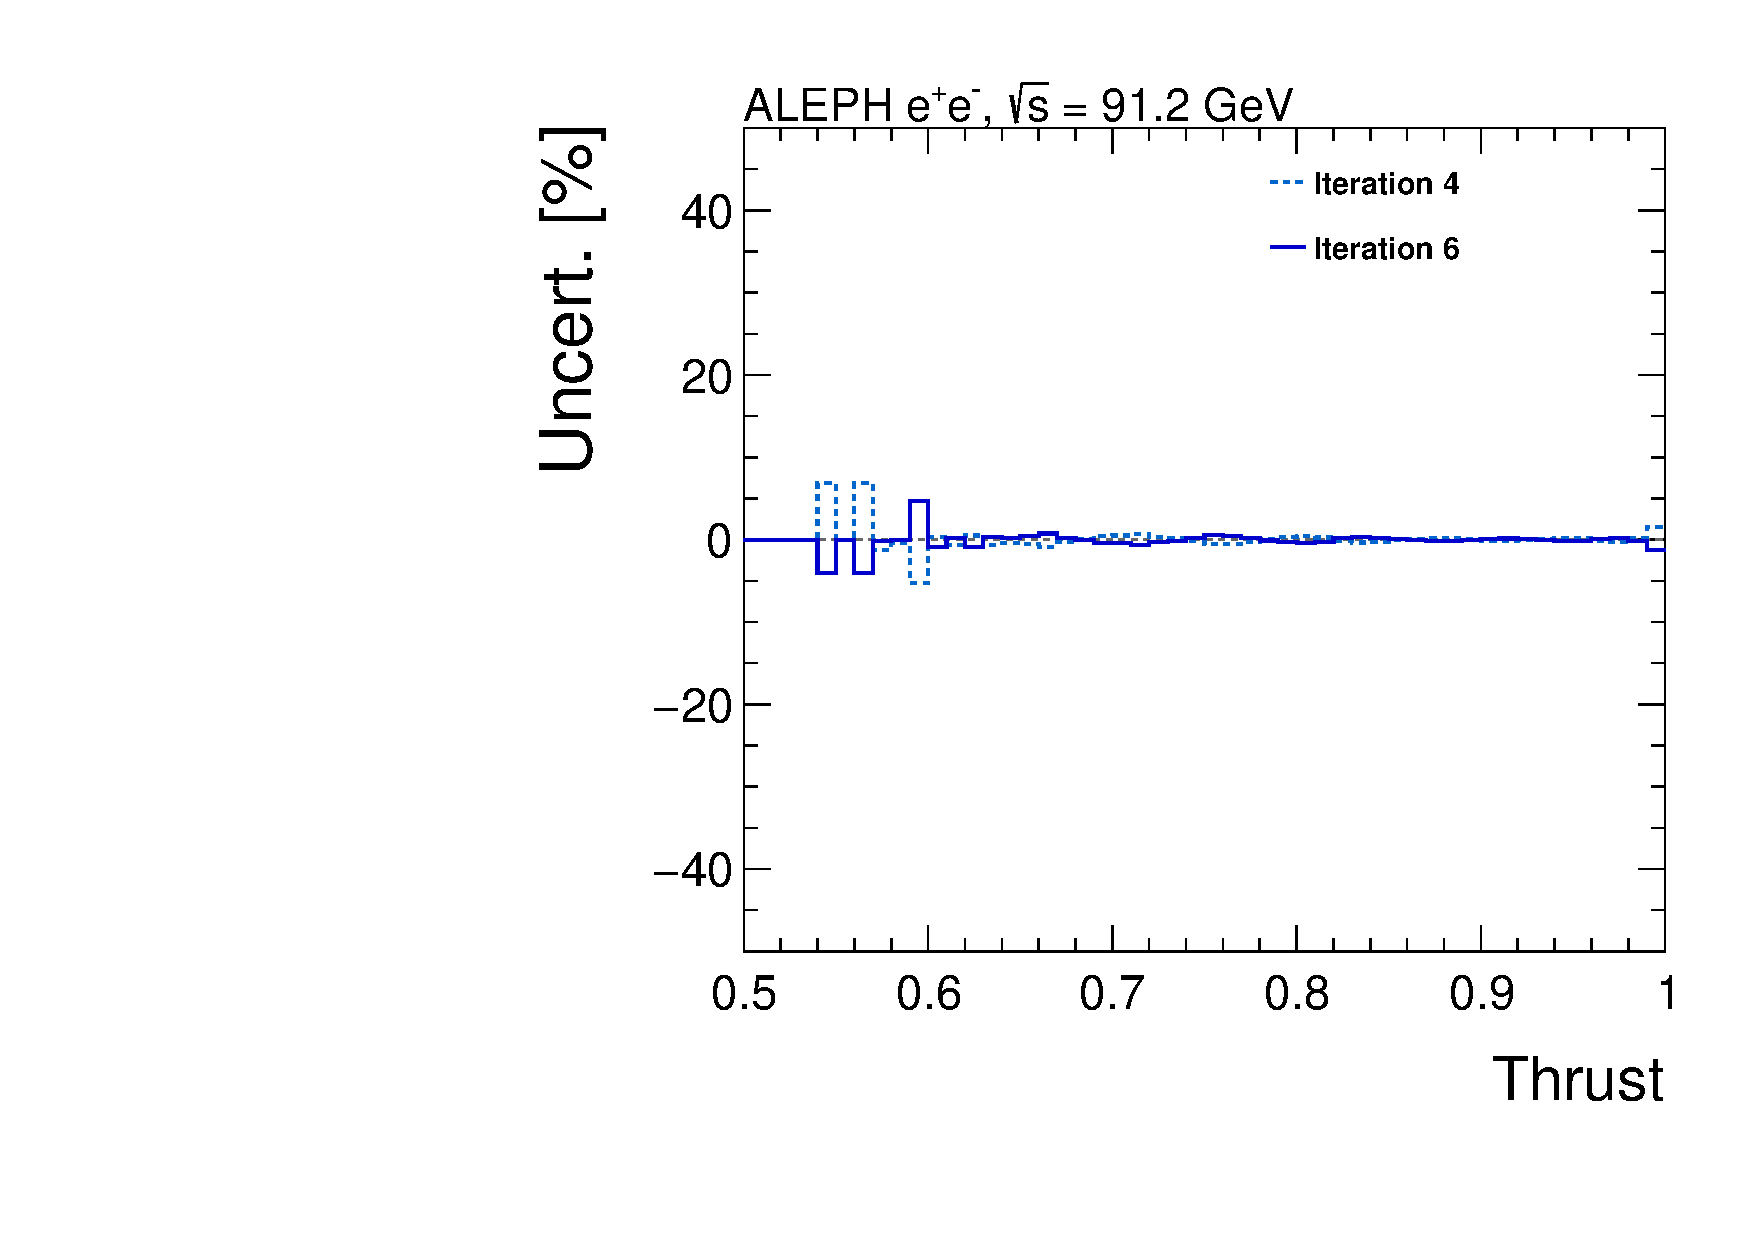
\includegraphics[width=0.49\textwidth]{../Studies/PreliminaryResult/2026-02-17_thrust_iter5/summary/uncertainty_components_unfolding.pdf}
\\
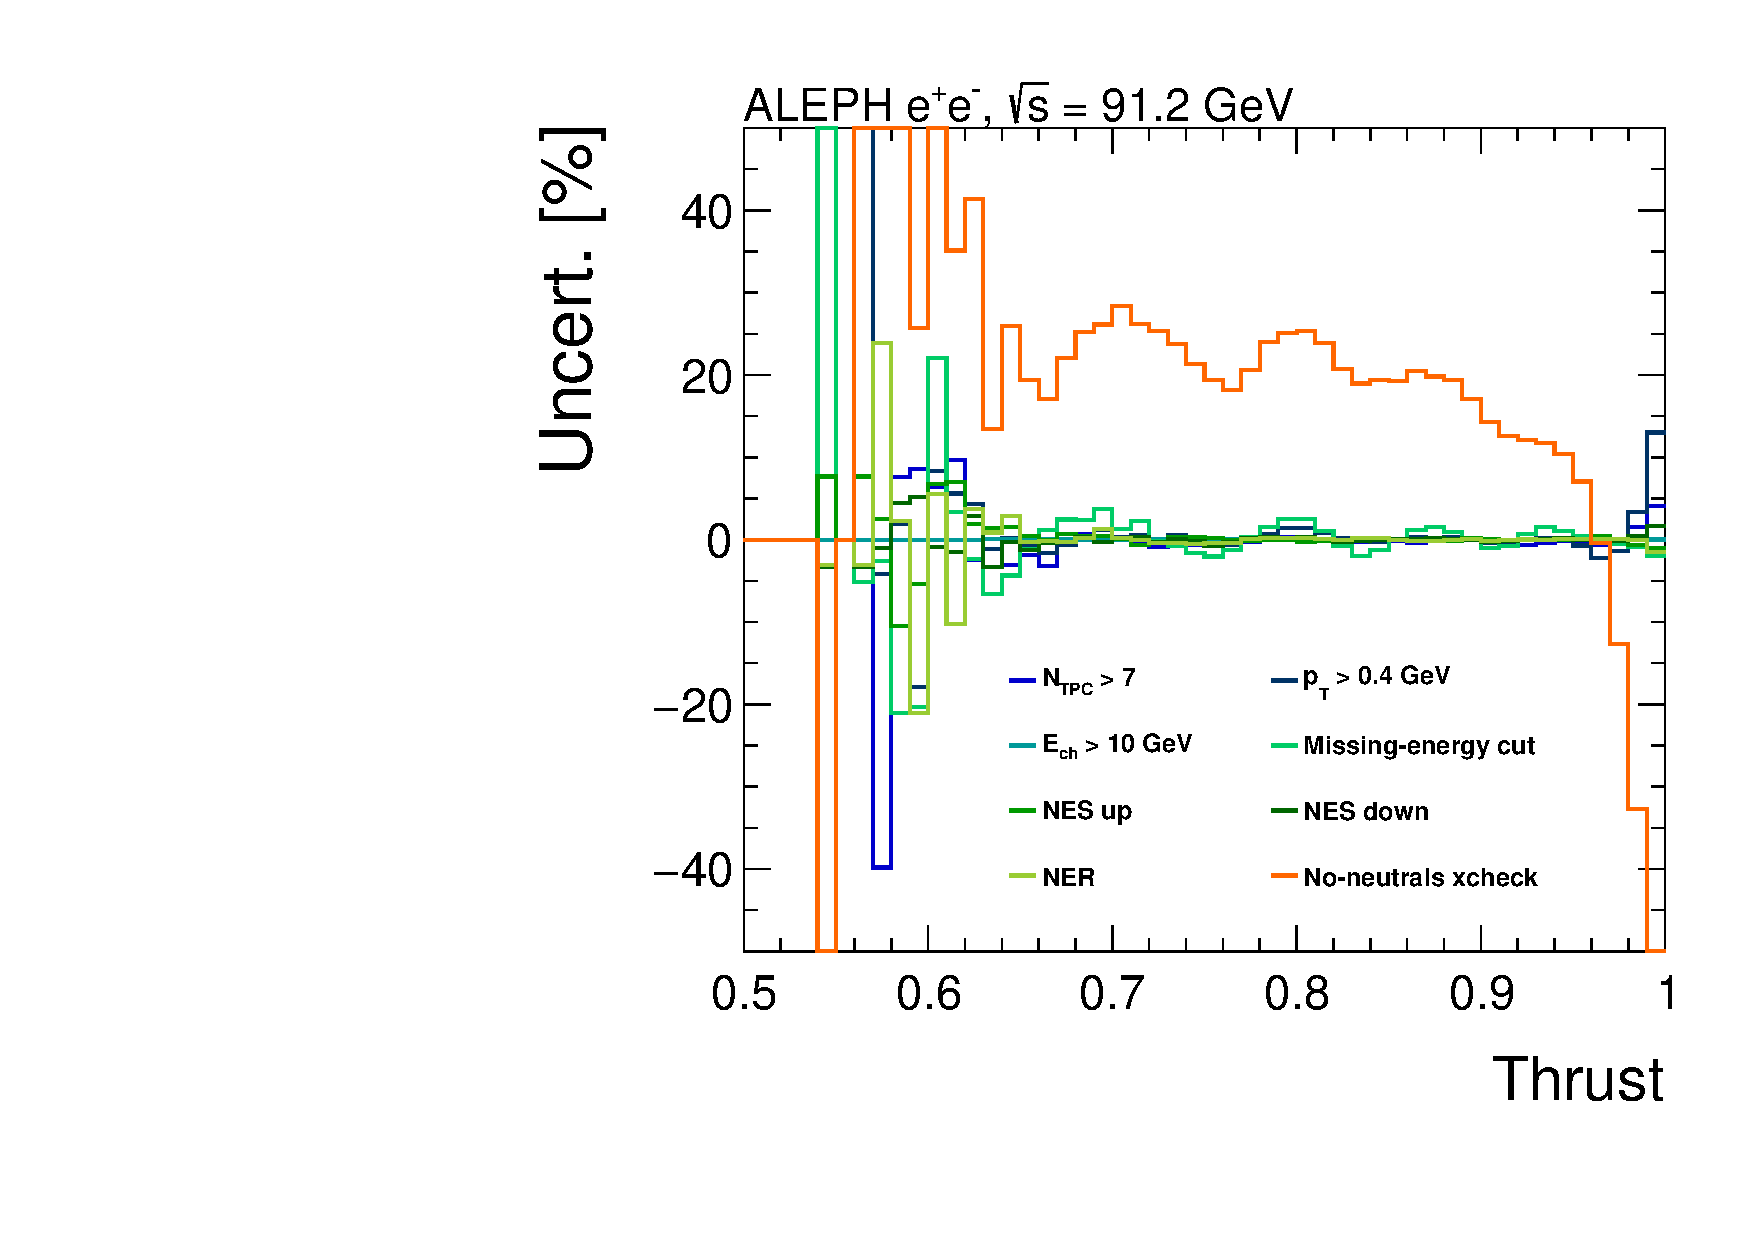
\includegraphics[width=0.49\textwidth]{../Studies/PreliminaryResult/2026-02-17_thrust_iter5/summary/uncertainty_components_experimental.pdf}
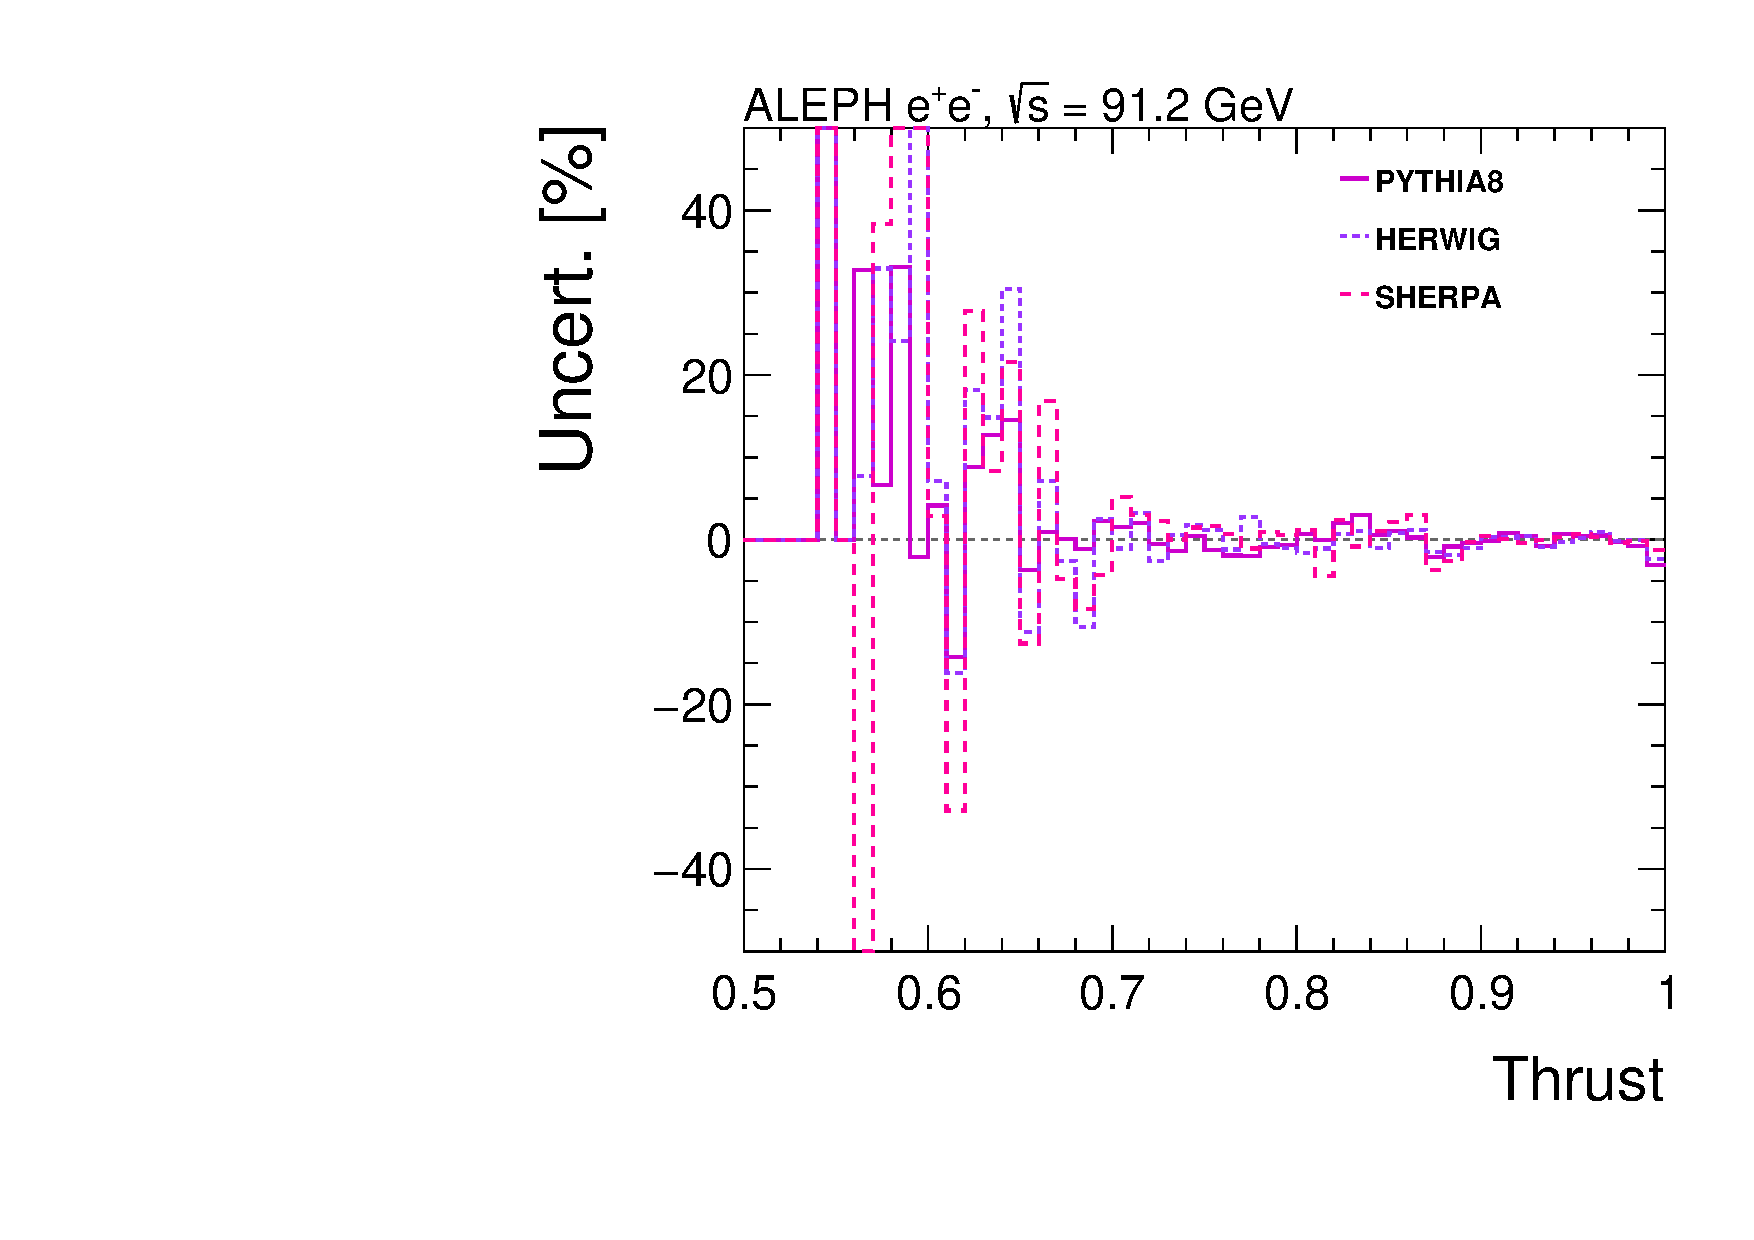
\includegraphics[width=0.49\textwidth]{../Studies/PreliminaryResult/2026-02-17_thrust_iter5/summary/uncertainty_components_theory.pdf}
\caption{Uncertainty components in four views: statistical (top left), unfolding iterations (top right), experimental variations (bottom left), and theory reweighting (bottom right). Non-statistical panels show signed shifts relative to nominal in percent; displayed $y$-ranges are clipped to $\pm 50\%$ for readability.}
\label{fig:uncertainty_components_fourpanel}
\end{figure}

The dominant mean contributions in the central range ($0.60\le T<0.95$) are theory
and experimental components, while the iteration uncertainty is subleading for the
nominal regularization choice. The hadronic correction uncertainty is an additional
independent component. The mean total uncertainty in the central range is $8.43\%$,
dominated by the theory envelope; this figure is derived from the diagonal of the
total covariance matrix in the differential cross-section basis.

\subsection{Final total correlation matrix}

\begin{figure}[t!]
\centering
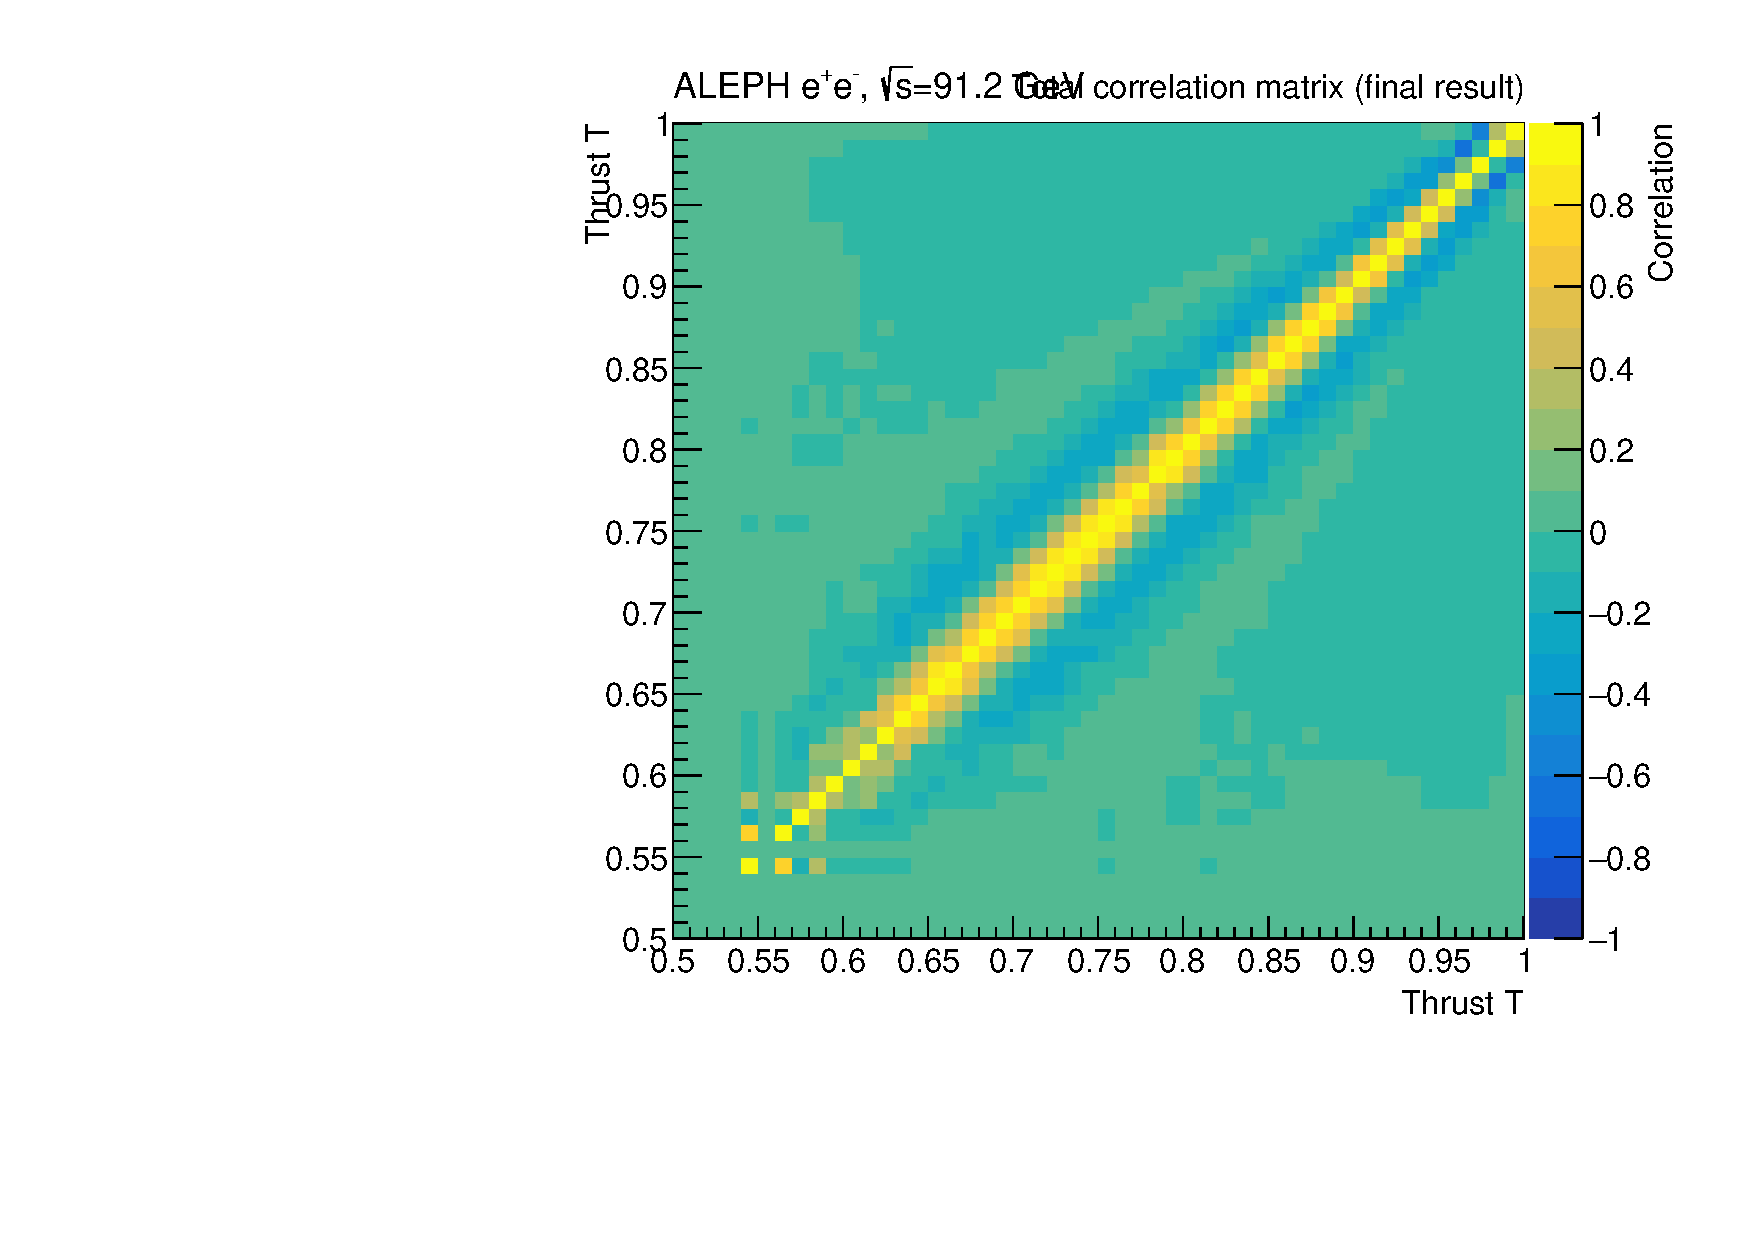
\includegraphics[width=0.82\textwidth]{../Studies/PreliminaryResult/2026-02-17_thrust_iter5/summary/matrix_total_correlation_final.pdf}
\caption{Total bin-to-bin correlation matrix for the final result, combining statistical, unfolding-iteration, experimental, theory, and hadronic-correction components using the \texttt{template\_correlated} covariance model.}
\label{fig:final_total_correlation_matrix}
\end{figure}

Figure~\ref{fig:final_total_correlation_matrix} shows the total correlation structure.
The matrix is non-diagonal, with largest off-diagonal correlation $|\rho_{ij}|=0.889$,
confirming that correlated information is preserved in the exported products intended
for downstream phenomenology.

\subsection{Final unfolded thrust distribution}

\begin{figure}[h!]
\centering
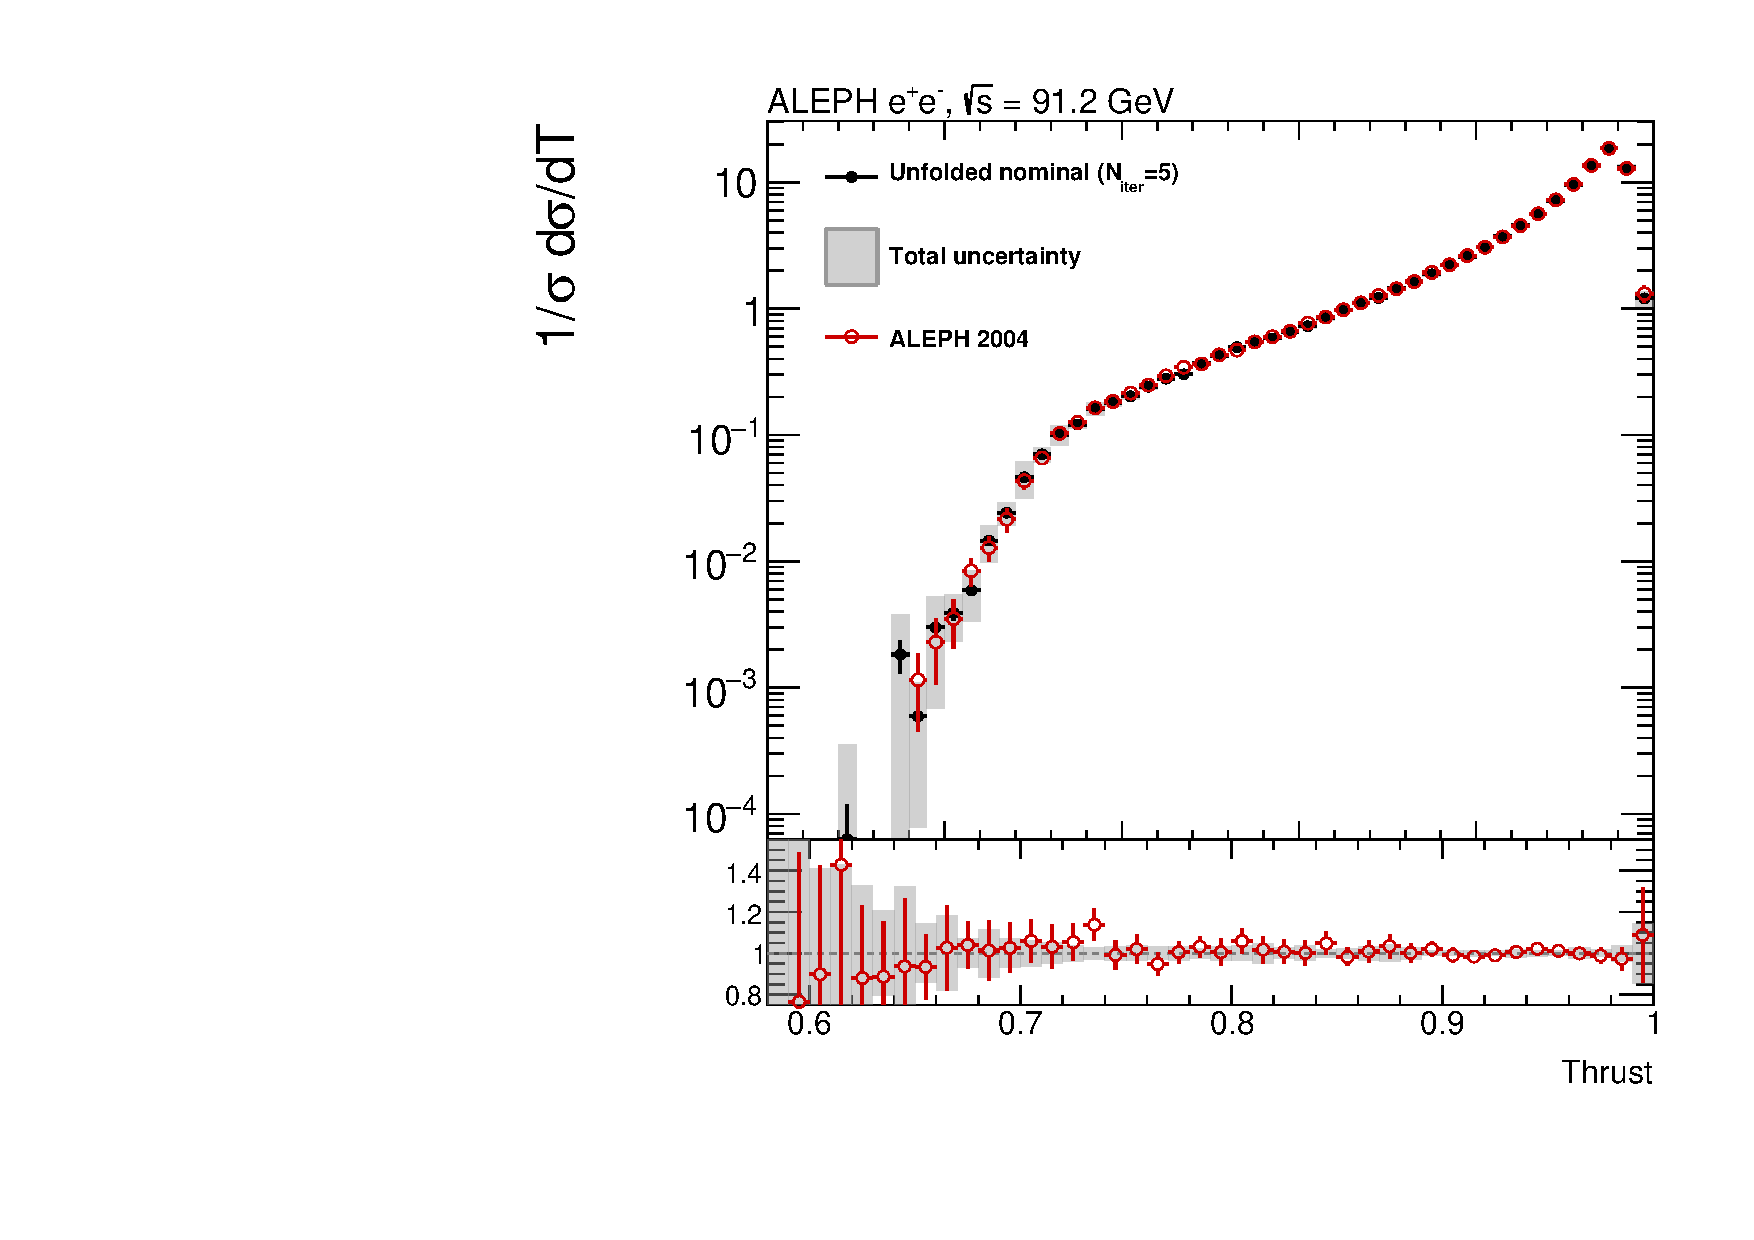
\includegraphics[width=0.48\textwidth]{../Studies/PreliminaryResult/2026-02-17_thrust_iter5/summary/final_result_uncertainty_breakdown.pdf}%
\hfill%
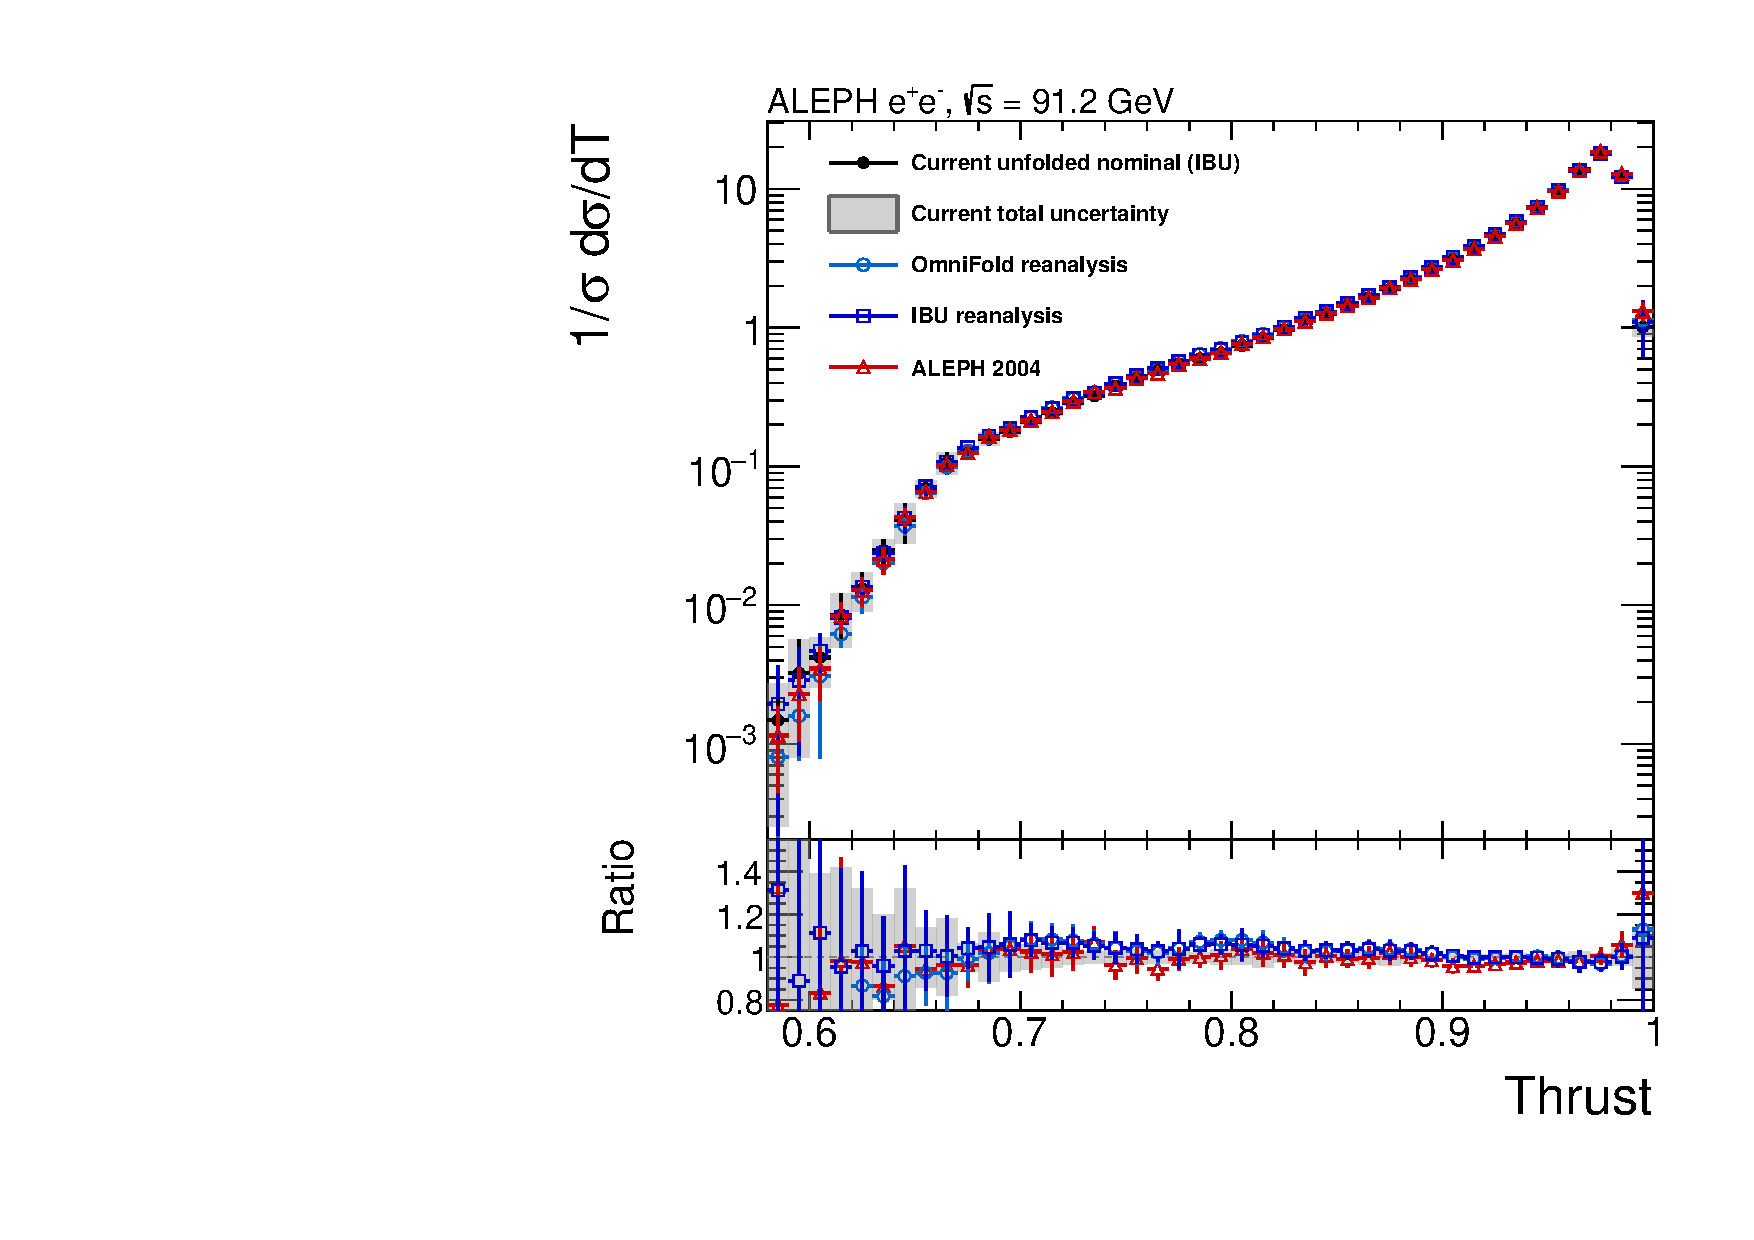
\includegraphics[width=0.48\textwidth]{../Studies/PreliminaryResult/2026-02-17_thrust_iter5/summary/final_result_of_ibu_comparison.pdf}
\caption{Left: final unfolded thrust result with total uncertainty band and comparison to the published ALEPH 2004 result in the ratio panel. Right: comparison with OmniFold and prior IBU reanalyses; the ratio panel shows each curve relative to the current unfolded nominal, with the gray band representing the current total uncertainty.}
\label{fig:final_thrust_result}
\end{figure}

\FloatBarrier

Figure~\ref{fig:final_thrust_result} (left) shows the unfolded spectrum with the total
uncertainty band and comparison to the published ALEPH 2004 result. The largest
discrepancy occurs at the endpoint ($0.99<T<1.00$, ratio $1.30\pm0.27$), which is
physically expected: the dijet limit is sensitive to MC modeling of soft hadrons, the
hadronic correction $C_{\mathrm{had}}(j)$ whose uncertainty grows at the endpoint, and
normalization convention differences between the current analysis and the 2004 ALEPH
publication.

Figure~\ref{fig:final_thrust_result} (right) shows direct comparison with OmniFold and
prior IBU spectra from the archived-data analysis program. Compatibility metrics are
$\chi^2/\mathrm{ndf}=0.663$ (OmniFold), $0.421$ (prior IBU), and $0.361$ (ALEPH 2004),
evaluated over 42 bins using the diagonal of the total covariance. Sub-unity values
reflect the conservative uncertainty model and positive off-diagonal correlations, not
overestimation. Differences are localized to the endpoint region; the diagnostic
program for this region is documented separately.

\subsection{Energy-flow vs charged-only cross-check}
\label{sec:charged_only_crosscheck}

As a cross-check of the neutral-hadron treatment, the unfolding was repeated with
neutral particles (photons and neutral hadrons, $\mathrm{pwflag}\in\{4,5\}$) removed
from the energy-flow objects, yielding a charged-only thrust distribution.
Figure~\ref{fig:charged_vs_ef} compares the charged-only and energy-flow unfolded
spectra and their bin-by-bin ratio.  Both distributions are normalized to unit
integral per bin width.  The charged-only spectrum is systematically softer than the
energy-flow result at low thrust (high multiplicity), as expected from missing neutral
energy deposits, but the ratio remains within $\pm 20\%$ across the central range,
consistent with the $\sim 30\%$ neutral energy fraction reported in prior ALEPH
publications.  No pathological bin-level disagreement is observed, confirming that the
neutral-hadron cleaning cut (Sec.~\ref{sec:neutral_hadron_cleaning}) does not introduce
a bias in the energy-flow thrust distribution.

\begin{figure}[h!]
\centering
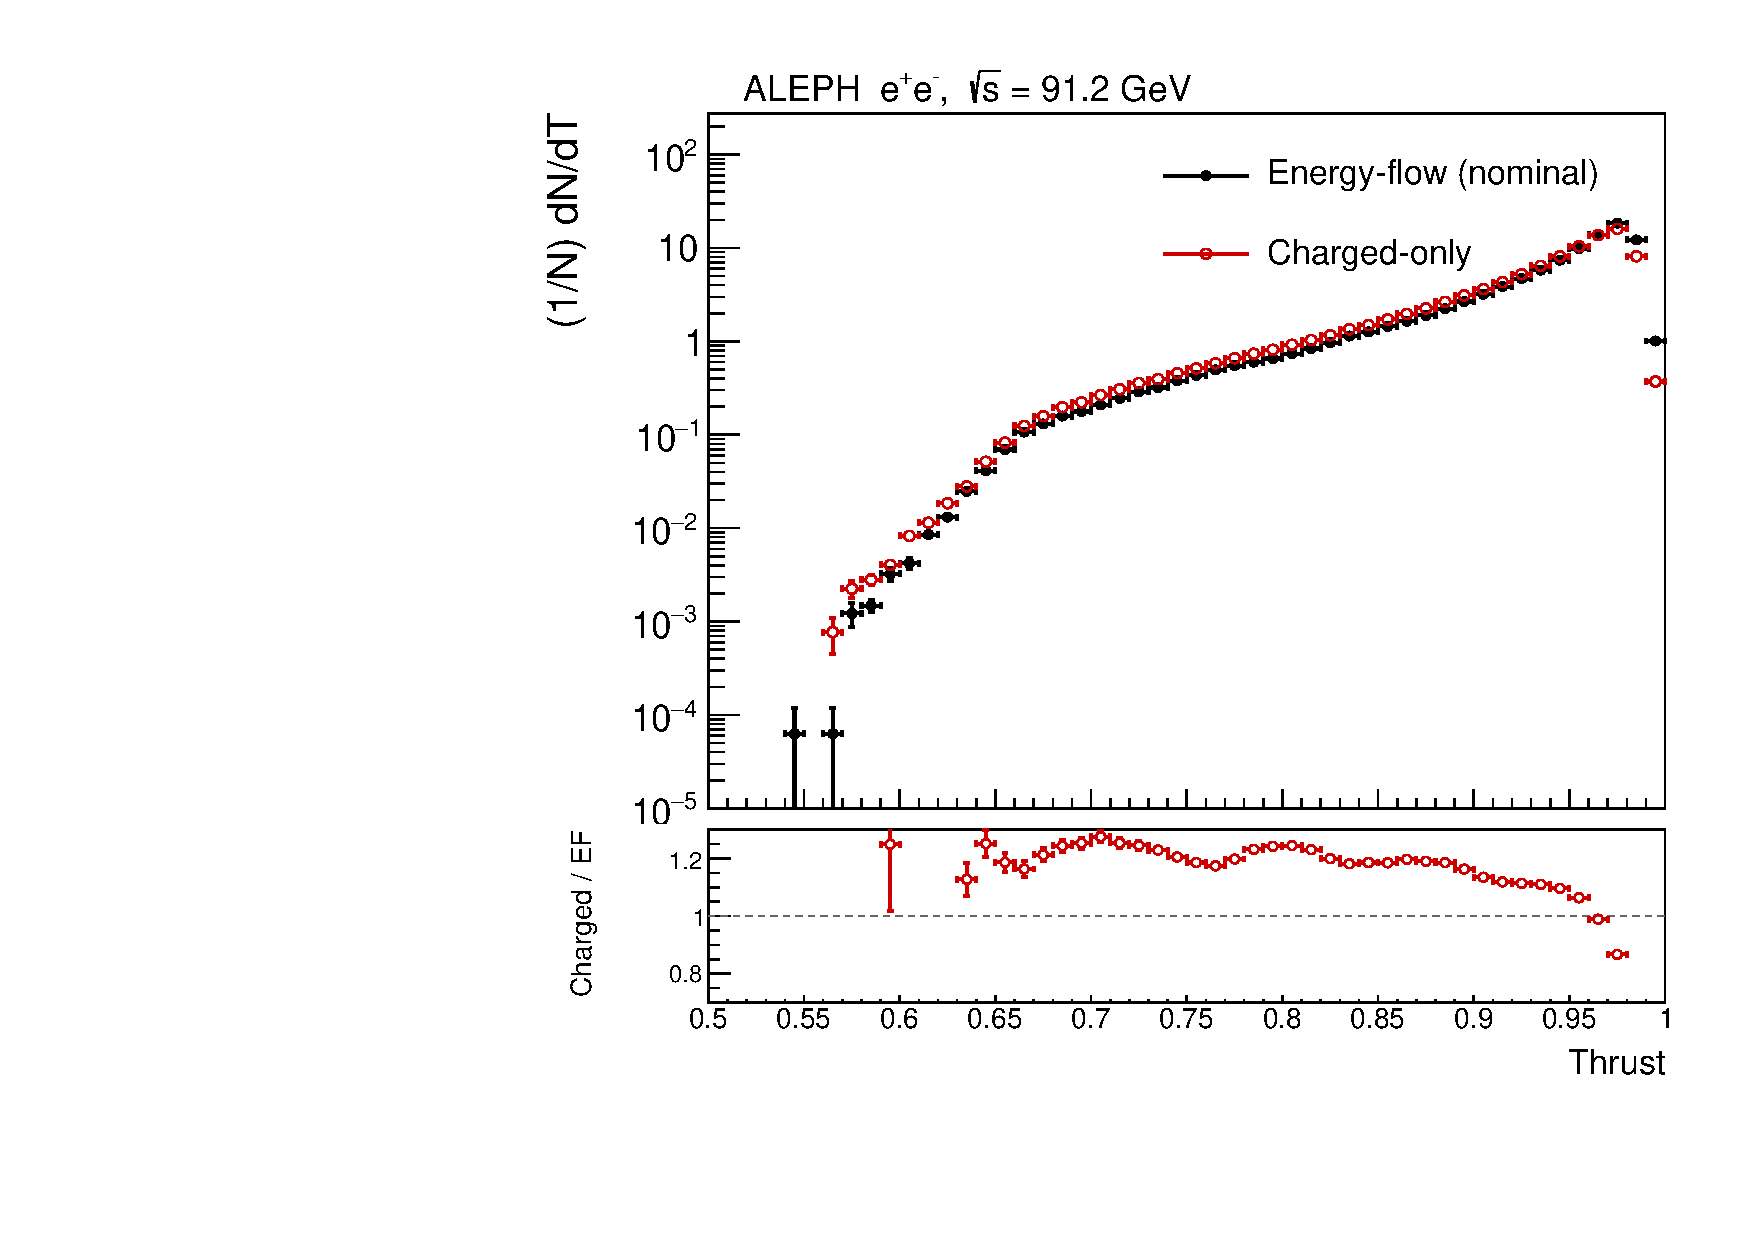
\includegraphics[width=0.70\textwidth]{../Studies/Phase2_Checks_2026-03-03/plots/charged_only_vs_energy_flow/charged_only_vs_energy_flow.pdf}
\caption{Comparison of the charged-only (red open circles) and energy-flow (black filled circles) unfolded thrust distributions, normalized to $(1/N)\,\mathrm{d}N/\mathrm{d}T$.  The ratio panel shows charged-only / energy-flow; the dashed line marks unity.}
\label{fig:charged_vs_ef}
\end{figure}

\FloatBarrier

\subsection{Release products}

The result bundle includes central values, covariance and correlation matrices, binning
definitions, fit-window products, and component-level uncertainty plots. For theory
fits, the recommended inputs are the fit-window covariance products (covering 45 bins
in $0.505\le T < 1.00$) rather than the full-range covariance. All result files are
version-controlled and associated with structured provenance metadata that records the
git commit, software versions, and key analysis parameters used to produce this result.

\section{Conclusion}
\label{sec:conclusion}

A complete thrust-only baseline measurement has been produced with Iterative Bayesian Unfolding on archived ALEPH 1994 data, using nominal $N_{\mathrm{iter}}=5$ and explicit propagation of unfolding, experimental, and theory systematics.

The current result package provides:
\begin{itemize}
\item unfolded central values with hadronic event correction,
\item covariance and correlation matrices for theory-facing use,
\item component-level uncertainty views with individual variation branches,
\item a direct comparison to the published ALEPH thrust result.
\end{itemize}

This establishes a first end-to-end repository baseline for thrust with Iterative Bayesian Unfolding.
It also defines the starting point for extension to C-parameter and heavy-jet mass, including future multidimensional correlation studies.

\section{Challenges with AI-agent analysis}
\label{sec:challenges}

This section is maintained as a living record of unresolved or recurring issues encountered during the analysis and during analyst--agent collaboration. Because this document is an internal note rather than a final publication, we prioritize explicit tracking of weaknesses, mitigation status, and collaboration failure modes.

\subsection{Practical Codex--physicist workflow}

The working model used in this note is a constrained human-in-the-loop cycle:
\begin{enumerate}
\item the physicist defines the physics objective, nominal policy, and acceptance criteria (e.g. nominal IBU iterations, uncertainty definition, figure intent);
\item the agent implements code and note changes, executes reproducible commands, and reports exact file-path and artifact updates;
\item the physicist reviews outputs (plots, numerical consistency, physics interpretation), requests targeted corrections, and approves or rejects the iteration;
\item accepted changes are propagated to the note with explicit script provenance and residual-risk statements.
\end{enumerate}

In this model, authority is intentionally asymmetric: the physicist owns physics choices and release signoff, while the agent owns implementation throughput, consistency checks, and traceability.

\subsection{How interaction is carried out in practice}

The interaction pattern in this project is not free-form chat; it is a specification--execution loop with explicit control points:
\begin{itemize}
\item requests are usually concrete and executable (script, figure, table, section);
\item each iteration requires path-level traceability to scripts, outputs, and note sections;
\item plotting/layout feedback is treated as analysis-relevant, since figure readability affects interpretation;
\item corrections are applied incrementally and revalidated, rather than batching large unreviewed changes;
\item unresolved issues are converted into tracked follow-up tasks rather than hidden in narrative text.
\end{itemize}

This interaction discipline reduced turnaround for code and note updates, but it also exposed repeated bottlenecks in formatting consistency, evolving scope, and ambiguity in implicit expert expectations.

\subsection{Agent-perspective challenges with expert collaboration}

From the agent side, the main recurring challenges are:
\begin{itemize}
\item \textbf{Implicit physics priors}: expert expectations on acceptable binning, regularization behavior, or uncertainty presentation are often assumed rather than initially stated;
\item \textbf{Precision formatting constraints}: small figure-layout details (label offsets, legend placement, pad geometry) require many short feedback loops;
\item \textbf{Method-vs-presentation coupling}: apparent cosmetic changes can alter interpretability and therefore physics conclusions;
\item \textbf{State synchronization risk}: when scripts, outputs, and note text evolve quickly, stale references can appear unless provenance is continuously refreshed;
\item \textbf{Boundary management}: the agent can execute and refactor reliably, but interpretation authority and final scientific claims must remain analyst-owned.
\end{itemize}

These challenge classes are expected in future observable expansions and motivate stricter templating for figures, stronger configuration contracts, and checklists for note updates.

\subsection{Current limitations of the thrust-only baseline}

The present release is robust enough for a preliminary thrust result, but several limitations remain:
\begin{itemize}
\item for events with exactly 3 selected particles, the thrust algorithm selects the highest-magnitude particle as the axis rather than enumerating all possible hemisphere assignments; this approximation is justified because (i) 3-particle hadronic events are rare in $Z \to q\bar{q}$ decays (impact on thrust value typically $\lesssim 0.1\%$ for $T > 0.5$), and (ii) the response-matrix migration structure dominates uncertainty in the endpoint bins where such events concentrate;
\item hadronic-event correction uncertainty is propagated as an independent component ($\Delta_{\mathrm{had}}$, central-range mean $\approx 3.2\%$); the endpoint bins remain sensitive to correction-factor extrapolation;
\item systematic inter-bin correlations use the statistical correlation matrix as a template ($\mathrm{Cov}^{(c)}_{ij} = \Delta_c(i)\,\Delta_c(j)\,\rho^{\mathrm{stat}}_{ij}$); this is an approximation that assumes systematic and statistical correlations share the same bin-to-bin structure;
\item endpoint thrust bins remain statistically and modeling sensitive;
\item analysis scope is currently one-dimensional (thrust only), while the future target includes the thrust-family observables and potentially multidimensional unfolding.
\end{itemize}

\subsection{Persistent analysis challenges}

Several recurrent issues have been tracked through the development of this note. Plot-style consistency across scripts has been an ongoing concern, with centralized style enforcement in producer scripts now largely resolving the issue. Method-to-code traceability gaps are addressed by the workflow and provenance tables in Sec.~\ref{sec:method} and Sec.~\ref{sec:results}, with \path{workflow_summary.json} serving as the canonical numeric record. The most significant open challenge is endpoint-bin instability: the final bin ($0.99<T<1.00$) is sensitive to MC modeling, hadronic correction extrapolation, and normalization convention differences, and dominates the maximum per-bin uncertainty. This is mitigated by reporting central-window metrics ($0.60\le T<0.95$) alongside full-range figures throughout the note.

\subsection{Update protocol for this section}

For each major workflow iteration, this section should record:
\begin{itemize}
\item newly discovered persistent issues;
\item whether previous issues moved from Open to In progress/Resolved;
\item concrete next action and code location for unresolved items.
\end{itemize}

Keeping this log in the main body is intentional: it makes assumptions and remaining risks visible to internal readers and future maintainers.


\bibliographystyle{JHEP}
\bibliography{biblio}

\appendix
\section{Validation and cross-check details}
\label{sec:app_validation}

This appendix collects supplementary validation material that supports the analysis decisions described in the main text.

\subsection{Iteration-scan closure and stability}

The iteration-scan diagnostics used to select $N_{\mathrm{iter}}=5$ are shown in the main text in Figs.~\ref{fig:refold_selected_iters} and~\ref{fig:iteration_choice_diagnostics}. The refolded spectra confirm that $N_{\mathrm{iter}}=5$ reproduces the detector-level data shape within the expected level of statistical fluctuation. The closure-shape $\chi^2/\mathrm{ndf}$ is stable across $N_\mathrm{iter}\in\{4,5,6\}$, and the iteration-to-iteration shift in the unfolded spectrum decreases monotonically before flattening near $N_\mathrm{iter}=5$--$6$, consistent with convergence. The $N_\mathrm{iter}=100$ refolding confirms that the response model does not diverge at high iteration, though the unfolded spectrum in that limit becomes increasingly sensitive to statistical fluctuations.

\subsection{OmniFold and prior IBU comparison}

The comparison with OmniFold and prior Iterative Bayesian Unfolding spectra from \texttt{unfold-ee-logtau/Results} is documented in Sec.~\ref{sec:results} (Fig.~\ref{fig:final_thrust_of_ibu_comparison}). Compatibility metrics are $\chi^2/\mathrm{ndf}=0.663$ (OmniFold), $0.421$ (prior IBU), evaluated over the 42 ALEPH bins using the current total uncertainty model on the diagonal. Differences are localized to the high-thrust endpoint and are consistent with the expected sensitivity of IBU to regularization strength and normalization convention in that region.

\subsection{Difference-check program}

A structured diagnostic program for inter-analysis differences (binning/normalization alignment, hadronic-correction treatment, event/sample synchronization, regularization dependence, and theory-envelope masking) is documented in \path{Plans/2026-02-19_thrust_difference_checks.md}. Execution and acceptance criteria are defined there; no final physics interpretation of residual inter-analysis differences is assigned until that program is completed.

\subsection{Output integrity verification}

After each full workflow run, a dedicated script \texttt{check\_prelim\_summary\_outputs.py} verifies that all required output files are present and non-empty, that the covariance matrix is positive semi-definite on the diagonal, and that the fit mask selects a non-zero number of bins. The 2026-02-17 run passed all checks (1/1 integrity check passed, as recorded in Table~\ref{tab:ai_agent_scorecard}).

\section{Communication summary (reconstructed project-cycle transcript)}
\label{sec:app_communication_summary}

This appendix records a reconstructed full communication summary for the current thrust-analysis cycle.
The source material is the project artifact trail (plans, note rewrites, workflow outputs, and validation products), not a verbatim message log.
The objective is to preserve the decision chain for internal reproducibility and method auditing.

\subsection{Scope and reconstruction sources}

Scope covered: the thrust Iterative Bayesian Unfolding cycle from code review through preliminary-result packaging and note rewrites (Sections 1--8), including the AI-agent collaboration framing.

Primary reconstruction sources:
\begin{itemize}
\item dated planning artifacts under \texttt{Plans/} (2026-02-13 to 2026-02-18);
\item executable workflow outputs in \texttt{Studies/PreliminaryResult/}, with run directory \texttt{2026-03-05\_thrust\_iter5/};
\item note section revision trail in \texttt{AnalysisNote/sections/*.tex};
\item workflow scripts in \texttt{Unfolding/scripts/} and \texttt{Studies/*/scripts/}.
\end{itemize}

\subsection{Reconstructed communication timeline}

\begin{enumerate}
\item \textbf{Initial objective setting (2026-02-13).} The collaboration established a thrust-first execution strategy with Iterative Bayesian Unfolding, complete code review, and a JHEP-style internal-note structure.
\item \textbf{Code-audit phase.} Critical and high-impact defects were identified and fixed (tree defaults, closure mode requirements, return-code handling, systematics path robustness), with findings tracked in \texttt{Plans/2026-02-13\_code\_review\_findings.md}.
\item \textbf{1994 workflow focus.} Execution direction was corrected to run the full 1994 derivation and unfolding chain rather than legacy partial-year paths.
\item \textbf{Nominal-regularization policy convergence.} The cycle converged on nominal $N_{\mathrm{iter}}=5$ with 4/6 as regularization systematic envelope for this thrust preliminary pass.
\item \textbf{Systematics completion requirement.} The scope was expanded to include full experimental and theory branches in the same run-owned output package, with hadronic correction retained in nominal processing.
\item \textbf{Result-style iteration loop.} Multiple rounds of visual QA enforced consistent pad geometry, ratio-panel readability, uncertainty normalization conventions, and legend/text placement for publication-grade interpretation.
\item \textbf{ALEPH comparison integration.} Final-result plotting was upgraded to include ratio to ALEPH 2004 in matched binning with uncertainty propagation via ROOT histogram operations.
\item \textbf{Uncertainty decomposition policy.} The workflow migrated from envelope-only views to explicit component-level plots, including signed shifts, grouped uncertainty structure, and central-window interpretation.
\item \textbf{Section-by-section rewrite cycle (Sections 1--5 first).} The note was expanded with stronger physics motivation, detector/data context, and reconstruction validation text connected directly to thrust sensitivity.
\item \textbf{Sections 5+ hardening.} Methods, systematics, and results sections were restructured for executable traceability (script entrypoints, output paths, and release artifacts).
\item \textbf{AI-agent narrative formalization.} A dedicated section captured operating model, controls, and measurable scorecard, followed by a final chapter logging persistent collaboration and analysis challenges.
\item \textbf{Physics-tone refinement.}\\
Introductory framing was strengthened around precision-QCD motivation,\\
LEP data quality, and validation goals.
\item \textbf{External-citation expansion.}\\
AI-for-science and agent-workflow references were expanded, then extended with requested recent case studies.
\item \textbf{Reproducibility emphasis.} The communication repeatedly enforced path-level provenance for figures and summary products, with explicit checks and output validation scripts.
\item \textbf{Current-cycle layout request.} Results narrative was requested to present uncertainty decomposition before the final unfolded comparison, and to add a final-result total correlation matrix view.
\item \textbf{Current-cycle documentation request.} A complete communication appendix was requested for community context, with highlighted key decisions and rationale.
\end{enumerate}

\subsection{Key exchanges and decisions}

\newcommand{\decisionbox}[3]{%
\noindent\fbox{%
\parbox{0.97\textwidth}{%
\textbf{Decision:} #1\\
\textbf{Rationale:} #2\\
\textbf{Impact:} #3
}}%
}

\decisionbox
{Use Iterative Bayesian Unfolding as the baseline correction method for this cycle.}
{Fast iteration without model retraining was required for rapid experimental cross-check loops.}
{Workflow scripts, method text, and uncertainty propagation were all aligned to IBU.}

\decisionbox
{Set nominal regularization to $N_{\mathrm{iter}}=5$ with 4/6 as regularization systematic.}
{Iteration-scan diagnostics and practical stability/throughput tradeoffs favored this operating point.}
{All nominal and systematic branches, note text, and final plots were normalized to the same policy.}

\decisionbox
{Run the full 1994 chain as the maintained baseline dataset year.}
{The analysis state required consistency in data/MC derivation and response inputs for one complete production year.}
{Output provenance and note references were consolidated under run-owned 1994 directories.}

\decisionbox
{Adopt a strict figure-style contract for result plots (connected pads, controlled ratio range, readable labels).}
{Visual interpretation quality was treated as analysis-relevant, not cosmetic.}
{Several plotting scripts were iteratively corrected until style and uncertainty semantics stabilized.}

\decisionbox
{Promote component-level uncertainty views (statistical, unfolding, experimental, theory) over envelope-only summaries.}
{Readers need source-resolved behavior rather than only combined envelopes.}
{Results section now reports component behavior explicitly and ties interpretation to central-window metrics.}

\decisionbox
{Keep ``no-neutrals'' as a cross-check branch and separate it from nominal total uncertainty.}
{It is a stress test rather than a baseline uncertainty source.}
{Cross-check visibility is preserved while nominal total remains policy-consistent.}

\decisionbox
{Introduce explicit AI-agent operating-model and challenge-tracking sections.}
{The internal-note objective includes evaluating whether an agent can execute research workflows under supervision.}
{The note now contains controls, measurable scorecard, and persistent challenge logging.}

\decisionbox
{Expand citations to include recent AI+scientist and theory-assistant case studies.}
{Program motivation required concrete external evidence beyond generic AI discussion.}
{Introduction and AI-agent sections now cite both broad and recent workflow-relevant studies.}

\decisionbox
{Reorder results narrative to show uncertainty structure before final unfolded comparison.}
{Interpretation of the final spectrum is clearer once uncertainty sources are established first.}
{Section flow now progresses from component structure to correlated final products to central comparison.}

\decisionbox
{Add a final-result total correlation matrix plot from \texttt{corr\_total.csv}.}
{Community-facing usage requires direct visibility of correlated uncertainties after full nominal combination.}
{Release package now includes a dedicated final total-correlation figure and script-level provenance.}

\subsection{Communication-pattern summary}

The reconstructed cycle indicates a high-frequency specification--execution loop with strong emphasis on:
\begin{itemize}
\item explicit physics-policy locking before broader text expansion;
\item figure-level interpretability as a first-class requirement;
\item command/path-level provenance for every released artifact;
\item incremental correction and revalidation rather than large unreviewed batches.
\end{itemize}

The dominant friction points were precision formatting constraints, rapid scope evolution, and synchronization between code outputs and note narrative. These patterns are consistent with the persistent-challenge tracker in Sec.~\ref{sec:challenges}.


\end{document}
